\PassOptionsToPackage{unicode=true}{hyperref} % options for packages loaded elsewhere
\PassOptionsToPackage{hyphens}{url}
\PassOptionsToPackage{dvipsnames,svgnames*,x11names*}{xcolor}
%
\documentclass[]{krantz}
\usepackage{lmodern}
\usepackage{amssymb,amsmath}
\usepackage{ifxetex,ifluatex}
\usepackage{fixltx2e} % provides \textsubscript
\ifnum 0\ifxetex 1\fi\ifluatex 1\fi=0 % if pdftex
  \usepackage[T1]{fontenc}
  \usepackage[utf8]{inputenc}
  \usepackage{textcomp} % provides euro and other symbols
\else % if luatex or xelatex
  \usepackage{unicode-math}
  \defaultfontfeatures{Ligatures=TeX,Scale=MatchLowercase}
\fi
% use upquote if available, for straight quotes in verbatim environments
\IfFileExists{upquote.sty}{\usepackage{upquote}}{}
% use microtype if available
\IfFileExists{microtype.sty}{%
\usepackage[]{microtype}
\UseMicrotypeSet[protrusion]{basicmath} % disable protrusion for tt fonts
}{}
\IfFileExists{parskip.sty}{%
\usepackage{parskip}
}{% else
\setlength{\parindent}{0pt}
\setlength{\parskip}{6pt plus 2pt minus 1pt}
}
\usepackage{xcolor}
\usepackage{hyperref}
\hypersetup{
            pdftitle={Practical Computing and Bioinformatics for Conservation and Evolutionary Genomics},
            pdfauthor={Eric C. Anderson},
            colorlinks=true,
            linkcolor=Maroon,
            filecolor=Maroon,
            citecolor=Blue,
            urlcolor=Blue,
            breaklinks=true}
\urlstyle{same}  % don't use monospace font for urls
\usepackage{color}
\usepackage{fancyvrb}
\newcommand{\VerbBar}{|}
\newcommand{\VERB}{\Verb[commandchars=\\\{\}]}
\DefineVerbatimEnvironment{Highlighting}{Verbatim}{commandchars=\\\{\}}
% Add ',fontsize=\small' for more characters per line
\usepackage{framed}
\definecolor{shadecolor}{RGB}{248,248,248}
\newenvironment{Shaded}{\begin{snugshade}}{\end{snugshade}}
\newcommand{\AlertTok}[1]{\textcolor[rgb]{0.33,0.33,0.33}{#1}}
\newcommand{\AnnotationTok}[1]{\textcolor[rgb]{0.37,0.37,0.37}{\textbf{\textit{#1}}}}
\newcommand{\AttributeTok}[1]{\textcolor[rgb]{0.61,0.61,0.61}{#1}}
\newcommand{\BaseNTok}[1]{\textcolor[rgb]{0.06,0.06,0.06}{#1}}
\newcommand{\BuiltInTok}[1]{#1}
\newcommand{\CharTok}[1]{\textcolor[rgb]{0.5,0.5,0.5}{#1}}
\newcommand{\CommentTok}[1]{\textcolor[rgb]{0.37,0.37,0.37}{\textit{#1}}}
\newcommand{\CommentVarTok}[1]{\textcolor[rgb]{0.37,0.37,0.37}{\textbf{\textit{#1}}}}
\newcommand{\ConstantTok}[1]{\textcolor[rgb]{0,0,0}{#1}}
\newcommand{\ControlFlowTok}[1]{\textcolor[rgb]{0.27,0.27,0.27}{\textbf{#1}}}
\newcommand{\DataTypeTok}[1]{\textcolor[rgb]{0.27,0.27,0.27}{#1}}
\newcommand{\DecValTok}[1]{\textcolor[rgb]{0.06,0.06,0.06}{#1}}
\newcommand{\DocumentationTok}[1]{\textcolor[rgb]{0.37,0.37,0.37}{\textbf{\textit{#1}}}}
\newcommand{\ErrorTok}[1]{\textcolor[rgb]{0.14,0.14,0.14}{\textbf{#1}}}
\newcommand{\ExtensionTok}[1]{#1}
\newcommand{\FloatTok}[1]{\textcolor[rgb]{0.06,0.06,0.06}{#1}}
\newcommand{\FunctionTok}[1]{\textcolor[rgb]{0,0,0}{#1}}
\newcommand{\ImportTok}[1]{#1}
\newcommand{\InformationTok}[1]{\textcolor[rgb]{0.37,0.37,0.37}{\textbf{\textit{#1}}}}
\newcommand{\KeywordTok}[1]{\textcolor[rgb]{0.27,0.27,0.27}{\textbf{#1}}}
\newcommand{\NormalTok}[1]{#1}
\newcommand{\OperatorTok}[1]{\textcolor[rgb]{0.43,0.43,0.43}{\textbf{#1}}}
\newcommand{\OtherTok}[1]{\textcolor[rgb]{0.37,0.37,0.37}{#1}}
\newcommand{\PreprocessorTok}[1]{\textcolor[rgb]{0.37,0.37,0.37}{\textit{#1}}}
\newcommand{\RegionMarkerTok}[1]{#1}
\newcommand{\SpecialCharTok}[1]{\textcolor[rgb]{0,0,0}{#1}}
\newcommand{\SpecialStringTok}[1]{\textcolor[rgb]{0.5,0.5,0.5}{#1}}
\newcommand{\StringTok}[1]{\textcolor[rgb]{0.5,0.5,0.5}{#1}}
\newcommand{\VariableTok}[1]{\textcolor[rgb]{0,0,0}{#1}}
\newcommand{\VerbatimStringTok}[1]{\textcolor[rgb]{0.5,0.5,0.5}{#1}}
\newcommand{\WarningTok}[1]{\textcolor[rgb]{0.37,0.37,0.37}{\textbf{\textit{#1}}}}
\usepackage{longtable,booktabs}
% Fix footnotes in tables (requires footnote package)
\IfFileExists{footnote.sty}{\usepackage{footnote}\makesavenoteenv{longtable}}{}
\usepackage{graphicx,grffile}
\makeatletter
\def\maxwidth{\ifdim\Gin@nat@width>\linewidth\linewidth\else\Gin@nat@width\fi}
\def\maxheight{\ifdim\Gin@nat@height>\textheight\textheight\else\Gin@nat@height\fi}
\makeatother
% Scale images if necessary, so that they will not overflow the page
% margins by default, and it is still possible to overwrite the defaults
% using explicit options in \includegraphics[width, height, ...]{}
\setkeys{Gin}{width=\maxwidth,height=\maxheight,keepaspectratio}
\setlength{\emergencystretch}{3em}  % prevent overfull lines
\providecommand{\tightlist}{%
  \setlength{\itemsep}{0pt}\setlength{\parskip}{0pt}}
\setcounter{secnumdepth}{5}
% Redefines (sub)paragraphs to behave more like sections
\ifx\paragraph\undefined\else
\let\oldparagraph\paragraph
\renewcommand{\paragraph}[1]{\oldparagraph{#1}\mbox{}}
\fi
\ifx\subparagraph\undefined\else
\let\oldsubparagraph\subparagraph
\renewcommand{\subparagraph}[1]{\oldsubparagraph{#1}\mbox{}}
\fi

% set default figure placement to htbp
\makeatletter
\def\fps@figure{htbp}
\makeatother

\usepackage{booktabs}
\usepackage{longtable}
\usepackage[bf,singlelinecheck=off]{caption}

\usepackage{framed,color}
\definecolor{shadecolor}{RGB}{248,248,248}

\renewcommand{\textfraction}{0.05}
\renewcommand{\topfraction}{0.8}
\renewcommand{\bottomfraction}{0.8}
\renewcommand{\floatpagefraction}{0.75}

\renewenvironment{quote}{\begin{VF}}{\end{VF}}
\let\oldhref\href
\renewcommand{\href}[2]{#2\footnote{\url{#1}}}

\makeatletter
\newenvironment{kframe}{%
\medskip{}
\setlength{\fboxsep}{.8em}
 \def\at@end@of@kframe{}%
 \ifinner\ifhmode%
  \def\at@end@of@kframe{\end{minipage}}%
  \begin{minipage}{\columnwidth}%
 \fi\fi%
 \def\FrameCommand##1{\hskip\@totalleftmargin \hskip-\fboxsep
 \colorbox{shadecolor}{##1}\hskip-\fboxsep
     % There is no \\@totalrightmargin, so:
     \hskip-\linewidth \hskip-\@totalleftmargin \hskip\columnwidth}%
 \MakeFramed {\advance\hsize-\width
   \@totalleftmargin\z@ \linewidth\hsize
   \@setminipage}}%
 {\par\unskip\endMakeFramed%
 \at@end@of@kframe}
\makeatother

\renewenvironment{Shaded}{\begin{kframe}}{\end{kframe}}

\usepackage{makeidx}
\makeindex

\urlstyle{tt}

\usepackage{amsthm}
\makeatletter
\def\thm@space@setup{%
  \thm@preskip=8pt plus 2pt minus 4pt
  \thm@postskip=\thm@preskip
}
\makeatother


% Here is stuff for Rmd notes and cautions and things that ECA lifted from
% Yihui's bookdown book
\makeatletter
\@ifundefined{Shaded}{
}{\renewenvironment{Shaded}{\begin{kframe}}{\end{kframe}}}
\makeatother
\newenvironment{rmdblock}[1]
  {
  \begin{itemize}
  \renewcommand{\labelitemi}{
    \raisebox{-.7\height}[0pt][0pt]{
      {\setkeys{Gin}{width=3em,keepaspectratio}\includegraphics{images/#1}}
    }
  }
  \setlength{\fboxsep}{1em}
  \begin{kframe}
  \item
  }
  {
  \end{kframe}
  \end{itemize}
  }
\newenvironment{rmdnote}
  {\begin{rmdblock}{note}}
  {\end{rmdblock}}
\newenvironment{rmdcaution}
  {\begin{rmdblock}{caution}}
  {\end{rmdblock}}
\newenvironment{rmdimportant}
  {\begin{rmdblock}{important}}
  {\end{rmdblock}}
\newenvironment{rmdtip}
  {\begin{rmdblock}{tip}}
  {\end{rmdblock}}
\newenvironment{rmdwarning}
  {\begin{rmdblock}{warning}}
  {\end{rmdblock}}



\frontmatter
\usepackage[]{natbib}
\bibliographystyle{apalike}

\title{Practical Computing and Bioinformatics for Conservation and Evolutionary Genomics}
\author{Eric C. Anderson}
\date{2020-03-31}

\let\BeginKnitrBlock\begin \let\EndKnitrBlock\end
\begin{document}
\maketitle

% you may need to leave a few empty pages before the dedication page

%\cleardoublepage\newpage\thispagestyle{empty}\null
%\cleardoublepage\newpage\thispagestyle{empty}\null
%\cleardoublepage\newpage
\thispagestyle{empty}

\begin{center}

%\includegraphics{images/dedication.pdf}
\end{center}

\setlength{\abovedisplayskip}{-5pt}
\setlength{\abovedisplayshortskip}{-5pt}

{
\hypersetup{linkcolor=}
\setcounter{tocdepth}{2}
\tableofcontents
}
\listoftables
\listoffigures
\newcommand{\bitsfa}{{\circ}{\circ}{\circ}{\bullet}}
\newcommand{\bitsfb}{{\circ}{\circ}{\bullet}{\circ}}
\newcommand{\bitsfc}{{\circ}{\bullet}{\circ}{\circ}}
\newcommand{\bitsfd}{{\bullet}{\circ}{\circ}{\circ}}
\newcommand{\bitsopen}{{\circ}{\circ}{\circ}{\circ}}

\newcommand{\bitsa}{\bitsopen~\bitsopen~\bitsfa}
\newcommand{\bitsb}{\bitsopen~\bitsopen~\bitsfb}
\newcommand{\bitsc}{\bitsopen~\bitsopen~\bitsfc}
\newcommand{\bitsd}{\bitsopen~\bitsopen~\bitsfd}

\newcommand{\bitse}{\bitsopen~\bitsfa~\bitsopen}
\newcommand{\bitsf}{\bitsopen~\bitsfb~\bitsopen}
\newcommand{\bitsg}{\bitsopen~\bitsfc~\bitsopen}
\newcommand{\bitsh}{\bitsopen~\bitsfd~\bitsopen}

\newcommand{\bitsi}{\bitsfa~\bitsopen~\bitsopen}
\newcommand{\bitsj}{\bitsfb~\bitsopen~\bitsopen}
\newcommand{\bitsk}{\bitsfc~\bitsopen~\bitsopen}
\newcommand{\bitsl}{\bitsfd~\bitsopen~\bitsopen}
\newcommand{\bitsmany}{\bitsopen~{\circ}{\bullet}{\circ}{\bullet}~{\circ}{\circ}{\bullet}{\bullet}}

\hypertarget{preface}{%
\chapter*{Preface}\label{preface}}


This is a collection of blurbs Eric started writing in the last year to
help remind himself and others of some useful things to know for bioinformatics.

It was started during an extended government shutdown, when it seemed like writing a book
might be in order. Fortunately, the shutdown ended eventually. It is not clear whether a
book will ever come of it, but these notes shall be up on the web indefinitely, so feel free to use
them!

\hypertarget{intro}{%
\chapter{Introduction}\label{intro}}

Nothing here yet.

\hypertarget{erics-notes-of-what-he-might-do}{%
\chapter{Eric's Notes of what he might do}\label{erics-notes-of-what-he-might-do}}

This is where I am going to just throw out ideas and start to organize them. My thought
was that while I am actually doing bioinformatics, etc. in my normal day-to-day work
I will analyze what I am doing and figure out all the different tools that I am using
and organize that or pedagogy.

\begin{itemize}
\tightlist
\item
  Note: I am going to make a companion repository called \texttt{mega-bioinf-pop-gen-examples}
  that will house all of the data sets and things for exercises.
\end{itemize}

\hypertarget{table-of-topics}{%
\section{Table of topics}\label{table-of-topics}}

Man! There is going to be a lot to get through. My current idea
is to meet three times a week. The basic gist of those three sessions
will be like this:

\begin{enumerate}
\def\labelenumi{\arabic{enumi}.}
\item
  \textbf{Fundamental Tools / Environments}: I am thinking 5 weeks on Unix, 1 Week on HPC, 6 Weeks on R/Rstudio, and 3 on Python from within Rstudio (so that students know enough to run python modules like moments.)
\item
  \textbf{Theory and Background}: Population-genetic and bioinformatic theory. Alignment and BW transforms, the coalescent, Fst, etc. Basically things that are needed to understand (to some degree) what various programs/analyses are doing under the hood.
\item
  \textbf{Application and Practice}: Getting the students to get their feet wet and their fingers dirty actually doing it. This time should be entirely practical, with students doing an exercise (in pairs or groups, possibly) with me (or someone else, maybe CH) overseeing.
\end{enumerate}

\begin{longtable}[]{@{}llll@{}}
\toprule
\begin{minipage}[b]{0.10\columnwidth}\raggedright
Week\strut
\end{minipage} & \begin{minipage}[b]{0.21\columnwidth}\raggedright
Fundamental Tools\strut
\end{minipage} & \begin{minipage}[b]{0.29\columnwidth}\raggedright
Theory and Background\strut
\end{minipage} & \begin{minipage}[b]{0.29\columnwidth}\raggedright
Application and Practice\strut
\end{minipage}\tabularnewline
\midrule
\endhead
\begin{minipage}[t]{0.10\columnwidth}\raggedright
1\strut
\end{minipage} & \begin{minipage}[t]{0.21\columnwidth}\raggedright
\emph{Unix Intro}: filesystem; absolute and relative paths, everything is a file; readable, writable, executable; PATH; .bashrc --- hack everyone's to get the time and directory; TAB-completion; \texttt{cd}, \texttt{ls} (colored output), \texttt{cat}, \texttt{head}, \texttt{less}; stdout and stderr and file redirection of either with \texttt{\textgreater{}} and \texttt{2\textgreater{}}; the \texttt{;} vs \texttt{\&}. Using TextWrangler with \texttt{edit} and we need a PC equivalent\ldots{}\strut
\end{minipage} & \begin{minipage}[t]{0.29\columnwidth}\raggedright
\emph{Data Formats}: fasta, fastq, SAM, BAM, VCF, BCF\strut
\end{minipage} & \begin{minipage}[t]{0.29\columnwidth}\raggedright
Command line drills\strut
\end{minipage}\tabularnewline
\begin{minipage}[t]{0.10\columnwidth}\raggedright
2\strut
\end{minipage} & \begin{minipage}[t]{0.21\columnwidth}\raggedright
Programs, binaries, compiling, installing, package management; software distribution; GitHub and sourceforge; admin privileges and sudo, and how you probably won't have that on a cluster.\strut
\end{minipage} & \begin{minipage}[t]{0.29\columnwidth}\raggedright
Fundamental programming concepts; Scripts vs binaries (i.e.~compiled vs interpreted languages); dependencies: headers and libraries; Modularization; Essential algorithms; compression;\strut
\end{minipage} & \begin{minipage}[t]{0.29\columnwidth}\raggedright
samtools, vcftools, bcftools. hands on, doing stuff with them, reading the man pages, exercises.\strut
\end{minipage}\tabularnewline
\begin{minipage}[t]{0.10\columnwidth}\raggedright
3\strut
\end{minipage} & \begin{minipage}[t]{0.21\columnwidth}\raggedright
\emph{Programming on the shell}: variables and variable substitution; Globbing and path expansion; variable modifications; loops; conditionals;\strut
\end{minipage} & \begin{minipage}[t]{0.29\columnwidth}\raggedright
\strut
\end{minipage} & \begin{minipage}[t]{0.29\columnwidth}\raggedright
\strut
\end{minipage}\tabularnewline
\begin{minipage}[t]{0.10\columnwidth}\raggedright
4\strut
\end{minipage} & \begin{minipage}[t]{0.21\columnwidth}\raggedright
\emph{sed, awk, and regular expressions}\strut
\end{minipage} & \begin{minipage}[t]{0.29\columnwidth}\raggedright
\strut
\end{minipage} & \begin{minipage}[t]{0.29\columnwidth}\raggedright
\strut
\end{minipage}\tabularnewline
\begin{minipage}[t]{0.10\columnwidth}\raggedright
5\strut
\end{minipage} & \begin{minipage}[t]{0.21\columnwidth}\raggedright
\emph{HPC}: clusters; nodes; cores; threads. SGE and/or SLURM; \texttt{qsub}; \texttt{qdel}; \texttt{qacct}; \texttt{myjobs}; job arrays.\strut
\end{minipage} & \begin{minipage}[t]{0.29\columnwidth}\raggedright
\strut
\end{minipage} & \begin{minipage}[t]{0.29\columnwidth}\raggedright
\strut
\end{minipage}\tabularnewline
\bottomrule
\end{longtable}

\mainmatter

\hypertarget{part-part-i-essential-computing-skills}{%
\part{Part I: Essential Computing Skills}\label{part-part-i-essential-computing-skills}}

\hypertarget{overview-of-essential-computing-skills}{%
\chapter{Overview of Essential Computing Skills}\label{overview-of-essential-computing-skills}}

What up with this? It appears that bookdown does not let you
write things at the beginning of a Part without putting it under
a chapter heading. Oh well.

\hypertarget{essential-unixlinux-terminal-knowledge}{%
\chapter{Essential Unix/Linux Terminal Knowledge}\label{essential-unixlinux-terminal-knowledge}}

Unix was developed at AT\&T Bell Labs in the 1960s. Formally ``UNIX'' is a
trademarked operating system,
but when most people talk about ``Unix''
they are talking about the \emph{shell}, which is the text-command-driven interface
by which Unix users interact with the computer.

The Unix shell has been around, largely unchanged, for many decades because it is \emph{awesome}.
When you learn it, you aren't learning a fad, but, rather, a mode of interacting
with your computer that has been time tested and will likely
continue to be the lingua franca of large computer systems
for many decades to come.

For bioinformatics, Unix is the tool of choice for a number of reasons: 1) complex analyses
of data can be undertaken with a minimum of words; 2) Unix allows automation of tasks,
especially ones that are repeated many times; 3) the standard set of Unix commands includes
a number of tools for managing large files and for inspecting and manipulating text files; 4) multiple,
successive analyses upon a single stream of data can be expressed and executed efficiently,
typically without the need to write intermediate results to the disk;
5) Unix was developed when computers were extremely limited in terms of memory and speed. Accordingly,
many Unix tools have been well optimized and are appropriate to the massive genomic data sets
that can be taxing even for today's large, high performance computing systems; 6) virtually all state-of-the-art
bioinformatic tools are tailored to run in a Unix environment; and finally, 7) essentially
every high-performance computer cluster runs some variant of Unix, so if you are going to be
using a cluster for your analyses (which is highly likely), then you have gotta know Unix!

\hypertarget{getting-a-bash-shell-on-your-system}{%
\section{Getting a bash shell on your system}\label{getting-a-bash-shell-on-your-system}}

A special part of the Unix operating system is the ``shell.'' This is the system that
interprets commands from the user. At times it behaves like an interpreted programming
language, and it also has a number of features that help to minimize the amount of
typing the user must do to complete any particular tasks. There are a number of
different ``shells'' that people use. We will focus on one called ``bash,'' which stands
for the ``Bourne again shell.'' Many of the shells share a number of features.

Many common operating systems are built upon a Unix or upon Linux---an open-source flavor of
Unix that is, in many scenarios, indistinguishable. Hereafter we will refer
to both Unix and Linux as ``Unix'' systems). For example all Apple Macintosh computers are
built on top of the Berkeley Standard Distribution of Unix and bash is the default
shell. Many people these days
use laptops that run a flavor of Linux like Ubuntu, Debian, or RedHat. Linux
users should ensure that they are running the bash shell. This can be done
by typing ``bash'' at the command line, or inserting that into their profile.
To know what shell is currently running you can type:

\begin{Shaded}
\begin{Highlighting}[]
\BuiltInTok{echo} \VariableTok{$0}
\end{Highlighting}
\end{Shaded}

at the Unix command line. If you are running \texttt{bash} the result should
be

\begin{Shaded}
\begin{Highlighting}[]
\ExtensionTok{-bash}
\end{Highlighting}
\end{Shaded}

PCs running Microsoft Windows are something of the exception in the computer world, in that
they are not running an operating system built on Unix. However, Windows 10 now allows for
a Linux Subsystem to be run. For Windows, it is also possible to install a lightweight
implementation of bash (like Git Bash). This is helpful for learning how to use Unix,
but it should be noted that most bioinformatic tools are still difficult to install
on Windows.

\hypertarget{navigating-the-unix-filesystem}{%
\section{Navigating the Unix filesystem}\label{navigating-the-unix-filesystem}}

Most computer users will be familiar with the idea of saving documents into ``folders.''
These folders are typically navigated using a ``point-and-click'' interface
like that of the Finder in Mac OS X or the File Explorer in a Windows system.
When working in a Unix shell, such a point-and-click interface is typically not available,
and the first hurdle that new Unix users must surmount is learning to quickly navigate in
the Unix filesystem from a terminal prompt. So,
we begin our foray into Unix and its command prompt with this essential skill.

When you start a Unix shell in a terminal window you get a \emph{command prompt}
that might look something like this:

\begin{Shaded}
\begin{Highlighting}[]
\ExtensionTok{my-laptop}\NormalTok{:~ me$}
\end{Highlighting}
\end{Shaded}

or, perhaps something as simple as:

\begin{Shaded}
\begin{Highlighting}[]
\NormalTok{$}
\end{Highlighting}
\end{Shaded}

or maybe something like:

\begin{Shaded}
\begin{Highlighting}[]
\NormalTok{/}\ExtensionTok{~/--%}
\end{Highlighting}
\end{Shaded}

We will adopt the convention in this book that, unless we are intentionally doing something
fancier, the Unix command prompt is given
by a percent sign, and this will be used when displaying text typed at a command
prompt, followed by output from the command. For example

\begin{Shaded}
\begin{Highlighting}[]
\ExtensionTok{%}\NormalTok{ pwd}
\ExtensionTok{/Users/eriq}
\end{Highlighting}
\end{Shaded}

shows that I issued the Unix command \texttt{pwd}, which instructs the computer to
\textbf{p}rint \textbf{w}orking \textbf{d}irectory, and the computer responded by printing
\texttt{/Users/eriq}, which, on my Mac OS X system is my \emph{home directory}.
In Unix parlance, rather than speaking of ``folders,'' we call
them ``directories;'' however, the two are essentially the same thing.
Every user
on a Unix system has a home directory. It is the domain on a shared computer
in which the user has privileges to create and delete files and do work.
It is where most of your work will happen. When you are working in the Unix
shell there is a notion of a
\emph{current working directory}---that is to say, a place within the hierarchy of
directories where you are ``currently working.'' This will become more concrete
after we have encountered a few more concepts.

The specification \texttt{/Users/eriq} is what is known as an \emph{absolute path}, as it provides the
``address'' of my home directory, \texttt{eriq}, on my laptop, starting from the \emph{root}
of the filesystem. Every Unix computer system has a root directory (you can
think of it as the ``top-most'' directory in a hierarchy), and on every Unix system
this root directory always has the special name, \texttt{/}. The address
of a directory relative to the root is specified by starting with the root (\texttt{/})
and then naming each subsequent directory that you must go inside of in order to
get to the destination, each separated by a \texttt{/}. For example, \texttt{/Users/eriq}
tells us that we start at the root (\texttt{/}) and then we go into the \texttt{Users} directory
(\texttt{Users}) and then, from there, into the \texttt{eriq} directory. Note that \texttt{/} is used to mean the root
directory when at the beginning of an absolute path, but in the remainder of the path
its meaning is different: it is used merely as a separator
between directories nested within one another. Figure~\ref{fig:file-hierarchy} shows
an example hierarchy of some of the directories that are found on the author's
laptop.

\begin{figure}

{\centering 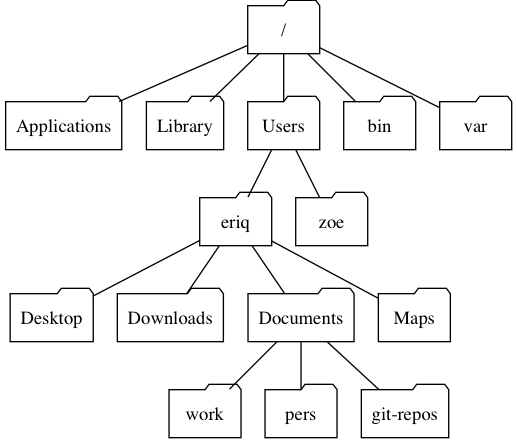
\includegraphics{figs/file-hierarchy} 

}

\caption{A partial view of the directories on the author's laptop.}\label{fig:file-hierarchy}
\end{figure}

From this perspective it is obvious that the directory \texttt{eriq} lives inside \texttt{Users}, and also that, for example,
the absolute path of the directory \texttt{git-repos} would be \texttt{/Users/eriq/Documents/git-repos}.

Absolute paths give the precise location of a directory relative to the root of the filesystem,
but it is not always convenient, nor appropriate, to work entirely with absolute paths.
For one thing, directories that are deeply nested within many others can have long and unwieldy
absolute path names that are hard to type and can be difficult to remember. Furthermore, as we will
see later in this book, absolute paths are typically not \emph{reproducible} from one computer's
filesystem to another. Accordingly, it is more common to give the address of directories using
\emph{relative paths}. Relative paths work much like absolute paths; however, they do not start with
a leading \texttt{/}, and hence they do not take as their
starting point the root directory. Rather, their starting point is implicitly taken
to be the current working directory. Thus, if the current working directory is
\texttt{/Users/eriq}, then the path \texttt{Documents/pers} is a relative path to the
\texttt{pers} directory, as can again be seen in Figure~\ref{fig:file-hierarchy}.

The special relative path symbol \texttt{..} means ``the directory that is one level higher up
in the hierarchy.'' So, if the current working directory were \texttt{/Users/eriq/Documents/git-repos},
then the path \texttt{..} would mean \texttt{/Users/eriq/Documents}, the path
\texttt{../work} gives the directory \texttt{/Users/eriq/Documents/work}, and, by using two or more \texttt{..} symbols
separated by forward slashes, we
can even go up multiple levels in the hierarchy: \texttt{../../../zoe} is a relative path for
\texttt{/Users/zoe}, when the current working directory is \texttt{/Users/eriq/Documents/git-repos}.

When naming paths, another
useful Unix shorthand is \texttt{\textasciitilde{}} (a tilde) which denotes the user's home directory. This is particularly
useful since most of your time in a Unix filesystem will be spent in a directory within your
home directory. Accordingly, \texttt{\textasciitilde{}/Documents/work} is a quick shorthand for
\texttt{/Users/eriq/Documents/work}. This is essential practice if you are working on a large shared computing
resource in which the absolute path to your home directory might be changed by the
system administrator when restructuring the filesystem.

\BeginKnitrBlock{rmdtip}
\textbf{A useful piece of terminology:} in any path, the ``final'' directory
name is called the \emph{basename} of the path. Hence the basename of \texttt{/Users/eriq/Documents/git-repos}
is \texttt{git-repos}. And the basename of \texttt{../../Users} is \texttt{Users}.
\EndKnitrBlock{rmdtip}

\hypertarget{changing-the-working-directory-with-cd}{%
\subsection{\texorpdfstring{Changing the working directory with \texttt{cd}}{Changing the working directory with cd}}\label{changing-the-working-directory-with-cd}}

When you begin a Unix terminal session, the current working
directory is set, by default, to your home directory. However, when you are doing
bioinformatics or otherwise hacking on the command line, you will typically
want to be ``in another directory'' (meaning you will want the current working
directory set to some other directory). For this, Unix provides the \texttt{cd} command, which
stands for \textbf{c}hange \textbf{d}irectory. The syntax is super simple:

cd \emph{path}

where \emph{path} is an absolute or a relative path. For example, to
get to the \texttt{git-repos} directory from my home directory would require
a simple command \texttt{cd\ Documents/git-repos}. Once there, I could change to
my \texttt{Desktop} directory with \texttt{cd\ ../../Desktop}. Witness:

\begin{Shaded}
\begin{Highlighting}[]
\ExtensionTok\NormalTok{ cd Documents/git-repos/}
\ExtensionTok\NormalTok{ cd ../../Desktop}
\ExtensionTok{%}\NormalTok{ pwd}
\ExtensionTok{/Users/eriq/Desktop}
\end{Highlighting}
\end{Shaded}

Once you have used \texttt{cd}, the working directory of your current shell will
remain the same no matter how many other commands you issue,
until you invoke the \texttt{cd} command another time and change
to a different directory.

If you give the \texttt{cd} command with no path specified, your working directory
will be set to your home directory. This is super-handy if you have been
exploring the levels of a Unix filesystem above your home directory and cannot
remember how to get back to your home directory. Just remember that

\begin{Shaded}
\begin{Highlighting}[]
\ExtensionTok{%}\NormalTok{ cd}
\end{Highlighting}
\end{Shaded}

will get you back home.

Another useful shortcut is to supply \texttt{-} (a hyphen) as the path to \texttt{cd}. This will
change the working directory back to where you were before your last invocation
of \texttt{cd}, and it will tell you which directory you have returned to. For example, if you start in \texttt{/Users/eriq/Documents/git-repos} and then
\texttt{cd} to \texttt{/bin}, you can get back to \texttt{git-repos} with \texttt{cd\ -} like so:

\begin{Shaded}
\begin{Highlighting}[]
\ExtensionTok\NormalTok{ cd /bin/}
\ExtensionTok\NormalTok{ cd -}
\ExtensionTok{/Users/eriq/Documents/git-repos}
\ExtensionTok{%}\NormalTok{ pwd}
\ExtensionTok{/Users/eriq/Documents/git-repos}
\end{Highlighting}
\end{Shaded}

Note the output of \texttt{cd\ -} is the newly-returned-to current working directory.

\hypertarget{updating-your-command-prompt}{%
\subsection{Updating your command prompt}\label{updating-your-command-prompt}}

When you are buzzing around in your filesystem, it is often difficult to remember
which directory you are in. You can always type \texttt{pwd} to figure that out,
but the bash shell also provides a way to print the current working directory
\emph{within your command prompt}.

For example, the command:

\begin{Shaded}
\begin{Highlighting}[]
\VariableTok{PS1=}\StringTok{'[\textbackslash{}W]--% '}
\end{Highlighting}
\end{Shaded}

redefines the command prompt to be the basename of the current directory surrounded
by brackets and followed by \texttt{-\/-\%}:

\begin{Shaded}
\begin{Highlighting}[]
\ExtensionTok\NormalTok{ PS1=}\StringTok{'[\textbackslash{}W]--% '}
\NormalTok{[}\ExtensionTok{git-repos}\NormalTok{]--% cd ../}
\NormalTok{[}\ExtensionTok{Documents}\NormalTok{]--% cd ../}
\NormalTok{[}\ExtensionTok{~}\NormalTok{]}\ExtensionTok{--%}\NormalTok{ cd ../}
\NormalTok{[}\ExtensionTok{Users}\NormalTok{]--% }
\end{Highlighting}
\end{Shaded}

This can make it considerably easier to keep track of where you are in your file system.

We will discuss later how to invoke this change automatically in every terminal session
when we talk about customizing environments in Section~\ref{unix-env}.

\hypertarget{tab-completion-for-paths}{%
\subsection{TAB-completion for paths}\label{tab-completion-for-paths}}

Let's be frank\ldots{}typing path names in order to change from one directory to another can feel
awfully tedious, especially when your every neuron is screaming, ``Why can't I just have a friggin' Finder
window to navigate in!'' Do not despair. This is a normal reaction when you first start using Unix.
Fortunately, Unix file-system navigation can be made much less painful (or even enjoyable)
for you by becoming a master of \emph{TAB-completion}. Imagine the Unix shell is watching
your every keystroke and trying to guess what you are about to type. If you type the first part
of a directory name after a command like \texttt{cd} and then hit the TAB key, the shell will respond
with its best guess of how you want to complete what you are typing.

Take the file hierarchy of Figure~\ref{fig:file-hierarchy}, and imagine that we are in the root
directory. At that point, if we type \texttt{cd\ A}, the shell will think "Ooh! I'll bet they want to
change into the directory \texttt{Applications} because that is the only directory that starts with \texttt{A}. Sure enough,
if you hit TAB, the shell adds to the command line so that \texttt{cd\ A} becomes \texttt{cd\ Applications/}
and the cursor is still waiting for further input at the end of the command.
Boom! That was way easier (and more accurate) than typing all those letters after \texttt{A}.

Developing a lightning-fast TAB-completion trigger finger is, quite seriously, essential to surviving and
thriving in Unix. Use your left pinky to hit TAB. Hone your skills. Make sure you can hit TAB with your eyes
closed. TAB early and TAB often!

Once you can hit TAB instantly from within the middle of any phrase, you
will also want to understand a few simple rules of TAB completion:

\begin{enumerate}
\def\labelenumi{\arabic{enumi}.}
\item
  If you try TAB-completing a word on the command line that is not at the beginning
  of the command line (i.e., you are typing a word after a command like \texttt{cd}), then the shell
  tries to complete the word with a \emph{directory name} or a \emph{file name}.
\item
  The shell will only complete an \emph{entire} directory or file name if the name \emph{uniquely} matches the first part of the
  path that has been entered. In our example, there were no other directories than \texttt{Applications} in \texttt{/} that start
  with \texttt{A}, so the shell was certain that we must have been going for \texttt{Applications}.
\item
  If there is more than one directory or file name that matches what you have already typed, then, the first
  time you hit TAB, nothing happens, but the \emph{second} time you hit TAB, the shell will print a list of
  names that match what you have written so far. For example, in our Figure~\ref{fig:file-hierarchy} example,
  hitting TAB after typing \texttt{cd\ \textasciitilde{}/D} does nothing. But the second time we hit TAB we get a list of
  matching names:

\begin{Shaded}
\begin{Highlighting}[]
\ExtensionTok{%}\NormalTok{ cd ~/D}
\ExtensionTok{Desktop/}\NormalTok{  Documents/  Downloads/}
\end{Highlighting}
\end{Shaded}

  So, if we are heading to \texttt{Documents} we can see that adding \texttt{oc} to our command line, to create \texttt{cd\ Doc} would be sufficient to allow the shell to
  uniquely and correctly guess where we are heading. \texttt{cd\ Doc} will TAB-complete into \texttt{cd\ Documents/}
\item
  If there are multiple directory or file names that match the current command line, and they share
  more letters than those currently on the command line, TAB-completion will complete
  the name to the end of the shared portion of the name. An example helps: let's say
  I have the following two directories with hideously long names in my \texttt{Downloads} folder:

\begin{Shaded}
\begin{Highlighting}[]
\ExtensionTok{WIFL.rep_indiv_est.mixture_collection.count.gr8-results}
\ExtensionTok{WIFL.rep_indiv_est.mixture_collection.count-results}
\end{Highlighting}
\end{Shaded}

  Then, TAB completing on \texttt{\textasciitilde{}/Downloads/WIFL.rep} will partially complete so that the prompt and command look like:

\begin{Shaded}
\begin{Highlighting}[]
\ExtensionTok\NormalTok{ cd ~/Downloads/WIFL.rep_indiv_est.mixture_collection.count}
\ExtensionTok{WIFL.rep_indiv_est.mixture_collection.count-results}
\ExtensionTok{WIFL.rep_indiv_est.mixture_collection.count.gr8-results}
\end{Highlighting}
\end{Shaded}

  At this point, adding \texttt{-} and TAB completing will give the first of those directories.
\end{enumerate}

The last example shows just how much typing TAB completion can save you. So, don't be
shy about hitting that TAB key. When navigating your filesystem (or writing longer command
lines that require paths of files) you should consider hitting TAB after every 1 or 2 letters.
In routine work on the command line, probably somewhere around 25\% or more of my keystrokes
are TABs. Furthermore, a TAB is never going to execute a command, and it typically won't
complete to a path that you don't want (unless you got the first part of its name wrong), so there
isn't any risk to hitting TAB all the time.

\hypertarget{listing-the-contents-of-a-directory-with-ls}{%
\subsection{\texorpdfstring{Listing the contents of a directory with \texttt{ls}}{Listing the contents of a directory with ls}}\label{listing-the-contents-of-a-directory-with-ls}}

So far we have been focusing mostly on directories. However, directories themselves
are not particularly interesting---they are merely containers. It is the \emph{files} inside of directories
that we typically work on. The command \texttt{ls} lists the contents---typically files or
other directories---within a directory.

Invoking the \texttt{ls} command without any other arguments (without anything after it)
returns the contents of the current working directory. In our example,
if we are in \texttt{/Users} then we get:

\begin{Shaded}
\begin{Highlighting}[]
\ExtensionTok\NormalTok{ ls}
\ExtensionTok{bam}\NormalTok{                      map-sliced-fastqs-etc.sh}
\ExtensionTok{bam-slices}\NormalTok{               play}
\ExtensionTok{bwa-run-list.txt}\NormalTok{         REDOS-map-sliced-fastqs-etc.sh}
\ExtensionTok{fastq-file-prefixes.txt}\NormalTok{  sliced}
\ExtensionTok{fqslice-22.error}\NormalTok{         slice-fastqs.sh}
\ExtensionTok{fqslice-22.log}\NormalTok{           slicer-lines.txt}
\ExtensionTok{map-etc.sh}\NormalTok{               Slicer-Logs-summary.txt}
\end{Highlighting}
\end{Shaded}

The first line shows the command prompt and the command: \texttt{\%\ ls}, and the remainder is
the output of the command.

Invoked without any further arguments, the \texttt{ls}
command simply lists the contents of the current working directory. However,
you can also direct \texttt{ls} to list the contents of another directory by simply
adding the path (absolute or relative) of that directory on the command line. For example, continuing with
the example in Figure~\ref{fig:file-hierarchy}, when we are in the home directory (\texttt{eriq})
we can see the directories/files
contained within \texttt{Documents} like so:

\begin{Shaded}
\begin{Highlighting}[]
\NormalTok{[}\ExtensionTok{~}\NormalTok{]}\ExtensionTok{--%}\NormalTok{ ls Documents}
\ExtensionTok{git-repos/}\NormalTok{   pers/   work/}
\end{Highlighting}
\end{Shaded}

If you give paths to more than one directory as arguments to \texttt{ls}, then
the contents of each directory are listed after a heading line that gives
the directory's path (as given as an argument to \texttt{ls}), followed by a colon. For example:

\begin{Shaded}
\begin{Highlighting}[]
\NormalTok{[}\ExtensionTok{~}\NormalTok{]}\ExtensionTok{--%}\NormalTok{ ls Documents/git-repos Documents/work}
\ExtensionTok{Documents}\NormalTok{/git-repos:}
\ExtensionTok{ARCHIVED_mega-bioinf-pop-gen.zip}\NormalTok{  lowergranite_0.0.1.tar.gz}
\ExtensionTok{AssignmentAdustment/}\NormalTok{              mega-bioinf-pop-gen-examples/}
\ExtensionTok{CKMRsim/}\NormalTok{                          microhaps_np/}

\ExtensionTok{Documents}\NormalTok{/work:}
\ExtensionTok{assist/}\NormalTok{          maps/            oxford/          uw_days/}
\ExtensionTok{courses_audited/}\NormalTok{ misc/            personnel/}
\end{Highlighting}
\end{Shaded}

You might also note in the above example, that some of the paths listed within
each of the two directories are followed by a slash, \texttt{/}. This \texttt{ls} customization denotes that
they are directories themselves. Much like your command prompt, \texttt{ls} can be customized in ways
that make its output more informative. We will return to that in Section~\ref{unix-env}.

If you pass the path of a file to \texttt{ls}, and that file exists in your filesystem,
then \texttt{ls} will respond by printing the file's path:

\begin{Shaded}
\begin{Highlighting}[]
\ExtensionTok\NormalTok{ ls Documents/try-this-name}
\ExtensionTok{ls}\NormalTok{: Documents/try-this-name: No such file or directory}
\end{Highlighting}
\end{Shaded}

The multi-column, default output of \texttt{ls} is useful when you want
to scan the contents of a directory, and quickly see as many files
as possible in the fewest lines of output.
However, this output format is not well
structured. For example, you don't know how many columns are going to be used in
the default output of \texttt{ls} (that
depends on the length of the filenames and the width of your terminal), and it
offers little information beyond the names of the files.

You can tell the \texttt{ls} command to provide more information, by using it with the \texttt{-l}
option. Appropriately, with the \texttt{-l} option, the \texttt{ls} command will return
output in \emph{long} format:

\begin{Shaded}
\begin{Highlighting}[]
\ExtensionTok{2019-02-08}\NormalTok{ 21:09 /osu-chinook/--% ls -l}
\ExtensionTok{total}\NormalTok{ 108}
\ExtensionTok{drwxr-xr-x}\NormalTok{  2 eriq kruegg  4096 Feb  7 08:26 bam}
\ExtensionTok{drwxr-xr-x}\NormalTok{ 14 eriq kruegg  4096 Feb  8 15:56 bam-slices}
\ExtensionTok{-rw-r--r--}\NormalTok{  1 eriq kruegg 17114 Feb  7 20:16 bwa-run-list.txt}
\ExtensionTok{-rw-r--r--}\NormalTok{  1 eriq kruegg   824 Feb  6 14:14 fastq-file-prefixes.txt}
\ExtensionTok{-rw-r--r--}\NormalTok{  1 eriq kruegg     0 Feb  7 20:14 fqslice-22.error}
\ExtensionTok{-rw-r--r--}\NormalTok{  1 eriq kruegg     0 Feb  7 20:14 fqslice-22.log}
\ExtensionTok{-rwxr--r--}\NormalTok{  1 eriq kruegg  1012 Feb  7 07:59 map-etc.sh}
\ExtensionTok{-rwxr--r--}\NormalTok{  1 eriq kruegg  1138 Feb  7 20:56 map-sliced-fastqs-etc.sh}
\ExtensionTok{drwxr-xr-x}\NormalTok{  3 eriq kruegg  4096 Feb  7 13:01 play}
\ExtensionTok{-rwxr--r--}\NormalTok{  1 eriq kruegg  1157 Feb  8 15:08 REDOS-map-sliced-fastqs-etc.sh}
\ExtensionTok{drwxr-xr-x}\NormalTok{ 14 eriq kruegg  4096 Feb  8 15:49 sliced}
\ExtensionTok{-rwxr--r--}\NormalTok{  1 eriq kruegg   826 Feb  7 20:09 slice-fastqs.sh}
\ExtensionTok{-rw-r--r--}\NormalTok{  1 eriq kruegg  1729 Feb  7 16:11 slicer-lines.txt}
\end{Highlighting}
\end{Shaded}

Each row contains information about only a single file.
The first column indicates what kind of file
each entry is, and also tells us which users have permission to
do certain things with the file (more on this in a few sections).
The third and fourth columns show that the owner of
each file is \texttt{eriq}, who is a user in the group called \texttt{kruegg}. After that
is the size of the file (in bytes) and the date and time it was last modified.

There are a few options to \texttt{ls} that are particularly useful. One is \texttt{-a}, which causes
\texttt{ls} to include in its listing all files, even \emph{hidden} ones. In a Unix file system,
any file whose name starts with a \texttt{.} is considered a \emph{hidden} file. Commonly, such
files are configuration files or other files used by programs that you typically
don't interact with directly. (We will see an example of this when we start working with \texttt{git} for version control, Section~\ref{git-workings}.) The \texttt{-d} option for \texttt{ls} is also'
quite handy. Recall that when you provide the name of a directory as an argument to \texttt{ls},
the default behavior is to list the contents of the directory. This can be troublesome
when you are listing the contents of a subdirectory: \texttt{ls\ \textasciitilde{}/Documents/git-repos/*} lists the
contents (which can be substantial) of each of the directories in my directory, but
I might only want to know the name of each of those directories, rather than their full contents.
\texttt{ls\ -d\ \textasciitilde{}/Documents/git-repos} will do that for you. Finally, the \texttt{-R} option to \texttt{ls} will cause the operating system to drill down, \emph{recursively} into all the subdirectories of the one you
supplied to the command, and list their contents, as well.

\hypertarget{globbing}{%
\subsection{Globbing}\label{globbing}}

If you have ever had to move a large number of files of a certain type from
one folder to another in a Finder window, you know that individually clicking and
selecting each one and then dragging them can be a tedious task (not to mention the disaster
that ensues if you slip on your mouse and end up dropping all the files some place
you did not intend). Unix provides a wonderful system called \emph{filename expansion} or
``globbing'' for quickly providing the names of a large number of files and paths which let's
you operate on multiple files quickly and efficiently. In short, globbing allows for
\emph{wildcard matching} in path names. This means that you can
specify multiple files that have names that share a common part, but differ in other parts.

The most widely used (and the most permissive) wildcard is the asterisk, \texttt{*}. It matches
anything in a file name. So, for example:

\begin{itemize}
\tightlist
\item
  \texttt{*.vcf} will expand to any files in the current directory with the suffix \texttt{.vcf}.
\item
  \texttt{D*s} will expand to any files that start with an uppercase \texttt{D} and end with an \texttt{s}.
\item
  \texttt{*output-*.txt} will expand to any files that include the phrase \texttt{output-} somewhere
  in their name and also end with \texttt{.txt}.
\item
  \texttt{*} will expand to all files in the current working directory.
\item
  \texttt{/usr/local/*/*.sh} will expand to any files ending in \texttt{.sh} that reside within any directory that
  is within the \texttt{/usr/local} directory.
\end{itemize}

\BeginKnitrBlock{rmdnote}
\textbf{Actually, there is some arcana here:} Names of files or directories that start with a
dot (a period) will not expand unless the
dot is included explicitly. Files with names starting with a dot are
``hidden'' files in Unix. You also will not see them in the results of \texttt{ls}, unless you
use the \texttt{-a} option: \texttt{ls\ -a}.
\EndKnitrBlock{rmdnote}

After the asterisk, the next most commonly-used wildcard is the question mark, \texttt{?}. The question mark
denotes any single character in a file name. For example. If you had a series of files that looked
like \texttt{AA-file.txt}, \texttt{AB-file.txt}, \ldots{}, \texttt{AZ-file.txt}. You could get get all those by
using \texttt{A?-file.txt}. This would not expand to, for example, \texttt{AAZ-file.txt}, if that were in the directory.

You can be more specific in globbing by putting things within \texttt{{[}} and \texttt{{]}}. For example:
\texttt{A{[}A-D{]}*} would pick out any files starting with, \texttt{AA}, \texttt{AB}, \texttt{AC}, or \texttt{AD}. Or you could
have said \texttt{A{[}a-d{]}*} which would get any files starting with \texttt{Aa}, \texttt{Ab}, \texttt{Ac}, or \texttt{Ad}. And you
can also do it with numbers: \texttt{{[}0-9{]}}. You can also negate the contents of the \texttt{{[}{]}}, with \texttt{\^{}}. Thus,
\texttt{100\_{[}\^{}ABC{]}*} picks out all files that start with \texttt{100\_} followed by anything that is \emph{not} and \texttt{A}, \texttt{B}, or a \texttt{C}.

Finally, you can be really specific about replacements in file names by iterating over
different possibilities with a comma-separated list within curly braces. For example, \texttt{img.\{png,jpg,svg\}}
will iterate over the values in curly braces and expand to \texttt{img.png\ img.jpg\ img.svg}. Interestingly,
with curly braces, this forms all those file names whether they exist or not. So, unlike \texttt{*} it isn't
really matching available file names.

The last thing to note about all of these globbing constructs is that they are not intimately
associated with the \texttt{ls} command. Rather, they simply provide expansions on the command
line, and the the \texttt{ls} command is listing all those files. For example, try \texttt{echo\ *.txt}.

\hypertarget{what-makes-a-good-file-name}{%
\subsection{What makes a good file-name?}\label{what-makes-a-good-file-name}}

If the foregoing discussion suggests to you that it might not be good to use an
actual \texttt{*}, \texttt{?}, \texttt{{[}}, or \texttt{\{} in names that you give to files and directories
on your Unix system, then congratulations on your intuition! Although you can use
such characters in your filenames, they have to be preceded by a backslash, and it
gets to be a huge hassle. So don't use them in your file names. Additionally,
characters such as \texttt{\#}, \texttt{\textbar{}}, and \texttt{:} do not play well for file names. Don't use them!

Another pet peeve of mine (and anyone who uses Unix) are file names that have spaces in them.
In Windows and on a Mac it is easy to create file names that have spaces in them. In fact, the
standard Windows system comes with such space-containing directory names as \texttt{My\ Documents} or \texttt{My\ Pictures}. Yikes! Please \emph{don't ever do that in your Unix life!} One can deal with spaces in file
names, but there is really no reason to include spaces in your file names, and having spaces in file
names will typically break a good many scripts. Rather than a space, use an underscore, \texttt{\_}, or a
dash, \texttt{-}. You've gotta admit that, not only does \texttt{My-Documents} work better, but it actually
looks better too!

However, should you have to deal with files having spaces in their name, you can
address them by either backslash escaping the spaces, or putting the whole
file name in quotation marks (single or double quotation marks will work).
If you have a file called \texttt{dumb\ file\ name.jpg}, you can address it on the
command line as either of the following three:

\begin{Shaded}
\begin{Highlighting}[]
\ExtensionTok{dumb\textbackslash{} file\textbackslash{} name.jpg}
\StringTok{"dumb file name.jpg"}
\StringTok{'dumb file name.jpg'}
\end{Highlighting}
\end{Shaded}

To make your life easier, however, the bottom line is that you should name your files
on a Unix system using only upper- and lowercase letters (Unix file systems are
case-sensitive), numerals, and the following three punctuation characters: \texttt{.}, \texttt{-}, and \texttt{\_}.
Though you can use other punctuation characters, they often require special treatment, and it
is better to avoid them altogether.

\hypertarget{the-anatomy-of-a-unix-command}{%
\section{The anatomy of a Unix command}\label{the-anatomy-of-a-unix-command}}

Nearly every Unix command that you might invoke follows a certain pattern. First comes
the \texttt{command} itself. This is the word that tells the system the name of the command
that you are actually trying to do. After that, often, you will provide a series
of \emph{options} that will modify the behavior of the command (for example, as we have seen, \texttt{-l}
is an option to the \texttt{ls} command). Finally, you might then provide some \emph{arguments} to the
functions. These are typically paths to files or directories that you would like the
command to operate on. So, in short, a typical Unix command invocation will look
like this:

\texttt{command} \emph{options} \emph{arguments}

Of course, there are exceptions. For example, when invoking Java-based programs from your
shell, arguments might be supplied in ways that make them look like options, etc. But, for
the most part, the above is a useful way of thinking about Unix commands.

Sometimes, especially when using \texttt{samtools} or \texttt{bcftools}, the \texttt{command} part of the
command line might including a command and a subcommand, like \texttt{samtools\ view} or
\texttt{bcftools\ query}. This means that the operating system is calling the program
\texttt{samtools} (for example), and then samtools interprets the next token (\texttt{view}) to
know that it needs to run the \texttt{view} routine, and interpret all following
options in that context.

We will now break down each element in ``\texttt{command} \emph{options} \emph{arguments}''.

\hypertarget{anatomy-command}{%
\subsection{\texorpdfstring{The \texttt{command}}{The command}}\label{anatomy-command}}

When you type a command at the Unix prompt, whether it is a command like \texttt{ls} or
one like \texttt{samtools} (Section \ref{samtools}), the Unix system has to search around
the filesystem for a file that matches the command name and which provides the actual
instructions (the computer code, if you will) for what the command will actually do.
It cannot be stressed enough how important it is to
understand where and how the bash shell searches for these command files. Understanding this
well, and knowing how to add directories that the shell searches for executable
commands will alleviate a lot of frustration that often arises with Unix.

In brief, all Unix shells (and the bash shell specifically) maintain what is called
an \emph{environment variable} called \texttt{PATH} that is a colon-separated list of pathnames
where the shell searches for commands. You can print the \texttt{PATH} variable using
the \texttt{echo} command:

\begin{Shaded}
\begin{Highlighting}[]
\BuiltInTok{echo} \VariableTok{$PATH}
\end{Highlighting}
\end{Shaded}

On a freshly installed system without many customizations the \texttt{PATH} might look like:

\begin{Shaded}
\begin{Highlighting}[]
\ExtensionTok{/usr}\NormalTok{/bin:/bin:}\ExtensionTok{/usr}\NormalTok{/sbin:}\ExtensionTok{/sbin}
\end{Highlighting}
\end{Shaded}

which is telling us that, when bash is searching for a command, it searches for a file
of the same name as the command first in the directory \texttt{/usr/bin}. If it finds it there, then
it uses the contents of that file to invoke the command. If it doesn't find it there,
then it next searches for the file in directory \texttt{/bin}. If it's not there, it searches
in \texttt{/usr/sbin}, and finally in \texttt{/sbin}. If it does not find the command in any of those directories
then it returns the error \texttt{command\ not\ found}.

When you install programs on your own computer system, quite often the installer will modify
a system file that specifies the \texttt{PATH} variable upon startup. Thus after installing some
programs that use the command line on a Mac system, the ``default'' \texttt{PATH} might look like:

\begin{Shaded}
\begin{Highlighting}[]
\ExtensionTok{/usr/local}\NormalTok{/bin:}\ExtensionTok{/usr}\NormalTok{/bin:/bin:}\ExtensionTok{/usr}\NormalTok{/sbin:/sbin:}\ExtensionTok{/opt/X11}\NormalTok{/bin:}\ExtensionTok{/Library/TeX/texbin}
\end{Highlighting}
\end{Shaded}

\hypertarget{the-options}{%
\subsection{\texorpdfstring{The \emph{options}}{The options}}\label{the-options}}

Sometimes these are called flags, and they provide a convenient way of
telling a Unix command how to operate. We have already seen a few of them,
like the \texttt{-a}, \texttt{-l} or \texttt{-d} options to \texttt{ls}.

Most, but not all, Unix tools follow the convention that options specified by a single
letter follow a single dash, while those specified by multiple letters follow two dashes.
Thus, the \texttt{tar} command takes the single character options \texttt{-x}, \texttt{-v}, and \texttt{-f}, but also takes
an option named like \texttt{-\/-check-links}. Some utilities also have two different names---a single-letter
name and a long name---for many options.
For example, the \texttt{bcftools\ view} program uses either \texttt{-a} or \texttt{-\/-trim-alt-alleles} to invoke the option
that trims alternate alleles not seen in a given subset of individuals. Other tools, like BEAGLE, are perfectly
have options that are named with multiple letters following just a single dash.

Sometimes options take parameter values, like \texttt{bcftools\ view\ -g\ het}. In that case, \texttt{het} is
a parameter value. Sometimes the parameter values are added to the option with an equals-sign.

With some unix utilities' single-letter options can be bunged together
following a single dash, like, \texttt{tar\ -xvf} being synonymous with \texttt{tar\ -x\ -v\ -f}. This
is not universal, and it is not recommended to expect it.

Holy Cow! This is not terribly standardized, and probably won't make sense till
you really get in there and starting playing around in Unix\ldots{}

\hypertarget{arguments}{%
\subsection{Arguments}\label{arguments}}

These are often file names, or other things that are not preceded by an option flag.
For example, in the \texttt{ls} command:

\begin{Shaded}
\begin{Highlighting}[]
\FunctionTok{ls}\NormalTok{ -lrt dir3}
\end{Highlighting}
\end{Shaded}

\texttt{-lrt} is giving \texttt{ls} the options \texttt{-l}, \texttt{-r}, and \texttt{-t} and \texttt{dir3} is the \emph{argument}---the
name of the directory whose contents you should list.

\hypertarget{getting-information-about-unix-commands}{%
\subsection{Getting information about Unix commands}\label{getting-information-about-unix-commands}}

Zheesh! The above looks like a horrible mish-mash. How do we find out
how to use/invoke different commands and programs in Unix? Well, most
programs are documented, and you have to learn how to read the documentation.

If a utility is properly installed, you should be able to find its manual page with
the \texttt{man} command. For example, \texttt{man\ ls} or \texttt{man\ tar}. These ``man-pages'', as the
results are called, have a fairly uniform format. They start with a summary of what the
utility does, then then show how it is invoked and what the possible options are by
showing a skeleton in the form:\\
``\texttt{command} \emph{options} \emph{arguments}''\\
and usually square brackets are put around things that are not required. This format
can get quite ugly and hard to parse for an old human brain, like mine, but stick with it.

If you don't have a man-page for a program, you might try invoking the program with
the \texttt{-\/-help} option, or maybe with no option at all.

\hypertarget{handling-manipulating-and-viewing-files-and-streams}{%
\section{Handling, Manipulating, and Viewing files and streams}\label{handling-manipulating-and-viewing-files-and-streams}}

In Unix, there are two main types of files: \emph{regular files} which are things like text files,
figures, etc.---Anything that holds data of some sort. And then there are ``special'' files, which
include \emph{directories} which you've already seen, and \emph{symbolic links} which we will talk about later.

\hypertarget{creating-new-directories}{%
\subsection{Creating new directories}\label{creating-new-directories}}

You can make a new directory with:

\begin{Shaded}
\begin{Highlighting}[]
\FunctionTok{mkdir}\NormalTok{ path}
\end{Highlighting}
\end{Shaded}

where \texttt{path} is a path specification (either absolute or relative). Note that if you
want to make a directory within a subdirectory that does currently not exist, for example:

\begin{Shaded}
\begin{Highlighting}[]
\FunctionTok{mkdir}\NormalTok{ new-dir/under-new-dir}
\end{Highlighting}
\end{Shaded}

when \texttt{new-dir} does not already exist, then you have to either create \texttt{new-dir} first, like:

\begin{Shaded}
\begin{Highlighting}[]
\FunctionTok{mkdir}\NormalTok{ new-dir}
\ExtensionTok{mdkir}\NormalTok{ new-dir/under-new-dir}
\end{Highlighting}
\end{Shaded}

or you have to use the \texttt{-p} option of \texttt{mkdir}, which creates all necessary parent directories
as well, like:

\begin{Shaded}
\begin{Highlighting}[]
\FunctionTok{mkdir}\NormalTok{ -p new-dir/under-new-dir}
\end{Highlighting}
\end{Shaded}

If there is already a file (regular or directory) with the same path specifiation as a directory you are
trying to create, you will get an error from \texttt{mkdir}.

\hypertarget{fundamental-file-handling-commands}{%
\subsection{Fundamental file-handling commands}\label{fundamental-file-handling-commands}}

For the day-to-day business of moving, copying, or removing files in the file system,
the three main Unix commands are:

\begin{itemize}
\tightlist
\item
  \texttt{mv} for moving files and directories
\item
  \texttt{cp} for copying files and directories
\item
  \texttt{rm} for removing files and directories
\end{itemize}

These obviously do different things, but their syntax is somewhat similar.

\hypertarget{mv}{%
\subsubsection{\texorpdfstring{\texttt{mv}}{mv}}\label{mv}}

\texttt{mv} can be invoked with just two arguments like:

\begin{verbatim}
mv this there
\end{verbatim}

which moves the file (or directory) from the path \texttt{this} to the path \texttt{there}.

\begin{itemize}
\tightlist
\item
  If \texttt{this} is a regular file (i.e.~not a directory), and:

  \begin{itemize}
  \tightlist
  \item
    \texttt{there} is a directory,\texttt{this} gets moved inside of \texttt{there}.
  \item
    \texttt{there} is a regular file that exists, then \texttt{there} will get overwritten, becoming a regular
    file that holds the contents of \texttt{this}.
  \item
    \texttt{there} does not exist, it will be created as regular file whose contents are identical
    to those of \texttt{this}.
  \end{itemize}
\item
  If \texttt{this} is a
  directory and:

  \begin{itemize}
  \tightlist
  \item
    \texttt{there} does not exist in the filesystem, the directory \texttt{there} will be made
    and its contents will be the (former) contents of \texttt{this}
  \item
    if \texttt{there} already exists, and is a directory, then the directory \texttt{this} will
    be moved inside of the directory \texttt{there} (i.e.~it will become \texttt{there/this}).
  \item
    if \texttt{there} already exists, but is not a directory, then nothing will change
    in the filesystem, but an an error will
    be reported.
    In all cases, whatever used to exist at path \texttt{this} will no longer be found there.
  \end{itemize}
\end{itemize}

And \texttt{mv} can be invoked with multiple arguments, in which case the last one must be a directory
\emph{that already exists} that receives all the earlier arguments inside it. So, if you already have
a directory named \texttt{dest\_dir} then you can move a lot of things into it like:

\begin{Shaded}
\begin{Highlighting}[]
\FunctionTok{mv}\NormalTok{ file1 file2 dir1 dir2 dest_dir}
\end{Highlighting}
\end{Shaded}

You can also write that as as

\begin{Shaded}
\begin{Highlighting}[]
\FunctionTok{mv}\NormalTok{ file1 file2 dir1 dir2 dest_dir/}
\end{Highlighting}
\end{Shaded}

which makes its meaning a little more clear, but there is no requirement that the
final argument have a trailing \texttt{/}.

Note, if any files in \texttt{dest\_dir} have the same name as the files you are moving into
\texttt{dest\_dir} they \emph{will} get overwritten.

So, you have gotta be careful not to overwrite stuff that you don't want to overwrite.

\hypertarget{cp}{%
\subsubsection{\texorpdfstring{\texttt{cp}}{cp}}\label{cp}}

This works much the same way as \texttt{mv} with two different flavors:

\begin{Shaded}
\begin{Highlighting}[]
\FunctionTok{cp}\NormalTok{ this there}
\end{Highlighting}
\end{Shaded}

and

\begin{Shaded}
\begin{Highlighting}[]
\FunctionTok{cp}\NormalTok{ file1 file2 dest_dir}
\CommentTok{# or}
\FunctionTok{cp}\NormalTok{ file1 file2 dest_dir/}
\end{Highlighting}
\end{Shaded}

The result is very much like that of \texttt{mv}, but instead of moving the file
from one place to another (an operation that can actually be done without moving the
data within the file to a different place on the hard drive), the \texttt{cp} command actually
makes a full copy of files. Note that, if the files are large, this can take a long time.

\hypertarget{rm}{%
\subsubsection{\texorpdfstring{\texttt{rm}}{rm}}\label{rm}}

Finally we get to the very spooky \texttt{rm} command, which is short for ``remove.'' If you
say ``rm myfile.txt'' the OS will remove that file from your hard drive's directory. The data
that were in the file might live on for some time on your hard drive---in other words, by default,
\texttt{rm} does not wipe the file off your hard drive, but simply ``forgets'' where to look for that file. And
the space that file took up on your hard drive is no longer reserved, and could easily be
overwritten the next time you write something to disk. (Nonetheless, if you do \texttt{rm} a file, you should never expect to be able to get it back). So, be very careful about using \texttt{rm}. It takes an \texttt{-r} option for recursively removing directories \emph{and} all of
their contents.

When used in conjunction with globbing, \texttt{rm} can be very useful. For example, if you wanted
to remove all the files in a directory with a \texttt{.jpg} extension, you would do \texttt{rm\ *.jpg} from
within that directory. However, it's a disaster to accidentally remove a number of files you
might not have wanted to. So, especially as you are getting familiar with Unix, it is
worth it to experiment with your globbing using \texttt{ls} first, to see what the results are,
and only when you are convinced that you won't remove any files you really want should you
end up using \texttt{rm} to remove those files.

\hypertarget{viewing-files}{%
\subsection{``Viewing'' Files}\label{viewing-files}}

In a typical GUI-based environment, when you interact with files on your computer,
you typically open the files with some application. For example, you open Word files
with Microsoft Word. When working on the Unix shell, that same paradigm does not
really exist. Rather, (apart from a few cases like the text editors, \texttt{nano}, \texttt{vim} and
\texttt{emacs}, instead of opening a file and letting the user interact with it the shell is
much happier just streaming the contents of the file to the terminal.

The most basic of such commands is the \texttt{cat} command, which \emph{catenates} the contents
of a file into a very special \emph{data stream} called \emph{stdout}, which is short
for ``standard output.'' If you don't provide any other instruction, data that gets
streamed to \emph{stdout} just shoots by on your terminal screen. If the file is very large, it might
do this for a long time. If the file is a \emph{text file} then the data in it can be
written out in letters that are recognizable. If it is a \emph{binary file} then there is
no good way to represent the contents as text letters, and your screen will be filled with
all sorts of crazy looking characters.

It is generally best not to \texttt{cat} very large files, especially binary ones. If you do and
you need to stop the command from continuing to spew stuff across your screen, you can type
\texttt{cntrl-c} which is the universal Unix command for ``kill the current process happening on the
shell.'' Usually that will stop it.

\BeginKnitrBlock{rmdtip}
\textbf{A note regarding terminals:} On a Mac, the Terminal app is quite fast at spewing text
across the screen. Megabytes of text or binary gibberish can flash by in seconds flat. This
is not the case with the terminal window within RStudio, which can by abysmally slow, and usually
doesn't store many lines of output.
\EndKnitrBlock{rmdtip}

Sometimes you want to just look at the top of a file. The \texttt{head} command
shows you the first 10 lines of a file. That is valuable. The \texttt{less} command
shows a file one screenful at a time. You can hit the space bar to see the next screenful,
and you can hit \texttt{q} to quit viewing the file.

Try navigating to a file and using \texttt{cat}, \texttt{head}, and \texttt{less} on it.

One particularly cool thing about \texttt{cat} is that if you say

\begin{Shaded}
\begin{Highlighting}[]
\FunctionTok{cat}\NormalTok{ file1 file2}
\end{Highlighting}
\end{Shaded}

it will catenate the contents of both files, in order, to \emph{stdout}.

Now, one Big Important Unix fact is that many programs written to run in the
Unix shell behave in the same way regarding their output: they write their
output to \emph{stdout}. We have already seen this with \texttt{ls}: its output just
gets written to the screen, which is where \emph{stdout} goes by default.

\hypertarget{redirecting-standard-output-and}{%
\subsection{\texorpdfstring{Redirecting standard output: \texttt{\textgreater{}} and \texttt{\textgreater{}\textgreater{}}}{Redirecting standard output: \textgreater{} and \textgreater{}\textgreater{}}}\label{redirecting-standard-output-and}}

Unix starts to get really fun when you realize that you can ``redirect'' the
contents of \emph{stdout} from any command (or group of commands\ldots{}see the next chapter!)
to a file. To do that, you merely follow the command (and all its options and arguments)
with \texttt{\textgreater{}\ path} where \texttt{path} is the path specifying the file into which you
wish to redirect \emph{stdout}.

Witness, try this:

\begin{Shaded}
\begin{Highlighting}[]
\CommentTok{# echo three lines of text to a file in the /tmp directory}
\BuiltInTok{echo} \StringTok{"bing}
\StringTok{bong}
\StringTok{boing"} \OperatorTok{>}\NormalTok{ /tmp/file1}

\CommentTok{# echo three more lines of text to another file}
\BuiltInTok{echo} \StringTok{"foo}
\StringTok{bar}
\StringTok{baz"} \OperatorTok{>}\NormalTok{ /tmp/file2}

\CommentTok{# now view the contents of the first file}
\FunctionTok{cat}\NormalTok{ /tmp/file1}

\CommentTok{# and the second file:}
\FunctionTok{cat}\NormalTok{ /tmp/file2}
\end{Highlighting}
\end{Shaded}

It is important to realize that when you redirect output into a file
with \texttt{\textgreater{}}, any contents that previously existed in that file will
be deleted (wiped out!). So be careful about redirecting. Don't
accidentally redirect output into a file that has valuable data in it.

The \texttt{\textgreater{}\textgreater{}} redirection operator does not delete the destination file before
it redirects output into it. Rather, \texttt{\textgreater{}\textgreater{}\ file} means ``append \emph{stdout} to the contents that already exist in \texttt{file}.'' This can be very useful
sometimes.

\hypertarget{stdin-and}{%
\subsection{\texorpdfstring{stdin, \texttt{\textless{}} and \texttt{\textbar{}}}{stdin, \textless{} and \textbar{}}}\label{stdin-and}}

Not only do most Unix-based programs deliver output to standard output, but
most utilities can also receive input from a file stream called \emph{stdin} which
is short for ``standard input.''

If you have data in a file that you want to send into standard input
for a utility, you can use the \texttt{\textless{}} like this:

\begin{Shaded}
\begin{Highlighting}[]
\BuiltInTok{command} \OperatorTok{<}\NormalTok{ file}
\end{Highlighting}
\end{Shaded}

But, since most Unix utilities also let you specify the file as an argument,
this is not used very much.

However, what is used all the time in Unix, and it is one of the things
that makes it super fun, is the pipe, \texttt{\textbar{}}, which says, "take \emph{stdout} coming
out of the command on the left and redirect it into \emph{stdin} going into
the command on the right of the pipe.

For example, if I wanted to count the number of files and directories stored in my \texttt{git-repos}
directory, I could do

\begin{Shaded}
\begin{Highlighting}[]
\ExtensionTok{%}\NormalTok{ ls -dl Documents/git-repos/* }\KeywordTok{|} \FunctionTok{wc} 
     \ExtensionTok{174}\NormalTok{    1566   14657}
\end{Highlighting}
\end{Shaded}

which pipes the output of \texttt{ls\ -dl} (one line per file) into the \emph{stdin} for the \texttt{wc} command, which
counts the number of lines, words, and letters sent to its standard input. So, the output tells
me that there are 174 files and directories in my directory \texttt{Documents/git-repos}.

Note that pipes and redirects can be combined in sequence over multiple
operations or commands. This is what gives rise to the terminology of
making ``Unix pipelines:'' the data are like streams of water coming into
or out of different commands, and the pipes hook up all those streams into
a pipeline.

\hypertarget{stderr}{%
\subsection{stderr}\label{stderr}}

While output from Unix commands is often written to \emph{stdout}, if anything goes wrong with
a program, then messages about that get written to a different stream called \emph{stderr}, which, you
guessed it! is short for ``standard error''. By default, both \emph{stdout} and \emph{stderr} get written
to the terminal, which is why it can be hard for beginners to think of them as separate streams.\\
But, indeed, they are. Redirecting \emph{stdout} with \texttt{\textgreater{}}, that does \textbf{not} redirect \emph{stderr}.

For example. See what happens when we ask \texttt{ls} to list a file that does not exist:

\begin{Shaded}
\begin{Highlighting}[]
\NormalTok{[}\ExtensionTok{~}\NormalTok{]}\ExtensionTok{--%}\NormalTok{ ls file-not-here.txt }
\ExtensionTok{ls}\NormalTok{: file-not-here.txt: No such file or directory}
\end{Highlighting}
\end{Shaded}

The error message comes back to the screen. If you redirect the output
it still comes back to the screen!

\begin{Shaded}
\begin{Highlighting}[]
\NormalTok{[}\ExtensionTok{~}\NormalTok{]}\ExtensionTok{--%}\NormalTok{ ls file-not-here.txt }\OperatorTok{>}\NormalTok{ out.txt }
\ExtensionTok{ls}\NormalTok{: file-not-here.txt: No such file or directory}
\end{Highlighting}
\end{Shaded}

If you want to redirect \emph{stderr}, then you need to specify which stream
it is. On all Unix systems, \emph{stderr} is stream \#2, so the \texttt{2\textgreater{}} syntax can be
used:

\begin{Shaded}
\begin{Highlighting}[]
\NormalTok{[}\ExtensionTok{~}\NormalTok{]}\ExtensionTok{--%}\NormalTok{ ls file-not-here.txt }\OperatorTok{2>}\NormalTok{ out.txt }
\end{Highlighting}
\end{Shaded}

Then there is no output of \emph{stderr} to the terminal, and when you \texttt{cat} the output
file, you see that it went there!

\begin{Shaded}
\begin{Highlighting}[]
\NormalTok{[}\ExtensionTok{~}\NormalTok{]}\ExtensionTok{--%}\NormalTok{ cat out.txt }
\ExtensionTok{ls}\NormalTok{: file-not-here.txt: No such file or directory}
\end{Highlighting}
\end{Shaded}

Doing bioinformatics, you will find that there will be failures of various programs.
It is essential when you write bioinformatic pipelines to redirect \emph{stderr} to a
file so that you can go back, after the fact, to sleuth out why the failure occurred.
Additionally, some bioinformatic programs write things like progress messages to
\emph{stderr} so it is important to know how to redirect those as well.

\hypertarget{symbolic-links}{%
\subsection{Symbolic links}\label{symbolic-links}}

Besides regular files and directories, a third type of file in Unix is called a
\emph{symbolic link}. It is a special type of file whose contents are just an
absolute or a relative path to another file. You can think of symbolic links
as ``shortcuts'' to different locations in your file system. There are many
useful applications of symbolic links.

Symbolic links are made using the \texttt{ln} command with the \texttt{-s} option. For example,
if I did this in my home directory:

\begin{Shaded}
\begin{Highlighting}[]
\NormalTok{[}\ExtensionTok{~}\NormalTok{]}\ExtensionTok{--%}\NormalTok{ ln -s /Users/eriq/Documents/git-repos/srsStuff srs}
\end{Highlighting}
\end{Shaded}

then \texttt{srs} becomes a file whose full listing (from \texttt{ls\ -l\ srs}) looks like:

\begin{Shaded}
\begin{Highlighting}[]
\ExtensionTok{lrwxrwxr-x}\NormalTok{  1 eriq  staff    40B Jan  9 19:24 srs@ -}\OperatorTok{>}\NormalTok{ /Users/eriq/Documents/git-repos/srsStuff}
\end{Highlighting}
\end{Shaded}

\hypertarget{file-permissions}{%
\subsection{File Permissions}\label{file-permissions}}

Unix systems often host many different users. Some users might belong to the
same research group, and might like to be able to read the files (and/or use
the programs) that their colleagues have in their accounts.

The Unix file system uses a system of permissions that gives rights to various
classes of users to read, write, or execute files. The permissions associated with
a file can be viewed using \texttt{ls\ -l}. They are captured in the first column which might
look something like \texttt{-rwxr-xr-x}. When you first start looking at these, they can
be distressingly difficult to visually parse. But you will get better at it! Let's
start breaking it down now.

The file description string, in a standard Unix setting, consists of 10 characters.

\begin{itemize}
\tightlist
\item
  The first tells what kind of file it is: \texttt{-} = regular file, \texttt{d} = directory, \texttt{l} = symbolic link.
\item
  The next group of three characters denote whether the owner/user of the file has
  permission to either read, write, or execute the file.\\
\item
  The following two groups of three characters are the same thing for users within the
  users group, and for all other users, respectively.
\end{itemize}

Here is a figure from \href{https://unix.stackexchange.com/questions/183994/understanding-unix-permissions-and-file-types}{the web} that we can talk about:
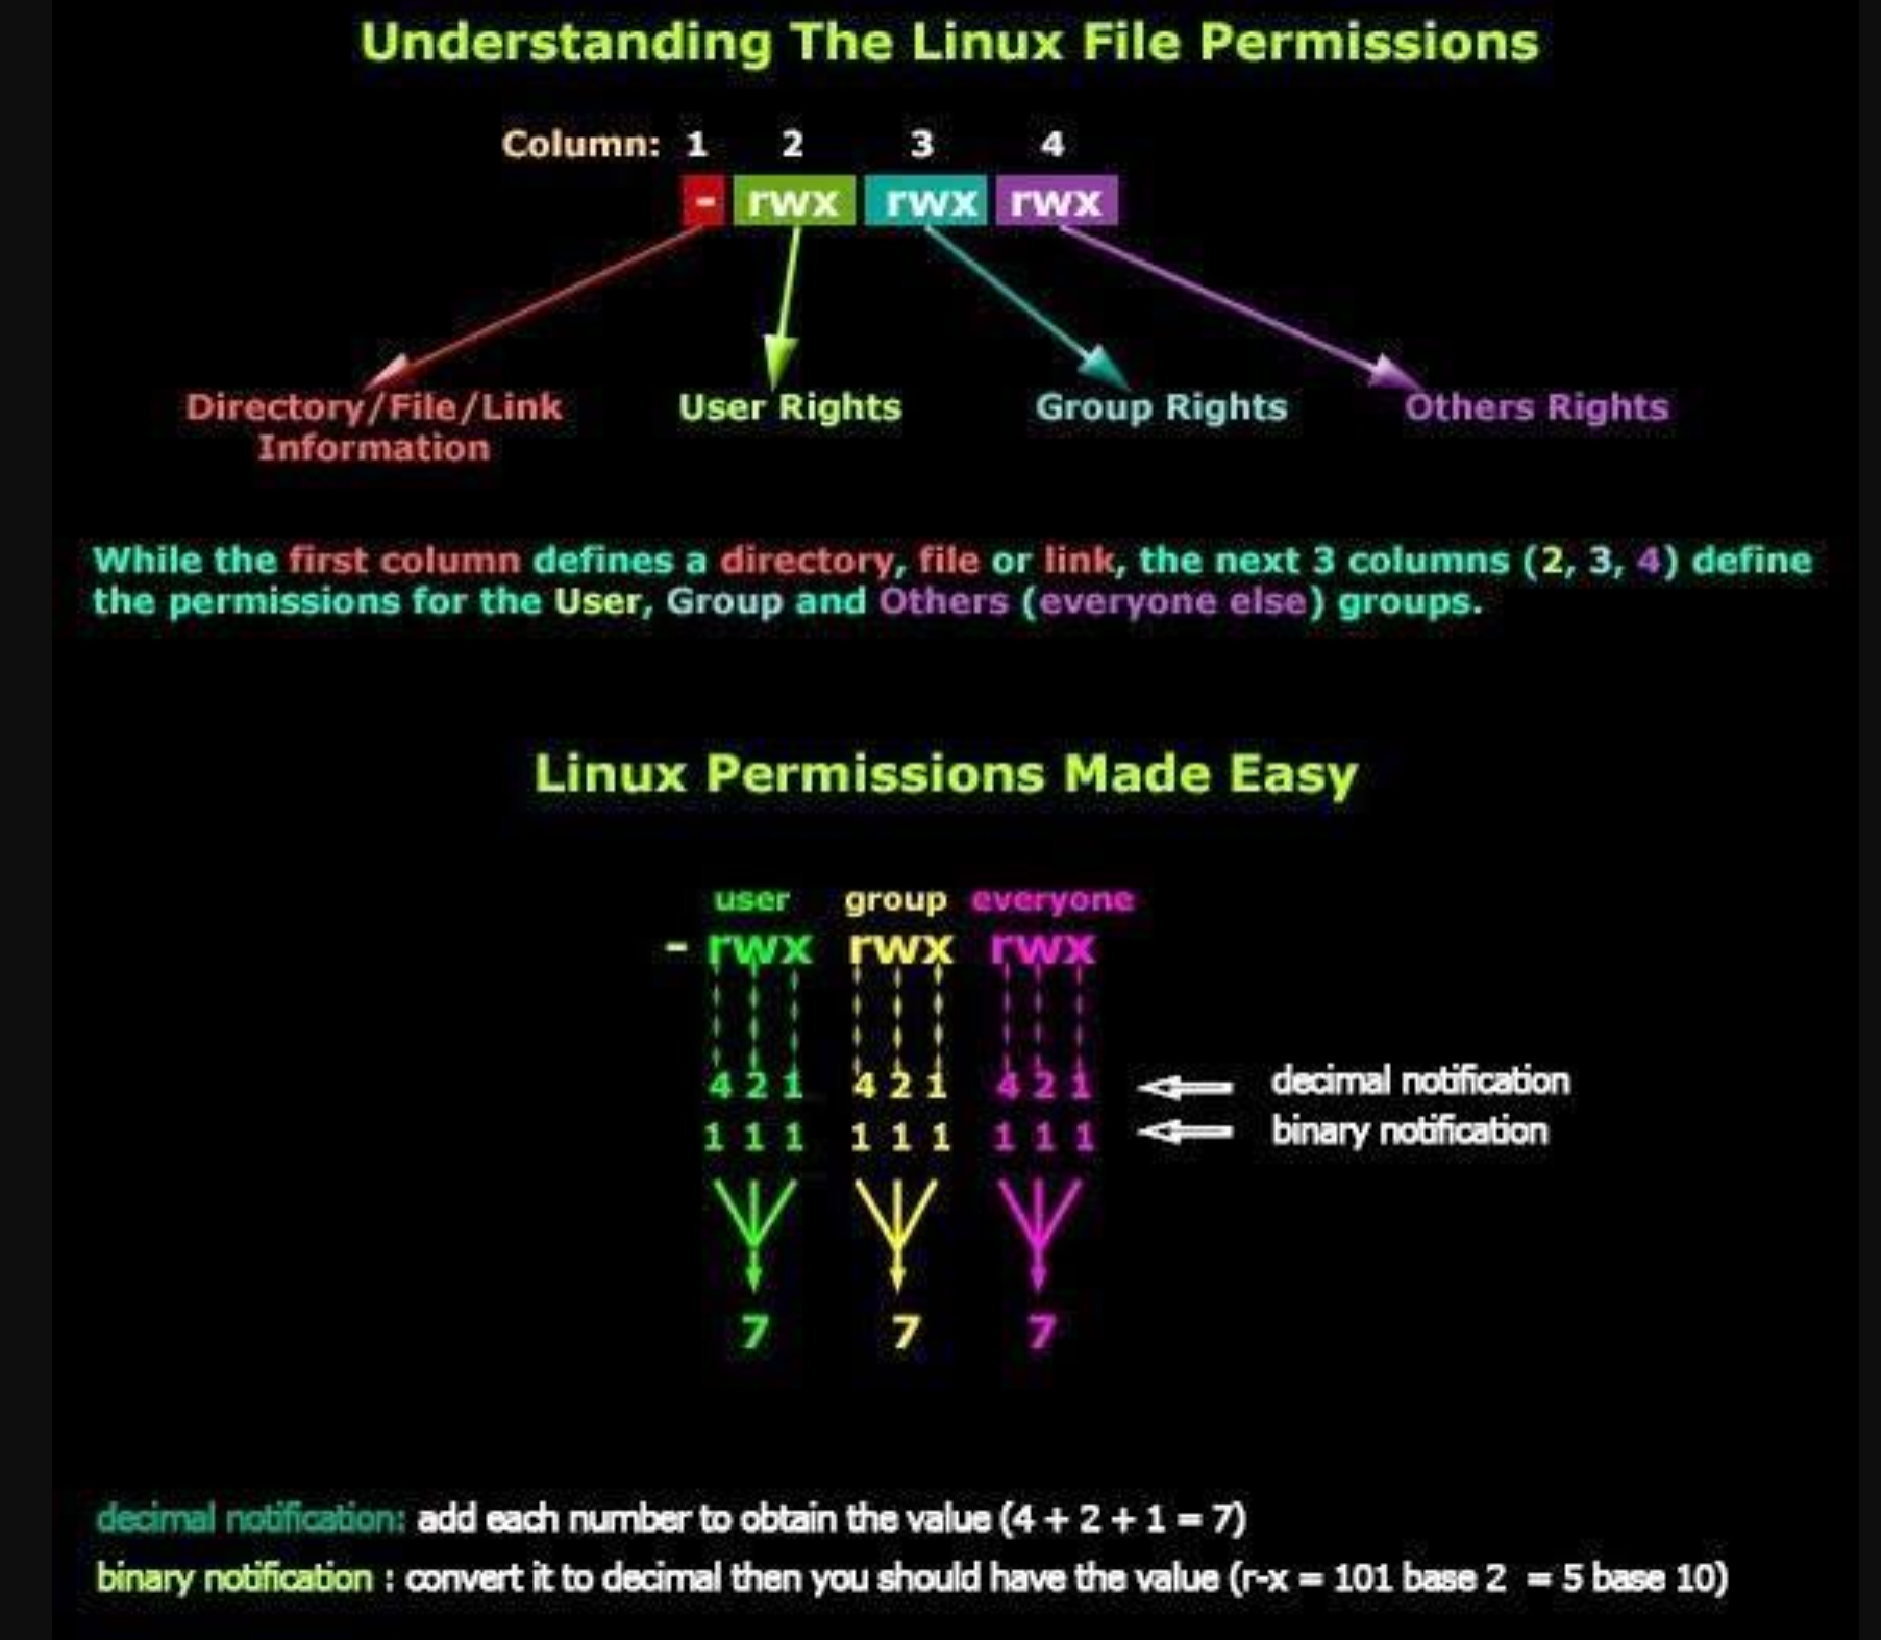
\includegraphics{figs/permissions.pdf}

Permissions can be changed with the \texttt{chmod} command. We will talk in class about
how to use it with the octal representation of permissions.

\hypertarget{editing-text-files-at-the-terminal}{%
\subsection{Editing text files at the terminal}\label{editing-text-files-at-the-terminal}}

Sometimes you might need to edit text files at the command line.

The easiest text editor to use on the command line is \texttt{nano}.
Try typing \texttt{nano\ a-file.txt} and type a few things. It is
pretty self explanatory.

\hypertarget{unix-env}{%
\section{Customizing your Environment}\label{unix-env}}

Previously we saw how to modify your command prompt to tell you what the current
working directory is (remember \texttt{PS1=\textquotesingle{}{[}\textbackslash{}W{]}-\/-\%\ \textquotesingle{}}). The limitation of giving that
command on the command line is that if you logout and then log back in again, or open
a new Terminal window, you will have to reissue that command in order to achieve
the desired look of your command prompt. Quite often a Unix user would like to make
a number of customization to the look, feel, and behavior of their Unix shell.
The bash shell allows these customization to be specified in two different files that
are read by the system so as to invoke the customization. The two files are hidden files
in the home directory: \texttt{\textasciitilde{}/.bashrc} and \texttt{\textasciitilde{}/.bash\_profile}. They are used by the Unix system
in two slightly different contexts, but for most purposes, you, the user, will not need or
even want to distinguish between the different contexts. Managing two separate files
of customization is unnecessary and requires duplication of your efforts, and can lead to inconsistent
and confusing results, so here is what we will do:

\begin{enumerate}
\def\labelenumi{\arabic{enumi}.}
\tightlist
\item
  Keep all of our customization in \texttt{\textasciitilde{}/.bashrc}.
\item
  Insert commands in \texttt{\textasciitilde{}/.bash\_profile} that say, "Hey computer! If you are looking
  for customization in here, don't bother, just get them straight out of \texttt{\textasciitilde{}/.bashrc}.
\end{enumerate}

We take care of \#2, by creating the file \texttt{\textasciitilde{}/.bash\_profile} to have the following
lines in it:

\begin{Shaded}
\begin{Highlighting}[]

\KeywordTok{if}\BuiltInTok{ [} \OtherTok{-f}\NormalTok{ ~/.bashrc}\BuiltInTok{ ]}\NormalTok{; }\KeywordTok{then}
    \BuiltInTok{source}\NormalTok{ ~/.bashrc}
\KeywordTok{fi}
\end{Highlighting}
\end{Shaded}

Taking care of \#1 is now just a matter of writing commands into \texttt{\textasciitilde{}/.bashrc}. In the following
are some recommended customization.

\hypertarget{appearances-matter}{%
\subsection{Appearances matter}\label{appearances-matter}}

Some customization just change the way your shell looks or what type of output
is given from different commands. Here are some lines to add to your \texttt{\textasciitilde{}/.bashrc}
along with some discussion of each.

\begin{Shaded}
\begin{Highlighting}[]
\BuiltInTok{export} \VariableTok{PS1=}\StringTok{'[\textbackslash{}W]--% '}
\end{Highlighting}
\end{Shaded}

This gives a tidier and more informative command prompt. The \texttt{export} command before
it tells the system to pass the value of this \emph{environment variable}, \texttt{PS1}, along
to any other shells that get spawned by the current one.

\begin{Shaded}
\begin{Highlighting}[]
\BuiltInTok{alias}\NormalTok{ ls=}\StringTok{'ls -GFh'}
\end{Highlighting}
\end{Shaded}

This makes it so that each time you invoke the \texttt{ls} command, you do so with the
options \texttt{-G}, \texttt{-F}, and \texttt{-h}. To find out on your own what those options do, you can
type \texttt{man\ ls} at the command line and read the output, but briefly: \texttt{-G} causes directories and
different file types to be printed in different colors, \texttt{-F} causes a \texttt{/} to be printed after
directory names, and other characters to be printed at the end of the names of different
file types, and \texttt{-h} causes file sizes to be printed in an easily human-readable form when
using the \texttt{-l} option.

\hypertarget{where-are-my-programscommands-at}{%
\subsection{Where are my programs/commands at?!}\label{where-are-my-programscommands-at}}

We saw in Section \ref{anatomy-command} that bash searches the directories listed in the
\texttt{PATH} variable to find commands and executables. You can modify the PATH variable to include
directories where you have installed different programs. In doing so, you want to make sure
that you don't lose any of the other directories in \texttt{PATH}, so there is a certain way to
go about redefining \texttt{PATH}. If you want to add the path \texttt{/a-new/program/directory} to your
PATH variable you do it like this:

\begin{Shaded}
\begin{Highlighting}[]
\VariableTok{PATH=$PATH}\NormalTok{:/a-new/program/directory}
\end{Highlighting}
\end{Shaded}

\hypertarget{a-few-more-important-keystrokes}{%
\section{A Few More Important Keystrokes}\label{a-few-more-important-keystrokes}}

If a command ``gets stuck'' or is running longer than it should be, you can usually
kill/quit it by doing \texttt{cntrl-c}.

Once you have given a command, it gets stored in your bash history. You can use the
up-arrow key to cycle backward through different commands in your history. This is particularly
useful if you are building up complex pipelines on the command line piece by piece, looking at
the output of each to make sure it is correct. Rather than re-typing what you did for the last
command line, you just up-arrow it.

Once you have done an up-arrow or two, you can cycle back down through your history with
a down-arrow.

Finally, you can search through your bash history by typing \texttt{cntrl-r} and then typing
the word/command you are looking for. For example, if, 100 command lines back, you
used a command that involved the program \texttt{awk}, you can search for that by typing
\texttt{cntrl-r} and then typing \texttt{awk}.

One last big thing to note: the \texttt{\#} is considered a \emph{comment character} in bash.
This means that any text following a \texttt{\#} (unless it is backslash-escaped or inside quotation marks),
until the next line ending,
will be ignored by the shell.

\hypertarget{a-short-list-of-additional-useful-commands.}{%
\section{A short list of additional useful commands.}\label{a-short-list-of-additional-useful-commands.}}

Everyone should be familiar with the following commands, and the
options that follow them on each line below. One might even think of
scanning the manual page for each of these:

\begin{itemize}
\tightlist
\item
  \texttt{echo}
\item
  \texttt{cat}
\item
  \texttt{head}, \texttt{-n,\ -c}
\item
  \texttt{tail}, \texttt{-n}
\item
  \texttt{less}
\item
  \texttt{sort}, \texttt{-n\ -b\ -k}
\item
  \texttt{paste}
\item
  \texttt{cut}, \texttt{-d}
\item
  \texttt{tar}, \texttt{-cvf,\ -xvf}
\item
  \texttt{gzip}, \texttt{-c}
\item
  \texttt{du}, \texttt{-h\ -C},
\item
  \texttt{wc}
\item
  \texttt{date}
\item
  \texttt{uniq}
\item
  \texttt{chmod}, \texttt{u+x}, \texttt{ug+x}
\item
  \texttt{grep}
\end{itemize}

\hypertarget{two-important-computing-concepts}{%
\section{Two important computing concepts}\label{two-important-computing-concepts}}

\hypertarget{compression}{%
\subsection{Compression}\label{compression}}

Most file storage types (like text files) are a bit wasteful in terms of
file space: every character in a text file takes the same number of bytes to
store, whether it is a character that is used a lot, like \texttt{s} or \texttt{e}, or whether
it is a character that is seldom seen in many text files, like \texttt{\^{}}. \emph{Compression}
is the art of creating a code for different types of data that uses fewer bits to
encode ``letters'' (or ``chunks'' of data) that occur frequently and it reserves codewords of
more bits to encode less frequently occurring chunks in the data. The result is that the
total file size is smaller than the uncompressed version. However, in order to read it,
the file must be decompressed.

In bioinformatics, many of the files you deal with will be compressed, because that
can save many terabytes of disk space. Most often, files will be compressed using the
\texttt{gzip} utility, and they can be uncompressed with the \texttt{gunzip} command. Sometimes
you might want to just look at the fist part of a compressed file. If the file is compressed
with \texttt{gzip}, you can decompress to \emph{stdout} by using \texttt{gzcat} and then pipe it to \texttt{head}, for example.

A central form of compression in bioinformatics is called \texttt{bgzip} compression
which compresses files into a series of blocks of the same size, situated in such a way that
it is possible to \emph{index} the contents of the file so that certain parts of the file can be
accessed without decompressing the whole thing. We will encounter indexed compressed files a
lot when we start dealing with BAM and vcf.gz files.

\hypertarget{hashing}{%
\subsection{Hashing}\label{hashing}}

The final topic we will cover here is the topic of hashing, an in particular
the idea of ``fingerprinting'' files on ones computer. This process is central
to how the git version control system works, and it is well worth knowing about.

Any file on your computer can be thought of as a series of bits, 0's and 1's, as,
fundamentally, that is what the file is. A \emph{hashing algorithm} is an algorithm
that maps a series of bits (or arbitrary length) to a short sequence of bits. The
SHA1 hashing algorithm maps arbitrary sequences of bits to a sequence of 160 bits.

There are \(2^{160} \approx 1.46 \times 10^{48}\) possible bit sequences of length 160.
That is a vast number. If your hashing algorithm is well randomized, so that bit sequences
are hashed into 160 bits in a roughly uniform distribution, then it is exceedingly unlikely
that any two bit sequences (i.e.~files on your filesystem) will have the same hash (``fingerprint'')
unless they are perfectly identical. As hashing algorithms are often quite fast to compute,
this provides an exceptionally good way to verify that two files are identical.

The SHA1 algorithm is implemented with the \texttt{shasum} command. In the following,
as a demonstration, I store the recursive listing of my \texttt{git-repos} directory into
a file and I hash it. Then I add just a single line ending to the end
of the file, and hash that, to note that the two hashes are not at all similar
even though the two files differ by only one character:

\begin{Shaded}
\begin{Highlighting}[]
\NormalTok{[}\ExtensionTok{~}\NormalTok{]}\ExtensionTok{--%}\NormalTok{ ls -R Documents/git-repos/* }\OperatorTok{>}\NormalTok{ /tmp/gr-list.txt }
\NormalTok{[}\ExtensionTok{~}\NormalTok{]}\ExtensionTok{--%} \CommentTok{# how many lines is that?}
\NormalTok{[}\ExtensionTok{~}\NormalTok{]}\ExtensionTok{--%}\NormalTok{ wc /tmp/gr-list.txt }
   \ExtensionTok{93096}\NormalTok{   88177 2310967 /tmp/gr-list.txt}
\NormalTok{[}\ExtensionTok{~}\NormalTok{]}\ExtensionTok{--%}\NormalTok{ shasum /tmp/gr-list.txt }
\ExtensionTok{1396f2fec4eebdee079830e1eff9e3a64ba5588c}\NormalTok{  /tmp/gr-list.txt}
\NormalTok{[}\ExtensionTok{~}\NormalTok{]}\ExtensionTok{--%} \CommentTok{# now add a line ending to the end}
\NormalTok{[}\ExtensionTok{~}\NormalTok{]}\ExtensionTok{--%}\NormalTok{ (cat /tmp/gr-list.txt}\KeywordTok{;} \BuiltInTok{echo}\NormalTok{) }\OperatorTok{>} \ExtensionTok{/tmp/gr-list2.txt} 
\NormalTok{[}\ExtensionTok{~}\NormalTok{]}\ExtensionTok{--%} \CommentTok{# hash both and compare}
\NormalTok{[}\ExtensionTok{~}\NormalTok{]}\ExtensionTok{--%}\NormalTok{ shasum /tmp/gr-list.txt /tmp/gr-list2.txt }
\ExtensionTok{1396f2fec4eebdee079830e1eff9e3a64ba5588c}\NormalTok{  /tmp/gr-list.txt}
\ExtensionTok{23bff8776ff86e5ebbe39e11cc2f5e31c286ae91}\NormalTok{  /tmp/gr-list2.txt}
\NormalTok{[}\ExtensionTok{~}\NormalTok{]}\ExtensionTok{--%} \CommentTok{# whoa! cool.}
\end{Highlighting}
\end{Shaded}

\hypertarget{unix-quick-study-guide}{%
\section{Unix: Quick Study Guide}\label{unix-quick-study-guide}}

This is just a table with quick topics/commands/words in it. You should
understand each and be able to tell a friend a lot about each one. Cite it
as \ref{tab:unix-chap-review}

\begin{longtable}[]{@{}lll@{}}
\caption{\label{tab:unix-chap-review} Terms/ideas/etc. to know forward and backward}\tabularnewline
\toprule
\endhead
\begin{minipage}[t]{0.34\columnwidth}\raggedright
bash\strut
\end{minipage} & \begin{minipage}[t]{0.35\columnwidth}\raggedright
absolute path\strut
\end{minipage} & \begin{minipage}[t]{0.22\columnwidth}\raggedright
relative path\strut
\end{minipage}\tabularnewline
\begin{minipage}[t]{0.34\columnwidth}\raggedright
\texttt{/} at beginning of path\strut
\end{minipage} & \begin{minipage}[t]{0.35\columnwidth}\raggedright
\texttt{/} between directories\strut
\end{minipage} & \begin{minipage}[t]{0.22\columnwidth}\raggedright
home directory\strut
\end{minipage}\tabularnewline
\begin{minipage}[t]{0.34\columnwidth}\raggedright
\texttt{\textasciitilde{}}\strut
\end{minipage} & \begin{minipage}[t]{0.35\columnwidth}\raggedright
current working directory\strut
\end{minipage} & \begin{minipage}[t]{0.22\columnwidth}\raggedright
\texttt{pwd}\strut
\end{minipage}\tabularnewline
\begin{minipage}[t]{0.34\columnwidth}\raggedright
\texttt{cd}\strut
\end{minipage} & \begin{minipage}[t]{0.35\columnwidth}\raggedright
\texttt{.}\strut
\end{minipage} & \begin{minipage}[t]{0.22\columnwidth}\raggedright
\texttt{..}\strut
\end{minipage}\tabularnewline
\begin{minipage}[t]{0.34\columnwidth}\raggedright
\texttt{cd\ -}\strut
\end{minipage} & \begin{minipage}[t]{0.35\columnwidth}\raggedright
basename\strut
\end{minipage} & \begin{minipage}[t]{0.22\columnwidth}\raggedright
PS1\strut
\end{minipage}\tabularnewline
\begin{minipage}[t]{0.34\columnwidth}\raggedright
TAB-completion\strut
\end{minipage} & \begin{minipage}[t]{0.35\columnwidth}\raggedright
\texttt{ls} (\texttt{-a}, \texttt{-d}, \texttt{-R})\strut
\end{minipage} & \begin{minipage}[t]{0.22\columnwidth}\raggedright
globbing\strut
\end{minipage}\tabularnewline
\begin{minipage}[t]{0.34\columnwidth}\raggedright
*\strut
\end{minipage} & \begin{minipage}[t]{0.35\columnwidth}\raggedright
?\strut
\end{minipage} & \begin{minipage}[t]{0.22\columnwidth}\raggedright
{[}0-9{]}\strut
\end{minipage}\tabularnewline
\begin{minipage}[t]{0.34\columnwidth}\raggedright
{[}a-z{]}\strut
\end{minipage} & \begin{minipage}[t]{0.35\columnwidth}\raggedright
{[}\^{}CDcd{]}\strut
\end{minipage} & \begin{minipage}[t]{0.22\columnwidth}\raggedright
\{png,jpg,pdf\}\strut
\end{minipage}\tabularnewline
\begin{minipage}[t]{0.34\columnwidth}\raggedright
\texttt{echo}\strut
\end{minipage} & \begin{minipage}[t]{0.35\columnwidth}\raggedright
\texttt{man} \emph{command}\strut
\end{minipage} & \begin{minipage}[t]{0.22\columnwidth}\raggedright
\texttt{mkdir}\strut
\end{minipage}\tabularnewline
\begin{minipage}[t]{0.34\columnwidth}\raggedright
\texttt{mv}\strut
\end{minipage} & \begin{minipage}[t]{0.35\columnwidth}\raggedright
\texttt{cp}\strut
\end{minipage} & \begin{minipage}[t]{0.22\columnwidth}\raggedright
\texttt{rm}\strut
\end{minipage}\tabularnewline
\begin{minipage}[t]{0.34\columnwidth}\raggedright
\texttt{cat}\strut
\end{minipage} & \begin{minipage}[t]{0.35\columnwidth}\raggedright
\texttt{head}\strut
\end{minipage} & \begin{minipage}[t]{0.22\columnwidth}\raggedright
\texttt{less}\strut
\end{minipage}\tabularnewline
\begin{minipage}[t]{0.34\columnwidth}\raggedright
\emph{stdout}\strut
\end{minipage} & \begin{minipage}[t]{0.35\columnwidth}\raggedright
\emph{stdin}\strut
\end{minipage} & \begin{minipage}[t]{0.22\columnwidth}\raggedright
\emph{stderr}\strut
\end{minipage}\tabularnewline
\begin{minipage}[t]{0.34\columnwidth}\raggedright
\texttt{\textgreater{}}\strut
\end{minipage} & \begin{minipage}[t]{0.35\columnwidth}\raggedright
\texttt{\textless{}}\strut
\end{minipage} & \begin{minipage}[t]{0.22\columnwidth}\raggedright
\texttt{\textbar{}}\strut
\end{minipage}\tabularnewline
\begin{minipage}[t]{0.34\columnwidth}\raggedright
\texttt{ln\ -s}\strut
\end{minipage} & \begin{minipage}[t]{0.35\columnwidth}\raggedright
symbolic link\strut
\end{minipage} & \begin{minipage}[t]{0.22\columnwidth}\raggedright
PATH\strut
\end{minipage}\tabularnewline
\begin{minipage}[t]{0.34\columnwidth}\raggedright
\texttt{-rw-r-\/-r-\/-}\strut
\end{minipage} & \begin{minipage}[t]{0.35\columnwidth}\raggedright
.bashrc\strut
\end{minipage} & \begin{minipage}[t]{0.22\columnwidth}\raggedright
.bash\_profile\strut
\end{minipage}\tabularnewline
\begin{minipage}[t]{0.34\columnwidth}\raggedright
\texttt{sort}, \texttt{-n\ -b\ -k}\strut
\end{minipage} & \begin{minipage}[t]{0.35\columnwidth}\raggedright
\texttt{paste}\strut
\end{minipage} & \begin{minipage}[t]{0.22\columnwidth}\raggedright
\texttt{cut}, \texttt{-d}\strut
\end{minipage}\tabularnewline
\begin{minipage}[t]{0.34\columnwidth}\raggedright
\texttt{tar}, \texttt{-cvf,\ -xvf}\strut
\end{minipage} & \begin{minipage}[t]{0.35\columnwidth}\raggedright
\texttt{gzip}\strut
\end{minipage} & \begin{minipage}[t]{0.22\columnwidth}\raggedright
\texttt{du}, \texttt{-h\ -C},\strut
\end{minipage}\tabularnewline
\begin{minipage}[t]{0.34\columnwidth}\raggedright
\texttt{wc}\strut
\end{minipage} & \begin{minipage}[t]{0.35\columnwidth}\raggedright
\texttt{date}\strut
\end{minipage} & \begin{minipage}[t]{0.22\columnwidth}\raggedright
\texttt{uniq}\strut
\end{minipage}\tabularnewline
\begin{minipage}[t]{0.34\columnwidth}\raggedright
cntrl-c\strut
\end{minipage} & \begin{minipage}[t]{0.35\columnwidth}\raggedright
cntrl-r\strut
\end{minipage} & \begin{minipage}[t]{0.22\columnwidth}\raggedright
\texttt{\#}\strut
\end{minipage}\tabularnewline
\begin{minipage}[t]{0.34\columnwidth}\raggedright
up-arrow/down-arrow\strut
\end{minipage} & \begin{minipage}[t]{0.35\columnwidth}\raggedright
\texttt{chmod}, \texttt{ug+x}, \texttt{664}\strut
\end{minipage} & \begin{minipage}[t]{0.22\columnwidth}\raggedright
\texttt{grep}\strut
\end{minipage}\tabularnewline
\bottomrule
\end{longtable}

\hypertarget{shell-programming}{%
\chapter{Shell programming}\label{shell-programming}}

In our first foray into Unix and the shell, we restricted ourselves mostly
to navigating the file system, handling files, and working with streams of data
(via redirection and pipes). These are all crucial skills, but the bash shell
becomes truly powerful when we start to adopt it as a sort of programming language.
That's right, even though the functionality of bash is geared toward running jobs
and calling commands, it still exhibits most of the features expected in a programming
language, like variables, iteration and flow control.

\hypertarget{an-example-script}{%
\section{An example script}\label{an-example-script}}

We start this chapter by taking a look at a short bash program (typically
called a \emph{script}) that the author wrote in order to efficiently download
(clone, really) repositories from GitHub that have been submitted by
students to GitHub Classroom. The program is not long, but exhibits
many useful features of bash as a programming language. If you are reading
this, not in the context of a class with lectures, just go ahead and read
through it and see if you can figure out what is going on in each line
of the script. Afterward, we will address many features of bash by
referencing different parts of the script.

The script, which happens to be stored in a file called \texttt{clone-classroom-repos.sh}
is printed below, with linenumbers, since we will
be referring back to specific sections of the script later.

\begin{Shaded}
\begin{Highlighting}[numbers=left,,]
\CommentTok{#!/bin/bash}

\CommentTok{# define a function to print the usage or "help" for the script}
\KeywordTok{function}\FunctionTok{ usage} \KeywordTok{\{}
      \BuiltInTok{echo}\NormalTok{ Syntax:}
      \BuiltInTok{echo} \StringTok{"  }\VariableTok{$(}\FunctionTok{basename} \VariableTok{$0)}\StringTok{  GH_Prefix  Repo_Prefix  Branch  Dir}
\StringTok{      }
\StringTok{      GH_Prefix: the URL of the GitHub site where the repository exists.}
\StringTok{      Repo_Prefix: the prefix of the name of each repository to be cloned.}
\StringTok{      Branch: the name of the branch to create and switch to in the repository,}
\StringTok{         once the repo has been cloned.}
\StringTok{      Dir: path to the directory (will be created if necessary) to clone all}
\StringTok{         the repositories to.}
\StringTok{         }
\StringTok{   Example:}
\StringTok{   }
\StringTok{      }\VariableTok{$(}\FunctionTok{basename} \VariableTok{$0)}\StringTok{  https://github.com/CSU-con-gen-bioinformatics-2020  illumina-video-questions- erics-edits  /tmp/illumina-questions}
\StringTok{      "}
      \BuiltInTok{echo}
\KeywordTok{\}}

\CommentTok{#  test for right number of required args.  If not, print usage message}
\KeywordTok{if}\BuiltInTok{ [} \VariableTok{$#} \OtherTok{-ne}\NormalTok{ 4}\BuiltInTok{ ]}\NormalTok{; }\KeywordTok{then}
    \ExtensionTok{usage}\KeywordTok{;}
    \BuiltInTok{exit}\NormalTok{ 1}\KeywordTok{;}
\KeywordTok{fi}

\CommentTok{# copy positional parameters into other variables}
\VariableTok{GHP=$1}
\VariableTok{RP=$2}
\VariableTok{BRANCH=$3}
\VariableTok{DD=$4}

\CommentTok{# assign string with student GitHub handles into a variable}
\VariableTok{GHNAMES=}\StringTok{"AmandaCicchino}
\StringTok{BrennaF}
\StringTok{CaitlinWells}
\StringTok{EllenMCampbell}
\StringTok{FayDong}
\StringTok{LibbyGH}
\StringTok{NathanPhipps}
\StringTok{RGCheek}
\StringTok{Ronan17}
\StringTok{abeulke}
\StringTok{carolazari}
\StringTok{cbossu}
\StringTok{ccolumbu}
\StringTok{elenacorrea}
\StringTok{eriqande}
\StringTok{jenleon07}
\StringTok{kimhoke}
\StringTok{kruegg}
\StringTok{lauracgoetz}
\StringTok{mdrod110}
\StringTok{mgdesaix}
\StringTok{raven-wings}
\StringTok{seamus100}
\StringTok{taylorbobowski}
\StringTok{wcfunk"}

\CommentTok{# assign my GitHub username to the variable USER}
\VariableTok{USER=}\NormalTok{eriqande}

\CommentTok{# assign the current working directory to the variable RUNDIR}
\VariableTok{RUNDIR=$PWD}

\CommentTok{# make a new directory named whatever the user wanted for the output directory}
\FunctionTok{mkdir}\NormalTok{ -p }\VariableTok{$DD}

\CommentTok{# make variables to hold log and error file names}
\VariableTok{LOG=$\{PWD\}}\NormalTok{/}\VariableTok{$\{RP\}}\NormalTok{log}
\VariableTok{ERR=$LOG}\NormalTok{.stderr}

\CommentTok{# print the date/time when the process is starting}
\BuiltInTok{echo} \StringTok{"STARTING at }\VariableTok{$(}\FunctionTok{date}\VariableTok{)}\StringTok{"}

\CommentTok{# make a clean slate. remove any files with the name}
\CommentTok{# of the error output file}
\FunctionTok{rm}\NormalTok{ -f }\VariableTok{$ERR}

\CommentTok{# cycle over the student GitHub names, and for each one *do*}
\CommentTok{# the commands that appear before the *done* keyword. Indenting}
\CommentTok{# is used to make it easier to read, but is not essential.}
\KeywordTok{for} \ExtensionTok{L}\NormalTok{ in }\VariableTok{$GHNAMES}\KeywordTok{;} \KeywordTok{do}

    \BuiltInTok{echo} \StringTok{"Working on }\VariableTok{$L}\StringTok{, starting at }\VariableTok{$(}\FunctionTok{date}\VariableTok{)}\StringTok{"}\NormalTok{  # print a progress line to stdout}
    \VariableTok{REPO=$GHP}\NormalTok{/}\VariableTok{$\{RP\}$L}\NormalTok{     # }\ExtensionTok{combine}\NormalTok{ variables into new variables that}
    \BuiltInTok{echo} \VariableTok{$REPO}\NormalTok{            # hold the URL for the repository to be}
    \VariableTok{DEST=$DD}\NormalTok{/}\VariableTok{$L}\NormalTok{           # }\ExtensionTok{cloned}\NormalTok{ and the path where it should be cloned to}
  
    \CommentTok{# store the commands themselves into variables. Note the }
    \CommentTok{# use of double quotes.}
    \VariableTok{CLONE_IT=}\StringTok{"git clone }\VariableTok{$\{REPO/}\NormalTok{github.com}\VariableTok{/$USER}\NormalTok{@github.com}\VariableTok{\}}\StringTok{ }\VariableTok{$DEST}\StringTok{"} 
    \VariableTok{BRANCH_IT=}\StringTok{"git checkout -B }\VariableTok{$BRANCH}\StringTok{"}
    \VariableTok{PUSH_IT=}\StringTok{"git push -u origin }\VariableTok{$BRANCH}\StringTok{"}
  
    
    \CommentTok{# now, run those commands, chained together by exit-status-AND}
    \CommentTok{# operators (so it will stop if any one part fails), while}
    \CommentTok{# all the while appending error statements to the Error file. Run it}
    \CommentTok{# all within an "if" statement so you can deliver a report as to}
    \CommentTok{# whether the whole shebang succeeded or failed.}
    \KeywordTok{if} \VariableTok{$CLONE_IT} \OperatorTok{2>>} \VariableTok{$ERR}  \KeywordTok{&&} \KeywordTok{\textbackslash{}}
        \BuiltInTok{cd} \VariableTok{$DEST} \KeywordTok{&&} \KeywordTok{\textbackslash{}}
        \VariableTok{$BRANCH_IT} \OperatorTok{2>>} \VariableTok{$ERR}  \KeywordTok{&&} \KeywordTok{\textbackslash{}}
        \VariableTok{$PUSH_IT} \OperatorTok{2>>} \VariableTok{$ERR}  \KeywordTok{&&} \KeywordTok{\textbackslash{}}
        \BuiltInTok{cd} \VariableTok{$RUNDIR}\NormalTok{   # at the very end make sure to return to the original working directory}
    \KeywordTok{then}
        \BuiltInTok{echo} \StringTok{"FULL SUCCESS }\VariableTok{$L}\StringTok{"}
    \KeywordTok{else}
        \BuiltInTok{echo} \StringTok{"FAILURE SOMEWHERE WITHIN }\VariableTok{$L}\StringTok{"}
        \BuiltInTok{cd} \VariableTok{$RUNDIR}\NormalTok{  # get back to the working directory from which the original command was run.}
                    \CommentTok{# so we are ready to handle the next student repo.}
    \KeywordTok{fi}
  
\KeywordTok{done}\NormalTok{  # }\ExtensionTok{signifies}\NormalTok{ the end of the for loop we are cycling over}
\end{Highlighting}
\end{Shaded}

If my current working directory is where the script resides, I can run it
like this:

\begin{Shaded}
\begin{Highlighting}[]
\ExtensionTok\NormalTok{ clone-classroom-repos.sh }
\end{Highlighting}
\end{Shaded}

from anywhere on my computer.

When I run the script in any of those two ways, because I have not provided the
proper number of \emph{arguments} to the command, it returns a message telling me
what syntax is required to use it (i.e., its \emph{usage syntax}):

\begin{Shaded}
\begin{Highlighting}[]
\ExtensionTok{%}\NormalTok{ clone-classroom-repos.sh }
\ExtensionTok{Syntax}\NormalTok{:}
  \ExtensionTok{clone-classroom-repos.sh}\NormalTok{  GH_Prefix  Repo_Prefix  Branch  Dir}
      
      \ExtensionTok{GH_Prefix}\NormalTok{: the URL of the GitHub site where the repository exists.}
      \ExtensionTok{Repo_Prefix}\NormalTok{: the prefix of the name of each repository to be cloned.}
      \ExtensionTok{Branch}\NormalTok{: the name of the branch to create and switch to in the repository,}
         \ExtensionTok{once}\NormalTok{ the repo has been cloned.}
      \ExtensionTok{Dir}\NormalTok{: path to the directory (will be created if necessary) }\ExtensionTok{to}\NormalTok{ clone all}
         \ExtensionTok{the}\NormalTok{ repositories to.}
         
   \ExtensionTok{Example}\NormalTok{:}
   
      \ExtensionTok{clone-classroom-repos.sh}\NormalTok{  https://github.com/CSU-con-gen-bioinformatics-2020  illumina-video-questions- erics-edits  /tmp/illumina-questions}
      
\end{Highlighting}
\end{Shaded}

That is handy, and the code to do it exists in the script itself. Looking at the output, how many
arguments do you think the script is expecting?

Now, if I wanted to clone all of the student GitHub repos associated with the \texttt{illumina-video-questions}
homework set, and then, once cloned, set up a new git \emph{branch} called \texttt{eric-edits} so that I can make
edits and/or comments and send those to students via a pull request, here is the command I would give
(remembering, again that the \texttt{\%} signifies the command prompt, here):

\begin{Shaded}
\begin{Highlighting}[]
\ExtensionTok{%}\NormalTok{ clone-classroom-repos.sh  https://github.com/CSU-con-gen-bioinformatics-2020  illumina-video-questions- erics-edits  /tmp/illumina-questions}
\end{Highlighting}
\end{Shaded}

And when I do, I see output like this:

\begin{verbatim}
STARTING at Thu Feb 13 06:02:05 MST 2020
Working on AmandaCicchino, starting at Thu Feb 13 06:02:05 MST 2020
https://github.com/CSU-con-gen-bioinformatics-2020/illumina-video-questions-AmandaCicchino
Branch erics-edits set up to track remote branch erics-edits from origin.
FULL SUCCESS AmandaCicchino
Working on BrennaF, starting at Thu Feb 13 06:02:07 MST 2020
https://github.com/CSU-con-gen-bioinformatics-2020/illumina-video-questions-BrennaF
Branch erics-edits set up to track remote branch erics-edits from origin.
FULL SUCCESS BrennaF
Working on CaitlinWells, starting at Thu Feb 13 06:02:08 MST 2020
https://github.com/CSU-con-gen-bioinformatics-2020/illumina-video-questions-CaitlinWells
FAILURE SOMEWHERE WITHIN CaitlinWells
Working on EllenMCampbell, starting at Thu Feb 13 06:02:09 MST 2020
https://github.com/CSU-con-gen-bioinformatics-2020/illumina-video-questions-EllenMCampbell
Branch erics-edits set up to track remote branch erics-edits from origin.
FULL SUCCESS EllenMCampbell
Working on FayDong, starting at Thu Feb 13 06:02:10 MST 2020
https://github.com/CSU-con-gen-bioinformatics-2020/illumina-video-questions-FayDong
Branch erics-edits set up to track remote branch erics-edits from origin.
FULL SUCCESS FayDong
Working on LibbyGH, starting at Thu Feb 13 06:02:12 MST 2020
https://github.com/CSU-con-gen-bioinformatics-2020/illumina-video-questions-LibbyGH
Branch erics-edits set up to track remote branch erics-edits from origin.
FULL SUCCESS LibbyGH
Working on NathanPhipps, starting at Thu Feb 13 06:02:14 MST 2020
https://github.com/CSU-con-gen-bioinformatics-2020/illumina-video-questions-NathanPhipps
Branch erics-edits set up to track remote branch erics-edits from origin.
FULL SUCCESS NathanPhipps
Working on RGCheek, starting at Thu Feb 13 06:02:15 MST 2020
https://github.com/CSU-con-gen-bioinformatics-2020/illumina-video-questions-RGCheek
Branch erics-edits set up to track remote branch erics-edits from origin.
FULL SUCCESS RGCheek
Working on Ronan17, starting at Thu Feb 13 06:02:17 MST 2020
https://github.com/CSU-con-gen-bioinformatics-2020/illumina-video-questions-Ronan17
Branch erics-edits set up to track remote branch erics-edits from origin.
FULL SUCCESS Ronan17
Working on abeulke, starting at Thu Feb 13 06:02:19 MST 2020
https://github.com/CSU-con-gen-bioinformatics-2020/illumina-video-questions-abeulke
Branch erics-edits set up to track remote branch erics-edits from origin.
FULL SUCCESS abeulke
Working on carolazari, starting at Thu Feb 13 06:02:21 MST 2020
https://github.com/CSU-con-gen-bioinformatics-2020/illumina-video-questions-carolazari
Branch erics-edits set up to track remote branch erics-edits from origin.
FULL SUCCESS carolazari
Working on cbossu, starting at Thu Feb 13 06:02:23 MST 2020
https://github.com/CSU-con-gen-bioinformatics-2020/illumina-video-questions-cbossu
Branch erics-edits set up to track remote branch erics-edits from origin.
FULL SUCCESS cbossu
Working on ccolumbu, starting at Thu Feb 13 06:02:25 MST 2020
https://github.com/CSU-con-gen-bioinformatics-2020/illumina-video-questions-ccolumbu
Branch erics-edits set up to track remote branch erics-edits from origin.
FULL SUCCESS ccolumbu
Working on elenacorrea, starting at Thu Feb 13 06:02:26 MST 2020
https://github.com/CSU-con-gen-bioinformatics-2020/illumina-video-questions-elenacorrea
Branch erics-edits set up to track remote branch erics-edits from origin.
FULL SUCCESS elenacorrea
Working on eriqande, starting at Thu Feb 13 06:02:28 MST 2020
https://github.com/CSU-con-gen-bioinformatics-2020/illumina-video-questions-eriqande
Branch erics-edits set up to track remote branch erics-edits from origin.
FULL SUCCESS eriqande
Working on jenleon07, starting at Thu Feb 13 06:02:29 MST 2020
https://github.com/CSU-con-gen-bioinformatics-2020/illumina-video-questions-jenleon07
FAILURE SOMEWHERE WITHIN jenleon07
Working on kimhoke, starting at Thu Feb 13 06:02:30 MST 2020
https://github.com/CSU-con-gen-bioinformatics-2020/illumina-video-questions-kimhoke
FAILURE SOMEWHERE WITHIN kimhoke
Working on kruegg, starting at Thu Feb 13 06:02:30 MST 2020
https://github.com/CSU-con-gen-bioinformatics-2020/illumina-video-questions-kruegg
FAILURE SOMEWHERE WITHIN kruegg
Working on lauracgoetz, starting at Thu Feb 13 06:02:30 MST 2020
https://github.com/CSU-con-gen-bioinformatics-2020/illumina-video-questions-lauracgoetz
FAILURE SOMEWHERE WITHIN lauracgoetz
Working on mdrod110, starting at Thu Feb 13 06:02:31 MST 2020
https://github.com/CSU-con-gen-bioinformatics-2020/illumina-video-questions-mdrod110
Branch erics-edits set up to track remote branch erics-edits from origin.
FULL SUCCESS mdrod110
Working on mgdesaix, starting at Thu Feb 13 06:02:32 MST 2020
https://github.com/CSU-con-gen-bioinformatics-2020/illumina-video-questions-mgdesaix
Branch erics-edits set up to track remote branch erics-edits from origin.
FULL SUCCESS mgdesaix
Working on raven-wings, starting at Thu Feb 13 06:02:34 MST 2020
https://github.com/CSU-con-gen-bioinformatics-2020/illumina-video-questions-raven-wings
FAILURE SOMEWHERE WITHIN raven-wings
Working on seamus100, starting at Thu Feb 13 06:02:34 MST 2020
https://github.com/CSU-con-gen-bioinformatics-2020/illumina-video-questions-seamus100
Branch erics-edits set up to track remote branch erics-edits from origin.
FULL SUCCESS seamus100
Working on taylorbobowski, starting at Thu Feb 13 06:02:36 MST 2020
https://github.com/CSU-con-gen-bioinformatics-2020/illumina-video-questions-taylorbobowski
Branch erics-edits set up to track remote branch erics-edits from origin.
FULL SUCCESS taylorbobowski
Working on wcfunk, starting at Thu Feb 13 06:02:37 MST 2020
https://github.com/CSU-con-gen-bioinformatics-2020/illumina-video-questions-wcfunk
Branch erics-edits set up to track remote branch erics-edits from origin.
FULL SUCCESS wcfunk
\end{verbatim}

From that report, it is clear that it takes about 1 to 2 seconds to handle each
repository. If I were doing each repository by hand, (i.e.~cloning and
branching through a GUI
interface like RStudio's) each repository would probably take me about 30 seconds
to a minute, with a lot of copying and pasting and chance for errors,
and I would have destroyed my wrists with all the repetitive tasks. So, this
is a HUGE deal.

It is also easy to scan through the results and see, ``Holy Moly! These are
some dedicated students!'' Everyone has successfully submitted their homework repositories
(and thus we were \texttt{SUCCESS}-ful in cloning them), except for a handful
who were traveling or otherwise occupied and had warned me they wouldn't
be able to do the assignment.

When all is said and done, I have the following git repositories on my laptop which
I can peruse at my leisure:

\begin{Shaded}
\begin{Highlighting}[]
\ExtensionTok{%}\NormalTok{ ls /tmp/illumina-questions/}
\ExtensionTok{AmandaCicchino/}\NormalTok{ FayDong/        RGCheek/        carolazari/     elenacorrea/    mgdesaix/       wcfunk/}
\ExtensionTok{BrennaF/}\NormalTok{        LibbyGH/        Ronan17/        cbossu/         eriqande/       seamus100/}
\ExtensionTok{EllenMCampbell/}\NormalTok{ NathanPhipps/   abeulke/        ccolumbu/       mdrod110/       taylorbobowski/}
\end{Highlighting}
\end{Shaded}

Additionally, in the directory where I ran the command, I have a
file called \texttt{illumina-video-questions-log.stderr} that gives me a more detailed
report of things when they worked or failed.

If you are new to Unix, then the above script likely appears a bit daunting.
Our goal by the end of the chapter is to have described every little piece
of bash syntax needed, so that you will be able to read and understand the
above script. You will thus also be in a good position to start
writing your own scripts to automate tasks and analyses
on your computer.

We will start with an overview of the structure of a script and then
delve into specific areas of syntax. For each area of syntax, we will
provide some examples, and then leave some openings for you, the reader,
to try your own hand at implementing each pattern that you see.

\hypertarget{the-structure-of-a-bash-script}{%
\section{The Structure of a Bash Script}\label{the-structure-of-a-bash-script}}

A bash script is merely a text file that is a collection of different command lines, one
after the next, which the bash shell will run in sequence---one after
the other. If you want to run the script, you must make sure you have set its
permissions to include execute permissions (i.e., \texttt{chmod\ ug+x\ script.sh}).

It is important to point out however, that the bash programming syntax that
we will be describing in this chapter is not solely useful in the context
of scripts that are stored in files. Rather, all the programming syntax can still
be used directly on the shell command line itself! This means you can employ
all the little tricks you will learn in this chapter while directly ``hacking away''
at the command line. In this context, it is worth noting that if you want to
write multiple distinct commands on a single line, \emph{as if they were on separate lines},
you can separate them with a semicolon, \texttt{;}. For example:

\begin{Shaded}
\begin{Highlighting}[]
\BuiltInTok{echo} \StringTok{"Put this in a file! (and catenate it later...twice!)"} \OperatorTok{>}\NormalTok{ tmp.txt}
\FunctionTok{cat}\NormalTok{ tmp.txt}
\FunctionTok{cat}\NormalTok{ tmp.txt}
\end{Highlighting}
\end{Shaded}

\begin{verbatim}
## Put this in a file! (and catenate it later...twice!)
## Put this in a file! (and catenate it later...twice!)
\end{verbatim}

Is equivalent to:

\begin{Shaded}
\begin{Highlighting}[]
\BuiltInTok{echo} \StringTok{"Put this in a file! (and catenate it later...twice!)"} \OperatorTok{>}\NormalTok{ tmp.txt}\KeywordTok{;} \FunctionTok{cat}\NormalTok{ tmp.txt}\KeywordTok{;} \FunctionTok{cat}\NormalTok{ tmp.txt}
\end{Highlighting}
\end{Shaded}

\begin{verbatim}
## Put this in a file! (and catenate it later...twice!)
## Put this in a file! (and catenate it later...twice!)
\end{verbatim}

Sometimes when you are writing a script, (or even working on the command line) you might want
a very long expression to be treated as being all part of the same command line, even though
you would like to break it up over multiple lines. A backslash (\texttt{\textbackslash{}}) immediately followed by
a line ending (i.e., the ``return'' key) has the effect of treating the lines that it separates
as all being on the same line.

\begin{Shaded}
\begin{Highlighting}[]
\CommentTok{# this:}
\ExtensionTok{clone-classroom-repos.sh}\NormalTok{  \textbackslash{}}
\NormalTok{    https://github.com/CSU-con-gen-bioinformatics-2020  \textbackslash{}}
\NormalTok{    illumina-video-questions- \textbackslash{}}
\NormalTok{    erics-edits  \textbackslash{}}
\NormalTok{    /tmp/illumina-questions}

\CommentTok{# is the same as this:}
\ExtensionTok{clone-classroom-repos.sh}\NormalTok{  https://github.com/CSU-con-gen-bioinformatics-2020  illumina-video-questions- erics-edits  /tmp/illumina-questions}
\end{Highlighting}
\end{Shaded}

Using backslashes (and indenting) in this way can sometimes dramatically improve readability of
your scripts.

You might also notice a number of lines or statements in the script above that start
with a \texttt{\#}. The \texttt{\#} is known as a \emph{comment character}. When the bash interpreter is
reading the script, it \emph{ignores} the comment character \emph{and anything following it} until
the \emph{end of the line}. This makes it quite convenient to pepper your scripts with
notes to yourselves or others that can be \emph{extremely} helpful when you come back
to a piece of code and are trying to remember what it does! Example:

\begin{Shaded}
\begin{Highlighting}[]
\CommentTok{# this might report an error if there is no file}
\CommentTok{# named SillyRidiculous.what}
\FunctionTok{ls}\NormalTok{ -l SillyRidiculous.what}
\end{Highlighting}
\end{Shaded}

\begin{verbatim}
## ls: SillyRidiculous.what: No such file or directory
\end{verbatim}

(Note: each line of the the \emph{output} shown above follows two \texttt{\#} symbols. This
is not commenting. It is just the convention that the `bookdown' package uses to signify that
what it is showing you is output, rather than input. No relation, really, to commenting\ldots{}

In the \texttt{clone-classroom-repos.sh} script, listed above, on the very top line (line 1) you will see
a special statement that follows a \texttt{\#} comment character. This is one of the few cases you will
see when the contents after a comment character are \emph{not} ignored (the other place you will see this
is when preparing additional statements for schedulers for high-performance computing systems!).
In this case the combination \texttt{\#!} on the first line is telling Unix to get ready to learn how
to interpret the contents of the script:

\begin{verbatim}
#!/bin/bash
\end{verbatim}

The part after the \texttt{\#!} is just
the path to the program \texttt{bash} that implements the bash shell. It is telling Unix
how to run the script. While it is common practice to put this top line on a script,
on most systems, if the line is absent, Unix will interpret the script using bash, anyway.

If you ever find yourself having a hard time remembering the order of those first two
symbols (i.e., is it \texttt{\#!} or \texttt{!\#}?), just remember that it is sometimes called
the \emph{shebang}. You know the first part should be a comment character so the line is treated
a little differently, but then that has to be followed by the ``bang'' which is \texttt{!}.

\hypertarget{a-bit-more-on-and}{%
\subsection{\texorpdfstring{A bit more on \texttt{;} and \texttt{\&}}{A bit more on ; and \&}}\label{a-bit-more-on-and}}

Recall the semicolon: it provides a way to combine multiple commands on a single line.
In fact, when you think of putting multiple commands on different lines, you could
think of each one being followed by a semicolon. Like this:

\begin{Shaded}
\begin{Highlighting}[]
\CommentTok{# this}
\BuiltInTok{echo}\NormalTok{ one}
\BuiltInTok{echo}\NormalTok{ two}

\CommentTok{# is the same as}
\BuiltInTok{echo}\NormalTok{ one}\KeywordTok{;}
\BuiltInTok{echo}\NormalTok{ two}\KeywordTok{;}

\CommentTok{# is the same as}
\BuiltInTok{echo}\NormalTok{ one}\KeywordTok{;} \BuiltInTok{echo}\NormalTok{ two}\KeywordTok{;}
\end{Highlighting}
\end{Shaded}

However, there is another character, beyond the semicolon, with which you might
follow commands. It is the \emph{single} \texttt{\&} symbol. Thus,
you could use it like a semicolon, writing and executing this:

\begin{Shaded}
\begin{Highlighting}[]
\BuiltInTok{echo}\NormalTok{ one }\KeywordTok{&} \BuiltInTok{echo}\NormalTok{ two }\KeywordTok{&}
\end{Highlighting}
\end{Shaded}

But, if you do that on your Unix system, you should see some numbers and a report
about jobs, like this:

\begin{verbatim}
[1] 1007
[2] 1008
one
two
[1]-  Done                    echo one
[2]+  Done                    echo two
\end{verbatim}

Whoa! What the heck is going on there? The \texttt{\&} symbol means, ``run the command that
came before it, but don't bother waiting for it to be done before running the next one.''
As a consequence of this, when you run a command followed by a \texttt{\&}, the computer returns to you
the job ID numbers for the jobs that have been started, and when they are done, it
also tells you that the jobs that have completed.

If you want to run multiple jobs on your own computer, the \texttt{\&} syntax can be helpful.
But, most of the time as a bioinformatician, you will be vying with countless others
to run jobs on a large server or cluster. In those cases there are more refined
systems for allocating jobs, and, as a consequence, you may rarely use the single \texttt{\&}
syntax when working on a high performace computing system.

\hypertarget{variables}{%
\section{Variables}\label{variables}}

When your goal is to script up repetitive tasks, one of the main ingredients to your
success is bash's ability to \emph{assign} \emph{values} to \emph{variables}, and then later, retrieve
those values and replace a variable in your script with its value, a process
known as \emph{variable substitution}. Both \emph{variable assignment} and
\emph{variable subtitution} happen all over the \texttt{clone-classroom-repos.sh}
script, in lines like:

\begin{Shaded}
\begin{Highlighting}[]
\VariableTok{USER=}\NormalTok{eriqande}
\VariableTok{LOG=$\{PWD\}}\NormalTok{/}\VariableTok{$\{RP\}}\NormalTok{log}
\VariableTok{ERR=$LOG}\NormalTok{.stderr}
\end{Highlighting}
\end{Shaded}

We are going to break this down because it is of central importance.

\hypertarget{assigning-values-to-variables}{%
\subsection{Assigning values to variables}\label{assigning-values-to-variables}}

The syntax to assign a value to a variable is, ``put the variable on the left, follow it
with an equals sign \textbf{with absolutely no spaces around it}, and the put the value
on the right,'' like this:

\begin{Shaded}
\begin{Highlighting}[]
\VariableTok{VAR=}\NormalTok{value}
\VariableTok{HUNGRY=}\StringTok{"My cat, Oliver"}
\VariableTok{SWEET=}\StringTok{"A chocolately treat"}
\VariableTok{MY_FILE=}\NormalTok{/Users/eriq/Documents/git-repos/eca-bioinf-handbook/eca-bioinf-handbook.Rproj}
\VariableTok{lowercase_variables_work_too=}\StringTok{"oh yeah."}
\VariableTok{Or_even_MIXtures_of_cases=}\NormalTok{boing}
\end{Highlighting}
\end{Shaded}

Identify the variables and the values in the above.

The names of variables must start with either an upper- or lowercase letter
or an underscore. After that initial character, valid variable names can
then include any combination of underscores, upper- and lowercase letters
and numerals.

In the following, identify the variable names that are valid and those
that are not on each line. After you have made your choices, paste all
these lines into your terminal to see which ones work and which do not.

\begin{Shaded}
\begin{Highlighting}[]
\VariableTok{vaRiAble=}\NormalTok{value}
\ExtensionTok{1_tough_cookie}\NormalTok{=}\StringTok{"hard to eat with false teeth"}
\VariableTok{_bring_it_on=}\StringTok{"A fine musical"}
\ExtensionTok{PLATE.FIFTEEN}\NormalTok{=/home/me/labwork/plate_15}
\end{Highlighting}
\end{Shaded}

Ha! That is a pretty easy task because syntax highlighter in `bookdown' colors
variables differently than other parts of a script. Oh well, you still get the point!

The value of the variable, on the other hand can be pretty much any string
(as long as it doesn't confuse the shell with characters like \texttt{\&}, \texttt{;}, or \texttt{!}).
The shell typically understands that strings are delimited by whitespace, so, if
your string (value) should include multiple words separated by spaces, you must
enclose them in quotation marks:

\begin{Shaded}
\begin{Highlighting}[]
\VariableTok{NAME=}\StringTok{"Eric C. Anderson"}
\end{Highlighting}
\end{Shaded}

You can use either pairs of single quotes (\texttt{\textquotesingle{}this\ is\ single-quoted\textquotesingle{}}) or double
quotes (\texttt{"this\ is\ double-quoted"}), but the shell treats these very differently,
as we will see. Most of the time, in bioinformatics, you will want to be using
double quotes.

If you want to include, in a variable's value, characters that have special meaning to the shell,
like \texttt{*}, \texttt{{[}}, \texttt{\{}, \texttt{\&}, and \texttt{;}, among others, you must enclose the string inside quotation
marks to assign it to your variable:

\begin{Shaded}
\begin{Highlighting}[]
\VariableTok{FOO=}\StringTok{"bar&grill"}\NormalTok{  # }\ExtensionTok{works}
\VariableTok{FOO=}\NormalTok{bar}\KeywordTok{&}\ExtensionTok{grill}\NormalTok{    # won}\StringTok{'t work the way you want it to}
\end{Highlighting}
\end{Shaded}

\hypertarget{accessing-values-from-variables}{%
\subsection{Accessing values from variables}\label{accessing-values-from-variables}}

This is called ``variable substitution.'' Remember, when you want something from someone, (or even
just from a variable) it might cost you some money. Which is how you can
remember that you need to use the \texttt{\$} to access values from variables. The \texttt{\$} tells the
shell that you want the value of the variable, in a process called \emph{variable substitution}. It is
called that, because if you write \texttt{\$VAR}, somewhere in a command line, then
the shell will happily go along and substitute the \emph{value} of the variable \texttt{\$VAR} in place of the variable
itself, \emph{after} which the shell will evaluate the command line.

If you have a variable called \texttt{VAR}, the writing \texttt{\$VAR} subtitutes its value on the command line.
The same occurs if you write \texttt{\$\{VAR\}}. The latter is a little more formal, but is also, in
some sense a little more flexible, because it lets you append text immediately after the variable:

\begin{Shaded}
\begin{Highlighting}[]
\VariableTok{FIRST_PART=}\NormalTok{oxy}

\CommentTok{# this works:}
\BuiltInTok{echo} \StringTok{"I like the word }\VariableTok{$\{FIRST_PART\}}\StringTok{moron"}

\CommentTok{# this doesn't}
\BuiltInTok{echo} \StringTok{"I like the word }\VariableTok{$FIRST_PARTmoron}\StringTok{"}

\CommentTok{# but this would}
\BuiltInTok{echo} \StringTok{"Remove the stain with }\VariableTok{$FIRST_PART}\StringTok{-clean"}
\end{Highlighting}
\end{Shaded}

\begin{verbatim}
## I like the word oxymoron
## I like the word 
## Remove the stain with oxy-clean
\end{verbatim}

In the case above that does not work, the shell is subtituting the value
of the variable \texttt{FIRST\_PARTmoron} which actually does not exist, so
it substitutes nothing (and doesn't even give you an error). This type
of mistake typically occurs when you forget the the underscore is part of
a valid variable name, like:

\begin{Shaded}
\begin{Highlighting}[]
\VariableTok{GENUS=}\NormalTok{Oncorhynhus}
\VariableTok{SPECIES=}\NormalTok{mykiss}

\BuiltInTok{cd} \VariableTok{$GENUS_$SPECIES}\NormalTok{  # Fail!}

\BuiltInTok{cd} \VariableTok{$\{GENUS\}}\NormalTok{_}\VariableTok{$\{SPECIES\}}\NormalTok{  # Works!}
\end{Highlighting}
\end{Shaded}

\textbf{Now it is your turn}: save your three favorite foods into
the variables ONE, TWO, and THREE, and then use the \texttt{echo} command
to print \texttt{My\ three\ favorite\ foods\ are...} where you include
those foods via variable substitution:

\begin{verbatim}
\end{verbatim}

Are we starting to feel the power of Unix scripting yet?

\hypertarget{what-does-the-shell-do-with-the-value-substituted-for-a-variable}{%
\subsection{What does the shell do with the value substituted for a variable?}\label{what-does-the-shell-do-with-the-value-substituted-for-a-variable}}

This is a great question, and it gets at the heart of why Unix is so powerful
for scripting. Recall that variable substitution occurs before command evaluation.
So, basically, after variable substitution, the shell has a command line that includes
the values instead of the variables. Then it just evaluates that command line. So, what
happens to the values that have been substituted for the variables depends on what context
they appear in, in the command line!

Follow along with this example:

\begin{Shaded}
\begin{Highlighting}[]
\CommentTok{# Start by assigning to DIR the absolute path of a directory you often go to}
\CommentTok{# Note, you should use a path from your own computer!}
\VariableTok{DIR=}\NormalTok{/Users/eriq/Documents/git-repos/eca-bioinf-handbook}

\CommentTok{# Now, note that we can do different things with that variable}
\CommentTok{# depending on how/where we put it in a command line.}

\CommentTok{# print it}
\BuiltInTok{echo} \VariableTok{$DIR}

\CommentTok{# list its contents}
\FunctionTok{ls} \VariableTok{$DIR}

\CommentTok{# from your home directory (reached with `cd` and nothing after it)}
\CommentTok{# you can go directly to DIR like so:}
\BuiltInTok{cd}
\BuiltInTok{cd} \VariableTok{$DIR}

\CommentTok{# If you just put $DIR on the command line by itself, the shell}
\CommentTok{# interprets it as a command, and tries to execute it, which give an error:}
\VariableTok{$DIR}

\CommentTok{# On the other hand, if you wanted to make a new variable:}
\VariableTok{GODIR=}\StringTok{"cd }\VariableTok{$DIR}\StringTok{"}

\CommentTok{# then, that would work as a command on its own:}
\BuiltInTok{cd}
\VariableTok{$GODIR}
\end{Highlighting}
\end{Shaded}

Oh! Now I am getting excited. Notice that in the \texttt{clone-classroom-repos.sh} script I
did this quite a bit, making a few different command lines\ldots{}

\begin{Shaded}
\begin{Highlighting}[]
    \CommentTok{# store the commands themselves into variables. Note the }
    \CommentTok{# use of double quotes.}
    \VariableTok{CLONE_IT=}\StringTok{"git clone }\VariableTok{$\{REPO/}\NormalTok{github.com}\VariableTok{/$USER}\NormalTok{@github.com}\VariableTok{\}}\StringTok{ }\VariableTok{$DEST}\StringTok{"} 
    \VariableTok{BRANCH_IT=}\StringTok{"git checkout -B }\VariableTok{$BRANCH}\StringTok{"}
    \VariableTok{PUSH_IT=}\StringTok{"git push -u origin }\VariableTok{$BRANCH}\StringTok{"}
\end{Highlighting}
\end{Shaded}

\ldots{}that I would then call later:

\begin{Shaded}
\begin{Highlighting}[]
    \VariableTok{$CLONE_IT} \OperatorTok{2>>} \VariableTok{$ERR}  \KeywordTok{&&} \KeywordTok{\textbackslash{}}
        \BuiltInTok{cd} \VariableTok{$DEST} \KeywordTok{&&} \KeywordTok{\textbackslash{}}
        \VariableTok{$BRANCH_IT} \OperatorTok{2>>} \VariableTok{$ERR}  \KeywordTok{&&} \KeywordTok{\textbackslash{}}
        \VariableTok{$PUSH_IT} \OperatorTok{2>>} \VariableTok{$ERR}  \KeywordTok{&&} \KeywordTok{\textbackslash{}}
        \BuiltInTok{cd} \VariableTok{$RUNDIR}
\end{Highlighting}
\end{Shaded}

While you can count on subtituted variables to be evaluated in context,
the above-displayed behaviors of the shell don't always work. Because of the
intricacies of how the bash shell command parser works, and the order of parsing
and variable substition, there are times when the string which is a substituted
variable \emph{will not} be evaluated exactly as that same string would be evaluated if
it were just text in a script. Typically the differences in behavior are found
when \texttt{=} signs or redirects are found in the string.

An example should make this clear:

\begin{Shaded}
\begin{Highlighting}[]
\CommentTok{# here is a command that is a simple string}
\BuiltInTok{echo}\NormalTok{ me oh my, i like pie.}

\CommentTok{# if we run it as a command we see:}
\ExtensionTok{me}\NormalTok{ oh my, i like pie.}

\CommentTok{# here is that same command stored in a variable}
\VariableTok{boing=}\StringTok{"echo me oh my, i like pie."}

\CommentTok{# Variable substitution for boing on the command line looks like:}
\VariableTok{$boing}

\CommentTok{# and the result we see is:}
\ExtensionTok{me}\NormalTok{ oh my, i like pie.}

\CommentTok{# However, if we type this:}
\BuiltInTok{echo}\NormalTok{ me oh my, i like pie. }\OperatorTok{>}\NormalTok{ /tmp/out}

\CommentTok{# then the the file /tmp/out will hold:}
\ExtensionTok{me}\NormalTok{ oh my, i like pie.}

\CommentTok{# But if we say}
\VariableTok{bonk=}\StringTok{"echo me oh my, i like pie. > /tmp/out"}

\CommentTok{# And do:}
\VariableTok{$bonk}

\CommentTok{# We get:}
\ExtensionTok{me}\NormalTok{ oh my, i like pie. }\OperatorTok{>}\NormalTok{ /tmp/out}

\CommentTok{# which is clearly not the same thing}
\end{Highlighting}
\end{Shaded}

In the above, example, when \texttt{\textgreater{}} occurred within a variable,
the command parser did not recognize it as the redirection
operator.

Here is another example: imagine that we want to assign three values to
three different variables. If we just assigned them on the command line
we could do something like this:

\begin{Shaded}
\begin{Highlighting}[]
\CommentTok{# simple variable assignment}
\VariableTok{A=}\NormalTok{one; }\VariableTok{B=}\NormalTok{two; }\VariableTok{C=}\NormalTok{three}

\CommentTok{# after that, if we do:}
\BuiltInTok{echo} \VariableTok{$A} \VariableTok{$B} \VariableTok{$C}

\CommentTok{# we get}
\ExtensionTok{one}\NormalTok{ two three}
\end{Highlighting}
\end{Shaded}

But, what if we wanted to assign three values to three variables
within a string that gets assigned to a variable, and
then substitute that variable on the command line to actually assign those
variables. For example:

\begin{Shaded}
\begin{Highlighting}[]
\VariableTok{ASSIGNMENTS=}\StringTok{"D=four; E=five; F=six"}

\CommentTok{# then try to substitute ASSIGNMENTS to actually make}
\CommentTok{# the variable assignments:}
\VariableTok{$ASSIGNMENTS} 

\CommentTok{# bash replies with an error message}
\ExtensionTok{-bash}\NormalTok{: D=four}\KeywordTok{;}\BuiltInTok{:}\NormalTok{ command not found}
\end{Highlighting}
\end{Shaded}

It is clear that bash is not able to interpret the \texttt{=} sign as the assignment
operator in this context.

We can solve this problem by using the \texttt{eval} keyword to tell bash to
explicitly evaluate the command
line a second time after variable substitution has occurred.
Observe. In the latter case:

\begin{Shaded}
\begin{Highlighting}[]
\CommentTok{# create variable that is a line with assignments}
\VariableTok{ASSIGNMENTS=}\StringTok{"D=four; E=five; F=six"}

\CommentTok{# evaluate that line after variable substitution:}
\BuiltInTok{eval} \VariableTok{$ASSIGNMENTS}

\CommentTok{# see that the variables D, E, and F have values assigned:}
\BuiltInTok{echo} \VariableTok{$D}\NormalTok{, }\VariableTok{$E}\NormalTok{, }\VariableTok{$F}

\CommentTok{# cool!}
\end{Highlighting}
\end{Shaded}

And in the former:

\begin{Shaded}
\begin{Highlighting}[]
\CommentTok{# assign complete command line with redirection to bonk}
\VariableTok{bonk=}\StringTok{"echo me oh my, i like pie. > /tmp/out"}

\CommentTok{# evalute command line after $bonk's value is substituted}
\BuiltInTok{eval} \VariableTok{$bonk}

\CommentTok{# now /tmp/out holds the contents:}
\ExtensionTok{me}\NormalTok{ oh my, i like pie.}
\end{Highlighting}
\end{Shaded}

\BeginKnitrBlock{rmdtip}
The \texttt{eval} keyword is not often used in \texttt{bash}, but it is very useful in bioinformatics
for evaluating command lines, \emph{that include their redirection specifiers}, and which have
been stored in a variable. Why is this important? If your script stores a command line (after
variable subtstitution) in a variable, then you can print that command line before evaluating
it. When developing your scripts this makes it easy to test your command lines (just echo it,
copy it, and paste it into a shell you have open for testing). When running scripts, if you print
out each line to a log, it is easier to go back to ones that failed and figure out why.
\EndKnitrBlock{rmdtip}

\textbf{Your Turn}: Make a variable called \texttt{YELL\_IT} that holds the command
line that would print the line ``Oh, I just gotta be me'' and redirect
it into the file \texttt{yawp.txt}. Once you have done that, do variable
substitution without, and then with, the \texttt{eval} keyword. Which one
actually gets the job done?

\begin{verbatim}
\end{verbatim}

Remember that in RStudio, if you highlight some text and do CMD-Option-Return on a Mac,
the text gets sent to the RStudio Unix Terminal. (I suspect the PC equivalent is
cntrl-alt-return). That can be helpful for quickly testing lines you have written.

\hypertarget{quotes-and-var-subs}{%
\subsection{Double and Single Quotation Marks and Variable Substitution}\label{quotes-and-var-subs}}

Quite often you will want to save a value to a variable that, itself,
includes other variables. In other words, you want to do variable
subtition on the value you are assigning to the variable. Double quote
let you do this: variable substition will proceed within double quotes:

\begin{Shaded}
\begin{Highlighting}[]
\VariableTok{FOO=}\NormalTok{sandwiches}
\VariableTok{BAR=}\StringTok{"I like }\VariableTok{$FOO}\StringTok{"}
\BuiltInTok{echo} \VariableTok{$BAR}
\end{Highlighting}
\end{Shaded}

\begin{verbatim}
## I like sandwiches
\end{verbatim}

However, inside single quotes, variable subtitution will not occur:

\begin{Shaded}
\begin{Highlighting}[]
\VariableTok{FOO=}\NormalTok{sandwiches}
\VariableTok{BAR=}\StringTok{'I like $FOO'}
\BuiltInTok{echo} \VariableTok{$BAR}
\end{Highlighting}
\end{Shaded}

\begin{verbatim}
## I like $FOO
\end{verbatim}

Each behavior has its uses, but most of the time, as I said, you will be wanting to use
double quotes.

\textbf{Now it is your turn}: Save three pairs of foods that you like (for example,
``cookies \& cream'' or ``bananas \& walnuts'') into
three variables, \texttt{PAIR\_ONE}, \texttt{PAIR\_TWO}, and \texttt{PAIR\_THREE}. Then combine those into
a variable called \texttt{SENTENCE} and print it with \texttt{echo}, so that the result looks something
like: ``I like cookies \& cream, and bananas \& walnuts, and rooibos and milk.''

\begin{verbatim}
\end{verbatim}

\hypertarget{one-useful-fancy-variable-substitution-method}{%
\subsection{One useful, fancy, variable-substitution method}\label{one-useful-fancy-variable-substitution-method}}

Bash is full of fancy variable-substitution embellishments. One that
I use all the time replaces strings in a variable with other strings.
Check this out:

\begin{Shaded}
\begin{Highlighting}[]
\VariableTok{FILE=}\NormalTok{my_picture.jpg}
\BuiltInTok{echo} \VariableTok{$FILE}
\BuiltInTok{echo} \VariableTok{$\{FILE/}\NormalTok{jpg}\VariableTok{/}\NormalTok{png}\VariableTok{\}}
\BuiltInTok{echo} \VariableTok{$\{FILE/}\NormalTok{my}\VariableTok{/}\NormalTok{your}\VariableTok{\}}
\end{Highlighting}
\end{Shaded}

\begin{verbatim}
## my_picture.jpg
## my_picture.png
## your_picture.jpg
\end{verbatim}

That turns out to be some powerful stuff.

\hypertarget{variable-arrays}{%
\subsection{Variable arrays}\label{variable-arrays}}

Most programming languages allow you to store things in arrays. In R they
are called \emph{vectors} (or, more generally, \emph{lists}). The same is true in
\texttt{bash}: you can store a number of values into a single variable, and then
access each individual value one at at time. This can be quite useful sometimes.

The syntax for assigning values to array variable is like this:

\begin{Shaded}
\begin{Highlighting}[]
\VariableTok{ArrayVariable=(}\NormalTok{words or things }\StringTok{'or stuff'}\NormalTok{ separated }\StringTok{'by whitespace'}\VariableTok{)}
\end{Highlighting}
\end{Shaded}

In other words, wrap the items inside a pair of parentheses, with white-space
separating them, and the shell will break those up into different, \emph{numbered}
parts of the array variable. It is important to note that single-quoted groups of words
are treated as single values that will be assigned to an array element as a group.
(Though the same is not true of double-quoted values\ldots{})

Once values are stored in an array, how do we access them, i.e., what sort
of variable subtitution can we do?

Well, if we just do the traditional variable substitution, like \texttt{\$\{ArrayVariable\}} or
\texttt{\$ArrayVariable}, then we just get the first element:

\begin{Shaded}
\begin{Highlighting}[]
\CommentTok{# doing this}
\BuiltInTok{echo} \VariableTok{$ArrayVariable}

\CommentTok{# produces this:}
\ExtensionTok{words}
\end{Highlighting}
\end{Shaded}

That is not super helpful. So, to get each separate element we can
\emph{subscript} the array by adding a number in square brackets inside the
curly braces, like this:

\begin{Shaded}
\begin{Highlighting}[]
\CommentTok{# Doing this:}
\BuiltInTok{echo} \VariableTok{$\{ArrayVariable[2]\}}

\CommentTok{# gives:}
\ExtensionTok{things}
\end{Highlighting}
\end{Shaded}

The subscripting is done with 0 as the starting value, so \texttt{\$\{ArrayVariable{[}0{]}\}}
will give \texttt{words}, and \texttt{\$\{ArrayVariable{[}1{]}\}} gives \texttt{or}.
Here is a \texttt{for} loop (see below) that prints each of the different subscripts
followed by their associated values:

\begin{Shaded}
\begin{Highlighting}[]
\CommentTok{# this loop...}
\KeywordTok{for} \ExtensionTok{i}\NormalTok{ in }\DataTypeTok{\{0..5\}}\KeywordTok{;} \KeywordTok{do}
  \BuiltInTok{echo} \VariableTok{$i}\NormalTok{: }\VariableTok{$\{ArrayVariable[$i]\}}
\KeywordTok{done}

\CommentTok{# produces output like:}
\ExtensionTok{0}\NormalTok{: words}
\ExtensionTok{1}\NormalTok{: or}
\ExtensionTok{2}\NormalTok{: things}
\ExtensionTok{3}\NormalTok{: or stuff}
\ExtensionTok{4}\NormalTok{: separated}
\ExtensionTok{5}\NormalTok{: by whitespace}
\end{Highlighting}
\end{Shaded}

There are a few more important ways of accessing array variable values:

You can get all the values at once as a single string. There are two
ways you can do this: either \texttt{\$\{ArrayVariable{[}*{]}\}} or
\texttt{\$\{ArrayVariable{[}@{]}\}}. These two methods differ only when you have wrapped the variable up
in double quotation marks, but that involves some serious bash arcana.

\begin{Shaded}
\begin{Highlighting}[]
\CommentTok{# when just printing output, both of these give the same result}
\BuiltInTok{echo} \VariableTok{$\{ArrayVariable[*]\}}
\BuiltInTok{echo} \VariableTok{$\{ArrayVariable[@]\}}

\CommentTok{# producing:}
\ExtensionTok{words}\NormalTok{ or things or stuff separated by whitespace}
\ExtensionTok{words}\NormalTok{ or things or stuff separated by whitespace}
\end{Highlighting}
\end{Shaded}

And finally, the \emph{length} of the array (meaning, how many elements
are in it) is found with a peculiar syntax \texttt{\$\{\#ArrayVariable{[}@{]}\}}

\begin{Shaded}
\begin{Highlighting}[]
\CommentTok{# this:}
\BuiltInTok{echo} \VariableTok{$\{#ArrayVariable[@]\}}

\CommentTok{# produces:}
\ExtensionTok{6}
\end{Highlighting}
\end{Shaded}

Although bash arrays can be quite useful, I must admit that I only
use them in a few bioinformatic situtations---primarily when I want
to break a single row of white-space delimited columns (that I grabbed
from a file, for example) into its consituent words that I can
then manipulate.

\textbf{Your turn}: Create a variable called \texttt{MY\_ARRAY} in which each
element is the first name of 5 different people in our bioinformatics class.
Then print the 1st, 2nd and 5th of them each on a separate line.

\begin{verbatim}
\end{verbatim}

\hypertarget{evaluate-a-command-and-substitute-the-result-on-the-command-line}{%
\section{Evaluate a command and substitute the result on the command line}\label{evaluate-a-command-and-substitute-the-result-on-the-command-line}}

Sometimes what you want to put on a command line isn't just a variable
you have previously defined but rather the result of a command that
is executed. We see this in \texttt{clone-classroom-repos.sh} around line 75:

\begin{Shaded}
\begin{Highlighting}[]
\BuiltInTok{echo} \StringTok{"STARTING at }\VariableTok{$(}\FunctionTok{date}\VariableTok{)}\StringTok{"}
\end{Highlighting}
\end{Shaded}

In general, if you put a command inside a \texttt{\$()}, like \texttt{\$(command)} it means take the output of
the command and insert it into the command line.

You can even assign the result to a variable, like \texttt{RESULT=\$(command)}.

For example, try this:

\begin{Shaded}
\begin{Highlighting}[]
\CommentTok{# what do you think this is doing?}
\VariableTok{HOME_LIST=$(}\FunctionTok{ls}\NormalTok{ -l ~}\VariableTok{)}

\CommentTok{# what about this?}
\BuiltInTok{echo} \VariableTok{$HOME_LIST}
\end{Highlighting}
\end{Shaded}

Whoa! What happened to all my carriage returns? The results gets put onto the command line and
parsed there. The command line parser sometimes treats line endings as just more whitespace,
and it converts all runs of whitespace to a single space\ldots{}

\textbf{Your Turn}: Make a three line script. In the first one, assign the output
of the \texttt{date} command to the variable \texttt{BEFORE}, then give this command \texttt{sleep\ 5},
then in the third line, assign the output of the \texttt{date} command to the variable
\texttt{AFTER}. Evaluate all three lines at once (by CMD-OPTION-Return or copying and pasting
into the terminal.) Then, look at \texttt{BEFORE} and \texttt{AFTER} to compare.

\hypertarget{groupingcollecting-output-from-multiple-commands-commands-and-commands}{%
\section{\texorpdfstring{Grouping/Collecting output from multiple commands: \texttt{(commands)} and \texttt{\{\ commands;\ \}}}{Grouping/Collecting output from multiple commands: (commands) and \{ commands; \}}}\label{groupingcollecting-output-from-multiple-commands-commands-and-commands}}

Quite often you may wish to think of the result of a group of commands (taken together such
a group is called ``list'' in bash parlance) as being the result of a single command. Typical
use cases are when you want to redirect the output from three separate commands into a
single file. For example if you want to put the contents of two files, FileA and FileB,
into a file called ``Both,'' but separate the contents of FileA and FileB by a short line of
x's, you could do this:

\begin{Shaded}
\begin{Highlighting}[]
\FunctionTok{cat}\NormalTok{ FileA }\OperatorTok{>}\NormalTok{ Both}
\BuiltInTok{echo}\NormalTok{ xxxxxxxxxxxx }\OperatorTok{>>}\NormalTok{ Both}
\FunctionTok{cat}\NormalTok{ FileB }\OperatorTok{>>}\NormalTok{ Both}
\end{Highlighting}
\end{Shaded}

But, it is easier to see what is going on and to maintain code that looks like this:

\begin{Shaded}
\begin{Highlighting}[]
\KeywordTok{(}\FunctionTok{cat}\NormalTok{ FileA}\KeywordTok{;} \BuiltInTok{echo}\NormalTok{ xxxxxxxxxxxx}\KeywordTok{;} \FunctionTok{cat}\NormalTok{ FileB}\KeywordTok{)} \OperatorTok{>} \ExtensionTok{Both}
\end{Highlighting}
\end{Shaded}

or like:

\begin{Shaded}
\begin{Highlighting}[]
\KeywordTok{\{} \FunctionTok{cat}\NormalTok{ FileA}\KeywordTok{;} \BuiltInTok{echo}\NormalTok{ xxxxxxxxxxxx}\KeywordTok{;} \FunctionTok{cat}\NormalTok{ FileB}\KeywordTok{;\}} \OperatorTok{>} \ExtensionTok{Both}
\end{Highlighting}
\end{Shaded}

Both parentheses and curly braces can be used to group commands into one
\emph{grouped} command, thereby making it easy to redirect the output from
that command. These two forms of grouping have subtle differences.

When you group commands into parentheses, all the commands get
evaluated in a separate \emph{subshell}. By contrast, grouped commands
inside curly braces are all evaluated within the current shell. In
many cases this will make almost no difference to you. However, if you
are assigning variable values within the grouped commands, then, using
parentheses for grouping, you won't have access to those variable values
in the current shell:

\begin{Shaded}
\begin{Highlighting}[]
\CommentTok{# include a variable assignment in parentheses}
\KeywordTok{(}\FunctionTok{cat}\NormalTok{ FileA}\KeywordTok{;} \BuiltInTok{echo}\NormalTok{ xxxxx}\KeywordTok{;} \FunctionTok{cat}\NormalTok{ FileB}\KeywordTok{;} \VariableTok{NewVar=}\NormalTok{15}\KeywordTok{)} \OperatorTok{>} \ExtensionTok{Both}

\CommentTok{# if you try this:}
\VariableTok{$NewVar}

\CommentTok{# the shell knows nothing about it}
\end{Highlighting}
\end{Shaded}

Using curly braces, the variable assignments will be known in
the current shell you are in:

\begin{Shaded}
\begin{Highlighting}[]
\CommentTok{# include a variable assignment in curly braces}
\KeywordTok{\{} \FunctionTok{cat}\NormalTok{ FileA}\KeywordTok{;} \BuiltInTok{echo}\NormalTok{ xxxxx}\KeywordTok{;} \FunctionTok{cat}\NormalTok{ FileB}\KeywordTok{;} \VariableTok{NewVar=}\NormalTok{15; }\KeywordTok{\}} \OperatorTok{>} \ExtensionTok{Both}

\CommentTok{# Now, if you try this:}
\VariableTok{$NewVar}

\CommentTok{# the shell knows that $NewVar has a value:}
\ExtensionTok{15}
\end{Highlighting}
\end{Shaded}

The syntax for using curly braces for grouping, however, is more finicky than
it is with parentheses: the left curly brace cannot be touching anything on the
right, and the last command in the group must be followed by a semicolon or a newline.
Thus, both of these would fail:

\begin{Shaded}
\begin{Highlighting}[]
\NormalTok{\{}\ExtensionTok{cat}\NormalTok{ FileA}\KeywordTok{;} \BuiltInTok{echo}\NormalTok{ xxxxxxxxxxxx}\KeywordTok{;} \FunctionTok{cat}\NormalTok{ FileB}\KeywordTok{;}\NormalTok{\} }\OperatorTok{>} \ExtensionTok{Both}
\KeywordTok{\{} \FunctionTok{cat}\NormalTok{ FileA}\KeywordTok{;} \BuiltInTok{echo}\NormalTok{ xxxxxxxxxxxx}\KeywordTok{;} \FunctionTok{cat}\NormalTok{ FileB}\KeywordTok{\}} \OperatorTok{>} \ExtensionTok{Both}
\end{Highlighting}
\end{Shaded}

\hypertarget{exit-status}{%
\section{Exit Status}\label{exit-status}}

When you run a command in Unix, that command might do a lot of different things,
like print something to \emph{stdout}, or copy a file around, or delete a file,
or index a whole genome. Regardless of all the things a command might do, it
also should let the operating system know whether it was successful or not. The
\emph{exit status} of a Unix command records whether it finished its task successfully
or not.
It is important to understand how exit statuses work so that you can
design bioinformatic pipelines that will stop when something has gone wrong, and will
let you know about that.

If a command exits normally (SUCCESS!) the exit status is 0. If the command does
not exit normally (it may have been unsuccessful) then its exit status will
be anything but 0. Some programs, when they fail, return a non-zero integer as their
exit status, and the value can tell you what kind of error occurred. Other programs might
just return 1.

Exit statuses are not typically seen by the user, but they do get passed to the
shell. You can always access the exit status of the last command with \texttt{\$?}. You can
remember that because, with the question mark, it is kind of like you are asking
the operating system, ``What's up!!??''.

Here is an example: if we try to list a file, using \texttt{ls}, that exists, the file gets listed
and the exit status is 0 (SUCCESS!). If the file does not exist we get an error message
and an exit status of 1 (NO\_SUCCESS!).

\begin{Shaded}
\begin{Highlighting}[]
\CommentTok{# list a file we know exists}
\ExtensionTok\NormalTok{ echo }\VariableTok{$?}
\ExtensionTok{0}

\CommentTok{# list a file we are pretty sure does not exist}
\ExtensionTok\NormalTok{ echo }\VariableTok{$?}
\ExtensionTok{1}
\end{Highlighting}
\end{Shaded}

While we don't get to ``see'' the exit status of a command without
looking at \texttt{\$?}, to the bash shell, when a command has completed
on the command line, it effectively becomes the value of its exit
status. This is important to understand when dealing with combinations
of exit statuses.

\hypertarget{combinations-of-exit-statuses}{%
\subsection{Combinations of exit statuses}\label{combinations-of-exit-statuses}}

In bioinformatics, exit statuses can be helpful in a script to ``decide'' whether
to continue processing the next command, based on whether the previous one
failed or not. \texttt{bash} has an elegant way of implementing this in terms of
the binary operators \texttt{\&\&} and \texttt{\textbar{}\textbar{}} that \emph{combine} exit statuses. The \texttt{\&\&} is
a logical-AND combinining operator. If ES1 and ES2 are two exit statuses, then
\texttt{ES1\ \&\&\ ES2} is ``SUCCESS!'' only if \emph{both} ES1 and ES2 have exit statuses of
``SUCCESS!''. Here is a quick table:

\begin{longtable}[]{@{}lll@{}}
\toprule
\texttt{ES1} & \texttt{ES2} & \texttt{ES1\ \&\&\ ES2}\tabularnewline
\midrule
\endhead
\texttt{NO\_SUCCESS} & \texttt{NO\_SUCCESS} & \texttt{NO\_SUCCESS}\tabularnewline
\texttt{NO\_SUCCESS} & \texttt{SUCCESS!} & \texttt{NO\_SUCCESS}\tabularnewline
\texttt{SUCCESS!} & \texttt{NO\_SUCCESS} & \texttt{NO\_SUCCESS}\tabularnewline
\texttt{SUCCESS!} & \texttt{SUCCESS!} & \texttt{SUCCESS!}\tabularnewline
\bottomrule
\end{longtable}

If you study this table for a moment, you will see that
in the first two cases, the value of the combination,
\texttt{ES1\ \&\&\ ES2} is apparent, just from knowing \texttt{ES1}. It
doesn't matter whether \texttt{ES2} has an exit status
of \texttt{SUCCESS!} or \texttt{NO\_SUCCESS}; either way, because
\texttt{ES1} has failed, we know that \texttt{ES1\ \&\&\ ES2} will be
\texttt{NO\_SUCCESS}.

This knowledge, combined with an understanding that
the bash shell is typically very busy, and so is not going to
do any extra work \emph{that it does not need to do} will help you
to understand the behavior of the shell when two (or more)
commands are joined into a ``compound command'' with the \texttt{\&\&} symbol.
Consider this:

\begin{Shaded}
\begin{Highlighting}[]
\ExtensionTok{command1} \KeywordTok{&&} \ExtensionTok{command2}
\end{Highlighting}
\end{Shaded}

When bash looks at that, it sees that whoever wrote it wants to
know the \texttt{\&\&}-combination of exit statuses of \texttt{command1} and
\texttt{command2}. \texttt{bash} keeps that thought in the back of its mind,
and then starts working through the commands from left to right.
If \texttt{command1} fails, the shell says, ``Hey! At this point, I know
the exit status of \texttt{command1\ \&\&\ command2}, so I am not even going to
evaluate \texttt{command2}! On the other hand, if the exit status
of \texttt{command1} is''SUCCESS!``, then the shell will proceed to evaluating
\texttt{command2}, because it knows that if the exit status of \texttt{command1}
was''SUCCESS!", then it must evaluate \texttt{command2} so as to get its
exit status to properly evaluate \texttt{command1\ \&\&\ command2}.

The upshot of this is a construction like the following:

\begin{Shaded}
\begin{Highlighting}[]
\ExtensionTok{command1} \KeywordTok{&&} \KeywordTok{\textbackslash{}}
  \ExtensionTok{command2} \KeywordTok{&&} \KeywordTok{\textbackslash{}}
  \ExtensionTok{command3} \KeywordTok{&&} \KeywordTok{\textbackslash{}}
  \ExtensionTok{command4}
\end{Highlighting}
\end{Shaded}

can be very useful in bioinformatics. This construction says,
evaluate each command, if all the preceding commands were successful.
If any of the commands fails, then none of the commands after them are
evaluated. This is helpful if future steps depend on the successful
completion of previous steps. In our example script, \texttt{clone-classroom-repos.sh}
at the beginning of this chapter, we see the \texttt{\&\&} used on lines 103--106.
This is saying, "if we didn't successfully clone the repository, then don't
try to make a new branch in it, and if we didn't successfully make a new
branch in it, then don't try to push that branch back to GitHub.

The opposite of \texttt{\&\&} is the \texttt{\textbar{}\textbar{}} which combines exit statuses in an OR fashion
with a table like the following:

\begin{longtable}[]{@{}lll@{}}
\toprule
\texttt{ES1} & \texttt{ES2} & \texttt{ES1\ \textbar{}\textbar{}\ ES2}\tabularnewline
\midrule
\endhead
\texttt{NO\_SUCCESS} & \texttt{NO\_SUCCESS} & \texttt{NO\_SUCCESS}\tabularnewline
\texttt{NO\_SUCCESS} & \texttt{SUCCESS!} & \texttt{SUCCESS!}\tabularnewline
\texttt{SUCCESS!} & \texttt{NO\_SUCCESS} & \texttt{SUCCESS!}\tabularnewline
\texttt{SUCCESS!} & \texttt{SUCCESS!} & \texttt{SUCCESS!}\tabularnewline
\bottomrule
\end{longtable}

In this case, if \texttt{ES1} is \texttt{SUCCESS!} then we know that
\texttt{ES1\ \textbar{}\textbar{}\ ES2} will have a combined exit status of ``SUCCESS!''
Consequently, we use the \texttt{\textbar{}\textbar{}} to force evaluation of
another command in case the previous one failed. Like this:

\begin{Shaded}
\begin{Highlighting}[]
\FunctionTok{ls}\NormalTok{ I-doubt-this-file-exists.yeah.sure }\KeywordTok{||} \KeywordTok{\textbackslash{}}
  \BuiltInTok{echo} \StringTok{"Aw shucks! That file aint there"} \OperatorTok{>}\NormalTok{ /dev/stderr}
\end{Highlighting}
\end{Shaded}

Note, in the above, we redirect the text, ``Aw shucks! That file aint there'' to
a file named \texttt{/dev/stderr}. That file, \texttt{/dev/stderr} is a special file: anything
that you send into it gets immediately printed on \emph{stderr}.

We end by noting that the numbers assigned to \texttt{SUCCESS!} and \texttt{NO\_SUCCESS} do
not accord with the 0's and 1's used in a standard ``truth-table'' context. We just
have to deal with that. I find it much easier to think in terms of exit statuses
of \texttt{SUCCESS!} and \texttt{NO\_SUCCESS}, than in terms of the 0's and 1's, respectively,
by which those statuses are represented in the computer.

\hypertarget{loops-and-repetition}{%
\section{Loops and repetition}\label{loops-and-repetition}}

By this point, you have probably heard, or been told,
many times over, that Unix shell scripting is particularly good
for taking care of repetitive tasks. But, by this point in this
book, it might not yet be clear how that is the case. Wait no
more! This section will reveal a wonderful construct called the
\texttt{for} loop that lets you do a task repeatedly, each time setting
the value of a variable to something different that you want to
be applying some commands to.

The basic syntax of the \texttt{for} loop is:

\begin{Shaded}
\begin{Highlighting}[]
\CommentTok{# here the cycled variable is "i"}
\KeywordTok{for} \ExtensionTok{i}\NormalTok{ in some things separated by whitespace}\KeywordTok{;} \KeywordTok{do}
  \ExtensionTok{commands}\NormalTok{ involving }\VariableTok{$i}
\KeywordTok{done}
\end{Highlighting}
\end{Shaded}

For example:

\begin{Shaded}
\begin{Highlighting}[]
\KeywordTok{for} \ExtensionTok{i}\NormalTok{ in oranges bananas apples}\KeywordTok{;} \KeywordTok{do}
  \BuiltInTok{echo} \StringTok{"I like }\VariableTok{$i}\StringTok{"}
\KeywordTok{done}

\CommentTok{# produces this:}
\ExtensionTok{I}\NormalTok{ like oranges}
\ExtensionTok{I}\NormalTok{ like bananas}
\ExtensionTok{I}\NormalTok{ like apples}
\end{Highlighting}
\end{Shaded}

When you write a for loop in a script, it is good practice to indent
the command lines that will get evaluated multiple times. This is
particularly useful if you have nested for loops (one inside another)
such as:

\begin{Shaded}
\begin{Highlighting}[]
\KeywordTok{for} \ExtensionTok{fruit}\NormalTok{ in pears figs}\KeywordTok{;} \KeywordTok{do}
  \KeywordTok{for} \FunctionTok{who}\NormalTok{ in Mark Alice}\KeywordTok{;} \KeywordTok{do}
    \BuiltInTok{echo} \StringTok{"}\VariableTok{$who}\StringTok{ likes }\VariableTok{$fruit}\StringTok{"}
  \KeywordTok{done}
\KeywordTok{done}

\CommentTok{# which produces:}
\ExtensionTok{Mark}\NormalTok{ likes pears}
\ExtensionTok{Alice}\NormalTok{ likes pears}
\ExtensionTok{Mark}\NormalTok{ likes figs}
\ExtensionTok{Alice}\NormalTok{ likes figs}
\end{Highlighting}
\end{Shaded}

However, in bash (unlike Python, which is particularly obsessed with
indentation) you are not required to indent things. In fact the above could have
been written all on one line:

\begin{Shaded}
\begin{Highlighting}[]
\KeywordTok{for} \ExtensionTok{fruit}\NormalTok{ in pears figs}\KeywordTok{;} \KeywordTok{do} \KeywordTok{for} \FunctionTok{who}\NormalTok{ in Mark Alice}\KeywordTok{;} \KeywordTok{do} \BuiltInTok{echo} \StringTok{"}\VariableTok{$who}\StringTok{ likes }\VariableTok{$fruit}\StringTok{"}\KeywordTok{;} \KeywordTok{done}\NormalTok{; }\KeywordTok{done}
\end{Highlighting}
\end{Shaded}

It is also worth pointing out that, while many languages use curly braces to denote
blocks of repeated code, \texttt{bash} uses the pair \texttt{do...done}, which I find to be quite cute.

As found with the variable \texttt{GHNAMES} in our example script,
\texttt{clone-classroom-repos.sh}, you can also use variable
subsitution to provide a list of terms to cycle over. Here is
another small example:

\begin{Shaded}
\begin{Highlighting}[]
\VariableTok{ITEMS=}\StringTok{"cats dogs mice shrews"}
\KeywordTok{for} \ExtensionTok{critters}\NormalTok{ in }\VariableTok{$ITEMS}\KeywordTok{;} \KeywordTok{do}
  \BuiltInTok{echo} \VariableTok{$critters}\NormalTok{ are vertebrates}
\KeywordTok{done}
\end{Highlighting}
\end{Shaded}

You can also use globbing (path expansion) to provide a list of
things (files, specifically) to cycle over. The following prints the path
and the first two
lines of all files in the directory \texttt{table\_inputs} in this book's repository,
at this point in the book's formation:

\begin{Shaded}
\begin{Highlighting}[]
\KeywordTok{for} \ExtensionTok{i}\NormalTok{ in table_inputs/*}\KeywordTok{;} \KeywordTok{do} 
  \BuiltInTok{echo} \StringTok{"======= file: }\VariableTok{$i}\StringTok{  ========="}
  \FunctionTok{head}\NormalTok{ -n 2 }\VariableTok{$i}
\KeywordTok{done}

\CommentTok{# this produces:}
\NormalTok{======= }\ExtensionTok{file}\NormalTok{: table_inputs/minimal-tmux.txt  =========}
\ExtensionTok{Within}\NormalTok{ tmux?   }\KeywordTok{;}  \ExtensionTok{Command}         \KeywordTok{;}  \ExtensionTok{Effect}
\ExtensionTok{N}              \KeywordTok{;} \KeywordTok{`}\ExtensionTok{tmux}\NormalTok{ ls}\KeywordTok{`}\NormalTok{          ; }\ExtensionTok{List}\NormalTok{ any tmux sessions the server knows about}
\NormalTok{======= }\ExtensionTok{file}\NormalTok{: table_inputs/sam-columns-table.txt  =========}
\ExtensionTok{Column}   \KeywordTok{&}  \ExtensionTok{Field}   \KeywordTok{&} \ExtensionTok{Data}\NormalTok{ Type  }\KeywordTok{&} \ExtensionTok{Description}
\ExtensionTok{1}        \KeywordTok{&} \ExtensionTok{QNAME}    \KeywordTok{&} \ExtensionTok{String}     \KeywordTok{&} \ExtensionTok{Name/ID}\NormalTok{ of the read (from FASTQ file)}
\NormalTok{======= }\ExtensionTok{file}\NormalTok{: table_inputs/sam-flag-table.txt  =========}
\ExtensionTok{bit-}\NormalTok{#    }\KeywordTok{&}   \ExtensionTok{bit-gram}   \KeywordTok{&}  \VariableTok{$2}\NormalTok{^}\ExtensionTok{x}\NormalTok{$   }\KeywordTok{&}   \ExtensionTok{dec}    \KeywordTok{&}   \ExtensionTok{hex}     \KeywordTok{&} \ExtensionTok{Meaning}
\ExtensionTok{1}    \KeywordTok{&}\NormalTok{  $\textbackslash{}}\ExtensionTok{bitsa}\NormalTok{$    }\KeywordTok{&}  \VariableTok{$2}\NormalTok{^}\ExtensionTok{0}\NormalTok{$   }\KeywordTok{&}    \ExtensionTok{1}     \KeywordTok{&}   \ExtensionTok{0x1}    \KeywordTok{&} \ExtensionTok{the}\NormalTok{ read is paired (i.e. comes from paired-endsequencing.)}
\NormalTok{======= }\ExtensionTok{file}\NormalTok{: table_inputs/tmux-pane-strokes.txt  =========}
\ExtensionTok{Within}\NormalTok{ tmux?   }\KeywordTok{;}  \ExtensionTok{Command}         \KeywordTok{;}  \ExtensionTok{Effect}
\ExtensionTok{Y}              \KeywordTok{;} \KeywordTok{`}\OperatorTok{<}\ExtensionTok{cntrl}\OperatorTok{>}\NormalTok{-b /}\KeywordTok{`}\NormalTok{       ; }\ExtensionTok{Split}\NormalTok{ current window/pane vertically into two panes}
\end{Highlighting}
\end{Shaded}

Those files are the ones used as input to a few of the tables
in the book.

If it turns out that you want to cycle over some integers,
in order (whether increasing or decreasing), from a starting
value to a stopping value, you can use curly braces and two dots,
like this: \texttt{\{1..5\}}, like this:

\begin{Shaded}
\begin{Highlighting}[]
\KeywordTok{for} \ExtensionTok{i}\NormalTok{ in }\DataTypeTok{\{1..5\}}\KeywordTok{;} \KeywordTok{do} \BuiltInTok{echo}\NormalTok{ The number is: }\VariableTok{$i}\KeywordTok{;} \KeywordTok{done}

\CommentTok{# this makes:}
\ExtensionTok{Number}\NormalTok{ 1}
\ExtensionTok{Number}\NormalTok{ 2}
\ExtensionTok{Number}\NormalTok{ 3}
\ExtensionTok{Number}\NormalTok{ 4}
\ExtensionTok{Number}\NormalTok{ 5}
\end{Highlighting}
\end{Shaded}

And you can have negative numbers and a reverse order, too:

\begin{Shaded}
\begin{Highlighting}[]
\KeywordTok{for} \ExtensionTok{i}\NormalTok{ in }\DataTypeTok{\{4..-2\}}\KeywordTok{;} \KeywordTok{do} \BuiltInTok{echo}\NormalTok{ The number is: }\VariableTok{$i}\KeywordTok{;} \KeywordTok{done}

\CommentTok{# this makes}
\ExtensionTok{The}\NormalTok{ number is: 4}
\ExtensionTok{The}\NormalTok{ number is: 3}
\ExtensionTok{The}\NormalTok{ number is: 2}
\ExtensionTok{The}\NormalTok{ number is: 1}
\ExtensionTok{The}\NormalTok{ number is: 0}
\ExtensionTok{The}\NormalTok{ number is: -1}
\ExtensionTok{The}\NormalTok{ number is: -2}
\end{Highlighting}
\end{Shaded}

One cool thing to realize is that any output that goes to \emph{stdout}
from within a \texttt{for} loop---if it is not redirected from within the
loop---effectively comes ``flowing out'' to \emph{stdout} from right
after the \texttt{done} keyword. So, you can redirect it in one swell foop
from that point in your code like this:

\begin{Shaded}
\begin{Highlighting}[]
\KeywordTok{for} \ExtensionTok{i}\NormalTok{ in table_inputs/*}\KeywordTok{;} \KeywordTok{do} 
  \BuiltInTok{echo} \StringTok{"======= file: }\VariableTok{$i}\StringTok{  ========="}
  \FunctionTok{head}\NormalTok{ -n 2 }\VariableTok{$i}
\KeywordTok{done} \OperatorTok{>} \ExtensionTok{file-to-redirect-it-all-into.txt} 
\end{Highlighting}
\end{Shaded}

\ldots{}or, you could even pipe it to another command, like this, to print just the
first column of text of each line:

\begin{Shaded}
\begin{Highlighting}[]
\KeywordTok{for} \ExtensionTok{i}\NormalTok{ in table_inputs/*}\KeywordTok{;} \KeywordTok{do} 
  \BuiltInTok{echo} \StringTok{"======= file: }\VariableTok{$i}\StringTok{  ========="}
  \FunctionTok{head}\NormalTok{ -n 2 }\VariableTok{$i}
\KeywordTok{done} \KeywordTok{|} \FunctionTok{awk} \StringTok{'\{print $1\}'}
\end{Highlighting}
\end{Shaded}

\hypertarget{more-conditional-evaluation-if-then-else-and-friends}{%
\section{\texorpdfstring{More Conditional Evaluation: \texttt{if}, \texttt{then}, \texttt{else}, and friends}{More Conditional Evaluation: if, then, else, and friends}}\label{more-conditional-evaluation-if-then-else-and-friends}}

We have already seen how exit statuses can be combined with
\texttt{\&\&} or \texttt{\textbar{}\textbar{}} to control the flow of a script (i.e., if this
failed, don't do the next line\ldots{}). There is also a traditional
\texttt{if/then/else} construct in bash to control the execution of script
on the basis of exit status. Thus, we can do something like:

\begin{Shaded}
\begin{Highlighting}[]
\KeywordTok{if} \FunctionTok{ls}\NormalTok{ README.md}\KeywordTok{;} \KeywordTok{then}
  \BuiltInTok{echo} \StringTok{"We found the README"}
\KeywordTok{else}
  \BuiltInTok{echo} \StringTok{"Can't find the README"}
\KeywordTok{fi}
\end{Highlighting}
\end{Shaded}

Note that this opens an \texttt{if} block of code with \texttt{if} and then
it closes it (after the \texttt{then} and the \texttt{else}) with a backward
\texttt{if}: \texttt{fi}.

The general syntax is:

\begin{Shaded}
\begin{Highlighting}[]
\KeywordTok{if} \ExtensionTok{exit_status}\KeywordTok{;} \KeywordTok{then}
  \ExtensionTok{Do}\NormalTok{ this if exit_status = SUCCESS!}
\KeywordTok{else}
  \ExtensionTok{Do}\NormalTok{ this if exit_status = NO_SUCCESS}
\KeywordTok{fi}
\end{Highlighting}
\end{Shaded}

There is also an else-if construct, that is named \texttt{elif}, with
syntax like this:

\begin{Shaded}
\begin{Highlighting}[]
\KeywordTok{if} \ExtensionTok{exit_status1}\KeywordTok{;} \KeywordTok{then}
  \ExtensionTok{Do}\NormalTok{ this if exit_status1 = SUCCESS!}
\KeywordTok{elif} \ExtensionTok{exit_status2}\KeywordTok{;} \KeywordTok{then}
  \ExtensionTok{Do}\NormalTok{ this if exit_status1 = NO_SUCCESS and exit_status2 = SUCCESS!}
\KeywordTok{else} 
  \ExtensionTok{Do}\NormalTok{ this if both were NO_SUCCESS}
\KeywordTok{fi}
\end{Highlighting}
\end{Shaded}

Many of the times when you want to use an \texttt{if} construct, you will
want to be \emph{testing} things about files, or strings or variables,
rather than assessing exit status of functions. Alas, all bash is
capable of is assessing exit statuses. But hark! All is not lost becuase
there is a function called \texttt{test} that let's you test if statements
are true, and if they are, then it returns an exit status of 0 (SUCCESS!).

For example, to test if a file exists, you can use:

\begin{Shaded}
\begin{Highlighting}[]
\CommentTok{# this file does exist in the current directory on my system...}
\BuiltInTok{test}\NormalTok{ -f eca-bioinf-handbook.Rproj}

\CommentTok{# do this to see what the exit status was}
\BuiltInTok{echo} \VariableTok{$?}
\end{Highlighting}
\end{Shaded}

Or, if we want to test if the value of a variable is the same as
some string.

\begin{Shaded}
\begin{Highlighting}[]
\VariableTok{VAR=}\NormalTok{big_and_bad }\CommentTok{# set a variable to some string value}

\BuiltInTok{test} \VariableTok{$VAR}\NormalTok{ = small_and_sweet}

\CommentTok{# get exit status, which will be NO_SUCCESS (1)}
\BuiltInTok{echo} \VariableTok{$?}
\end{Highlighting}
\end{Shaded}

The value of integer variables can be tested too. See \texttt{man\ test} for
all the details.

Now, the thing to remember about the test function is that there
is an intuitive-looking shorthand for writing it: that is to write
its arguments between a \texttt{{[}} and a \texttt{{]}}, but not touching either of them.

So:

\begin{Shaded}
\begin{Highlighting}[]
\CommentTok{# this}
\BuiltInTok{test} \VariableTok{$VAR}\NormalTok{ = small_and_sweet}

\CommentTok{# is equivalent to:}
\BuiltInTok{[} \VariableTok{$VAR} \OtherTok{=} \StringTok{"small_and_sweet"}\BuiltInTok{ ]}\NormalTok{;}
\end{Highlighting}
\end{Shaded}

Note that the RStudio bash shell seems to be doing something weird,
I don't think the ``last command'' is quite what we think it should be,
so \texttt{\$?} does not seem to be reliable.

\hypertarget{finallypositional-parameters}{%
\section{Finally\ldots{}positional parameters}\label{finallypositional-parameters}}

Way back when we started this chapter, in the example script, \texttt{clone-classroom-repos.sh},
right at the top we see lines like:

\begin{Shaded}
\begin{Highlighting}[]
\VariableTok{GHP=$1}
\end{Highlighting}
\end{Shaded}

What the heck is that \texttt{\$1}. That is not proper syntax for a variable name! A variable
name can't start with a number, after all. Aha! \texttt{\$1}, \texttt{\$2}, \texttt{\$3}, and so forth are
variables that store the \emph{positional parameters} of a script. In other words if you write a
script called \texttt{my\_script.sh} and you invoke it with some words after it, like:

\begin{Shaded}
\begin{Highlighting}[]
\ExtensionTok{my_script.sh}\NormalTok{  BigFile.txt  small_file.txt  Yee-ha   }\StringTok{'Oh Yeah'}
\end{Highlighting}
\end{Shaded}

Then, when that script is executing the code inside it, the value of
\texttt{\$1} will be \texttt{BigFile.txt}, the value of \texttt{\$2} will be \texttt{small-file.txt}, the
value of \texttt{\$3} will be \texttt{Yee-ha}, and the value of \texttt{\$4} will be \texttt{Oh\ Yeah}.

The variable \texttt{\$\#} inside the script holds the number of positional parameters, and,
in our example script \texttt{{[}\ \$\#\ -ne\ 4\ {]}} evaluates to \texttt{NO\_SUCCESS} if \texttt{\$\#} is not equal
to 4, in which case the script prints a message about how to use it.

\textbf{Your Turn}: Write a script in a separate file called ``three-things.sh'' that is
expecting to take three positional parameters. In side the script, have it print
the actual values passed to it in reverse order for example:

\begin{verbatim}
Third parameters is: -----
Second parameter is: -----
First parameters is: -----
\end{verbatim}

Where \texttt{-\/-\/-\/-\/-} would be replaced by the actual value of the positional parameters.

\hypertarget{basename-and-dirname-two-useful-little-utilities}{%
\section{\texorpdfstring{\texttt{basename} and \texttt{dirname} two useful little utilities}{basename and dirname two useful little utilities}}\label{basename-and-dirname-two-useful-little-utilities}}

Paths to files and directories expand and are listed as the paths relative
to the current working directory. Sometimes, you just want the name of the
file. This is what \texttt{basename} gives you. For example:

\begin{Shaded}
\begin{Highlighting}[]
\CommentTok{# expand the filenames a couple directories down:}
\VariableTok{files=}\StringTok{"figure-creation/1.01-unix/*"}

\CommentTok{# print all those file names}
\BuiltInTok{echo} \VariableTok{$files}

\CommentTok{# that produces this output:}
\ExtensionTok{figure-creation/1.01-unix/file-hierarchy.dot}\NormalTok{ figure-creation/1.01-unix/file-hierarchy.pdf figure-creation/1.01-unix/file-hierarchy.png figure-creation/1.01-unix/file-hierarchy.sh}

\CommentTok{# do this to get just the filenames:}
\FunctionTok{basename} \VariableTok{$files}

\CommentTok{# which produces this output:}
\ExtensionTok{file-hierarchy.dot}
\ExtensionTok{file-hierarchy.pdf}
\ExtensionTok{file-hierarchy.png}
\ExtensionTok{file-hierarchy.sh}

\CommentTok{# if you want just the relative path to the directories those files}
\CommentTok{# are in you can use dirname, but have to operate on one file at a time:}
\KeywordTok{for} \ExtensionTok{i}\NormalTok{ in }\VariableTok{$files}\KeywordTok{;} \KeywordTok{do}
  \FunctionTok{dirname} \VariableTok{$i}
\KeywordTok{done}

\CommentTok{# makes this output:}
\ExtensionTok{figure-creation/1.01-unix}
\ExtensionTok{figure-creation/1.01-unix}
\ExtensionTok{figure-creation/1.01-unix}
\ExtensionTok{figure-creation/1.01-unix}
\end{Highlighting}
\end{Shaded}

\hypertarget{bash-functions}{%
\section{\texorpdfstring{\texttt{bash} functions}{bash functions}}\label{bash-functions}}

In our example script, \texttt{clone-classroom-repos.sh}, we define a bash \emph{function} called \texttt{usage}
that prints a helpful message showing the syntax and an example invocation of the script.
This provides an example of how you can write functions in \texttt{bash}. In all honesty, I only
rarely use functions in \texttt{bash}, but it is good to know about nonetheless.

In \texttt{bash}, a function is just a collection of commands, grouped using curly braces, that
will be evaluated when the function's name is issued on the command line or within a script.
Not only will those lines be evaluated, but you can also pass \emph{positional parameters} to the
function by following its name with other words/tokens/values. The \emph{positional parameters}
within a function are distinct from the positional parameters within, say, the main script.

Functions can be defined, most transparently, by using the \texttt{function} keyword.
As an example, here is a silly function, called \texttt{Silly} that takes two positional parameters
and then merely prints them separated by monkey noises.

\begin{Shaded}
\begin{Highlighting}[]
\KeywordTok{function}\FunctionTok{ Silly} \KeywordTok{\{}
  \BuiltInTok{echo} \StringTok{"}\VariableTok{$1}\StringTok{  Ooooh-oooh  Aaaah-aaah  }\VariableTok{$2}\StringTok{"}
\KeywordTok{\}}

\CommentTok{# now, try}
\ExtensionTok{Silly}\NormalTok{ foo bar}
\end{Highlighting}
\end{Shaded}

Another syntax you might see is to not use the \emph{function} keyword, but rather
follow the function's name with \texttt{()}:

\begin{Shaded}
\begin{Highlighting}[]
\FunctionTok{Silly2()} \KeywordTok{\{}
  \BuiltInTok{echo} \StringTok{"}\VariableTok{$1}\StringTok{  Ooooh-oooh  Aaaah-aaah  }\VariableTok{$2}\StringTok{"}
\KeywordTok{\}}

\CommentTok{# now, try}
\ExtensionTok{Silly2}\NormalTok{ boing bonk}
\end{Highlighting}
\end{Shaded}

You can even put it all on one line, but you have to make sure that you respect
the curly-braces sensitivity to spacing and explicit line ending semicolons:

\begin{Shaded}
\begin{Highlighting}[]
\KeywordTok{function}\FunctionTok{ Silly3} \KeywordTok{\{} \BuiltInTok{echo} \StringTok{"}\VariableTok{$1}\StringTok{  Ooooh-oooh  Aaaah-aaah  }\VariableTok{$2}\StringTok{"}\KeywordTok{;\}}

\CommentTok{# now, try}
\ExtensionTok{Silly3}\NormalTok{ bing bap}
\end{Highlighting}
\end{Shaded}

\hypertarget{reading-files-line-by-line}{%
\section{reading files line by line}\label{reading-files-line-by-line}}

This is handy. Note the line can be broken into a shell array:

\begin{Shaded}
\begin{Highlighting}[]
\CommentTok{# this is an example of reading a file in which each row is delimited}
\CommentTok{# by whitespace, the second column is a file name and the the}
\CommentTok{# third column is a number}
\FunctionTok{cat}\NormalTok{ a_file }\KeywordTok{|} \KeywordTok{while} \BuiltInTok{read}\NormalTok{ -r }\VariableTok{line}\NormalTok{; }\KeywordTok{do} 
  \VariableTok{A=($line)}\NormalTok{; }
  \VariableTok{file=$\{A[1]\}}\NormalTok{; }
  \VariableTok{num=$\{A[2]\}}\NormalTok{; }
\KeywordTok{done}
\end{Highlighting}
\end{Shaded}

\hypertarget{further-reading}{%
\section{Further reading}\label{further-reading}}

An excellent chapter on the development of Unix \citep{RaymondArtUNIXProgramming2003}

A nice set of bash scripting tutorials can be found at
\url{https://ryanstutorials.net/bash-scripting-tutorial/}

\hypertarget{sed-awk-and-regular-expressions}{%
\chapter{Sed, awk, and regular expressions}\label{sed-awk-and-regular-expressions}}

In the course of doing bioinformatics, you will be dealing with myriad different
\emph{text} files. As we noted in the previous chapters, Unix, with its file I/O model,
piping capabilities, and numerous utilities, is well-suited to handling
large text files. Two utilities found on every Unix installation---\texttt{awk} and \texttt{sed}---merit
special attention in this context. \texttt{awk} is a lightweight scripting language that lets
you write succinct programs to operate line-by-by line on the contents of text files. It is
particularly useful for handling text files that have columns of data separated by white spaces
or tabs. \texttt{sed} on the other hand, is particularly useful for automating
``find-and-replace'' operations on text files. Each of them is optimized to
handle large files without storing a lot of information in memory, so they can be
useful for quick operations on large bioinformatic data sets. Neither is a fully-featured
programming language that you would want to write large, complex programs in (that said,
I did once implement a complete program for full-sibling inference from multiallelic markers
in \texttt{awk}); however they do share many of the
useful text-manipulation capabilities of such languages, such as Perl and Python. Additionally,
\texttt{awk} and \texttt{sed} are deployed in a consistent fashion across most Unix operating systems, and they
don't require much time to learn to use effectively for common text-processing tasks.
As a consequence \texttt{awk} and \texttt{sed} are a useful addition to the bioinformatician's toolbox.

Both \texttt{awk} and \texttt{sed} rely heavily on \emph{regular expressions} to describe \emph{patterns}
in text upon which some operation should be performed. You can think of
regular expressions as providing a succinct language for performing very advanced ``find''
and ``find-and-replace'' operations
in a text file.

In this chapter we will only scratch the surface of what can be done with \texttt{awk} and \texttt{sed}. Indeed,
there is an entire \href{http://shop.oreilly.com/product/9781565922259.do}{432-page book} published decades
ago by O'Reilly about \texttt{awk} and \texttt{sed}. Our goal here is to provide an introduction to a few basic
maneuvers with both \texttt{awk} and \texttt{sed} and to describe instances where they can be useful, as well as
to give an introduction to many (but certainly not all) of the patterns that can be expressed
using regular expressions. We will start with a basic overview of how \texttt{awk} works. Then we will
have a short look at regular expressions, then we will use those further in \texttt{awk}, and finally we
will play with \texttt{sed} a little bit.

In order to have a set of files to use in the examples, I have made a small GitHub
repository called \texttt{awk-and-sed-inputs}. You can get that with

\begin{Shaded}
\begin{Highlighting}[]
\FunctionTok{git}\NormalTok{ clone https://github.com/eriqande/awk-and-sed-inputs}
\end{Highlighting}
\end{Shaded}

All of the examples in this chapter that use such external files
assume that the current working directory is
the repository directory \texttt{awk-and-sed-inputs}.

\hypertarget{awk}{%
\section{awk}\label{awk}}

\hypertarget{line-cycling-tests-and-actions}{%
\subsection{Line-cycling, tests and actions}\label{line-cycling-tests-and-actions}}

\texttt{awk} operates by cycling through a file (or an input stream from \emph{stdin}) line-by-line. At each
new line \texttt{awk} tests whether it should do anything with the contents of the line. If the answer
to that test is ``yes'', then it executes the code that describes what should be done to the
contents of the line. The scope of ways that \texttt{awk} can operate on text is quite wide, but,
the most common use of \texttt{awk} is to print parts of the line, or do small calculations on parts of the
line. The instructions that describe the tests and the actions are included in the \texttt{awk} ``script'', though,
in practice, this script is often given to \texttt{awk} not as a file, but, rather, as text between single-quotes on the
command line. The basic syntax looks like this:

\begin{Shaded}
\begin{Highlighting}[]
\ExtensionTok{%}\NormalTok{ awk }\StringTok{'}
\StringTok{  test1  \{action1\}}
\StringTok{  test2  \{action2\}}
\StringTok{'}\NormalTok{ file}
\end{Highlighting}
\end{Shaded}

Where \texttt{file} is the path of the file you want \texttt{awk} to read, and the ``tests'' and ``actions''
above are just placeholders showing where those parts of the script are written. The layout
makes it clear that if \texttt{test1} is TRUE, \texttt{action1} will be executed, and if \texttt{test2} is TRUE, then
\texttt{action2} is executed. Code describing the actions must always appear within a set of
curly braces. We will refer to the text within those curly braces as an \emph{action block}.

Two things to note: first, different tests and actions do not have to be written on separate lines. That makes
things easier to read, but if you are writing these short scripts on the command line, it is often
easier to put everything on a single line, like \texttt{\textquotesingle{}test1\ \ \{action1\}\ test2\ \ \{action2\}}, and that is fine.
Second, if you don't supply a file path to \texttt{awk} it expects (and gladly processes) data from \emph{stdin}.\\
This makes it easy to pipe data into \texttt{awk}. For example, putting the above two points together,
the above \texttt{awk} script skeleton could
have been written this way:

\begin{Shaded}
\begin{Highlighting}[]
\ExtensionTok{%}\NormalTok{ cat file }\KeywordTok{|} \FunctionTok{awk} \StringTok{'test1  \{action1\} test2  \{action2\}'}
\end{Highlighting}
\end{Shaded}

Before we get too abstract talking about tests and actions, let's look at a few
examples:

\begin{Shaded}
\begin{Highlighting}[]
\CommentTok{# print lines starting with @SQ in the SAM header of a file}
\FunctionTok{awk} \StringTok{'/^@SQ/ \{print\}'}\NormalTok{ data/DPCh_plate1_F12_S72.sam}

\CommentTok{# print only those @SQ lines with a sequence name tag starting with "NC_"}
\FunctionTok{awk} \StringTok{'/^@SQ/ && /SN:NC_/ \{print\}'}\NormalTok{ data/DPCh_plate1_F12_S72.sam}

\CommentTok{# same as above, but quit processing the file as soon as you hit}
\CommentTok{# an @SQ line with a sequence name starting with "NW_"}
\FunctionTok{awk} \StringTok{'}
\StringTok{  /^@SQ/ && /SN:NC_/ \{print\}}
\StringTok{  /^@SQ/ && /SN:NW_/ \{exit\}  }
\StringTok{'}\NormalTok{ data/DPCh_plate1_F12_S72.sam}


\CommentTok{# print only lines 101, and 103 from the fastq file}
\ExtensionTok{gzcat}\NormalTok{ data/DPCh_plate1_F12_S72.R1.fq.gz }\KeywordTok{|} \FunctionTok{awk} \StringTok{'NR==101 || NR==102 \{print\}'}
\end{Highlighting}
\end{Shaded}

The above examples show only two different actions (\texttt{print} and \texttt{exit}) and
a variety of tests based on matching substrings in each line, or on which
line number (\texttt{NR}, which stands for ``number of the record'').

Take a moment to make sure you understand which parts are the tests, and which are the actions
in the above examples.

\hypertarget{column-splitting-fields--f-nf-print-ofs-and-begin}{%
\subsection{\texorpdfstring{Column splitting, fields, \texttt{-F}, \texttt{\$}, \texttt{NF}, \texttt{print}, \texttt{OFS} and \texttt{BEGIN}}{Column splitting, fields, -F, \$, NF, print, OFS and BEGIN}}\label{column-splitting-fields--f-nf-print-ofs-and-begin}}

Every time \texttt{awk} processes a line of text it breaks it into different \emph{fields}, which you
can think of as columns (as in a spreadsheet). By default, any number of whitespace (space or TAB)
characters constitutes a break between columns. If you want field-splitting to be done using
more specific characters, you can specify that on the command line with the the \texttt{-F} option.
For example:

\begin{Shaded}
\begin{Highlighting}[]
\FunctionTok{awk}\NormalTok{ -F}\StringTok{"\textbackslash{}t"} \StringTok{'test \{action\}'}\NormalTok{ file  # split lines into fields on single TAB characters}
\FunctionTok{awk}\NormalTok{ -F}\StringTok{","} \StringTok{'test \{action\}'}\NormalTok{ file  # split lines into fields on single commas}
\FunctionTok{awk}\NormalTok{ -F}\StringTok{":"} \StringTok{'test \{action\}'}\NormalTok{ file  # split lines into fields on single colons}
\FunctionTok{awk}\NormalTok{ -F}\StringTok{";"} \StringTok{'test \{action\}'}\NormalTok{ file  # split lines into fields on single semicolons}
\CommentTok{# and so forth...}
\end{Highlighting}
\end{Shaded}

While in all those examples, the field separator is a single character, in full-blown
practice, the field separator can be specified as a \emph{regular expression} (see below).

Within an action block, you can access the different fields that \texttt{awk} has split out
of the line using a \texttt{\$} followed immediately by a field number, i.e., \texttt{\$1}, \texttt{\$2}, \texttt{\$3}, \ldots{} . When you get
to fields with indexes greater than 9, you have to wrap the number in parentheses, like
\texttt{\$(10)}, \texttt{\$(11)},\ldots{} . The special value \texttt{\$0} denotes the whole line, not just one of its
fields. (Note that if you give the action \texttt{print} without any arguments, that also just
prints the whole line.) The special variable \texttt{NF} is the ``Number of Fields'', so
\texttt{\$NF} is the ``last column.''

Let's say we have a tab-separated file in \texttt{data/wgs-chinook-samples.tsv} that looks like this:

\begin{verbatim}
vcf_name    ID_Berk NMFS_DNA_ID BOX_ID  BOX_POSITION    Population  Concentration (ng/ul)   run_type
DPCh_plate1_A01_S1  CH_Plate1_1A    T144767 T1512   1A  Salmon River Fall   23.4    Fall
DPCh_plate1_A02_S2  CH_Plate1_2A    T144804 T1512   5F  Salmon River Fall   67.4    Fall
DPCh_plate1_A03_S3  CH_Plate1_3A    T145109 T1515   7G  Salmon River Spring 3.52    Spring
DPCh_plate1_A04_S4  CH_Plate1_4A    T145118 T1515   8H  Salmon River Spring 10.3    Spring
DPCh_plate1_A05_S5  CH_Plate1_5A    T144863 T1513   1A  Feather River Hatchery Fall 220 Fall
\end{verbatim}

Then, if we wanted to print the first and the last columns (fields) we could do

\begin{Shaded}
\begin{Highlighting}[]
\FunctionTok{awk}\NormalTok{ -F}\StringTok{"\textbackslash{}t"} \StringTok{'\{print $1, $NF\}'}\NormalTok{ data/wgs-chinook-samples.tsv}

\CommentTok{# the first few lines of output look like:}
\ExtensionTok{vcf_name}\NormalTok{ run_type}
\ExtensionTok{DPCh_plate1_A01_S1}\NormalTok{ Fall}
\ExtensionTok{DPCh_plate1_A02_S2}\NormalTok{ Fall}
\ExtensionTok{DPCh_plate1_A03_S3}\NormalTok{ Spring}
\ExtensionTok{DPCh_plate1_A04_S4}\NormalTok{ Spring}
\end{Highlighting}
\end{Shaded}

Notice that if there is no \texttt{test} before the action block, then the action is
done on every line.

The \texttt{print} command prints variables to \emph{stdout}, if you separate those variables with
a comma, then in the output, they will be separated by the \emph{output field sepator} which,
by default, is a single space. You can set the \emph{output field separator} using the \texttt{OFS}
variable, in an action block that is forced to run at the beginning of execution using the
special \texttt{BEGIN} test keyword:

\begin{Shaded}
\begin{Highlighting}[]
\FunctionTok{awk}\NormalTok{ -F}\StringTok{"\textbackslash{}t"} \StringTok{'}
\StringTok{  BEGIN \{OFS=";"\}}
\StringTok{  \{print $1, $NF\}}
\StringTok{'}\NormalTok{ data/wgs-chinook-samples.tsv}

\CommentTok{# makes output like:}
\ExtensionTok{vcf_name}\KeywordTok{;}\ExtensionTok{run_type}
\ExtensionTok{DPCh_plate1_A01_S1}\KeywordTok{;}\ExtensionTok{Fall}
\ExtensionTok{DPCh_plate1_A02_S2}\KeywordTok{;}\ExtensionTok{Fall}
\ExtensionTok{DPCh_plate1_A03_S3}\KeywordTok{;}\ExtensionTok{Spring}
\ExtensionTok{DPCh_plate1_A04_S4}\KeywordTok{;}\ExtensionTok{Spring}
\ExtensionTok{DPCh_plate1_A05_S5}\KeywordTok{;}\ExtensionTok{Fall}
\end{Highlighting}
\end{Shaded}

The comma between the arguments to \texttt{print} is what makes \texttt{awk} print the output field
separator between the items. If you
separate arguments to \texttt{print} with just a space (and not a comma), there will be nothing
printed between the two arguments on output. This, coupled with the fact that
\texttt{print} will happily print any strings and numbers (in addition to variables!) you pass to it,
provides a way to do some light formatting of the output text:

\begin{Shaded}
\begin{Highlighting}[]
\FunctionTok{awk}\NormalTok{ -F}\StringTok{"\textbackslash{}t"} \StringTok{'NR > 1 \{print "sample_name:" $1, "run_type:" $NF\}'}\NormalTok{ data/wgs-chinook-samples.tsv}

\CommentTok{# gives output like:}
\ExtensionTok{sample_name}\NormalTok{:DPCh_plate1_A01_S1 run_type:Fall}
\ExtensionTok{sample_name}\NormalTok{:DPCh_plate1_A02_S2 run_type:Fall}
\ExtensionTok{sample_name}\NormalTok{:DPCh_plate1_A03_S3 run_type:Spring}
\ExtensionTok{sample_name}\NormalTok{:DPCh_plate1_A04_S4 run_type:Spring}
\ExtensionTok{sample_name}\NormalTok{:DPCh_plate1_A05_S5 run_type:Fall}
\end{Highlighting}
\end{Shaded}

Note that if you don't provide an action block after a test, the default action, if the
test is true, is assumed to be ``print the whole line as is.'' Thus you can use \texttt{awk} to
print matching lines simply like this:

\begin{Shaded}
\begin{Highlighting}[]
\FunctionTok{awk} \StringTok{'/regex/'}
\end{Highlighting}
\end{Shaded}

where \texttt{/regex/} just means ``some regular expression,'' as is explained in the
next section.

\textbf{Now it's your turn!}

\begin{Shaded}
\begin{Highlighting}[]
\CommentTok{# 1. Using the file data/wgs-chinook-samples.csv, print out the}
\CommentTok{# NMFS_DNA_ID the BOX_ID and the BOX_POSITION, separated by periods}

\end{Highlighting}
\end{Shaded}

\hypertarget{a-brief-introduction-to-regular-expressions}{%
\subsection{A brief introduction to regular expressions}\label{a-brief-introduction-to-regular-expressions}}

In a few of the above examples you will see tests that look like: \texttt{/\^{}@SQ/}. This is a regular expression. In
\texttt{awk}, regular expressions are enclosed in forward slashes, so the actual regular expression part
in the above is \texttt{\^{}@SQ}, the enclosing forward slashes are just delimiters that are telling \texttt{awk}, ``Hey! The stuff inside here should
be interpreted as a regular expression.''

At this stage, you can think of a regular expression as a ``search-string'' that \texttt{awk} will try to match
against the text in a line. At its simplest, a regular expression just describes how characters should
match between the regular expression and the line being matched. For example:

\begin{verbatim}
/ACGGTC/ 
\end{verbatim}

Is saying, ``search for the word \texttt{ACGGTC},'' which is something that might find in a DNA string.

If all that regular expressions did was express a search word (like your familiar find function in
Microslop Word, for example), then they would be very easy to learn, but also very limited in
utility. The good news is that all your standard numerals and upper- and lowercase letters work
in regular expressions just like they do in your vanilla ``find'' function. So, all of the following
regular expressions are just requesting that the word enclosed in the \texttt{/}'s be found:

\begin{verbatim}
/Fall/
/A01/
/plate/
/LN/
\end{verbatim}

Regular expressions get more complicated (and useful) because some of the familiar punctuation
marks have special meaning within a regular expression. These are called \emph{metacharacters}.
The fundamental metacharacters in \texttt{awk} are listed in Table \ref{tab:metachars}. It is
worth getting familiar with all of these as most are common to all languages that use
regular expressions, such as R, python, and perl, so learning these will be helpful not
just in using \texttt{awk}, but also in your programming, in general.

\begin{longtable}[]{@{}ll@{}}
\caption{\label{tab:metachars} Basic metacharacters used in regular expressions with \texttt{awk}.}\tabularnewline
\toprule
\begin{minipage}[b]{0.25\columnwidth}\raggedright
Metacharacter(s)\strut
\end{minipage} & \begin{minipage}[b]{0.43\columnwidth}\raggedright
Description\strut
\end{minipage}\tabularnewline
\midrule
\endfirsthead
\toprule
\begin{minipage}[b]{0.25\columnwidth}\raggedright
Metacharacter(s)\strut
\end{minipage} & \begin{minipage}[b]{0.43\columnwidth}\raggedright
Description\strut
\end{minipage}\tabularnewline
\midrule
\endhead
\begin{minipage}[t]{0.25\columnwidth}\raggedright
\texttt{.}\strut
\end{minipage} & \begin{minipage}[t]{0.43\columnwidth}\raggedright
Match any single character\strut
\end{minipage}\tabularnewline
\begin{minipage}[t]{0.25\columnwidth}\raggedright
\texttt{{[}\ {]}}\strut
\end{minipage} & \begin{minipage}[t]{0.43\columnwidth}\raggedright
Match any single character
from a \emph{character class} (see
below)\strut
\end{minipage}\tabularnewline
\begin{minipage}[t]{0.25\columnwidth}\raggedright
\texttt{\^{}}\strut
\end{minipage} & \begin{minipage}[t]{0.43\columnwidth}\raggedright
Signifies/matches the
\emph{beginning} of the line or
word (remember \texttt{/\^{}@SQ/})\strut
\end{minipage}\tabularnewline
\begin{minipage}[t]{0.25\columnwidth}\raggedright
\texttt{\$}\strut
\end{minipage} & \begin{minipage}[t]{0.43\columnwidth}\raggedright
Signifies/matches the \emph{end} of
the line of word\strut
\end{minipage}\tabularnewline
\begin{minipage}[t]{0.25\columnwidth}\raggedright
\texttt{*}\strut
\end{minipage} & \begin{minipage}[t]{0.43\columnwidth}\raggedright
Match zero or more occurrences
of the character (or grouped
pattern) immediately to the
left\strut
\end{minipage}\tabularnewline
\begin{minipage}[t]{0.25\columnwidth}\raggedright
\texttt{?}\strut
\end{minipage} & \begin{minipage}[t]{0.43\columnwidth}\raggedright
Match zero or one occurrences
of the character (or grouped
pattern) immediately to the
left\strut
\end{minipage}\tabularnewline
\begin{minipage}[t]{0.25\columnwidth}\raggedright
\texttt{+}\strut
\end{minipage} & \begin{minipage}[t]{0.43\columnwidth}\raggedright
Match one or more occurrences
of the character (or grouped
pattern) immediately to the
left\strut
\end{minipage}\tabularnewline
\begin{minipage}[t]{0.25\columnwidth}\raggedright
\texttt{\{n\}}\strut
\end{minipage} & \begin{minipage}[t]{0.43\columnwidth}\raggedright
Match n occurrences of the
character (or grouped pattern)
immediately to the left\strut
\end{minipage}\tabularnewline
\begin{minipage}[t]{0.25\columnwidth}\raggedright
\texttt{\{m,n\}}\strut
\end{minipage} & \begin{minipage}[t]{0.43\columnwidth}\raggedright
Match any number between m and
n occurrences of character (or
grouped pattern) immediately
to the left\strut
\end{minipage}\tabularnewline
\begin{minipage}[t]{0.25\columnwidth}\raggedright
\texttt{\textbar{}}\strut
\end{minipage} & \begin{minipage}[t]{0.43\columnwidth}\raggedright
Combine regular expressions
with an OR\strut
\end{minipage}\tabularnewline
\begin{minipage}[t]{0.25\columnwidth}\raggedright
\texttt{\textbackslash{}}\strut
\end{minipage} & \begin{minipage}[t]{0.43\columnwidth}\raggedright
Use it if you want to match a
literal metacharacter. For
example \texttt{\textbackslash{}.} matches an actual
period, and \texttt{\textbackslash{}?} matches an
acutal question mark\strut
\end{minipage}\tabularnewline
\begin{minipage}[t]{0.25\columnwidth}\raggedright
\texttt{(\ )}\strut
\end{minipage} & \begin{minipage}[t]{0.43\columnwidth}\raggedright
Used to group characters into
a single unit to which
modifiers like \texttt{*} or \texttt{+} can
be applied, to delimit the
extent of \texttt{\textbar{}}'s (or to be used
in more advanced expressions
for inserting replacement
groups)\strut
\end{minipage}\tabularnewline
\bottomrule
\end{longtable}

We note in the above table that more explanation is needed for the concept of \emph{character classes} defined by \texttt{{[}\ {]}}.
These are similar to what you are already
familiar with in terms of \emph{globbing} file names. In short, if you
put a variety of characters between square brackets, it means ``match any one of these characters.''
For example, \texttt{/{[}aceACE{]}/} means "match any upper- or lowercase \texttt{a}, \texttt{c}, or \texttt{e}. Within
those square brackets, \texttt{\^{}} and \texttt{-} have special meaning depending on where between
the square brackets they occur:

\begin{itemize}
\tightlist
\item
  A \texttt{-}, when \emph{between} letters or numbers, indicates a range: \texttt{/{[}a-zA-Z{]}/} means any letter;
  /{[}0-5{]}/ means any numeral between 0 and 5.
\item
  A \texttt{-} at the beginnging or end of the characters inside the square brackets just means \texttt{-}: \texttt{/{[}-;ab{]}/} means
  match any of the characters \texttt{-}, \texttt{;}, \texttt{a}, or \texttt{b}.
\item
  A \texttt{\^{}} \emph{at the beginning of the characters inside the square brackets} negates the character class, meaning
  the match will be to anything \emph{not} within the character class, i.e., \texttt{{[}\^{}ABC{]}} means match any character
  that is \emph{not} \texttt{A} nor \texttt{B} nor \texttt{C}. If the \texttt{\^{}} is not at the beginning of the characters within the \texttt{{[}\ {]}}
  then it carries no special meaning: \texttt{{[}:;\^{}\%{]}} matches any of those four punctuation characters.'
\item
  All characters, except \texttt{-} and \texttt{\^{}} in the correct positions, and the backslash \texttt{\textbackslash{}}, are interpreted \emph{literally}
  (i.e., not as metacharacters) within the \texttt{{[}\ {]}}. So you can match any one of \texttt{?}, \texttt{*}, \texttt{(}, \texttt{)}, or \texttt{+}, for instance, with \texttt{/{[}?*()+{]}/}.
\end{itemize}

All these metacharacters might seem a little cryptic, so I provide a few
examples, here, that might help to make it more clear. They are presented
(i.e. ``match any line'') as if they are part of an \texttt{awk} test.

\begin{Shaded}
\begin{Highlighting}[]
\CommentTok{# match any line that starts with @RG}
\NormalTok{/^}\ExtensionTok{@RG/}

\CommentTok{# match any line that starts with @ followed by any two characters}
\NormalTok{/^}\ExtensionTok{@../}

\CommentTok{# match any line that starts with @ followed by any}
\CommentTok{# two uppercase letters}
\NormalTok{/^}\ExtensionTok{@}\NormalTok{[A-Z][A-Z]/}

\CommentTok{# the above could also be written as:}
\NormalTok{/^}\ExtensionTok{@}\NormalTok{[A-Z]}\DataTypeTok{\{2\}}\NormalTok{/}

\CommentTok{# This matches phone numbers formatted either like }
\CommentTok{# (}\AlertTok{###}\CommentTok{) }\AlertTok{###}\CommentTok{-####, or }\AlertTok{###}\CommentTok{-}\AlertTok{###}\CommentTok{-####}
\NormalTok{/}\DataTypeTok{\textbackslash{}(}\ExtensionTok{?}\NormalTok{[0-9]}\DataTypeTok{\{3\}}\NormalTok{(}\DataTypeTok{\textbackslash{})} \KeywordTok{|}\ExtensionTok{-}\NormalTok{)[}\ExtensionTok{0-9}\NormalTok{]}\DataTypeTok{\{3\}-[0-9]\{4\}}\NormalTok{/}

\CommentTok{# And if you can parse that out, you get an A for the day!}

\CommentTok{# match anything that starts with T456, then has any}
\CommentTok{# number (including 0) of any other characters, then}
\CommentTok{# ends with ".fq"}
\NormalTok{/}\ExtensionTok{T456.*}\NormalTok{\textbackslash{}.fq/}

\CommentTok{# Note the use of backslash to escape the .}

\CommentTok{# Match either "big mess" or "huge mess"}
\NormalTok{/}\KeywordTok{(}\ExtensionTok{big}\KeywordTok{|}\ExtensionTok{huge}\KeywordTok{)} \ExtensionTok{mess/}
\end{Highlighting}
\end{Shaded}

\textbf{Now it's your turn}

Here are some things to try.

\begin{Shaded}
\begin{Highlighting}[]
\CommentTok{# 1. use alternation (the |) to match lines in the SAM file data/DPCh_plate1_F12_S72.sam}
\CommentTok{# that start with either @PG or @RG}


\CommentTok{# 2. search through the fastq file data/DPCh_plate1_F12_S72.R1.fq.gz }
\CommentTok{# to find any line with exactly two consecutive occurrences of any of the following characters:}
\CommentTok{# ! " # $ % &}


\CommentTok{# What are we searching for in the above?}
\end{Highlighting}
\end{Shaded}

\hypertarget{a-variety-of-tests}{%
\subsection{A variety of tests}\label{a-variety-of-tests}}

When you want to test whether a line will be processed by an action block, or not,
you have many options. Among the major ones (each given with an example or two) are:

\begin{enumerate}
\def\labelenumi{\arabic{enumi}.}
\item
  match a regular expression anywhere in a line:

\begin{Shaded}
\begin{Highlighting}[]
\FunctionTok{awk} \StringTok{'/^@RG/'}
\FunctionTok{awk} \StringTok{'/Fall/'}
\end{Highlighting}
\end{Shaded}
\item
  match a regular expression in a specific column/field

\begin{Shaded}
\begin{Highlighting}[]
\FunctionTok{awk} \StringTok{'$3 ~ /Sacramento/'}
\FunctionTok{awk} \StringTok{'$1 ~ /Chr[123]/'}
\end{Highlighting}
\end{Shaded}
\item
  test for equality, using \texttt{==}, of a single column to a string, or a number. Note
  these are \emph{not} regular expressions, but actual statements of equality. Strings in
  such a context are surrounded by double quotes.

\begin{Shaded}
\begin{Highlighting}[]
\FunctionTok{awk} \StringTok{'$1 == "NC_07124.1"'}
\FunctionTok{awk} \StringTok{'$5 == 100'}
\end{Highlighting}
\end{Shaded}
\item
  Use comparison operators \texttt{\textless{}}, \texttt{\textless{}=}, \texttt{\textgreater{}}, \texttt{\textgreater{}=}, and \texttt{!=} (not equals) to compare
  a column to a string (compared by lexicographical order) or a number
  (compared by numerical order)

\begin{Shaded}
\begin{Highlighting}[]
\FunctionTok{awk} \StringTok{'$2 <= "Aardvark"'}
\FunctionTok{awk} \StringTok{'$7 > 25'}
\end{Highlighting}
\end{Shaded}
\item
  test the value of a user-defined variable that may be changing as lines are getting
  processed.

\begin{Shaded}
\begin{Highlighting}[]
\FunctionTok{awk} \StringTok{'n > 356'}
\FunctionTok{awk} \StringTok{'my_word == "Loony"'}
\end{Highlighting}
\end{Shaded}
\item
  test the value of an internal variable, like \texttt{NR} or \texttt{NF}

\begin{Shaded}
\begin{Highlighting}[]
\FunctionTok{awk} \StringTok{'NR < 25'}
\FunctionTok{awk} \StringTok{'NF == 13'}
\end{Highlighting}
\end{Shaded}
\end{enumerate}

As these tests are effectively things that return a value of TRUE or FALSE, they can
be combined with logical AND and logical OR operators. In awk, the logical AND is
\texttt{\&\&} and the logical OR is \texttt{\textbar{}\textbar{}}. To make the intent of long combinations clear, and to
specify specific combinations, the tests can be grouped with parentheses:

\begin{Shaded}
\begin{Highlighting}[]
\FunctionTok{awk} \StringTok{'(units = "days" && n > 356) || (units == "months" && n > 12) \{print "More than a year!"\}'}
\end{Highlighting}
\end{Shaded}

\hypertarget{code-in-the-action-blocks}{%
\subsection{Code in the action blocks}\label{code-in-the-action-blocks}}

Within the action blocks you write computer code to do things, and \texttt{awk} has many features
you expect in a programming language.

Separate lines of code can be ended with a line return (i.e., in scripts), or they can be
ended with a semicolon.
Variable assignment is done with the \texttt{=} sign. Unlike the bash shell, you can have spaces around
the \texttt{=}. One interesting aspect of \texttt{awk} is that the
variables are \emph{untyped}. This means that you don't have to tell \texttt{awk} ahead of time whether
a variable is going to hold a number, or a string, etc. Everything is stored as a string,
but when used in a numeric context, if it makes sense, the variable will be treated
as a number. So, you don't have to worry too much about the type of variables.

If a value has not yet been assigned to a variable, but it is used in a numeric
context, the value is assumed to be 0; if used in a string context, its value
is assumed to be the empty string \texttt{""}.

\textbf{You can use \texttt{for} loops within \texttt{awk}}. They have the syntax of the C language:

\begin{Shaded}
\begin{Highlighting}[]
\KeywordTok{for(}\ExtensionTok{var}\NormalTok{ = initial}\KeywordTok{;} \BuiltInTok{test}\KeywordTok{;} \ExtensionTok{increment}\KeywordTok{)}
\end{Highlighting}
\end{Shaded}

For example, this cycles \texttt{i} over values starting from 1, until 10, each
time incrementing the value by 1:

\begin{Shaded}
\begin{Highlighting}[]
\KeywordTok{for(}\VariableTok{i=}\NormalTok{1;}\ExtensionTok{i}\OperatorTok{<}\NormalTok{=10}\KeywordTok{;}\ExtensionTok{i++}\KeywordTok{)}
\end{Highlighting}
\end{Shaded}

Note that the \texttt{++} means ``add one to the variable to my left.''

You can also increment by larger amounts. What do you think this would do?

\begin{Shaded}
\begin{Highlighting}[]
\BuiltInTok{echo}\NormalTok{ boing }\KeywordTok{|} \FunctionTok{awk} \StringTok{'\{for(i=5; i<=25; i+=5) print i\}'} 
\end{Highlighting}
\end{Shaded}

If the body of the loop consists of multiple lines of code (or even just one) those lines
can be \emph{grouped} using curly braces.
Here is an examle of using a \texttt{for} loop to print the columns of the Chinook sample sheet
in row format:

\begin{Shaded}
\begin{Highlighting}[]
\FunctionTok{awk}\NormalTok{ -F}\StringTok{","} \StringTok{'}
\StringTok{  NR == 1 \{for(i=1;i<=NF;i++) head[i] = $i; next\}}
\StringTok{  \{for(i=1;i<=NF;i++) \{}
\StringTok{      print i ". " head[i] ": " $i; }
\StringTok{    \}}
\StringTok{    print "----------------------"}
\StringTok{  \}}
\StringTok{'}\NormalTok{ data/wgs-chinook-samples.csv}
\end{Highlighting}
\end{Shaded}

\textbf{Arrays are implemented as \emph{associative arrays}.} Thus, rather than being arrays
with elements indexed (and accessed) by natural numbers (i.e. \texttt{array{[}1{]}}, \texttt{array{[}2{]}}, etc.),
arrays are indexed by any string. This is sometimes called a hash. In python it is
called a \emph{dictionary}. So, within an awk action block you could see

\begin{Shaded}
\begin{Highlighting}[]
\ExtensionTok{n}\NormalTok{[}\VariableTok{$3}\NormalTok{]++}
\end{Highlighting}
\end{Shaded}

which means ``find the element of the array \texttt{n} that is associated with the \emph{key} \$3, and then
add 1 to that element''. This can
be quite useful for counting up the occurrences of different strings or values
in a column. Of course, in order to actually see what the values are, after they
have been counted up, you need to be able
to cycle over all the different \emph{keys} of the array, and print the key and the
value for each. In \texttt{awk}, you cycle over the keys of an array using

\begin{verbatim}
for (i in array)
\end{verbatim}

where \texttt{for} and \texttt{in} are keywords, \texttt{i} is any variable name you want, and \texttt{array} is the
name of an array variable. Unfortunately, you have no control over the \emph{order} in which the
different keys in the array are visited! Example:

\begin{Shaded}
\begin{Highlighting}[]
\CommentTok{# count the number of fish from different sampling collections}
\CommentTok{# in the wgs-chinook-samples.tsv file:}
\FunctionTok{awk}\NormalTok{ -F}\StringTok{"\textbackslash{}t"} \StringTok{'}
\StringTok{  NR > 1 \{n[$6]++\}}
\StringTok{  END \{for(i in n) print i ":", n[i]\}}
\StringTok{'}\NormalTok{ data/wgs-chinook-samples.tsv }

\CommentTok{# gives us:}
\ExtensionTok{Coleman}\NormalTok{ Hatchery Late Fall: 16}
\ExtensionTok{Feather}\NormalTok{ River Hatchery Spring: 16}
\ExtensionTok{Feather}\NormalTok{ River Hatchery Fall: 16}
\ExtensionTok{Salmon}\NormalTok{ River Spring: 16}
\ExtensionTok{Trinity}\NormalTok{ River Hatchery Fall: 16}
\ExtensionTok{Trinity}\NormalTok{ River Hatchery Spring: 16}
\ExtensionTok{Butte}\NormalTok{ Creek Spring: 16}
\ExtensionTok{Sacramento}\NormalTok{ River Winter: 16}
\ExtensionTok{Salmon}\NormalTok{ River Fall: 16}
\ExtensionTok{San}\NormalTok{ Joaquin River Fall: 16}
\end{Highlighting}
\end{Shaded}

The above demonstrates the use of the very important \texttt{END} specifier in the
test position. The \texttt{END} there means ``perform the actions in the action block
once all the lines of the file have been processed.''

\textbf{Now it's your turn!}\\
We want to cycle through the file \texttt{DPCh\_plate1\_F12\_S72.R1.fq.gz} and
count up the number of times different base-quality sequences occur in the file. The
base quality scores occur on lines 4, 8, 12, \ldots{} (so, the line number divided by 4 has
no remainder. Note that \texttt{x\ \%\ 4} gives the remainder when \texttt{x} is divided by 4. We want the
output on each line to be in the format:

\begin{verbatim}
Number_of_occurrences  Base_quality_score_sequence
\end{verbatim}

\begin{Shaded}
\begin{Highlighting}[]
\CommentTok{# go for it!}

\end{Highlighting}
\end{Shaded}

After doing that, you might wish that things were sorted differently, like highest to lowest
in terms of \# of occurrences. Try piping the output into:

\begin{Shaded}
\begin{Highlighting}[]
\FunctionTok{sort}\NormalTok{ -n -b -r -k 1}
\end{Highlighting}
\end{Shaded}

Pipe that to less and look through it. It is actually pretty cool.

\textbf{Conditional tests use \texttt{if} and \texttt{else}, with blocking by curly braces.}\\
Below we will demonstrate the use of \texttt{if} and \texttt{else} and, how they can be put together
to make an \texttt{ifelse}-like construction. At the same time we demonstrate how
output from \texttt{print} statements in \texttt{awk} can be redirected to files, from within
the \texttt{awk} script itself. This uses much the same syntax as the shell.

Imagine that we want to put the IDs (called the \texttt{vcf\_names}) of the fish
in \texttt{data/wgs-chinook-samples.csv} into separate files, one for each
of the \texttt{run\_types} of ``Fall'', ``Winter'', and ``Spring'', and another file
for anything else. We could do that like this:

\begin{Shaded}
\begin{Highlighting}[]
\FunctionTok{awk}\NormalTok{ -F}\StringTok{","} \StringTok{'}
\StringTok{  NR > 1 \{}
\StringTok{    if($NF == "Fall") \{}
\StringTok{      print $1, $NF > "fall.txt"}
\StringTok{    \} else if($NF == "Winter") \{}
\StringTok{      print $1, $NF > "winter.txt"}
\StringTok{    \} else if($NF == "Spring") \{}
\StringTok{      print $1, $NF > "spring.txt"}
\StringTok{    \} else \{}
\StringTok{      print $1, $NF > "other.txt"}
\StringTok{    \}}
\StringTok{  \}}
\StringTok{'}\NormalTok{ data/wgs-chinook-samples.csv}
\end{Highlighting}
\end{Shaded}

Now look at the four files produced.

\textbf{NB:} Parsing CSV files with \texttt{awk} is not always so straightforward as doing \texttt{-F","} because
the CSV specification allows for commas that do not separate fields to be hidden within quotation marks.
Don't expect to parse complex CSV files made by Excel, for example, to be parsed this easily
with \texttt{awk}. It is better to save them as TAB separate files, typically.

\textbf{Mathematical operations:} \texttt{awk} has got them all: \texttt{+}, \texttt{-}, \texttt{*}, \texttt{/}, \texttt{\%}, as well as ``operate and reassign''
versions: \texttt{+=}, \texttt{-=}, \texttt{*=}, \texttt{/=}, as well as: \texttt{exp}, \texttt{log}, \texttt{sqrt}, \texttt{sin}, \texttt{cos}, and \texttt{atan2}

\textbf{Built in functions:} \texttt{awk} has a limited set of built-in functions. See \texttt{man\ awk} for a full
listing. The ones I find I use all the time are:

\begin{itemize}
\tightlist
\item
  \texttt{length(n)} : return the number of characters of the variable \texttt{n}
\item
  \texttt{substr(s,\ m,\ n)} : return the portion of string \texttt{s} that begins at position \texttt{m}
  (counted starting from 1), and is \texttt{n} characters long
\item
  \texttt{sub(r,\ t,\ s)} : substitute string \texttt{t} for the first occurrence of the regular expression \texttt{r} in the string \texttt{s}. If \texttt{s} is not given, \texttt{\$0} is used.
\item
  \texttt{gsub} : just like \texttt{sub} but replaces \emph{all} (rather than just the first) occurrences of the regular expression \texttt{r} in string \texttt{s}.
\item
  \texttt{split(s,\ a,\ fs)} : split the string \texttt{s} into an array variable named \texttt{a} at occurrences of the regular expression \texttt{fs}.
  The function returns the number of pieces the string was split into. Afterward each part of the string can be accessed like
  \texttt{a{[}1{]}}, \texttt{a{[}2{]}}, and so forth. (Good example = splitting out fields from a column in a VCF file.)
\end{itemize}

\textbf{Take control of output formatting with the \texttt{printf()} function}:\\
I still need to write this.

\hypertarget{using-awk-to-assign-to-shell-variables}{%
\subsection{\texorpdfstring{Using \texttt{awk} to assign to shell variables}{Using awk to assign to shell variables}}\label{using-awk-to-assign-to-shell-variables}}

We leave our discussion of \texttt{awk} by noting that its terse syntax makes it
a perfect tool for creating shell variables that we can do things (like
cycling over them) with.

For example, imagine we wanted to do something to all the FASTQ files associated with
the fish in \texttt{data/wgs-chinook-samples.csv} that are of \texttt{run\_type} = ``Winter''. We can
get all their IDs using command substitution and then cycle over them in the shell like this:

\begin{Shaded}
\begin{Highlighting}[]
\VariableTok{WINTERS=$(}\FunctionTok{awk}\NormalTok{ -F}\StringTok{","} \StringTok{'$NF == "Winter" \{print $1\}'}\NormalTok{ data/wgs-chinook-samples.csv}\VariableTok{)}

\KeywordTok{for} \ExtensionTok{i}\NormalTok{ in }\VariableTok{$WINTERS}\KeywordTok{;} \KeywordTok{do}
  \BuiltInTok{echo} \StringTok{"FASTQS are: }\VariableTok{$i}\StringTok{.R1.fq.gz     }\VariableTok{$i}\StringTok{.R2.fq.gz"}
\KeywordTok{done}
\end{Highlighting}
\end{Shaded}

\hypertarget{passing-variables-into-awk-with--v}{%
\subsection{\texorpdfstring{Passing Variables into \texttt{awk} with \texttt{-v}}{Passing Variables into awk with -v}}\label{passing-variables-into-awk-with--v}}

Gotta let people know about this!

\hypertarget{writing-awk-scripts-in-files}{%
\subsection{Writing awk scripts in files}\label{writing-awk-scripts-in-files}}

Need to do this.

\hypertarget{sed}{%
\section{sed}\label{sed}}

\texttt{sed} is a ``stream editor''. Though it is capable of all sorts of things,
to be honest, I use it almost exclusively to
do simple find-and-replace operations. The syntax for that is:

\begin{Shaded}
\begin{Highlighting}[]
\FunctionTok{sed} \StringTok{'s/regex/replacement/g;'}\NormalTok{ file}
\end{Highlighting}
\end{Shaded}

where \texttt{regex} is a regular expression and \texttt{replacement} is the string you wish to replace
any segments of \texttt{file} that match \texttt{regex}. The \texttt{s} means ``substitute'' and is like
a command to \texttt{sed}, and the \texttt{g} means ``globally'', without which only the first
match of \texttt{regex} on each line would be replaced.

Multiple instances of the ``s'' command can be given, like:

\begin{Shaded}
\begin{Highlighting}[]
\FunctionTok{sed} \StringTok{'}
\StringTok{  s/regex1/replacement1/g;}
\StringTok{  s/regex2/replacement2/g;}
\StringTok{  s/regex3/replacement3/g;}
\StringTok{'}\NormalTok{ file}
\end{Highlighting}
\end{Shaded}

The separate commands are done in order, line by line.

\textbf{Now it's your turn!}\\
Take the output of:

\begin{Shaded}
\begin{Highlighting}[]
\VariableTok{WINTERS=$(}\FunctionTok{awk}\NormalTok{ -F}\StringTok{","} \StringTok{'$NF == "Winter" \{print $1\}'}\NormalTok{ data/wgs-chinook-samples.csv}\VariableTok{)}

\KeywordTok{for} \ExtensionTok{i}\NormalTok{ in }\VariableTok{$WINTERS}\KeywordTok{;} \KeywordTok{do}
  \BuiltInTok{echo} \StringTok{"FASTQS are: }\VariableTok{$i}\StringTok{.R1.fq.gz     }\VariableTok{$i}\StringTok{.R2.fq.gz"}
\KeywordTok{done}
\end{Highlighting}
\end{Shaded}

and pipe it into \texttt{sed} to changes the \texttt{R1} and \texttt{R2} into \texttt{r1} and \texttt{r2},
and to remove the \texttt{.gz} from the end of each file name. Remember to
backslash-escape that period!

\hypertarget{working-on-remote-servers}{%
\chapter{Working on remote servers}\label{working-on-remote-servers}}

\hypertarget{accessing-remote-computers}{%
\section{Accessing remote computers}\label{accessing-remote-computers}}

The primary protocol for accessing remote computers in this day and age
is \texttt{ssh} which stands for ``Secure Shell.'' In the protocol, your computer
and the remote computer talk to one another and then choose to have a ``shared
secret'' which they can use as a key to encrypt data traffic from one to the other.
The amazing thing is that the two computers can actually tell each other what
that shared secret is by having a conversation ``in the open'' with one another.
That is a topic for another day, but if you are interested, you could
read about it \href{https://en.wikipedia.org/wiki/Diffie\%E2\%80\%93Hellman_key_exchange}{here}.

At any rate, the SSH protocal allows for secure access to a remote server. It involves
using a username and a password, and, in many cases today, some form of two-factor
authentication (i.e., you need to have your phone involved, too!). Different
remote servers have different routines for logging in to them, and they are also
all configured a little differently. The main servers we are concerned about in
these teaching materials are:

\begin{enumerate}
\def\labelenumi{\arabic{enumi}.}
\tightlist
\item
  The Hummingbird cluster at UCSC, which is accessible by anyone with a UCSC blue username/password.
\item
  The Summit Supercomputer at CU Boulder which is accessible by all graduate students and
  faculty at CSU.
\item
  The Sedna cluster housed at the National Marine Fisheries Service, Northwest Fisheries Science
  Center. This is accessible only by those Federal NMFS employees whom have been granted access.
\end{enumerate}

Happily, all of these systems use SLURM for job scheduling (much more about that in the
next chapter); however are a few vagaries to each of these systems that we will cover below.

\hypertarget{windows}{%
\subsection{Windows}\label{windows}}

If you are on a Windows machine, you can use the \texttt{ssh} utility from your Git Bash shell, but
that is a bit of a hassle from RStudio. And a better terminal emulator is available if you
are going to be accessing remote computers. It is recommended that you install and
use the program \href{https://www.ssh.com/ssh/putty}{PuTTy}. The steps are pretty self-explanatory
and well documented. Instead of using \texttt{ssh} on a command line you put a host name into
a dialog box, etc.

\hypertarget{hummingbird}{%
\subsection{Hummingbird}\label{hummingbird}}

Directions for UCSC students and staff to login to Hummingbird are available
at \url{https://www.hb.ucsc.edu/getting-started/}.
If you are not on the UCSC campus network, you need to use the UCSC VPN to connect.

By default, this cluster uses \texttt{tcsh} for a shell rather than \texttt{bash}. To keep things
consistent with what you have learned about \texttt{bash}, you will want to automatically switch
to \texttt{bash} upon login. You can do this by adding a file \texttt{\textasciitilde{}/.tcshrc} whose contents are:

\begin{Shaded}
\begin{Highlighting}[]
\ExtensionTok{setenv}\NormalTok{ SHELL /usr/bin/bash}
\BuiltInTok{exec}\NormalTok{ /usr/bin/bash --login}
\end{Highlighting}
\end{Shaded}

Then, configure your \texttt{bash} environment with your \texttt{\textasciitilde{}/.bashrc} and \texttt{\textasciitilde{}/.bash\_profile} as
described in Chapter \ref{unix-env}.

The \texttt{tmux} settings (See section \ref{tmux}) in hummingbird are a little messed up as well, making
it hard to set window names that don't get changed the moment you make another command. Therefore,
you must make a file called \texttt{\textasciitilde{}/.tmux.conf} and put this line in it:

\begin{verbatim}
set-option -g allow-rename off
\end{verbatim}

\hypertarget{summit}{%
\subsection{Summit}\label{summit}}

To get an account on Summit, see \url{https://www.acns.colostate.edu/hpc/summit-get-started/}. Account creation is automatic for graduate students and faculty. This setup requires
that you get an app called Duo on your phone for doing two-factor authentication.

Instructions for logging into Summit are at \url{https://www.acns.colostate.edu/hpc/\#remote-login}.

On your local machine (i.e., laptop), you might consider adding an alias to your
\texttt{.bashrc} that will let you type \texttt{summit} to issue the login command. For example:

\begin{Shaded}
\begin{Highlighting}[]
\BuiltInTok{alias}\NormalTok{ summit=}\StringTok{'ssh csu_eid@colostate.edu@login.rc.colorado.edu'}
\end{Highlighting}
\end{Shaded}

where you replace \texttt{csu\_eid} with your actual CSU eID.

\hypertarget{sedna}{%
\subsection{Sedna}\label{sedna}}

To connect to this cluster you must be on the NMFS network, or
connected to it via the VPN, then \texttt{ssh} with, for example:

\begin{verbatim}
ssh eanderson@sedna.nwfsc2.noaa.gov
\end{verbatim}

but using your own username.

\hypertarget{transferring-files-to-remote-computers}{%
\section{Transferring files to remote computers}\label{transferring-files-to-remote-computers}}

\hypertarget{sftp-via-lftp}{%
\subsection{\texorpdfstring{\texttt{sftp} (via \texttt{lftp})}{sftp (via lftp)}}\label{sftp-via-lftp}}

Most Unix systems have a command called \texttt{scp}, which works like \texttt{cp}, but which is
designed for copying files to and from
remote servers using the SSH protocol for security. This works really well
if you have set up a public/private key pair to allow SSH access to your server
without constantly having to type in your password. Use of public-private keypairs is unfortunately, not
an option (as far as I can tell) on new NSF-funded clusters that use 2-factor authentication (like SUMMIT
at CU Boulder). Trying to use \texttt{scp} in such a context becomes an endless cycle of
entering your password and checking your phone for a DUO push. Fortunately, there are
alternatives.

The administrators of the SUMMIT supercomputer at CU Boulder recommend
the \texttt{sftp} utility for transferring files from your laptop to the server.
This works reasonably well. The syntax for a CSU student or affiliate connecting to the server is

\begin{Shaded}
\begin{Highlighting}[]
\ExtensionTok{sftp}\NormalTok{ csu_userEID@colostate.edu@login.rc.colorado.edu}

\CommentTok{# for example, here is mine:}
\ExtensionTok{sftp}\NormalTok{ eriq@colostate.edu@login.rc.colorado.edu}
\end{Highlighting}
\end{Shaded}

After doing this you have to give your eID password followed by \texttt{,push}, and then
approve the DUO push request on your phone. Once that is done, you have a ``line open''
to the server and can use the commands of \texttt{sftp} to transfer files around.
However, the vanilla version of \texttt{sftp} (at least on a Mac) is unbelievably limited,
because there is simply no good support for TAB completion within
the utility for navigating directories on the server or upon your laptop.
It must have been developed by troglodytes\ldots{}consequently, I won't describe
vanilla \texttt{sftp} further.

If you are on Windows, it looks like the makers of PuTTY also bring you
\href{https://www.ssh.com/ssh/putty/putty-manuals/0.68/Chapter6.html\#psftp}{PSFTP} which
might be useful for you for file transfer. Go for it!

If you are on a Mac, you can install \texttt{lftp} (\texttt{brew\ install\ lftp}: note that I need to write
a section about installing command line utilities via homebrew somewhere in this handbook).
\texttt{lftp} provides the sort of TAB completion of paths that you, by now, will have come to
know and love and expect.

Before you connect to your server with \texttt{lftp} there are a few customizations that you will
want to do in order to get nicely colored output, and to avoid having to login repeatedly
during your \texttt{lftp} session. You must make a file on your laptop called \texttt{\textasciitilde{}/.lftprc} and put
the following lines in it:

\begin{Shaded}
\begin{Highlighting}[]
\KeywordTok{set} \ExtensionTok{color}\NormalTok{:dir-colors }\StringTok{"rs=0:di=01;36:fi=01;32:ln=01;31:*.txt=01;35:*.html=00;35:"}
\KeywordTok{set} \ExtensionTok{color}\NormalTok{:use-color true}

\KeywordTok{set} \ExtensionTok{net}\NormalTok{:idle 5h}
\KeywordTok{set} \ExtensionTok{net}\NormalTok{:timeout 5h}
\end{Highlighting}
\end{Shaded}

Now, to connect to SUMMIT with \texttt{lftp}, you use this syntax (shown for my username):

\begin{Shaded}
\begin{Highlighting}[]
\ExtensionTok{lftp}\NormalTok{ sftp://eriq@colostate.edu@login.rc.colorado.edu}
\end{Highlighting}
\end{Shaded}

That can be a lot to type, so I would recommend putting something this in your
\texttt{.bashrc}:

\begin{Shaded}
\begin{Highlighting}[]
\BuiltInTok{alias}\NormalTok{ summit_ftp=}\StringTok{'lftp sftp://eriq@colostate.edu@login.rc.colorado.edu'}
\end{Highlighting}
\end{Shaded}

so you can just type \texttt{summit\_ftp} (which will TAB complete\ldots{}) to launch that command.

After you issue that command, you put in your password (on SUMMIT, followed by \texttt{,push}). \texttt{lftp} then caches your
password, and will re-issue it, if necessary, to execute commands. It doesn't actually send your
password until you try a command like \texttt{cls}. On the SUMMIT system, with the default \texttt{lftp} settings,
after 3 minutes of idle time, when you issue an \texttt{sftp} command on the server, you will have to approve
access with the DUO app on your phone again. However, the line last two lines in the
\texttt{\textasciitilde{}/.lftprc} file listed above ensure that your connection to SUMMIT will stay active even
through 5 hours of idle time, so you don't have to keep clicking DUO pushes on your phone.
After 5 hours, if you try issuing a command to the server in \texttt{lftp}, it will use your cached
password to reconnect to the server. On SUMMIT, this means that you only need to deal with
approving a DUO push again---not re-entering your password. If you are working on SUMMIT daily,
it makes sense to just keep one Terminal window open, running \texttt{lftp}, all the time.

Once you have started your \texttt{lftp/sftp} session this way, there are some important things to keep in mind.
The most important of which is that the \texttt{lftp} session you are in maintains a \emph{current working directory}
on both the server and on your laptop. We will call these the \emph{server working directory} and
the \emph{laptop working directory}, respectively, (Technically, we ought to call the laptop working directory the \emph{client working directory}
but I find that is confusing for people, we we will stick with \emph{laptop}.)
There are two different commands to see what each
current working directory is:

\begin{itemize}
\tightlist
\item
  \texttt{pwd} : print the \emph{server working directory}
\item
  \texttt{lpwd} : print \emph{laptop working directory} (the preceding \texttt{l} stands
  for \emph{local}).
\end{itemize}

If you want to change either the server or the laptop current working directory you use:

\begin{itemize}
\tightlist
\item
  \texttt{cd} \emph{path} : change the server working directory to \emph{path}
\item
  \texttt{lcd} \emph{path} : change the laptop working directory to \emph{path}.
\end{itemize}

Following \texttt{lcd}, TAB-completion is done for paths \emph{on the laptop}, while following
\texttt{cd}, TAB-completion is done for paths \emph{on the server}.

If you want to list the contents of the different directories \emph{on the servers} you use:

\begin{itemize}
\tightlist
\item
  \texttt{cls} : list things in the server working directory, or
\item
  \texttt{cls} \emph{path} : list things in \emph{path} on the server.
\end{itemize}

Note that \texttt{cls} is a little different than the \texttt{ls} command that comes
with \texttt{sftp}. The latter command always prints in long format and does not play
nicely with colorized output. By contrast, \texttt{cls} is part of \texttt{lftp} and it
behaves mostly like your typical Unix \texttt{ls} command, taking options like \texttt{-a}, \texttt{-l} and \texttt{-d}, and
it will even do \texttt{cls\ -lrt}. Type \texttt{help\ cls} at the \texttt{lftp} prompt for more information.

If you want to list the contents of the different directories on your laptop, you
use \texttt{ls} \emph{but you preface it with a} \texttt{!}, which means ``execute the following on my
laptop, not the server.'' So, we have:

\begin{itemize}
\tightlist
\item
  \texttt{!ls} : list the contents of the laptop working directory.
\item
  \texttt{!ls} \emph{path} : list the contents of the laptop path \emph{path}.
\end{itemize}

When you use the \texttt{!} at the beginning of the line, then all the TAB completion occurs
in the context of the laptop current working directory. Note that with the \texttt{!}
you can do all sorts of typical shell commands on your laptop from within the \texttt{lftp}
session. For example \texttt{!mkdir\ this\_on\_my\_laptop} or \texttt{!cat\ that\_file}, etc.

If you wish to make a directory on the \emph{server}, just use \texttt{mkdir}. If you wish to
remove a file from the server, just use \texttt{rm}. The latter works much like it does in
bash, but does not seem to support globbing (use \texttt{mrm} for that!) In fact, you can
do a lot of things (like \texttt{cat} and \texttt{less}) on the server
\emph{as if you had a bash shell running on it} through an
SSH connection. Just type those commands at the \texttt{lftp} prompt.

\hypertarget{transferring-files-using-lftp}{%
\subsubsection{\texorpdfstring{Transferring files using \texttt{lftp}}{Transferring files using lftp}}\label{transferring-files-using-lftp}}

To this point, we haven't even talked about our original goal with \texttt{lftp}, which
was to \emph{transfer files from our laptop to the server} or from \emph{the server to our laptop}.
The main \texttt{lftp} commands for those tasks are: \texttt{get}, \texttt{put}, \texttt{mget}, \texttt{mput}, and \texttt{mirror}---it is
not too much to have to remember.

As the name suggests, \texttt{put} is for \emph{putting} files from your laptop onto the server. By default it
puts files into the server working directory. Here is an example:

\begin{Shaded}
\begin{Highlighting}[]
\ExtensionTok{put}\NormalTok{ laptopFile_1 laptopFile_2}
\end{Highlighting}
\end{Shaded}

If you want to put the file into a different directory on the server (that must already exist)
you can use the \texttt{-O} option:

\begin{Shaded}
\begin{Highlighting}[]
\ExtensionTok{put}\NormalTok{ -O server_dest_dir laptopFile_1 laptopFile_2}
\end{Highlighting}
\end{Shaded}

The command \texttt{get} works in much the same way, but in reverse: you are \emph{getting} things
\emph{from the server to your laptop}. For example:

\begin{Shaded}
\begin{Highlighting}[]
\CommentTok{# copy to laptop working directory}
\ExtensionTok{get}\NormalTok{ serverFile_1 serverFile1_2}

\CommentTok{# copy to existing directory laptop_dest_dir }
\ExtensionTok{get}\NormalTok{ -O laptop_dest_dir serverFile_1 serverFile1_2}
\end{Highlighting}
\end{Shaded}

Neither of the commands \texttt{get} or \texttt{put} do any of the pathname expansion (or ``globbing'' as it
we have called it) that you will be familiar with from the \texttt{bash} shell. To effect that sort
of functionality you must use \texttt{mput} and \texttt{mget}, which, as the \texttt{m} prefix in the
command names suggests, are the ``multi-file'' versions of \texttt{put} and \texttt{get}. Both of these
commands also take the -O option, if desired, so that the above commands could be
rewritten like this:

\begin{Shaded}
\begin{Highlighting}[]
\ExtensionTok{mput}\NormalTok{ -O server_dest_dir laptopFile_[12]}
\CommentTok{# and}
\ExtensionTok{mget}\NormalTok{ -O laptop_dest_dir serverFile_[12]}
\end{Highlighting}
\end{Shaded}

Finally, there is not a \emph{recursive} option, like there is with \texttt{cp}, to any of \texttt{get}, \texttt{put}, \texttt{mget},
or \texttt{mput}. Thus, you cannot use any of those four to put/get entire directories on/from the
server. For that purpose, \texttt{lftp} has reserved the \texttt{mirror} command. It does what it sounds like:
it mirrors a directory from the server to the laptop. The \texttt{mirror} command can actually
be used in a lot of different configurations (between two remote servers, for example) and
with different settings (for example to change only pre-existing files older than
a certain date).
However, here, we will demonstrate only its common use case
of copying directories between a server and laptop here.

To copy a directory \texttt{dir}, and its contents, from your server to your
laptop current directory you use:

\begin{Shaded}
\begin{Highlighting}[]
\ExtensionTok{mirror}\NormalTok{ dir}
\end{Highlighting}
\end{Shaded}

To copy a directory \texttt{ldir} from your laptop to your server current directory you
use \texttt{-R} which transmits the directory in the reverse direction:

\begin{Shaded}
\begin{Highlighting}[]
\ExtensionTok{mirror}\NormalTok{ -R ldir}
\end{Highlighting}
\end{Shaded}

Learning to use \texttt{lftp} will require a little bit more of your time, but it is worth
it, allowing you to keep a dedicated terminal window open for file transfers with sensible
TAB-completion capability.

\hypertarget{git}{%
\subsection{git}\label{git}}

Most remote servers you work on will have \texttt{git} by default.
If you are doing all your work on a project within a single
repository, you can use \texttt{git} to keep scripts and other files
version-controlled on the server. You can also push and pull files
(not big data or output files!) to GitHub, thus keeping things backed up
and version controlled, and providing a useful way to synchronize scripts
and other files in your project between the server and your laptop.

Example:

\begin{enumerate}
\def\labelenumi{\arabic{enumi}.}
\tightlist
\item
  write and test scripts on your laptop in a repo called \texttt{my-project}
\item
  commit scripts on your laptop and push them to GitHub in a repo also
  called \texttt{my-project}
\item
  pull \texttt{my-project} from GitHub to the server.
\item
  Try running your scripts in \texttt{my-project} on your server. In the process,
  you may discover that you need to change/fix some things so they will
  run correctly on the server. Fix them!
\item
  Once things are fixed and successfully running on the server, commit
  those changes and push them to GitHub.
\item
  Update the files on your laptop so that they reflect the changes you
  had to make on the server, by pulling \texttt{my-project} from GitHub to your
  laptop.
\end{enumerate}

\hypertarget{configuring-git-on-the-remote-server}{%
\subsubsection{Configuring git on the remote server}\label{configuring-git-on-the-remote-server}}

In order to make this sort of worklow successful, you first need
to ensure that you have set up git on your remote server. Doing
so involves:

\begin{enumerate}
\def\labelenumi{\arabic{enumi}.}
\tightlist
\item
  establishing your name and email that will be used with your git commits
  made from the server.
\item
  Ensuring that git password caching is set up so you don't always have
  to type your GitHub password when you push and pull.
\item
  configuring your git text editor to be something that you know how
  to use.
\end{enumerate}

It can be useful give yourself a git name on the server that reflects
the fact that the changes you are committing were made on the server.

For example, for my own setup on the Summit cluster at Boulder, I might
do my git configurations by issuing these commands on the
command line on the server:

\begin{Shaded}
\begin{Highlighting}[]
\FunctionTok{git}\NormalTok{ config --global user.name }\StringTok{"Eric C. Anderson (From Summit)"}
\FunctionTok{git}\NormalTok{ config --global user.email eriq@rams.colostate.edu}
\FunctionTok{git}\NormalTok{ config --global credential.helper cache}
\FunctionTok{git}\NormalTok{ config --global core.editor nano}
\end{Highlighting}
\end{Shaded}

In all actuality, I would set my editor to be \texttt{vim} or \texttt{emacs}, because those are
more powerful editors and I am familiar with then; however, if you are new to Unix,
then \texttt{nano} is an easy-to-use editor.

You should set configurations on your server appropriate to yourself
(i.e., with your name and email and preferred text editor). Once these configurations are set, you are ready to start cloning
repositories from GitHub and then pushing and pulling them, as well.

To this point, we have always done those actions from within
RStudio. On a remote server, however, you will have to do all these
actions from the command line. That is OK, it just requires learning
a few new things.

The first, and most important, issue to understand is that if you want
to push new changes back to a repository that is on your GitHub account,
GitHub needs to know that you have privileges to do so. One way to
do this is by making sure, when you initially clone the repository,
that you do so whilst letting GitHub know that you are the user that
``owns'' your GitHub account. This is done by inserting your GitHub
username into your \texttt{git\ clone} request with the following syntax:

\begin{verbatim}
git clone https://username@github.com/username/repository.git
\end{verbatim}

For example, if I want to \texttt{clone} a repository whose URL is:

\begin{verbatim}
https://github.com/eriqande/alignment-play
\end{verbatim}

I would issue this command:

\begin{verbatim}
git clone https://eriqande@github.com/eriqande/alignment-play
\end{verbatim}

This clones the repository to my server, and makes
a note of the fact that you did so as the GitHub user \texttt{eriqande},
so that if I try to push something back to that GitHub repository,
it will ask me for me proper \texttt{eriqande} GitHub password.

\hypertarget{using-git-on-the-remote-server}{%
\subsubsection{Using git on the remote server}\label{using-git-on-the-remote-server}}

When on the server, you don't have the convenient RStudio interface
to git, so you have to use git commands on the command line. Fortunately
these provide straightforward, command-line analogies to the RStudio
GUI git interface you have become familiar with.

Intead of having an RStudio Git panel that shows you files that are new or
have been modified, etc., you use \texttt{git\ status} in your repo to give
a text report of the same.

For example, imagine that Figure \ref{fig:git-window} shows an RStudio project Git window describing the status of files in the repository.

\begin{figure}

{\centering 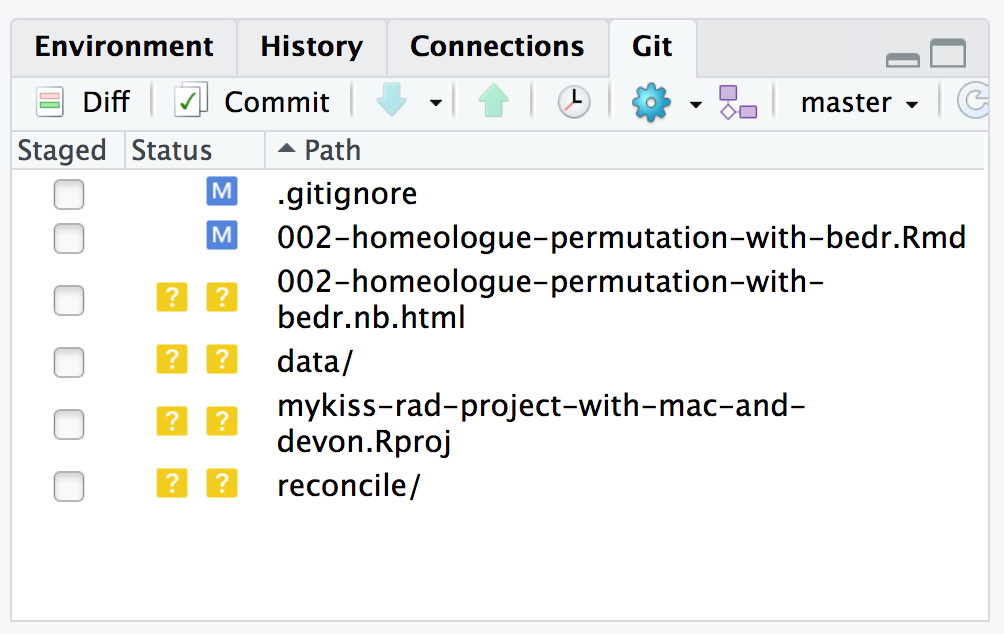
\includegraphics{figs/git-window} 

}

\caption{An example of what an RStudio git window might look like.}\label{fig:git-window}
\end{figure}

That view is merely showing you a graphical view of the output of
the \texttt{git\ status} command run at the top level of the repository which
looks like this:

\begin{Shaded}
\begin{Highlighting}[]
\ExtensionTok{%}\NormalTok{ git status}
\ExtensionTok{On}\NormalTok{ branch master}
\ExtensionTok{Changes}\NormalTok{ not staged for commit:}
  \KeywordTok{(}\ExtensionTok{use} \StringTok{"git add <file>..."}\NormalTok{ to update what will be committed}\KeywordTok{)}
  \KeywordTok{(}\ExtensionTok{use} \StringTok{"git checkout -- <file>..."}\NormalTok{ to discard changes in working directory}\KeywordTok{)}

    \ExtensionTok{modified}\NormalTok{:   .gitignore}
    \ExtensionTok{modified}\NormalTok{:   002-homeologue-permutation-with-bedr.Rmd}

\ExtensionTok{Untracked}\NormalTok{ files:}
  \KeywordTok{(}\ExtensionTok{use} \StringTok{"git add <file>..."}\NormalTok{ to include in what will be committed}\KeywordTok{)}

    \ExtensionTok{002-homeologue-permutation-with-bedr.nb.html}
    \ExtensionTok{data/}
    \ExtensionTok{mykiss-rad-project-with-mac-and-devon.Rproj}
    \ExtensionTok{reconcile/}

\ExtensionTok{no}\NormalTok{ changes added to commit (use }\StringTok{"git add"}\NormalTok{ and/or }\StringTok{"git commit -a"}\NormalTok{)}
\end{Highlighting}
\end{Shaded}

Aha! Be sure to read that and understand that the output tells you which
files are tracked by git and Modified (blue M in RStudio) and which
are untracked (Yellow ? in RStudio).

Of you wanted to see a report of the changes in the files relative
to the currently committed version, you could use \texttt{git\ diff}, passing
it the file name as an argument. We will see an example of that below\ldots{}

Now, recall, that in order to commit files to \texttt{git} you first must
\emph{stage} them. In RStudio you do that by clicking the little button to
the left of the file or directory in the Git window. For example,
if we clicked the buttons for the \texttt{data/} directory, as well as for
\texttt{.gitignore} and \texttt{002-homeologue-permutation-with-bedr.Rmd}, we would
have staged them and it would look like Figure \ref{fig:git-staged}.

\begin{figure}

{\centering 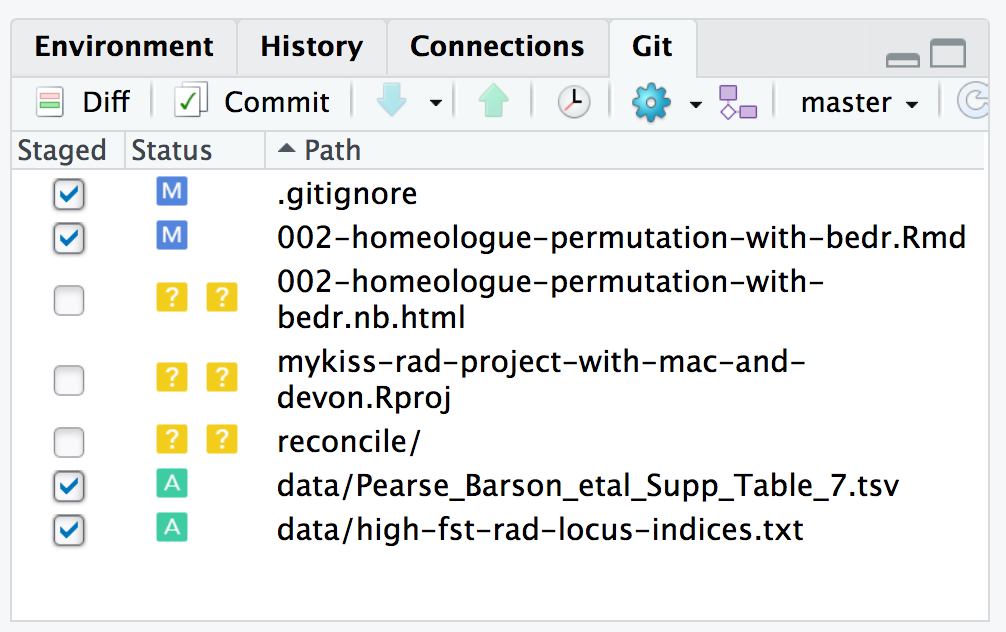
\includegraphics{figs/git-staged} 

}

\caption{An example of what an RStudio git window might look like.}\label{fig:git-staged}
\end{figure}

In order to do the equivalent operations with \texttt{git} on the command line
you would use the \texttt{git\ add} command, explicitly naming the files you wish to
\emph{stage} for committing:

\begin{Shaded}
\begin{Highlighting}[]
\FunctionTok{git}\NormalTok{ add .gitignore 002-homeologue-permutation-with-bedr.Rmd data}
\end{Highlighting}
\end{Shaded}

Now, if you check \texttt{git\ status} you will see:

\begin{Shaded}
\begin{Highlighting}[]
\ExtensionTok{%}\NormalTok{ git status}
\ExtensionTok{On}\NormalTok{ branch master}
\ExtensionTok{Changes}\NormalTok{ to be committed:}
  \KeywordTok{(}\ExtensionTok{use} \StringTok{"git reset HEAD <file>..."}\NormalTok{ to unstage}\KeywordTok{)}

    \ExtensionTok{modified}\NormalTok{:   .gitignore}
    \ExtensionTok{modified}\NormalTok{:   002-homeologue-permutation-with-bedr.Rmd}
    \ExtensionTok{new}\NormalTok{ file:   data/Pearse_Barson_etal_Supp_Table_7.tsv}
    \ExtensionTok{new}\NormalTok{ file:   data/high-fst-rad-locus-indices.txt}

\ExtensionTok{Untracked}\NormalTok{ files:}
  \KeywordTok{(}\ExtensionTok{use} \StringTok{"git add <file>..."}\NormalTok{ to include in what will be committed}\KeywordTok{)}

    \ExtensionTok{002-homeologue-permutation-with-bedr.nb.html}
    \ExtensionTok{mykiss-rad-project-with-mac-and-devon.Rproj}
    \ExtensionTok{reconcile/}
\end{Highlighting}
\end{Shaded}

It tells you which files are ready to be committed!

In order to commit the files to git you do:

\begin{Shaded}
\begin{Highlighting}[]
\FunctionTok{git}\NormalTok{ commit}
\end{Highlighting}
\end{Shaded}

And then, to push them back to GitHub (if you cloned this repository
from GitHub), you can simply do:

\begin{Shaded}
\begin{Highlighting}[]
\FunctionTok{git}\NormalTok{ push origin master}
\end{Highlighting}
\end{Shaded}

That syntax is telling git to push the \texttt{master} branch (which is
the default branch in a git repository), to the repository labeled as
\texttt{origin}, which will be the GitHub repository if you cloned the repository
from GitHub. (If you are working with a different git branch than master,
you would need to specify its name here. That is not difficult, but is
beyond the scope of this chapter.)

Now, assuming that we cloned the \texttt{alignment-play} repository to our
server, here are the steps involved in editing a file, committing the
changes, and then pushing them back to GitHub. The command in the following
is written as \texttt{{[}alignment-play{]}-\/-\%} which is telling us that we are in the
\texttt{alignment-play} repository.

\begin{Shaded}
\begin{Highlighting}[]
\CommentTok{# check git status}
\NormalTok{[}\ExtensionTok{alignment-play}\NormalTok{]--% git status}

\CommentTok{# On branch master}
\ExtensionTok{nothing}\NormalTok{ to commit, working directory clean}

\CommentTok{# Aha! That says nothing has been modified.}
\CommentTok{# But, now we edit the file alignment-play.Rmd}
\NormalTok{[}\ExtensionTok{alignment-play}\NormalTok{]--% nano alignment-play.Rmd}

\CommentTok{# In this case I merely added a line to the YAML header.}

\CommentTok{# Now, check status of the files:}
\NormalTok{[}\ExtensionTok{alignment-play}\NormalTok{]--% git status}

\CommentTok{# On branch master}
\CommentTok{# Changes not staged for commit:}
\CommentTok{#   (use "git add <file>..." to update what will be committed)}
\CommentTok{#   (use "git checkout -- <file>..." to discard changes in working directory)}
\CommentTok{#}
\CommentTok{#   modified:   alignment-play.Rmd}
\CommentTok{#}
\ExtensionTok{no}\NormalTok{ changes added to commit (use }\StringTok{"git add"}\NormalTok{ and/or }\StringTok{"git commit -a"}\NormalTok{)}

\CommentTok{# We see that the file has been modified.}

\CommentTok{# Now we can use git diff to see what the changes were}
\NormalTok{[}\ExtensionTok{alignment-play}\NormalTok{]--% git diff alignment-play.Rmd }

\FunctionTok{diff}\NormalTok{ --git a/alignment-play.Rmd b/alignment-play.Rmd}
\ExtensionTok{index}\NormalTok{ 9f75ebb..b389fae 100644}
\ExtensionTok{---}\NormalTok{ a/alignment-play.Rmd}
\ExtensionTok{+++}\NormalTok{ b/alignment-play.Rmd}
\ExtensionTok{@@}\NormalTok{ -3,6 +3,7 @@ title: }\StringTok{"Alignment Play!"}
 \ExtensionTok{output}\NormalTok{: }
   \ExtensionTok{html_notebook}\NormalTok{:}
     \ExtensionTok{toc}\NormalTok{: true}
\ExtensionTok{+}\NormalTok{    toc_float: true}
 \ExtensionTok{---}
 
\CommentTok{# The output above is a little hard to parse, but it shows}
\CommentTok{# the line that has been added: "  toc_float: true" with a}
\CommentTok{# "+" sign.}

\CommentTok{# In order to commit the changes, we do:}
\NormalTok{[}\ExtensionTok{alignment-play}\NormalTok{]--% git add alignment-play.Rmd }
\NormalTok{[}\ExtensionTok{alignment-play}\NormalTok{]--% git commit}

\CommentTok{# after that, we are bumped into the nano text editor}
\CommentTok{# to write a short message about the commit. After exiting}
\CommentTok{# from the editor, it tells us:}
\NormalTok{[}\ExtensionTok{master}\NormalTok{ 001e650] yaml change}
 \ExtensionTok{1}\NormalTok{ file changed, 1 insertion(+)}
 
\CommentTok{# Now, to send that new commit to GitHub, we use git push origin master}
\NormalTok{[}\ExtensionTok{alignment-play}\NormalTok{]--% git push origin master}
\ExtensionTok{Password}\NormalTok{ for }\StringTok{'https://eriqande@github.com'}\NormalTok{:}

\ExtensionTok{Counting}\NormalTok{ objects: 5, done.}
\ExtensionTok{Delta}\NormalTok{ compression using up to 24 threads.}
\ExtensionTok{Compressing}\NormalTok{ objects: 100% (3/3), }\KeywordTok{done}\ExtensionTok{.}
\ExtensionTok{Writing}\NormalTok{ objects: 100% (3/3), }\ExtensionTok{325}\NormalTok{ bytes }\KeywordTok{|} \ExtensionTok{0}\NormalTok{ bytes/s, done.}
\ExtensionTok{Total}\NormalTok{ 3 (delta 2), }\ExtensionTok{reused}\NormalTok{ 0 (delta 0)}
\ExtensionTok{remote}\NormalTok{: Resolving deltas: 100% (2/2), }\ExtensionTok{completed}\NormalTok{ with 2 local objects.}
\ExtensionTok{To}\NormalTok{ https://eriqande@github.com/eriqande/alignment-play}
   \ExtensionTok{0c1707f..001e650}\NormalTok{  master -}\OperatorTok{>}\NormalTok{ master}
\end{Highlighting}
\end{Shaded}

When pushing to a GitHub repository for the first
time from your remote server you
will be asked for your GitHub password. Once you have successfully
provided your password, if you set password caching up correctly, then
you should not have to provide your password for subsequent pushes.

Finally, if after pushing those changes to GitHub, we then pull them
down to our laptop, and make more changes on top of them and push those
back to GitHub, we can retrieve from GitHub to the server those changes we
made on our laptop with \texttt{git\ pull\ origin\ master}. In other words, from the
server we simply issue the command:

\begin{Shaded}
\begin{Highlighting}[]
\NormalTok{[}\ExtensionTok{alignment-play}\NormalTok{]--% git pull origin master}
\end{Highlighting}
\end{Shaded}

\hypertarget{globus}{%
\subsection{Globus}\label{globus}}

\hypertarget{interfacing-with-the-cloud}{%
\subsection{Interfacing with ``The Cloud''}\label{interfacing-with-the-cloud}}

Increasingly, data scientists and tech companies alike are keeping their
data ``in the cloud.'' This means that they
pay a large tech firm like Amazon, Dropbox, or Google to store their data for them in
a place that can be accessed via the internet. There are many advantages to this
model. For one thing, the company that serves the data often will create multiple copies
of the data for backup and redundancy: a fire in a single data center is not a calamity
because the data are also stored elsewhere, and can often be accessed seamlessly from those
other locations with no apparent disruption of service. For another, companies that are
in the business of storing and serving
data to multiple clients have data centers that are well-networked, so that getting
data onto and off of their storage systems can be done very quickly over the internet
by an end-user with a good internet connection.

Five years ago, the idea of storing next generation sequencing data might have
sounded a little
crazy---it always seemed a laborious task getting the data off of the remote server at the
sequencing center, so why not just keep the data in-house once you have it?
To be sure, keeping a copy of your
data in-house still can make sense for long-term data archiving needs, but, today, cloud
storage for your sequencing data can make a lot of sense. A few reasons are:

\begin{enumerate}
\def\labelenumi{\arabic{enumi}.}
\tightlist
\item
  Transferring your data from the cloud to the remote HPC system
  that you use to process the data can be very fast.
\item
  As above, your data can be redundantly backed up.
\item
  If your institution (university, agency, etc.) has an agreement with a cloud storage
  service that provides you with unlimited storage and free network access, then storing
  your sequencing data in the cloud will cost considerably less than buying a dedicated
  large system of hard drives for data backup. (One must wonder if service
  agreements might not be at risk of renegotiation if many researchers start using their
  unlimited institutional cloud storage space to store and/or archive their
  next generation sequencing data sets. My own agency's contract with Google runs
  through 2021\ldots{}but I have to think that these services are making plenty of money, even
  if a handful of researchers store big sequence data in the cloud. Nonetheless, you
  should be careful not to put multiple copies of data sets, or intermediate files that
  are easily regenerated, up in the cloud.)
\item
  If you are a PI with many lab members wishing to access the same data set, or even if
  you are just a regular Joe/Joanna researcher but you wish to share your data, it is
  possible to effect that using your cloud service's sharing settings. We will discuss
  how to do this with Google Drive.
\end{enumerate}

There are clearly advantages to using the cloud, but one small hurdle remains. Most
of the time, working in an HPC environment, we are using Unix, which provides a consistent
set of tools for interfacing with other computers using SSH-based protocols (like \texttt{scp}
for copying files from one remote computer to another). Unfortunately, many common
cloud storage services do not offer an SSH based interface. Rather, they typically process
requests from clients using an HTTPS protocol. This protocol, which effectively runs the
world-wide web, is a natural choice for cloud services that most people will access
using a web browser; however, Unix does not traditionally come with a utility or command
to easily process the types of HTTPS transactions needed to network with
cloud storage. Furthermore, there must be some security when it comes to accessing
your cloud-based storage---you don't want everyone to be able to access your files, so
your cloud service needs to have some way of authenticating people
(you and your labmates for example) that are authorized to access your data.

These problems have been overcome by a utility called \texttt{rclone}, the product of a
comprehensive open-source software project that brings the functionality of the
\texttt{rsync} utility (a common Unix tool used to synchronize and mirror file systems)
to cloud-based storage. (Note: \texttt{rclone} has nothing to do with the R programming
language, despite its name that looks like an R package.)
Currently \texttt{rclone} provides a consistent interface for accessing
files from over 35 different cloud storage providers, including Box, Dropbox, Google Drive,
and Microsoft OneDrive. Binaries for \texttt{rclone} can be downloaded for your desktop
machine from \url{https://rclone.org/downloads/}. We will
talk about how to install it on your HPC system later.

Once \texttt{rclone} is installed and in your \texttt{PATH}, you invoke it in your terminal
with the command \texttt{rclone}. Before we get into the details of the various \texttt{rclone} subcommands,
it will be helpful to take a glance at the information \texttt{rclone} records when it
configures itself to talk to your cloud service. To do so, it creates a file called \texttt{\textasciitilde{}/.config/rclone/rclone.conf}, where it stores information about all the different
connections to cloud services you have set up. For example, that
file on my system looks like this:

\begin{verbatim}
[gdrive-rclone]
type = drive
scope = drive
root_folder_id = 1I2EDV465N5732Tx1FFAiLWOqZRJcAzUd
token = {"access_token":"bs43.94cUFOe6SjjkofZ","token_type":"Bearer","refresh_token":"1/MrtfsRoXhgc","expiry":"2019-04-29T22:51:58.148286-06:00"}
client_id = 2934793-oldk97lhld88dlkh301hd.apps.googleusercontent.com
client_secret = MMq3jdsjdjgKTGH4rNV_y-NbbG
\end{verbatim}

In this configuration:

\begin{itemize}
\tightlist
\item
  \texttt{gdrive-rclone} is the name by which rclone refers to this cloud storage location
\item
  \texttt{root\_folder\_id} is the ID of the Google Drive folder that can be thought of as the root directory of \texttt{gdrive-rclone}. This ID is not the simple name of that directory on
  your Google Drive, rather it is the unique name given by Google Drive to that directory.
  You can see it by navigating in your browser to the directory you want and finding it
  after the last slash in the URL. For example, in the above case, the URL is:
  \texttt{https://drive.google.com/drive/u/1/folders/1I2EDV465N5732Tx1FFAiLWOqZRJcAzUd}
\item
  \texttt{client\_id} and \texttt{client\_secret} are like a username and a shared secret that \texttt{rclone} uses
  to authenticate the user to Google Drive as who they say they are.
\item
  \texttt{token} are the credentials used by \texttt{rclone} to make requests of Google Drive on the basis
  of the user.
\end{itemize}

Note: the above does not include my
real credentials, as then anyone could use them to access my Google Drive!

To set up your own configuration file to use Google Drive, you will use the \texttt{rclone\ config}
command, but before you do that, you will want to wrangle a client\_id from Google. Follow
the directions at \url{https://rclone.org/drive/\#making-your-own-client-id}. Things are a little different from in their step
by step, but you can muddle through to get to a screen with a client\_ID and a client
secret that you can copy onto your clipboard.

Once you have done that, then run \texttt{rclone\ config} and follow the prompts. A
typical session of \texttt{rclone\ config} for Google Drive access is given
\href{https://rclone.org/drive/}{here}. Don't choose to do the advanced setup; however
do use ``auto config,'' which will bounce up a web page and let you authenticate rclone
to your Google account.

It is worthwhile first setting up a config file on your laptop, and making sure
that it is working. After that, you can copy that config file to other remote
servers you work on and immediately have the same functionality.

\hypertarget{encrypting-your-config-file}{%
\subsubsection{Encrypting your config file}\label{encrypting-your-config-file}}

While it is a powerful thing to be able to copy a config file from
one computer to the next and immediately be able to access your Google
Drive account. That might (and should) also make you a little bit
uneasy. It means that if the config file falls into the wrong hands,
whoever has it can gain access to everything on your Google Drive. Clearly
this is not good. Consequently, once you have created your rclone config
file, and well before you transfer it to another computer, you must
encrypt it. This makes sense, and fortunately it is fairly easy: you can
use \texttt{rclone\ config} and see that encryption is one of
the options. When it is encrypted, use \texttt{rclone\ config\ show} to see what
it looks like in clear text.

The downside of using encryption is that you have to enter your password
every time you make an rclone command, but it is worth it to have the
security.

Here is what it looks like when choosing to encrypt one's config file:

\begin{Shaded}
\begin{Highlighting}[]
\ExtensionTok{%}\NormalTok{ rclone config}
\ExtensionTok{Current}\NormalTok{ remotes:}

\ExtensionTok{Name}\NormalTok{                 Type}
\NormalTok{====                 ====}
\ExtensionTok{gdrive-rclone}\NormalTok{        drive}

\ExtensionTok{e}\NormalTok{) }\ExtensionTok{Edit}\NormalTok{ existing remote}
\ExtensionTok{n}\NormalTok{) }\ExtensionTok{New}\NormalTok{ remote}
\ExtensionTok{d}\NormalTok{) }\ExtensionTok{Delete}\NormalTok{ remote}
\ExtensionTok{r}\NormalTok{) }\ExtensionTok{Rename}\NormalTok{ remote}
\ExtensionTok{c}\NormalTok{) }\ExtensionTok{Copy}\NormalTok{ remote}
\ExtensionTok{s}\NormalTok{) }\ExtensionTok{Set}\NormalTok{ configuration password}
\ExtensionTok{q}\NormalTok{) }\ExtensionTok{Quit}\NormalTok{ config}
\ExtensionTok{e/n/d/r/c/s}\NormalTok{/}\ExtensionTok{q}\OperatorTok{>}\NormalTok{ s }
\ExtensionTok{Your}\NormalTok{ configuration is not encrypted.}
\ExtensionTok{If}\NormalTok{ you add a password, you will protect your login information to cloud services.}
\ExtensionTok{a}\NormalTok{) }\ExtensionTok{Add}\NormalTok{ Password}
\ExtensionTok{q}\NormalTok{) }\ExtensionTok{Quit}\NormalTok{ to main menu}
\ExtensionTok{a}\NormalTok{/}\ExtensionTok{q}\OperatorTok{>}\NormalTok{ a}
\ExtensionTok{Enter}\NormalTok{ NEW configuration password:}
\ExtensionTok{password}\NormalTok{:}
\ExtensionTok{Confirm}\NormalTok{ NEW configuration password:}
\ExtensionTok{password}\NormalTok{:}
\ExtensionTok{Password}\NormalTok{ set}
\ExtensionTok{Your}\NormalTok{ configuration is encrypted.}
\ExtensionTok{c}\NormalTok{) }\ExtensionTok{Change}\NormalTok{ Password}
\ExtensionTok{u}\NormalTok{) }\ExtensionTok{Unencrypt}\NormalTok{ configuration}
\ExtensionTok{q}\NormalTok{) }\ExtensionTok{Quit}\NormalTok{ to main menu}
\ExtensionTok{c/u}\NormalTok{/}\ExtensionTok{q}\OperatorTok{>}\NormalTok{ q}
\ExtensionTok{Current}\NormalTok{ remotes:}

\ExtensionTok{Name}\NormalTok{                 Type}
\NormalTok{====                 ====}
\ExtensionTok{gdrive-rclone}\NormalTok{        drive}

\ExtensionTok{e}\NormalTok{) }\ExtensionTok{Edit}\NormalTok{ existing remote}
\ExtensionTok{n}\NormalTok{) }\ExtensionTok{New}\NormalTok{ remote}
\ExtensionTok{d}\NormalTok{) }\ExtensionTok{Delete}\NormalTok{ remote}
\ExtensionTok{r}\NormalTok{) }\ExtensionTok{Rename}\NormalTok{ remote}
\ExtensionTok{c}\NormalTok{) }\ExtensionTok{Copy}\NormalTok{ remote}
\ExtensionTok{s}\NormalTok{) }\ExtensionTok{Set}\NormalTok{ configuration password}
\ExtensionTok{q}\NormalTok{) }\ExtensionTok{Quit}\NormalTok{ config}
\ExtensionTok{e/n/d/r/c/s}\NormalTok{/}\ExtensionTok{q}\OperatorTok{>}\NormalTok{ q}
\end{Highlighting}
\end{Shaded}

Once that file is encrypted, you can copy it to other machines for use.

\hypertarget{basic-maneuvers}{%
\subsubsection{Basic Maneuvers}\label{basic-maneuvers}}

The syntax for use is:

\begin{Shaded}
\begin{Highlighting}[]
\ExtensionTok{rclone}\NormalTok{ [options] subcommand  parameter1 [parameter 2...]}
\end{Highlighting}
\end{Shaded}

The ``subcommand'' part tells \texttt{rclone} what you want to do, like \texttt{copy} or \texttt{sync}, and
the ``parameter'' part of the above syntax is typically a path
specification to a directory or a file. In using rclone to access the
cloud there is not a root directory, like \texttt{/} in Unix. Instead, each remote
cloud access point is treated as the root directory, and you refer to it
by the name of the configuration followed by a colon. In our example,
\texttt{gdrive-rclone:} is the root, and we don't need to add a \texttt{/} after it to
start a path with it. Thus \texttt{gdrive-rclone:this\_dir/that\_dir} is a
valid path for \texttt{rclone} to a location on my Google Drive.

Very often when moving, copying, or syncing files, the parameters
consist of:

\begin{Shaded}
\begin{Highlighting}[]
\NormalTok{source-directory  destination-directory}
\end{Highlighting}
\end{Shaded}

One very important point is that, unlike the Unix commands \texttt{cp} and \texttt{mv}, rclone
likes to operate on directories, not on multiple named files.

A few key subcommands:

\begin{itemize}
\tightlist
\item
  \texttt{ls}, \texttt{lsd}, and \texttt{lsl} are like \texttt{ls}, \texttt{ls\ -d} and \texttt{ls\ -l}
\end{itemize}

\begin{Shaded}
\begin{Highlighting}[]
\ExtensionTok{rclone}\NormalTok{  lsd gdrive-rclone:}
\ExtensionTok{rclone}\NormalTok{  lsd gdrive-rclone:NOFU}
\end{Highlighting}
\end{Shaded}

\begin{itemize}
\tightlist
\item
  \texttt{copy}: copy the \emph{contents} of a source \emph{directory} to a destination \emph{directory}. One super cool
  thing about this is that \texttt{rclone} won't re-copy files that are already on the destination and which
  are identical to those in the source directory.
\end{itemize}

\begin{Shaded}
\begin{Highlighting}[]
\ExtensionTok{rclone}\NormalTok{ copy bams gdrive-rclone:NOFU/bams}
\end{Highlighting}
\end{Shaded}

Note that the destination directory will be created if it does not already exist.\\
- \texttt{sync}: make the contents of the destination directory look just like the
contents of the source directory. \emph{WARNING} This will delete files in the destination
directory that do not appear in the source directory.

A few key options:

\begin{itemize}
\tightlist
\item
  \texttt{-\/-dry-run}: don't actually copy, sync, or move anything. Just tell me what you would have done.
\item
  \texttt{-\/-progress}: give me progress information when files are being copied.
  This will tell you which file is being transferred, the rate at which
  files are being transferred, and and estimated amount of time for all the
  files to be transferred.
\item
  \texttt{-\/-tpslimit\ 10}: don't make any more than 10 transactions a second with Google Drive (should always be used when transferring files)
\item
  \texttt{-\/-\/-fast-list}: combine multiple transactions together. Should always be used with Google Drive,
  especially when handling lots of files.
\item
  \texttt{-\/-drive-shared-with-me}: make the ``root'' directory a directory that shows all
  of the Google Drive folders that people have shared with you. This is key for accessing
  folders that have been shared with you.
\end{itemize}

For example, try something like:

\begin{Shaded}
\begin{Highlighting}[]
\ExtensionTok{rclone}\NormalTok{ --drive-shared-with-me lsd gdrive-rclone:}
\end{Highlighting}
\end{Shaded}

\textbf{Important Configuration Notes!!} Rather than always giving the \texttt{-\/-progress}
option on the command line, or always having to remember to use
\texttt{-\/-fast-list} and \texttt{-\/-tpslimit\ 10} (and remember what they should be\ldots{}),
you can set those options to be invoked ``by default'' whenever you use
rclone. The developers of \texttt{rclone} have made this possible
by setting \emph{environment variables} in your \texttt{\textasciitilde{}/.bashrc}.

If you have an rclone option called \texttt{-\/-fast-limit}, then the corresponding
environment variable is named \texttt{RCLONE\_FAST\_LIMIT}---basically, you
start with \texttt{RCLONE\_} then you just
drop the first two dashes of the option name, replace the remaining dashes
with underscores, and turn it all into uppercase to make the
environment variable. So, you should, at a minimum add these
lines to your \texttt{\textasciitilde{}/.bashrc}:

\begin{Shaded}
\begin{Highlighting}[]
\CommentTok{# Environment variables to use with rclone/google drive always}
\BuiltInTok{export} \VariableTok{RCLONE_TPSLIMIT=}\NormalTok{10}
\BuiltInTok{export} \VariableTok{RCLONE_FAST_LIST=}\NormalTok{true}
\BuiltInTok{export} \VariableTok{RCLONE_PROGRESS=}\NormalTok{true}
\end{Highlighting}
\end{Shaded}

\hypertarget{rclone-filter}{%
\subsubsection{filtering: Be particular about the files you transfer}\label{rclone-filter}}

\texttt{rclone} works a little differently than the Unix utility \texttt{cp}. In particular,
\texttt{rclone} is not set up very well to copy individual files. While there is a
an \texttt{rclone} command known as \texttt{copyto} that will allow you copy a single file,
you cannot (apparently) specify multiple, individual files that you wish to copy.

In other words, you can't do:

\begin{Shaded}
\begin{Highlighting}[]
\ExtensionTok{rclone}\NormalTok{ copyto this_file.txt that_file.txt another_file.bam gdrive-rclone:dest_dir}
\end{Highlighting}
\end{Shaded}

In general, you will be better off using \texttt{rclone} to copy the \emph{contents} of a directory
to the inside of the destination directory. However, there are options in \texttt{rclone} that
can keep you from being totally indiscriminate about the files you transfer. In other words,
you can \emph{filter} the files that get transferred. You can read about that at
\url{https://rclone.org/filtering/}.

For a quick example, imagine that you have a directory called \texttt{Data} on you Google Drive
that contains both VCF and BAM files. You want to get only the VCF files (ending with \texttt{.vcf.gz}, say)
onto the current working directory on your cluster. Then something like this works:

\begin{Shaded}
\begin{Highlighting}[]
\ExtensionTok{rclone}\NormalTok{ copy --include *.vcf.gz gdrive-rclone:Data ./}
\end{Highlighting}
\end{Shaded}

Note that, if you are issuing this command on a Unix system in a directory
where the pattern \texttt{*.vcf.gz} will expand (by globbing) to multiple files, you will
get an error. In that case, wrap the pattern in a pair of single quotes to keep
the shell from expanding it, like this:

\begin{Shaded}
\begin{Highlighting}[]
\ExtensionTok{rclone}\NormalTok{ copy --include }\StringTok{'*.vcf.gz'}\NormalTok{ gdrive-rclone:Data ./}
\end{Highlighting}
\end{Shaded}

\hypertarget{feel-free-to-make-lots-of-configurations}{%
\subsubsection{Feel free to make lots of configurations}\label{feel-free-to-make-lots-of-configurations}}

You might want to configure a remote for each directory-specific project.
You can do that by just editing the configuration file. For example,
if I had a directory deep within my Google Drive, inside a chain of folders that
looked like, say, \texttt{Projects/NGS/Species/Salmon/Chinook/CentralValley/WinterRun}
where I was keeping
all my data on a project concerning winter-run Chinook salmon, then it would be
quite inconvenient to type \texttt{Projects/NGS/Species/Salmon/Chinook/CentralValley/WinterRun}
every time I wanted to copy or sync something within that directory. Instead,
I could add the following
lines to my configuration file, essentially copying the existing configuration and
then modifying the configuration name and the \texttt{root\_folder\_id} to be the
Google Drive identifier for the folder \texttt{Projects/NGS/Species/Salmon/Chinook/CentralValley/WinterRun} (which
one can find by navigating to that folder in a web browser and pulling the ID from the
end of the URL.) The updated configuration could look like:

\begin{verbatim}
[gdrive-winter-run]
type = drive
scope = drive
root_folder_id = 1MjOrclmP1udhxOTvLWDHFBVET1dF6CIn
token = {"access_token":"bs43.94cUFOe6SjjkofZ","token_type":"Bearer","refresh_token":"1/MrtfsRoXhgc","expiry":"2019-04-29T22:51:58.148286-06:00"}
client_id = 2934793-oldk97lhld88dlkh301hd.apps.googleusercontent.com
client_secret = MMq3jdsjdjgKTGH4rNV_y-NbbG
\end{verbatim}

As long as the directory is still within the same Google Drive account, you can re-use
all the authorization information, and just change the \texttt{{[}name{]}} part and the \texttt{root\_folder\_id}.
Now this:

\begin{Shaded}
\begin{Highlighting}[]
\ExtensionTok{rclone}\NormalTok{ copy src_dir gdrive-winter-run: }
\end{Highlighting}
\end{Shaded}

puts items into \texttt{Projects/NGS/Species/Salmon/Chinook/CentralValley/WinterRun} on the Google Drive
without having to type that God-awful long path name.

\hypertarget{installing-rclone-on-a-remote-machine-without-sudo-access}{%
\subsubsection{Installing rclone on a remote machine without sudo access}\label{installing-rclone-on-a-remote-machine-without-sudo-access}}

The instructions on the website require root access. You don't have to have root
access to install rclone locally in your home directory somewhere.
Copy the download link from \url{https://rclone.org/downloads/} for
the type of operating system your remote machine uses (most likely Linux if it is a cluster).
Then transfer that with \texttt{wget}, unzip it and put the binary in your PATH. It will look
something like this:

\begin{verbatim}
wget https://downloads.rclone.org/rclone-current-linux-amd64.zip
unzip rclone-current-linux-amd64.zip
cp rclone-current-linux-amd64/rclone ~/bin
\end{verbatim}

You won't get manual pages on your system, but you can always find the docs on the web.

\hypertarget{setting-up-configurations-on-the-remote-machine}{%
\subsubsection{Setting up configurations on the remote machine\ldots{}}\label{setting-up-configurations-on-the-remote-machine}}

Is as easy as copying your config file to where it should go, which
is easy to find using the command:

\begin{Shaded}
\begin{Highlighting}[]
\ExtensionTok{rclone}\NormalTok{ config file}
\end{Highlighting}
\end{Shaded}

\hypertarget{some-other-usage-tips}{%
\subsubsection{Some other usage tips}\label{some-other-usage-tips}}

Following an email exchange with Ren, I should mention how to do an md5
checksum on the remote server to make sure that everything is correctly there.

\hypertarget{get-seqs}{%
\subsection{Getting files from a sequencing center}\label{get-seqs}}

Very often sequencing centers will post all the data from a single
run of a machine at a secured (or unsecured) http address. You will
need to download those files to operate on them on your cluster or
local machine. However some of the files available on the server
will likely belong to other researchers and you don't want to waste time
downloading them.

Let's take an example. Suppose you are sent an email from the sequencing
center that says something like:

\begin{quote}
Your samples are AW\_F1 (female) and AW\_M1 (male).
You should be able to access the data from this link provided by YCGA:
\url{http://sysg1.cs.yale.edu:3010/5lnO9bs3zfa8LOhESfsYfq3Dc/061719/}
\end{quote}

You can easily access this web address using \texttt{rclone}. You could set up a new
remote in your rclone config to point to \texttt{http://sysg1.cs.yale.edu},
but, since you will only be using this once, to get your data, it makes
more sense to just specify the remote on the command line. This can be
done by passing \texttt{rclone} the URL address via the \texttt{-\/-http-url} option, and
then, after that, telling it what protocol to use by adding \texttt{:http:} to
the command. Here is what you would use to list the directories available
at the sequencing center URL:

\begin{Shaded}
\begin{Highlighting}[]
\CommentTok{# here is the command}
\ExtensionTok{%}\NormalTok{ rclone lsd --http-url http://sysg1.cs.yale.edu:3010/5lnO9bs3zfa8LOhESfsYfq3Dc/061719/ :http:}

\CommentTok{# and here is the output}
          \ExtensionTok{-1}\NormalTok{ 1969-12-31 16:00:00        -1 sjg73_fqs}
          \ExtensionTok{-1}\NormalTok{ 1969-12-31 16:00:00        -1 sjg73_supernova_fqs}
\end{Highlighting}
\end{Shaded}

Aha! There are two directories that might hold our sequencing data.
I wonder what is in those diretories? The \texttt{rclone\ tree} command is the
perfect way to drill down into those diretories and look at their contents:

\begin{Shaded}
\begin{Highlighting}[]
\ExtensionTok{%}\NormalTok{ rclone tree --http-url http://sysg1.cs.yale.edu:3010/5lnO9bs3zfa8LOhESfsYfq3Dc/061719/ :http:}
\ExtensionTok{/}
\NormalTok{├── }\ExtensionTok{sjg73_fqs}
\NormalTok{│   ├── }\ExtensionTok{AW_F1}
\NormalTok{│   │   ├── }\ExtensionTok{AW_F1_S2_L001_I1_001.fastq.gz}
\NormalTok{│   │   ├── }\ExtensionTok{AW_F1_S2_L001_R1_001.fastq.gz}
\NormalTok{│   │   └── }\ExtensionTok{AW_F1_S2_L001_R2_001.fastq.gz}
\NormalTok{│   ├── }\ExtensionTok{AW_M1}
\NormalTok{│   │   ├── }\ExtensionTok{AW_M1_S3_L001_I1_001.fastq.gz}
\NormalTok{│   │   ├── }\ExtensionTok{AW_M1_S3_L001_R1_001.fastq.gz}
\NormalTok{│   │   └── }\ExtensionTok{AW_M1_S3_L001_R2_001.fastq.gz}
\NormalTok{│   └── }\ExtensionTok{ESP_A1}
\NormalTok{│       ├── }\ExtensionTok{ESP_A1_S1_L001_I1_001.fastq.gz}
\NormalTok{│       ├── }\ExtensionTok{ESP_A1_S1_L001_R1_001.fastq.gz}
\NormalTok{│       └── }\ExtensionTok{ESP_A1_S1_L001_R2_001.fastq.gz}
\NormalTok{└── }\ExtensionTok{sjg73_supernova_fqs}
\NormalTok{    ├── }\ExtensionTok{AW_F1}
\NormalTok{    │   ├── }\ExtensionTok{AW_F1_S2_L001_I1_001.fastq.gz}
\NormalTok{    │   ├── }\ExtensionTok{AW_F1_S2_L001_R1_001.fastq.gz}
\NormalTok{    │   └── }\ExtensionTok{AW_F1_S2_L001_R2_001.fastq.gz}
\NormalTok{    ├── }\ExtensionTok{AW_M1}
\NormalTok{    │   ├── }\ExtensionTok{AW_M1_S3_L001_I1_001.fastq.gz}
\NormalTok{    │   ├── }\ExtensionTok{AW_M1_S3_L001_R1_001.fastq.gz}
\NormalTok{    │   └── }\ExtensionTok{AW_M1_S3_L001_R2_001.fastq.gz}
\NormalTok{    └── }\ExtensionTok{ESP_A1}
\NormalTok{        ├── }\ExtensionTok{ESP_A1_S1_L001_I1_001.fastq.gz}
\NormalTok{        ├── }\ExtensionTok{ESP_A1_S1_L001_R1_001.fastq.gz}
\NormalTok{        └── }\ExtensionTok{ESP_A1_S1_L001_R2_001.fastq.gz}

\ExtensionTok{8}\NormalTok{ directories, 18 files}
\end{Highlighting}
\end{Shaded}

Whoa! That is pretty cool!. From this output we see that there are
subdirectories named \texttt{AW\_F1} and \texttt{AW\_M1} that hold the files that
we want. And, of course, the \texttt{ESP\_A1} samples must belong to someone
else. It would be great if we could just download the files we wanted,
excluding the ones in the \texttt{ESP\_A1} directories. It turns out that there is!
\texttt{rclone} has an \texttt{-\/-exclude} option to exclude paths that match certain
patterns (see Section \ref{rclone-filter}, above). We can
experiment by giving \texttt{rclone\ copy} the \texttt{-\/-dry-run} command to see which
files will be transferred. If we don't do any filtering, we see this
when we try to dry-run copy the directories to our local directory \texttt{Alewife/fastqs}:

\begin{Shaded}
\begin{Highlighting}[]
\ExtensionTok{%}\NormalTok{ rclone copy --dry-run --http-url http://sysg1.cs.yale.edu:3010/5lnO9bs3zfa8LOhESfsYfq3Dc/061719/ :http: Alewife/fastqs/}
\ExtensionTok{2019/07/11}\NormalTok{ 10:33:43 NOTICE: sjg73_fqs/ESP_A1/ESP_A1_S1_L001_I1_001.fastq.gz: Not copying as --dry-run}
\ExtensionTok{2019/07/11}\NormalTok{ 10:33:43 NOTICE: sjg73_fqs/ESP_A1/ESP_A1_S1_L001_R1_001.fastq.gz: Not copying as --dry-run}
\ExtensionTok{2019/07/11}\NormalTok{ 10:33:43 NOTICE: sjg73_fqs/ESP_A1/ESP_A1_S1_L001_R2_001.fastq.gz: Not copying as --dry-run}
\ExtensionTok{2019/07/11}\NormalTok{ 10:33:43 NOTICE: sjg73_supernova_fqs/AW_M1/AW_M1_S3_L001_I1_001.fastq.gz: Not copying as --dry-run}
\ExtensionTok{2019/07/11}\NormalTok{ 10:33:43 NOTICE: sjg73_supernova_fqs/AW_M1/AW_M1_S3_L001_R1_001.fastq.gz: Not copying as --dry-run}
\ExtensionTok{2019/07/11}\NormalTok{ 10:33:43 NOTICE: sjg73_supernova_fqs/AW_M1/AW_M1_S3_L001_R2_001.fastq.gz: Not copying as --dry-run}
\ExtensionTok{2019/07/11}\NormalTok{ 10:33:43 NOTICE: sjg73_supernova_fqs/AW_F1/AW_F1_S2_L001_I1_001.fastq.gz: Not copying as --dry-run}
\ExtensionTok{2019/07/11}\NormalTok{ 10:33:43 NOTICE: sjg73_supernova_fqs/AW_F1/AW_F1_S2_L001_R1_001.fastq.gz: Not copying as --dry-run}
\ExtensionTok{2019/07/11}\NormalTok{ 10:33:43 NOTICE: sjg73_supernova_fqs/AW_F1/AW_F1_S2_L001_R2_001.fastq.gz: Not copying as --dry-run}
\ExtensionTok{2019/07/11}\NormalTok{ 10:33:43 NOTICE: sjg73_supernova_fqs/ESP_A1/ESP_A1_S1_L001_I1_001.fastq.gz: Not copying as --dry-run}
\ExtensionTok{2019/07/11}\NormalTok{ 10:33:43 NOTICE: sjg73_supernova_fqs/ESP_A1/ESP_A1_S1_L001_R1_001.fastq.gz: Not copying as --dry-run}
\ExtensionTok{2019/07/11}\NormalTok{ 10:33:43 NOTICE: sjg73_supernova_fqs/ESP_A1/ESP_A1_S1_L001_R2_001.fastq.gz: Not copying as --dry-run}
\ExtensionTok{2019/07/11}\NormalTok{ 10:33:43 NOTICE: sjg73_fqs/AW_F1/AW_F1_S2_L001_I1_001.fastq.gz: Not copying as --dry-run}
\ExtensionTok{2019/07/11}\NormalTok{ 10:33:43 NOTICE: sjg73_fqs/AW_F1/AW_F1_S2_L001_R1_001.fastq.gz: Not copying as --dry-run}
\ExtensionTok{2019/07/11}\NormalTok{ 10:33:43 NOTICE: sjg73_fqs/AW_F1/AW_F1_S2_L001_R2_001.fastq.gz: Not copying as --dry-run}
\ExtensionTok{2019/07/11}\NormalTok{ 10:33:43 NOTICE: sjg73_fqs/AW_M1/AW_M1_S3_L001_I1_001.fastq.gz: Not copying as --dry-run}
\ExtensionTok{2019/07/11}\NormalTok{ 10:33:43 NOTICE: sjg73_fqs/AW_M1/AW_M1_S3_L001_R1_001.fastq.gz: Not copying as --dry-run}
\ExtensionTok{2019/07/11}\NormalTok{ 10:33:43 NOTICE: sjg73_fqs/AW_M1/AW_M1_S3_L001_R2_001.fastq.gz: Not copying as --dry-run}
\end{Highlighting}
\end{Shaded}

Since we do not want to copy the \texttt{ESP\_A1} files we see if we can exclude
them:

\begin{Shaded}
\begin{Highlighting}[]
\ExtensionTok{%}\NormalTok{ rclone copy --exclude */ESP_A1/* --dry-run --http-url http://sysg1.cs.yale.edu:3010/5lnO9bs3zfa8LOhESfsYfq3Dc/061719/ :http: Alewife/fastqs/}
\ExtensionTok{2019/07/11}\NormalTok{ 10:37:22 NOTICE: sjg73_fqs/AW_F1/AW_F1_S2_L001_I1_001.fastq.gz: Not copying as --dry-run}
\ExtensionTok{2019/07/11}\NormalTok{ 10:37:22 NOTICE: sjg73_fqs/AW_F1/AW_F1_S2_L001_R2_001.fastq.gz: Not copying as --dry-run}
\ExtensionTok{2019/07/11}\NormalTok{ 10:37:22 NOTICE: sjg73_fqs/AW_F1/AW_F1_S2_L001_R1_001.fastq.gz: Not copying as --dry-run}
\ExtensionTok{2019/07/11}\NormalTok{ 10:37:22 NOTICE: sjg73_fqs/AW_M1/AW_M1_S3_L001_I1_001.fastq.gz: Not copying as --dry-run}
\ExtensionTok{2019/07/11}\NormalTok{ 10:37:22 NOTICE: sjg73_fqs/AW_M1/AW_M1_S3_L001_R2_001.fastq.gz: Not copying as --dry-run}
\ExtensionTok{2019/07/11}\NormalTok{ 10:37:22 NOTICE: sjg73_fqs/AW_M1/AW_M1_S3_L001_R1_001.fastq.gz: Not copying as --dry-run}
\ExtensionTok{2019/07/11}\NormalTok{ 10:37:22 NOTICE: sjg73_supernova_fqs/AW_F1/AW_F1_S2_L001_I1_001.fastq.gz: Not copying as --dry-run}
\ExtensionTok{2019/07/11}\NormalTok{ 10:37:22 NOTICE: sjg73_supernova_fqs/AW_F1/AW_F1_S2_L001_R2_001.fastq.gz: Not copying as --dry-run}
\ExtensionTok{2019/07/11}\NormalTok{ 10:37:22 NOTICE: sjg73_supernova_fqs/AW_F1/AW_F1_S2_L001_R1_001.fastq.gz: Not copying as --dry-run}
\ExtensionTok{2019/07/11}\NormalTok{ 10:37:22 NOTICE: sjg73_supernova_fqs/AW_M1/AW_M1_S3_L001_I1_001.fastq.gz: Not copying as --dry-run}
\ExtensionTok{2019/07/11}\NormalTok{ 10:37:22 NOTICE: sjg73_supernova_fqs/AW_M1/AW_M1_S3_L001_R1_001.fastq.gz: Not copying as --dry-run}
\ExtensionTok{2019/07/11}\NormalTok{ 10:37:22 NOTICE: sjg73_supernova_fqs/AW_M1/AW_M1_S3_L001_R2_001.fastq.gz: Not copying as --dry-run}
\end{Highlighting}
\end{Shaded}

Booyah! That gets us just what we want. So, then we remove the \texttt{-\/-dry-run} option,
and maybe add \texttt{-v\ -P} to give us verbose output and progress information, and copy all of our files:

\begin{Shaded}
\begin{Highlighting}[]
\ExtensionTok{%}\NormalTok{ rclone copy --exclude */ESP_A1/* -v -P  --http-url http://sysg1.cs.yale.edu:3010/5lnO9bs3zfa8LOhESfsYfq3Dc/061719/ :http: Alewife/fastqs/}
\end{Highlighting}
\end{Shaded}

\hypertarget{tmux}{%
\section{\texorpdfstring{\texttt{tmux}: the terminal multiplexer}{tmux: the terminal multiplexer}}\label{tmux}}

Many universities have recently implemented a two-factor
authentication requirement for access to their computing resources
(like remote servers and clusters). This means that every time
you login to a server on campus (using \texttt{ssh} for example) you must
type your password, and also fiddle with your phone. Such systems
preclude the use of public/private key pairs that historically allowed
you to access a server from a trusted client (i.e., your own secured
laptop) without having to type in a password. As a consequence, today,
opening multiple sessions on a server using \texttt{ssh} and two-factor
authentication requires a ridiculous amount of additional typing and
phone-fiddling, and is a huge hassle. But, when working on a remote
server it is often very convenient to have multiple separate shells that
you are working on and can quickly switch between.

At the same time. When you are working on the shell of a remote machine
and your network connection goes down, then, typically the bash session on
your remote machine will be forcibly quit, killing any jobs that you might
have been in the middle of (however, this is not the case of you submitted
those jobs through a job scheduler like SLURM. Much more on that in the
next chapter.). And, finally, in a traditional
\texttt{ssh} session to a remote machine, when you close your laptop, or put it
to sleep, or quit the Terminal application, all of your active bash sessions
on the remote machine will get shut down. Consequently, the next time
you want to work on that project, after you have logged
onto that remote machine you will have to go through the laborious steps
of navigating to your desired working directory, starting up any processes
that might have gotten killed, and generally getting yourself
set up to work again. That is a serious buzz kill!

Fortunately, there is an awesome utility called \texttt{tmux}, which is short for
``terminal multiplexer'' that solves most of the problems we just described.
\texttt{tmux} is similar in function to a utility called \texttt{screen}, but it is easier
to use while at the same time being more customizable and configurable
(in my opinion). \texttt{tmux} is basically your ticket to working \emph{way} more
efficiently on remote computers, while at the same time looking
(to friends and colleagues, at least) like
the full-on, bad-ass Unix user.

In full confession, I didn't actually start using \texttt{tmux} until some
five years after a speaker at a workshop delivered an incredibly
enthusiastic presentation about \texttt{tmux} and how much he was in love
with it. In somewhat the same fashion that I didn't adopt RStudio shortly
after its release, because I had my own R workflows that I had hacked
together myself, I thought to myself: ``I have public/private key pairs
so it is super easy for me to just start another terminal window and login
to the server for a new session. Why would I need \texttt{tmux}?'' I also didn't
quite understand how \texttt{tmux} worked initially: I thought that I had to
run \texttt{tmux} simultaneously on my laptop and on the server, and that those
two processes would talk to one another. That is not the case! You
just have to run \texttt{tmux} on the server and all will work fine!
The upshot of that confession is that you should \emph{not} be a bozo like me,
and you should learn to use \texttt{tmux} \emph{right now}! You will thank yourself
for it many times over down the road.

\hypertarget{an-analogy-for-how-tmux-works}{%
\subsection{\texorpdfstring{An analogy for how \texttt{tmux} works}{An analogy for how tmux works}}\label{an-analogy-for-how-tmux-works}}

Imagine that the first time you log in to your remote server
you also have the option of speaking on the phone to a super
efficient IT guy who has a desk in the server room.
This dude never takes a break, but sits at his desk
24/7. He probably has mustard stains on his dingy white T-shirt
from eating ham sandwiches non-stop while he works super hard. This guy is Tmux.

When you \emph{first} speak to this guy after logging in, you have to preface your
commands with \texttt{tmux} (as in, ``Hey Tmux!''). He is there to help you
manage different terminal windows with different bash shells or
processes going on in them. In fact, you can think of it this way: you can
ask him to set up
a terminal (i.e., like a monitor), right there on his desk, and then create
a bunch of windows on that terminal for you---each
one with its own bash shell---without having to do a separate login for
each one. He has created all those windows, but you still get to use them.
It is like he has a miracle-mirroring device that lets you operate
the windows that are on the terminal he set up for you on his desk.

When you are done working on all those windows, you can tell Tmux that you
want to \emph{detach} from the special terminal he set up for you at the server.
In response he says, ``Cool!'' and shuts down his miracle-mirroring device, so
you no longer see those different windows. However, he \emph{does not} shut down the
terminal on his desk that he set up for you. That terminal stays on, and any of your processes
happening on it keep chugging away\ldots{}even after you logout from the server entirely,
throw the lid down on your laptop,
have drinks with your friends at Social, downtown, watch an episode
of Parks and Rec, and then get a good night's sleep.

All through the night, Tmux is munching ham sandwiches and keeping an eye on that
terminal he set up for you. When you log back onto the server in the morning, you
can say ``Hey Tmux! I want to attach back to that terminal you set up for me.'' He
says, ``No problem!'', turns his miracle-mirroring device back on, and in an instant
you have all of the windows on that terminal back on your laptop with all the processes
still running in them---in all the same working directories---just as you left it all
(except that if you were running jobs in those windows, some of those jobs might already
be done!).

Not only that, but, further, if you are working on the server when a local thunderstorm
fries the motherboard on your laptop, you can get a new laptop, log back into the
server and ask Tmux to reconnect you to that terminal and get back to all of those
windows and jobs, etc. as if you didn't get zapped. The same goes for the case of
a backhoe operator accidentally digging up the fiber optic cable in your yard. Your
network connection can go down completely. But, when you get it up and running again,
you can say ``Hey Tmux! Hook me up!'' and he'll say, ``No problem!'' and reconnect you
to all those windows you had open on the server.

Finally, when you are done with all the windows and jobs on the terminal that Tmux set
up for you, you can ask him to kill it, and he will shut it down, unplug it, and, straight
out of \emph{Office Space}, chuck it out the window. But he will gladly install a new one
if you want to start another \emph{session} with him.

That dude is super helpful!

\hypertarget{first-steps-with-tmux}\NormalTok{ which tmux}
\end{Highlighting}
\end{Shaded}

This should return something like:

\begin{verbatim}
/usr/bin/tmux
\end{verbatim}

If, instead, you get a response like \texttt{tmux:\ Command\ not\ found.} then \texttt{tmux}
is apparently not installed
on your remote server, so you
will have to install it yourself, or beg your sysadmin to do so (we will cover
that in a later chapter). If you
are working on the Summit supercomptuer in Colorado or on Hummingbird at
UCSC, then \texttt{tmux} is installed already. (As of Feb 16, 2020, \texttt{tmux} was
not installed on the Sedna cluster at the NWFSC, but I will request that it
be installed.)

In the analogy, above, we talked about Tmux setting up a terminal
in the server room. In \texttt{tmux} parlance, such a ``terminal'' is called
a \emph{session}. In order to be able to tell Tmux that you want to reconnect
to a session, you
will \emph{always} want to name your sessions so you will request a new
session with this syntax:

\begin{Shaded}
\begin{Highlighting}[]
\ExtensionTok{%}\NormalTok{ tmux new -s froggies}
\end{Highlighting}
\end{Shaded}

You can think of the \texttt{-s} as being short for ``session.'' So it is basically a short
way of saying, ``Hey Tmux, give me a new session named \texttt{froggies}.''
That creates a new session called \texttt{froggies}, and you can imagine we've
named it that because we will use it for work on a frog genomics project.

The effect of this
is like Tmux firing up a new terminal in his server room, making a
window on it for you, starting a new bash shell in that window,
\emph{and then giving you control of this new terminal}.
In other words, it is sort of like he has opened a new shell window on a
terminal for you, and is letting you see and use it on your computer at the same time.

One very cool thing about this is that you just got a new bash shell
without having to login with your password and two-factor authentication again.
That much is cool in itself, but is only the beginning.

The new window that you get looks a little different. For one thing, it
has a section, one line tall, that is green (by default) on the bottom.
In our case, on the left side it gives the name of the session (in square
brackets) and then the name of the current \emph{window} within that session. On
the right side you see the \emph{hostname} (the name of the remote computer
you are working on) in quotes, followed by the date and time. The contents
in that green band will look something
like:

\begin{verbatim}
[froggies] 0:bash*                                               "login11" 20:02 15-Feb-20
\end{verbatim}

This little line of information is the sweet sauce that will let you
find your way around all the new windows that
\texttt{tmux} can spawn for you.\\
\BeginKnitrBlock{rmdcaution}
If you are working on a cluster, please pay special attention to the hostname.
(In the above case the hostname is \texttt{login11}). Many clusters have multiple \emph{login}
or \emph{head} nodes, as they are called. The next time you login to the cluster, you
might be assigned to a different login node which will have no idea about your
\texttt{tmux} sessions. If that were the case in this example I would have to use \texttt{slogin\ login11} and
authenticate again to get logged into \texttt{login11} to reconnect to my
\texttt{tmux} session, \texttt{froggies}. Or, if you were a CSU student and wanted to login specifically to
the \texttt{login11} node on Summit the next time you logged on you could do
\texttt{ssh\ username@colostate.edu@login11.rc.colorado.edu}. Note the specific \texttt{login11} in that
statement.
\EndKnitrBlock{rmdcaution}

Now, imagine that we want to use this \emph{window} in our \texttt{froggies} \emph{session}, to look at some
frog data we have. Accordingly, we might navigate to the directory where those data live
and look at the data with \texttt{head} and \texttt{less}, etc. That is all great, until we realize that
we also want to edit some scripts that we wrote for processing our froggy data. These scripts
might be in a directory far removed from the data directory we are currently in, and we don't really
want to keep navigating back and forth between those two directories within a single bash shell.
Clearly, we would like to have two windows that we could switch between: one for inspecting
our data, and the other for editing our scripts.

We are in luck! We can do this with \texttt{tmux}. However, now that we are safely working in a \emph{session}
that \texttt{tmux} started for us, we no longer have to shout ``Hey Tmux!'' Rather we can just ``ring a little
bell'' to get his attention. In the default \texttt{tmux} configuration, you do that by pressing
\texttt{\textless{}cntrl\textgreater{}-b} from anywhere within a \texttt{tmux} window. This is easy to remember because it is like
a ``b'' for the ``bell'' that we ring to get our faithful servant's attention. \texttt{\textless{}cntrl\textgreater{}-b} is known
as the ``prefix'' sequence that starts all requests to \texttt{tmux} from within a session.

The first thing that we are going to do is ask \texttt{tmux} to let us assign a more descriptive,
name---\texttt{data} to be specific---to the current window. We do this with

\begin{verbatim}
<cntrl>-b ,
\end{verbatim}

(That's right! It's a control-b and then a comma. \texttt{tmux} likes to get by on a minimum number
of keystrokes.) When you do that, the green band at the bottom of the window changes color
and tells you that you can rename the current window. We simply use our keyboard to
change the name to ``data''. That was super easy!

Now, to make a new window with a new bash shell that we can use for writing scripts
we do \texttt{\textless{}cntrl\textgreater{}-b\ c}. Try it! That gives you a new \emph{window} within the \texttt{froggies} session
and switches your focus to it. It is as if Tmux (in his mustard-stained shirt) has created
a new window on the \texttt{froggies} terminal, brought it to the front, and shared it with you.
The left side of the green \texttt{tmux} status bar at the bottom of the screen now says:

\begin{verbatim}
[froggies] 0:data- 1:bash*
\end{verbatim}

Holy Moly! This is telling you that the \texttt{froggies} session has two windows in it: the first
numbered 0 and named \texttt{data}, and the second numbered 1 and named \texttt{bash}. The \texttt{-} at the end
of \texttt{0:data-} is telling you that \texttt{data} is the window you were previously focused on, but that
now you are currently focused on the window with the \texttt{*} after its name: \texttt{1:bash*}.

So, the name \texttt{bash} is not as informative as it could be. Since we will be using this
new window for editing scripts, let's rename it to \texttt{edit}. You can do that with
\texttt{\textless{}cntrl\textgreater{}-b\ ,}. Do it!

OK! Now, if you have been paying attention, you probably realize that \texttt{tmux} has given us
two windows (with two different bash shells) in this session called \texttt{froggies}. Not only that
but it has associated a single-digit number with each window. If you are all about keyboard
shortcuts, then you probably have already imagined that \texttt{tmux} will let you switch between
these two windows with \texttt{\textless{}cntrl\textgreater{}-b} plus a digit (0 or 1 in this case). Play with that.
Do \texttt{\textless{}cntrl\textgreater{}-b\ 0} and \texttt{\textless{}cntrl\textgreater{}-b\ 1} and feel the power!

Now, for fun, imagine that we want to have another window and a bash shell for launching
jobs. Make a new window, name it \texttt{launch}, and then switch between those three windows.

Finally. When you are done with all that, you tell Tmux to detach from this session
by typing:

\begin{verbatim}
<cntrl>-b d
\end{verbatim}

(The \texttt{d} is for ``detach''). This should kick you back to the shell from which you
first shouted ``Hey Tmux!'' by issuing the \texttt{tmux\ a\ -t\ froggies} command. So, you
can't see the windows of your \texttt{froggies} session any longer, \emph{but do not despair}!
Those windows are still on the monitor Tmux set up for you, casting an eerie glow
on his mustard stained shirt.

If you want to get back in the driver's seat with all of those windows, you simply need to
tell Tmux that you want to be attached again via his miracle-mirroring device. Since we
are no longer in a \texttt{tmux} window, we don't use our \texttt{\textless{}cntrl-b\textgreater{}} bell to get Tmux's attention.
We have to shout:

\begin{Shaded}
\begin{Highlighting}[]
\ExtensionTok\NormalTok{ tmux a -t froggies}
\end{Highlighting}
\end{Shaded}

Of course, sometimes, when you log back onto the server, you won't remember the name
of the \texttt{tmux} session(s) you started. Use this command to list them all:

\begin{Shaded}
\begin{Highlighting}[]
\ExtensionTok\NormalTok{ tmux ls}
\ExtensionTok{birdies}\NormalTok{: 4 windows (created Sun Feb 16 07:23:30 2020) [}\ExtensionTok{203x59}\NormalTok{]}
\ExtensionTok{fishies}\NormalTok{: 2 windows (created Sun Feb 16 07:23:55 2020) [}\ExtensionTok{203x59}\NormalTok{]}
\ExtensionTok{froggies}\NormalTok{: 3 windows (created Sun Feb 16 07:22:36 2020) [}\ExtensionTok{203x59}\NormalTok{]}
\end{Highlighting}
\end{Shaded}

That is enough to remind you of which session you might wish to reattach to.

Finally, if you are all done with a \texttt{tmux} session, and you have detached from it,
then from your shell prompt (not within a \texttt{tmux} session) you can do, for example:

\begin{Shaded}
\begin{Highlighting}[]
\ExtensionTok{tmux}\NormalTok{ kill-session -t  birdies}
\end{Highlighting}
\end{Shaded}

to kill the session. There are other ways to kill sessions while you
are in them, but that is not so much needed.

Table \ref{tab:minimal-tmux} reviews the minimal set of
\texttt{tmux} commands just described. Though there is much more that
can be done with \texttt{tmux}, those commands will get you started.

\begin{longtable}[]{@{}lll@{}}
\caption{\label{tab:minimal-tmux} A bare bones set of commands for using \texttt{tmux} The first column says whether the command is given within a \texttt{tmux} session rather than at the shell outside of a \texttt{tmux} session}\tabularnewline
\toprule
\begin{minipage}[b]{0.18\columnwidth}\raggedright
Within tmux?\strut
\end{minipage} & \begin{minipage}[b]{0.36\columnwidth}\raggedright
Command\strut
\end{minipage} & \begin{minipage}[b]{0.38\columnwidth}\raggedright
Effect\strut
\end{minipage}\tabularnewline
\midrule
\endfirsthead
\toprule
\begin{minipage}[b]{0.18\columnwidth}\raggedright
Within tmux?\strut
\end{minipage} & \begin{minipage}[b]{0.36\columnwidth}\raggedright
Command\strut
\end{minipage} & \begin{minipage}[b]{0.38\columnwidth}\raggedright
Effect\strut
\end{minipage}\tabularnewline
\midrule
\endhead
\begin{minipage}[t]{0.18\columnwidth}\raggedright
N\strut
\end{minipage} & \begin{minipage}[t]{0.36\columnwidth}\raggedright
\texttt{tmux\ ls}\strut
\end{minipage} & \begin{minipage}[t]{0.38\columnwidth}\raggedright
List any tmux sessions the
server knows about\strut
\end{minipage}\tabularnewline
\begin{minipage}[t]{0.18\columnwidth}\raggedright
N\strut
\end{minipage} & \begin{minipage}[t]{0.36\columnwidth}\raggedright
\texttt{tmux\ new\ -s\ name}\strut
\end{minipage} & \begin{minipage}[t]{0.38\columnwidth}\raggedright
Create a new tmux session
named ``name''\strut
\end{minipage}\tabularnewline
\begin{minipage}[t]{0.18\columnwidth}\raggedright
N\strut
\end{minipage} & \begin{minipage}[t]{0.36\columnwidth}\raggedright
\texttt{tmux\ attach\ -t\ name}\strut
\end{minipage} & \begin{minipage}[t]{0.38\columnwidth}\raggedright
Attach to the existing tmux
session ``name''\strut
\end{minipage}\tabularnewline
\begin{minipage}[t]{0.18\columnwidth}\raggedright
N\strut
\end{minipage} & \begin{minipage}[t]{0.36\columnwidth}\raggedright
\texttt{tmux\ a\ -t\ name}\strut
\end{minipage} & \begin{minipage}[t]{0.38\columnwidth}\raggedright
Same as ``attach'' but shorter.\strut
\end{minipage}\tabularnewline
\begin{minipage}[t]{0.18\columnwidth}\raggedright
N\strut
\end{minipage} & \begin{minipage}[t]{0.36\columnwidth}\raggedright
\texttt{tmux\ kill-session\ -t} name\strut
\end{minipage} & \begin{minipage}[t]{0.38\columnwidth}\raggedright
Kill the tmux session named
``name''\strut
\end{minipage}\tabularnewline
\begin{minipage}[t]{0.18\columnwidth}\raggedright
Y\strut
\end{minipage} & \begin{minipage}[t]{0.36\columnwidth}\raggedright
\texttt{\textless{}cntrl\textgreater{}-b\ ,}\strut
\end{minipage} & \begin{minipage}[t]{0.38\columnwidth}\raggedright
Edit the name of the current
window\strut
\end{minipage}\tabularnewline
\begin{minipage}[t]{0.18\columnwidth}\raggedright
Y\strut
\end{minipage} & \begin{minipage}[t]{0.36\columnwidth}\raggedright
\texttt{\textless{}cntrl\textgreater{}-b\ c}\strut
\end{minipage} & \begin{minipage}[t]{0.38\columnwidth}\raggedright
Create a new window\strut
\end{minipage}\tabularnewline
\begin{minipage}[t]{0.18\columnwidth}\raggedright
Y\strut
\end{minipage} & \begin{minipage}[t]{0.36\columnwidth}\raggedright
\texttt{\textless{}cntrl\textgreater{}-b\ 3}\strut
\end{minipage} & \begin{minipage}[t]{0.38\columnwidth}\raggedright
Move focus to window 3\strut
\end{minipage}\tabularnewline
\begin{minipage}[t]{0.18\columnwidth}\raggedright
Y\strut
\end{minipage} & \begin{minipage}[t]{0.36\columnwidth}\raggedright
\texttt{\textless{}cntrl\textgreater{}-b\ \&}\strut
\end{minipage} & \begin{minipage}[t]{0.38\columnwidth}\raggedright
Kill current window\strut
\end{minipage}\tabularnewline
\begin{minipage}[t]{0.18\columnwidth}\raggedright
Y\strut
\end{minipage} & \begin{minipage}[t]{0.36\columnwidth}\raggedright
\texttt{\textless{}cntrl\textgreater{}-b\ d}\strut
\end{minipage} & \begin{minipage}[t]{0.38\columnwidth}\raggedright
Detach from current session\strut
\end{minipage}\tabularnewline
\begin{minipage}[t]{0.18\columnwidth}\raggedright
Y\strut
\end{minipage} & \begin{minipage}[t]{0.36\columnwidth}\raggedright
\texttt{\textless{}cntrl\textgreater{}-l}\strut
\end{minipage} & \begin{minipage}[t]{0.38\columnwidth}\raggedright
Clear screen current window\strut
\end{minipage}\tabularnewline
\bottomrule
\end{longtable}

\hypertarget{further-steps-with-tmux}{%
\subsection{\texorpdfstring{Further steps with \texttt{tmux}}{Further steps with tmux}}\label{further-steps-with-tmux}}

The previous section merely scratched the surface of what is possible with \texttt{tmux}.\\
Indeed, that is the case with this section. But here I just want to leave you with a
taste for how to configure \texttt{tmux} to your liking, and also with the ability to create
different \emph{panes} within a window within a session. You guessed it! A pane is made by
splitting a \emph{window} (which is itself a part of a \emph{session}) into two different
sections, each one running its own bash shell.

Before we start making panes, we set some configurations that make the
establishment of panes more intuitive (by using keystrokes that are easier
to remember) and others that make it easier to quickly adjust the size of the panes.
So, first, add these lines to \texttt{\textasciitilde{}/.tmux.conf}:

\begin{Shaded}
\begin{Highlighting}[]
\CommentTok{# splitting panes}
\BuiltInTok{bind} \DataTypeTok{\textbackslash{} }\NormalTok{split-window -h -c }\StringTok{'#\{pane_current_path\}'}
\BuiltInTok{bind}\NormalTok{ - split-window -v -c }\StringTok{'#\{pane_current_path\}'}

\CommentTok{# easily resize panes with <C-b> + one of j, k, h, l}
\ExtensionTok{bind-key}\NormalTok{ j resize-pane -D 10}
\ExtensionTok{bind-key}\NormalTok{ k resize-pane -U 10}
\ExtensionTok{bind-key}\NormalTok{ h resize-pane -L 10}
\ExtensionTok{bind-key}\NormalTok{ l resize-pane -R 10}
\end{Highlighting}
\end{Shaded}

Once you have updated \texttt{\textasciitilde{}/.tmux.conf} you need to reload that
configuration file in \texttt{tmux}. So, from within a \texttt{tmux} session,
you do \texttt{\textless{}cntrl\textgreater{}-b\ :}. This let's you type a \texttt{tmux} command in the lower
left (where the cursor has become active). Type \texttt{source-file\ \textasciitilde{}/.tmux.conf}

The comments show what each line is intended to do, and you
can see that the configuration ``language'' for \texttt{tmux} is relatively
unintimidating. In plain language, these configurations are saying that, after this
configuration is made active, \texttt{\textless{}cntrl\textgreater{}-b\ /} will split a window (or a pane),
vertically, in to two panes. (Note that this is easy to remember
because on an American keyboard, the \texttt{\textbackslash{}} and the \texttt{\textbar{}}, share a key. The latter
looks like a vertical separator, and would thus be a good key stroke
to split a screen vertically, but why force ourselves to hit the shift key as well?).
Likewise, \texttt{\textless{}cntrl\textgreater{}-b\ -} will split a window (or a pane) into two panes.

What do we mean by splitting a window into multiple panes? A picture is
worth a thousand words. Figure \ref{fig:tmux-4-panes} shows a \texttt{tmux}
window with four panes. The two vertical ones on the left show a yaml
file and a shell script being edited in \texttt{vim}, and the remaining two
house shells for looking at files in two different directories.

\begin{figure}

{\centering 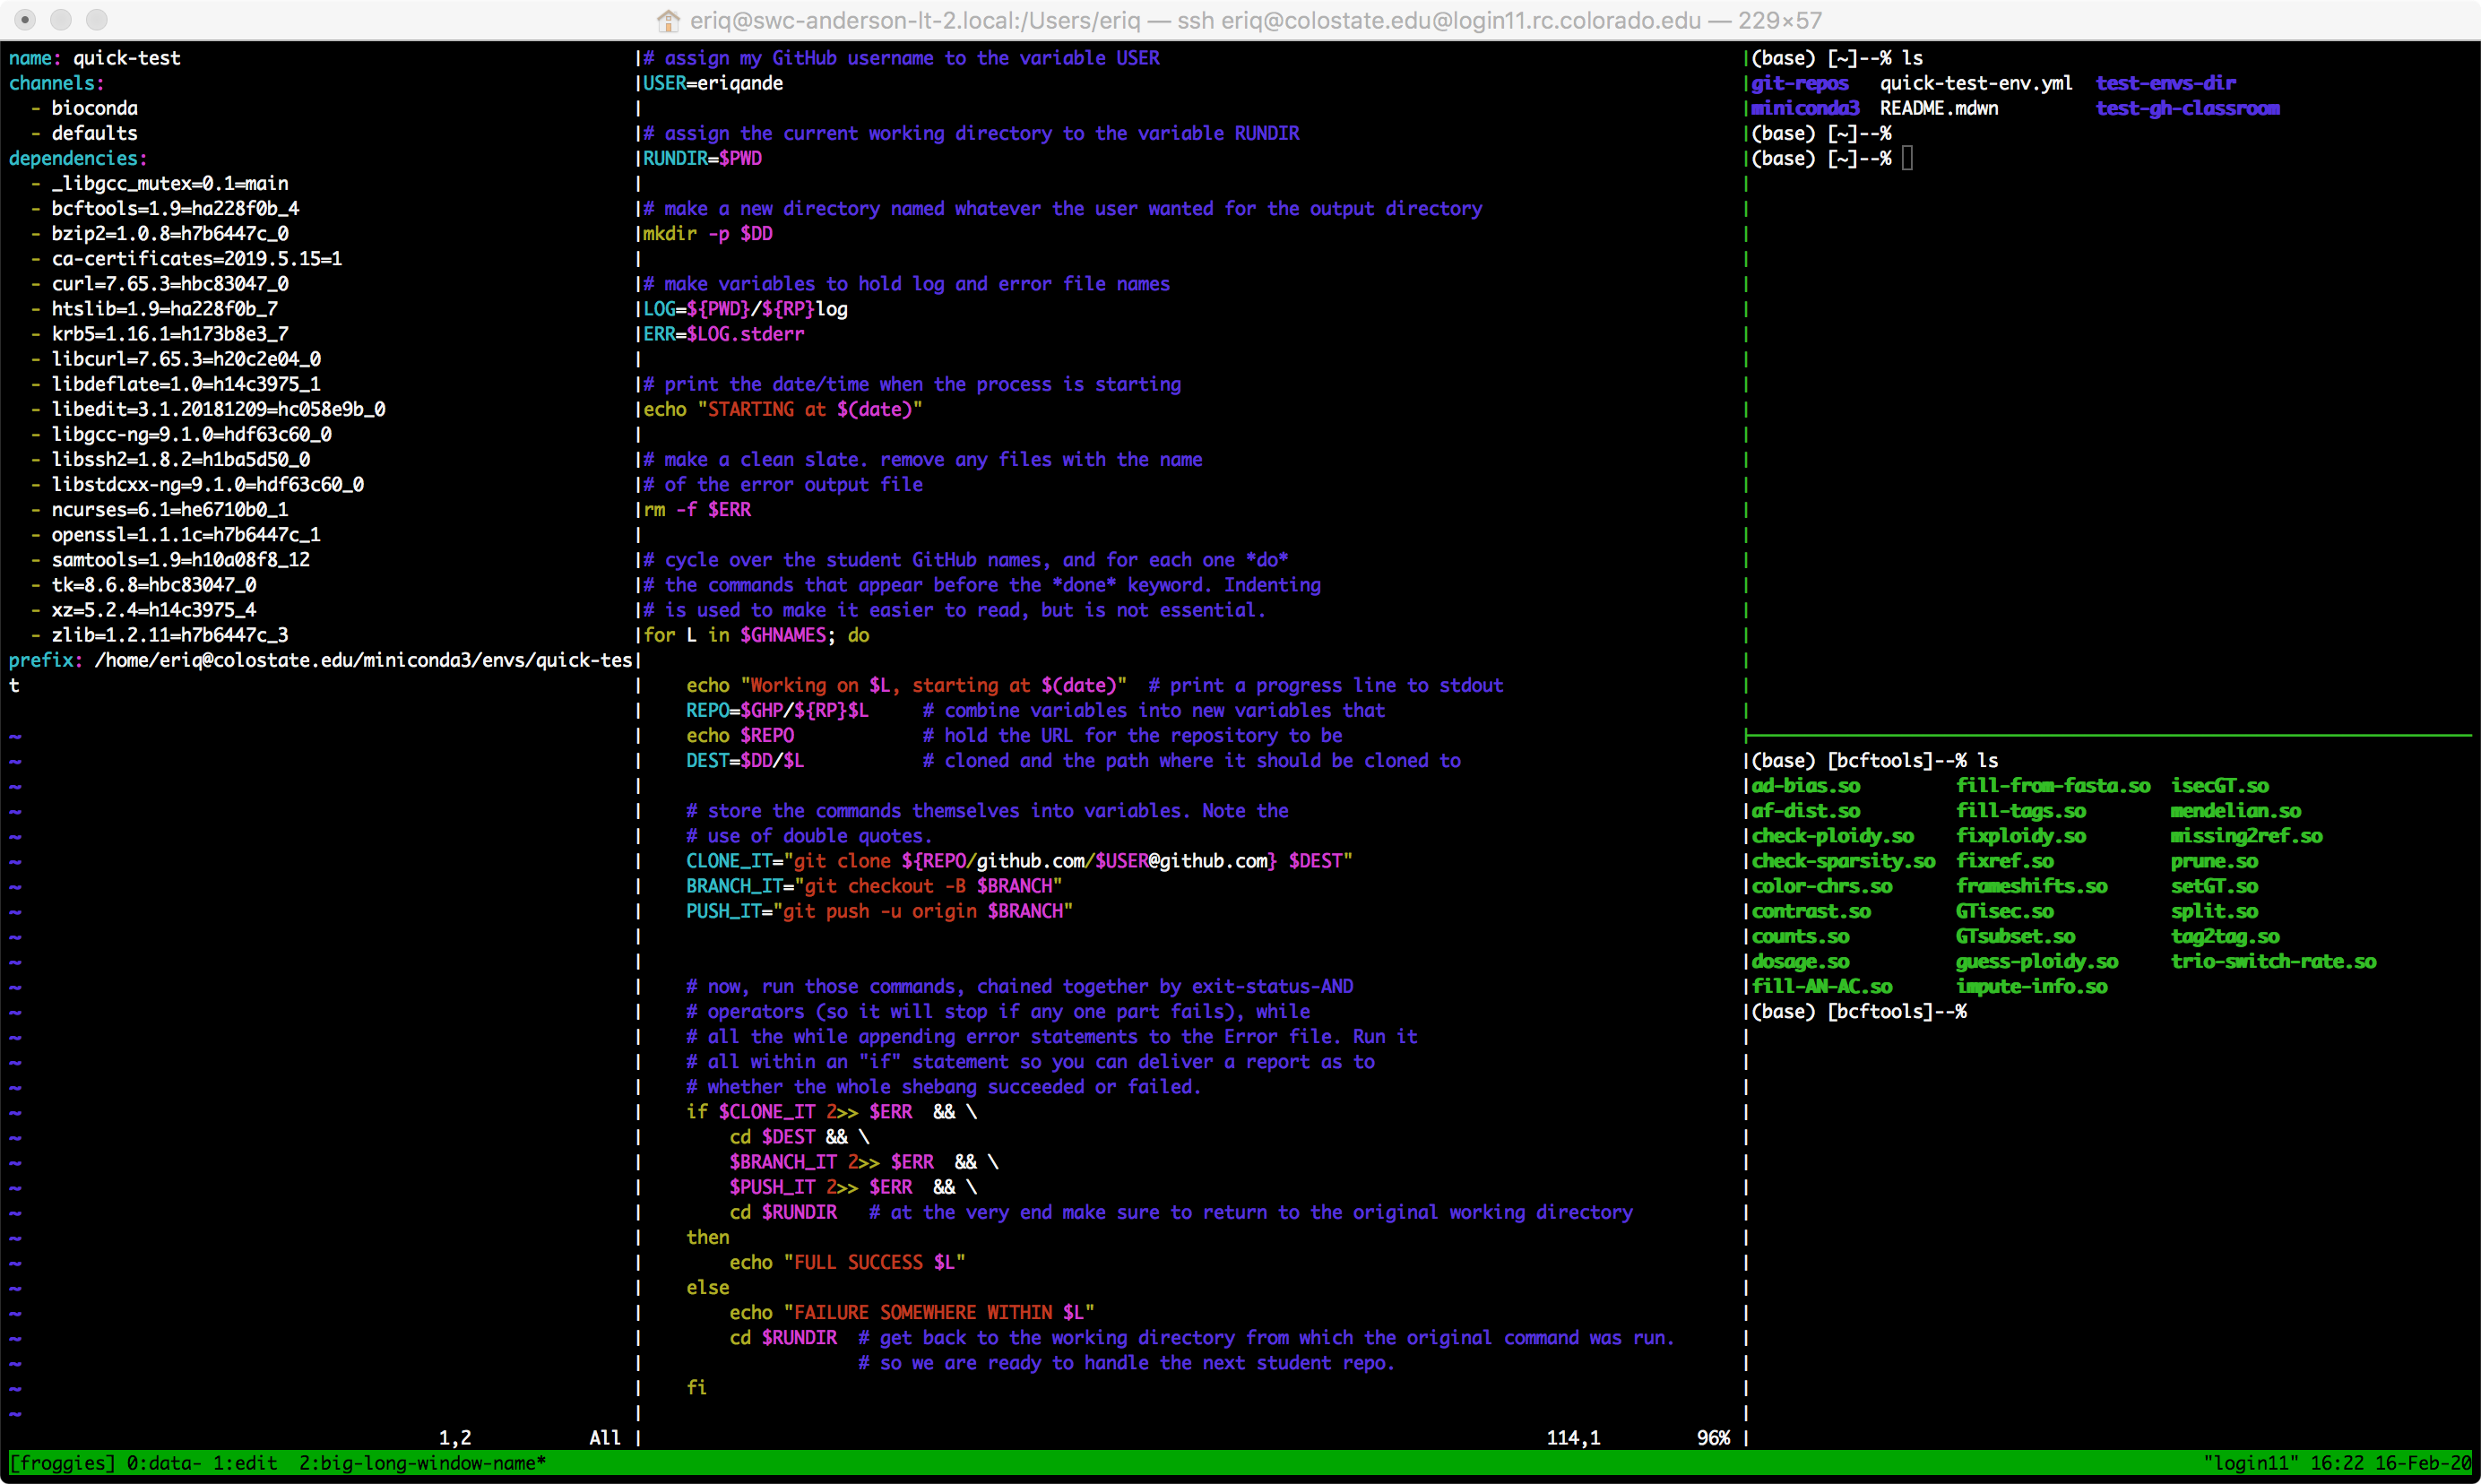
\includegraphics{figs/tmux-4-panes} 

}

\caption{A tmux window with four panes.}\label{fig:tmux-4-panes}
\end{figure}

This provides almost endless opportunities for customizing the
appearance of your terminal workspace on a remote machine for maximum
efficiency. Of course, doing so requires you know a few more
keystrokes for handling panes. These are summarized in Table \ref{tab:tmux-pane-strokes}.

\begin{longtable}[]{@{}lll@{}}
\caption{\label{tab:tmux-pane-strokes} Important keystrokes within a \texttt{tmux} session for handling panes}\tabularnewline
\toprule
\begin{minipage}[b]{0.19\columnwidth}\raggedright
Within tmux?\strut
\end{minipage} & \begin{minipage}[b]{0.25\columnwidth}\raggedright
Command\strut
\end{minipage} & \begin{minipage}[b]{0.42\columnwidth}\raggedright
Effect\strut
\end{minipage}\tabularnewline
\midrule
\endfirsthead
\toprule
\begin{minipage}[b]{0.19\columnwidth}\raggedright
Within tmux?\strut
\end{minipage} & \begin{minipage}[b]{0.25\columnwidth}\raggedright
Command\strut
\end{minipage} & \begin{minipage}[b]{0.42\columnwidth}\raggedright
Effect\strut
\end{minipage}\tabularnewline
\midrule
\endhead
\begin{minipage}[t]{0.19\columnwidth}\raggedright
Y\strut
\end{minipage} & \begin{minipage}[t]{0.25\columnwidth}\raggedright
\texttt{\textless{}cntrl\textgreater{}-b\ /}\strut
\end{minipage} & \begin{minipage}[t]{0.42\columnwidth}\raggedright
Split current window/pane
vertically into two panes\strut
\end{minipage}\tabularnewline
\begin{minipage}[t]{0.19\columnwidth}\raggedright
Y\strut
\end{minipage} & \begin{minipage}[t]{0.25\columnwidth}\raggedright
\texttt{\textless{}cntrl\textgreater{}-b\ -}\strut
\end{minipage} & \begin{minipage}[t]{0.42\columnwidth}\raggedright
Split current window/pane
horizontally into two panes\strut
\end{minipage}\tabularnewline
\begin{minipage}[t]{0.19\columnwidth}\raggedright
Y\strut
\end{minipage} & \begin{minipage}[t]{0.25\columnwidth}\raggedright
\texttt{\textless{}cntrl\textgreater{}-b\ arrow}\strut
\end{minipage} & \begin{minipage}[t]{0.42\columnwidth}\raggedright
Use \texttt{\textless{}cntrl\textgreater{}-b} + an arrow key
to move sequentially amongst
panes\strut
\end{minipage}\tabularnewline
\begin{minipage}[t]{0.19\columnwidth}\raggedright
Y\strut
\end{minipage} & \begin{minipage}[t]{0.25\columnwidth}\raggedright
\texttt{\textless{}cntrl\textgreater{}-b\ x}\strut
\end{minipage} & \begin{minipage}[t]{0.42\columnwidth}\raggedright
Kill current the current pane\strut
\end{minipage}\tabularnewline
\begin{minipage}[t]{0.19\columnwidth}\raggedright
Y\strut
\end{minipage} & \begin{minipage}[t]{0.25\columnwidth}\raggedright
\texttt{\textless{}cntrl\textgreater{}-b\ q}\strut
\end{minipage} & \begin{minipage}[t]{0.42\columnwidth}\raggedright
Paint big ID numbers (from 0
up) on the panes for a few
seconds. Hitting a number
before it disappears moves
focus to that pane.\strut
\end{minipage}\tabularnewline
\begin{minipage}[t]{0.19\columnwidth}\raggedright
Y\strut
\end{minipage} & \begin{minipage}[t]{0.25\columnwidth}\raggedright
-b {[}hjkl{]}\strut
\end{minipage} & \begin{minipage}[t]{0.42\columnwidth}\raggedright
Resize the current pane, h =
Left, j = Down, k = Up, l =
Right. It takes a while to
understand which boundary will
move.\strut
\end{minipage}\tabularnewline
\begin{minipage}[t]{0.19\columnwidth}\raggedright
Y\strut
\end{minipage} & \begin{minipage}[t]{0.25\columnwidth}\raggedright
-b z\strut
\end{minipage} & \begin{minipage}[t]{0.42\columnwidth}\raggedright
Zoom current pane to full
size. \texttt{\textless{}cntrl\textgreater{}-b\ z} again
restores it to original size.\strut
\end{minipage}\tabularnewline
\bottomrule
\end{longtable}

Now that you have seen all these keystrokes, use \texttt{\textless{}cntrl\textgreater{}-b\ \textbackslash{}} and \texttt{\textless{}cntrl\textgreater{}-b\ -} to split your windows
up into a few panes and try them out. It takes a while to get used to it, but once you get
the hang of it, it's quite nice.

\hypertarget{tmux-for-mac-users}{%
\section{\texorpdfstring{\texttt{tmux} for Mac users}{tmux for Mac users}}\label{tmux-for-mac-users}}

I put this in an entirely different section, because, if you are comfortable in
Mac-world, already, working with tmux by way of the extraordinary Mac application
\textbf{iTerm2} feels like home and it is a completely different experience than
working in \texttt{tmux} the way we have, so far.

iTerm2 is a sort of fully customizable and \emph{way} better replacement for the
standard Mac Terminal application. It can be downloaded for free
from its web page \url{https://www.iterm2.com/}. You can
donate to the project there as well. If you find that you really like iTerm2,
I recommend a donation to support the developers.

There are far too many features in iTerm2 to cover here, but I just want to describe
one very important feature: iTerm2 integration with \texttt{tmux}. If you have survived the
last section, and have gotten comfortable with hitting \texttt{\textless{}cntrl\textgreater{}-b} and then a series
of different letters to effect various changes, then that is a good thing, and will
serve you well. However, as you continue your journey with \texttt{tmux}, you may have found that
you can't scroll up through the screen the way you might be used to when working in Terminal
on a Mac. Further, you may have discovered that copying text from the screen, when you
finally figured out how to scroll up in it, involves a series of emacs-like keystrokes.
This is fine if you are up for it, but it is understandable that a Mac user might yearn
for a more Mac-like experience. Fortunately, the developers of iTerm2 have made your tmux experience
much better! They exploit \texttt{tmux}'s \texttt{-CC} option, which puts \texttt{tmux} into ``control mode'' such that
iTerm2 can send its own simple text commands to control \texttt{tmux}, rather than the user sending
commands prefaced by \texttt{\textless{}cntrl\textgreater{}-b}. The consequence of this is that iTerm2 has a series of menu options
for doing \texttt{tmux} actions, and all of these have keyboard shortcuts that seem more natural to
a Mac user. You can establish sessions, open new windows (as tabs in iTerm, if desired) and
even carve windows up into multiple panels---all from a Mac-style interface that is quite forgiving
in case you happen to forget the exact key sequence to do something in \texttt{tmux}.
Finally, using \texttt{tmux} via iTerm2 you get mouse interaction like you expect: you can use the
mouse to select different panes and move the dividers between them, and you can scroll back
and select text with the mouse, if desired.

On top of that, iTerm2 has great support for creating different profiles that you can
assign to different remote servers. These can be customized with different login actions
(including storage of remote server passwords in the Apple keychain, so you don't have
to type in your long, complex passwords every time you log in to a remote server you
can't set a public/private keypair on), and with different color schemes that can help you
to keep various windows attached to various remote servers straight.

You can read about it all at the iTerm2 website. I will just add that using
iTerm with \texttt{tmux} might require a later version of \texttt{tmux} than is installed
on your remote server or cluster. I recommend that you use Miniconda (see Section \ref{miniconda})
to install tmux version 2.9 into your base environment with \texttt{conda\ install\ -c\ conda-forge\ tmux=2.9}.
Before you do that, be sure to kill all existing tmux sessions on your remote server.
Then, you could make a profile named, say \texttt{summit-tmux}, that launched with a command
that was like this:

\begin{Shaded}
\begin{Highlighting}[]
\FunctionTok{ssh}\NormalTok{ -t eriq@colostate.edu@login11.rc.colorado.edu }\StringTok{"/projects/eriq@colostate.edu/miniconda3/bin/tmux -CC attach -t summit || /projects/eriq@colostate.edu/miniconda3/bin/tmux -CC new -s summit"}
\end{Highlighting}
\end{Shaded}

But customized to your own account name. What that does when you open a \texttt{summit-tmux} session is
\texttt{ssh} to SUMMIT, and immediately run the command in the double quotes. That command says,
``try to attach to a \texttt{tmux} session named \texttt{summit}. If that fails, then create a new
\texttt{tmux} session called \texttt{summit}.'' To get the password manager set up for that profile,
you need to add to the password manager an account (call it \texttt{summit}) and store your summit
password in that manager. Then, in your summit-tmux profile, set a trigger (Profile-\textgreater{}Advanced-\textgreater{}Triggers (Edit))
which looks for the regular expression \texttt{\^{}Password:}, does the action ``Open Password Manager'', and does so
instantly. Figure \ref{fig:iterm-trigger} is a screen shot of what that setup looks like in my SUMMIT profile:

\begin{figure}
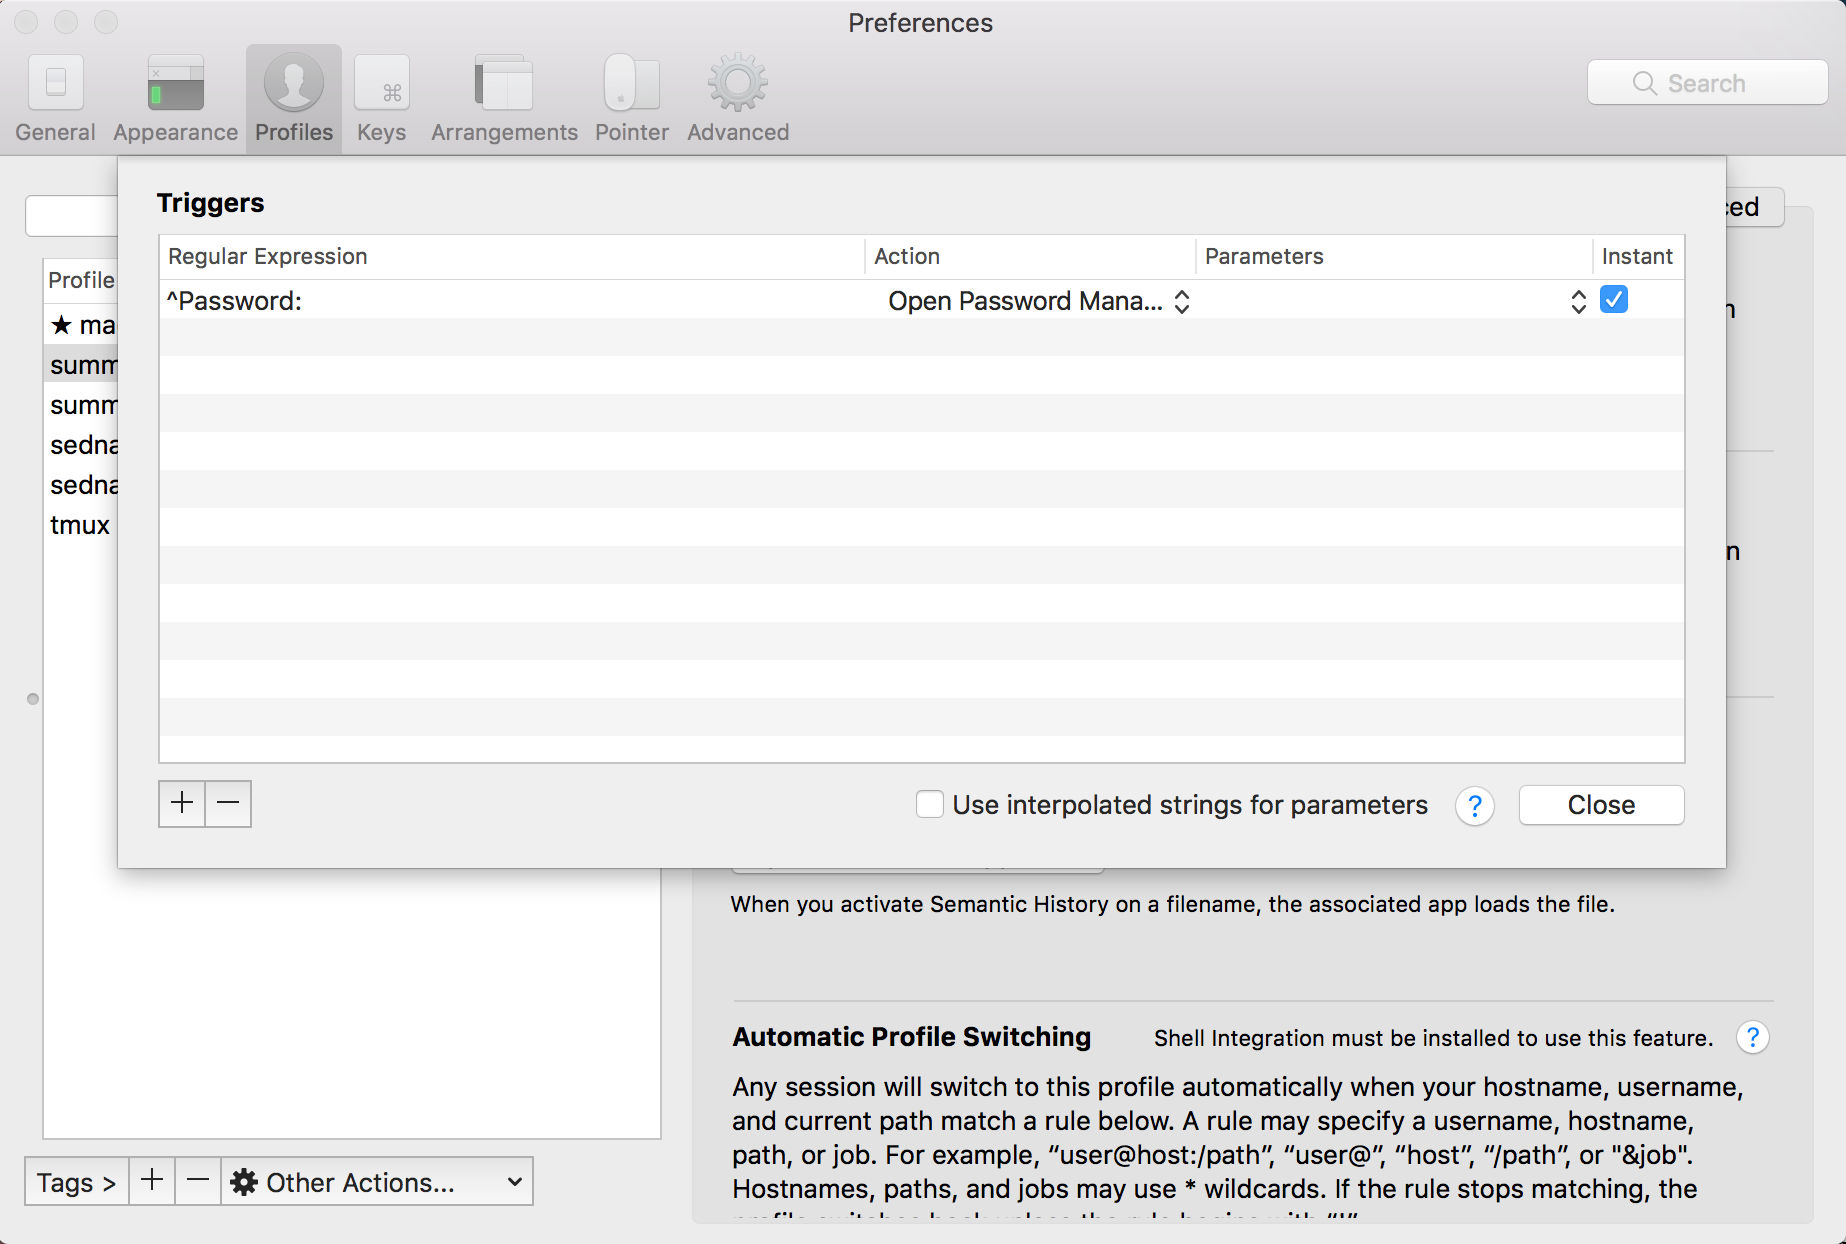
\includegraphics[width=25.64in]{figs/iterm-pw-trigger} \caption{How to set a trigger to open the password manager in iTerm to be able to pass in your password.  This is telling iTerm to open the Password Manager whenever it finds `Password:` at the beginning of a line in the terminal.}\label{fig:iterm-trigger}
\end{figure}

If you are a Mac user, spend a weekend getting to know iTerm2. It will be time well spent.

\hypertarget{installing-software-on-an-hpcc}{%
\section{Installing Software on an HPCC}\label{installing-software-on-an-hpcc}}

In order to do anything useful on a remote computer or a
high-performance computing cluster (called a ``cluster'' or an ``HPCC'')
you will need to have software programs
for analyzing data. As we have seen, a lot of the nuts and bolts of writing command
lines uses utilities that are found on every Unix computer. However almost always
your bioinformatic analyses will require programs or software that
do not come ``standard'' with Unix. For example, the specialized programs for
sequence assembly and alignment will have to be \emph{installed} on the cluster
in order for you to be able to use them.

It turns out that installing software on a Unix machine (or cluster) has not
always been a particularly easy thing to do for a number or reasons. First, for
a long time, Unix software was largely distributed in the form of \emph{source code}: the
actual programming code (text) written by the developers that describes the actions
that a program takes. Such computer code cannot be run directly, it first must be
\emph{compiled} into a \emph{binary} or \emph{executable} program. Doing this can be a challenging
process. First, computer code compilation can be very time consuming (if you use R
on Linux, and install all your packages from CRAN---which requires compilation---you
will know that!). Secondly, vexing errors and failures can occur when the
compiler or the computer architecture is in conflict with the program code. (I have lost
entire days trying to solve compiling problems). On top of that, in order to run, most
programs do not operate in a standalone fashion; rather, while a program is running, it
typically depends on computer code and routines that must be stored in separate \emph{libraries} on your
Unix computer. These libraries are known as program \emph{dependencies}. So, installing a program
requires not just installing the program itself, but also ensuring that the program's dependencies
are installed \emph{and} that the program knows where they are installed. As if that were not enough,
the dependencies of some programs can conflict (be incompatible) with the dependencies of other
programs, and particular versions of a program might require particular versions of
the dependencies. Additionally, some versions of some programs might not work with particular
versions (types of chips) of some computer systems. Finally, most systems for installing
software that were in place on Unix
machines a decade ago required that whoever was installing software have \emph{administrative privileges}
on the computer. On an HPCC, none of the typical users have administrative privileges which are,
as you might guess, reserved for the system administrators.

For all the reasons above, installing software on an HPCC used to be a harrowing
affair: you either had to be fluent in compilers and libraries to do it yourself in your
home directory or you had to beg your system administrator. (Though our cluster computing
sysadmins at NMFS are wonderful, that is not always the case\ldots{}\href{https://www.wiw.org/~chris/archive/dilbert/}{see Dilbert}).
On HPCC's the system administrators have to contend with requests from multiple users
for different software and different versions. They solve this (somewhat headachey)
problem by installing software into separate ``compartments'' that allow different software
and versions to be maintained on the system without all of it being accessible at once.
Doing so, they create \emph{modules} of software. This is discussed in the following section.

Today, however, a large group of motivated people have created a software management
system called Miniconda that tries to solve many of the problems encountered in maintaining
software on a computer system. First, Miniconda maintains a huge repository of
programs that are already \emph{pre-compiled} for a number of different chip architectures, so that
programs can usually be installed without the time-consuming compiling process. Second, the repository
maintains critical information on the dependencies for each software program, and about
conflicts and incompatibilities between different versions of programs, architectures and
dependencies. Third, the Miniconda system is built from the ground up to make it easy to maintain
separate software \emph{environments} on your system. These different environments have different
software programs or different versions of different software programs. Such an approach
was originally used so developers could use a single computer to test any new code
they had written in a number of different
computing environments; however, it has become an incredibly valuable tool for ensuring
that your analyses are reproducible: you can give people not just the data and scripts that you
used for the analysis, but also the computing/software environment (with all the same
software versions) that you used for the analysis. And, finally, all of this
can be done with Miniconda without have administrative privileges. Effectively,
Miniconda manages all these software programs and dependencies \emph{within your home directory}.
Section \ref{miniconda} provides details about Miniconda and describes how to use it
to install bioinformatics software.

\hypertarget{modules}{%
\subsection{Modules}\label{modules}}

(not written)

This is if your sys admin has made it easy.

The big point I must make here is that these don't work like conda environments.
Environments are ``all-or-nothing,'' whereas modules are ``cumulative'' and can be
layered atop one another. (If doing so creates conflicts, then the sysadmins have to
figure that out\ldots{}perhaps this is one reason that modules will often carry older (if not
completely antiquated) versions of software.)

\hypertarget{miniconda}{%
\subsection{Miniconda}\label{miniconda}}

We will first walk you through a few steps with Miniconda to install some
bioinformatic software into an environment on your cluster. After that we will discuss more about
the underlying philosophy of Miniconda, and how it is operating.

\hypertarget{installing-or-updating-miniconda}{%
\subsubsection{Installing or updating Miniconda}\label{installing-or-updating-miniconda}}

\begin{enumerate}
\def\labelenumi{\arabic{enumi}.}
\item
  To do installation of software, you probably should not be on SUMMIT's login nodes.
  They offer ``compile nodes'' that should be suitable for installing with Miniconda. So, do this:

\begin{Shaded}
\begin{Highlighting}[]
\FunctionTok{ssh}\NormalTok{ scompile}
\end{Highlighting}
\end{Shaded}
\item
  If you are on Hummingbird, be sure to get a \texttt{bash} shell before doing anything else, by typing \texttt{bash}
  (if you have not already set \texttt{bash} as your default shell (see the previous chapter)).
\item
  First, check if you have Miniconda. Update it if you do, and install it if you don't:

\begin{Shaded}
\begin{Highlighting}[]
\CommentTok{# just type conda at the command line:}
\ExtensionTok{conda}
\end{Highlighting}
\end{Shaded}

  If you see some help information, then you already have Miniconda (or Anaconda) and you
  should merely update it with:

\begin{Shaded}
\begin{Highlighting}[]
\ExtensionTok{conda}\NormalTok{ update conda}
\end{Highlighting}
\end{Shaded}

  If you get an error telling you that your computer does not know about a command, \texttt{conda}, then
  you do not have Miniconda and you must install it. You do that by downloading the Miniconda package
  with \texttt{wget} and then running the Miniconda installer, like this:

\begin{Shaded}
\begin{Highlighting}[]
\CommentTok{# start in your home directory and do the following:}
\FunctionTok{mkdir}\NormalTok{ conda_install}
\BuiltInTok{cd}\NormalTok{ conda_install/}
\FunctionTok{wget}\NormalTok{ https://repo.anaconda.com/miniconda/Miniconda3-latest-Linux-x86_64.sh}
\FunctionTok{chmod}\NormalTok{ u+x Miniconda3-latest-Linux-x86_64.sh }
\ExtensionTok{./Miniconda3-latest-Linux-x86_64.sh} 
\end{Highlighting}
\end{Shaded}

  That launches the Miniconda installer (it is a shell script). Follow the prompts and agree
  to the license and to the default install location and to initialize conda.
  At the end, it tells you to log out of your shell and log back in for changes to take
  effect. It turns out that it suffices to do \texttt{cd\ \textasciitilde{};\ source\ .bash\_profile}
\end{enumerate}

Once you complete the above, your command prompt should have been changed to something that looks like:

\begin{Shaded}
\begin{Highlighting}[]
\KeywordTok{(}\ExtensionTok{base}\KeywordTok{)}\NormalTok{ [}\ExtensionTok{~}\NormalTok{]}\ExtensionTok{--%}
\end{Highlighting}
\end{Shaded}

The \texttt{(base)} is telling you that you are in Miniconda's \emph{base} environment. Typically you want to keep the
\emph{base} environment clean of installed software, so we will install software into a new environment.

\hypertarget{installing-software-into-a-bioinformatics-environment}{%
\subsubsection{Installing software into a bioinformatics environment}\label{installing-software-into-a-bioinformatics-environment}}

If everything went according to plan above, then we are ready to use Miniconda to
install some software for bioinformatics. We will install a few programs that we will
use extensively in the next few weeks: \texttt{bwa}, \texttt{samtools}, and \texttt{bcftools}. We will
install these programs into a conda environment that we will name \texttt{bioinf} (short
for ``bioinformatics''). It takes just a single command:

\begin{Shaded}
\begin{Highlighting}[]
\ExtensionTok{conda}\NormalTok{ create -n bioinf -c bioconda bwa samtools bcftools}
\end{Highlighting}
\end{Shaded}

That should only take a few seconds.

To test that we got the programs we must \emph{activate} the \texttt{bioinf} environment, and then issue
the commands, \texttt{bwa}, \texttt{samtools}, and \texttt{bcftools}. Each of those should spit back some help
information. If so, that means they are installed correctly! It looks like this:

\begin{Shaded}
\begin{Highlighting}[]
\ExtensionTok{conda}\NormalTok{ activate bioinf}
\end{Highlighting}
\end{Shaded}

After that you should get a command prompt that starts with \texttt{(bioinf)}, telling you that the
active conda environment is \texttt{bioinf}. Now, try these commands:

\begin{Shaded}
\begin{Highlighting}[]
\ExtensionTok{bwa}
\ExtensionTok{samtools}
\ExtensionTok{bcftools}
\end{Highlighting}
\end{Shaded}

\hypertarget{uninstalling-miniconda-and-its-associated-environments}{%
\subsubsection{Uninstalling Miniconda and its associated environments}\label{uninstalling-miniconda-and-its-associated-environments}}

It may become necessary at some point to uninstall Miniconda. One important case of this
is if you end up overflowing your home directory with conda-installed software. In this case,
unless you have installed numerous, complex environments, the simplest thing to do is
to ``uninstall'' Miniconda, reinstall it in a location with fewer hard-drive space constraints,
and then simply recreate the environments you need, as you did originally.

This is actually quite germane to SUMMIT users. The size quota on home directories on SUMMIT is
only 2 Gb, so you can easily fill up your home directory by installing a few conda environments.
To check how much of the hard
drive space allocated to you is in use on SUMMIT, use the \texttt{curc-quota} command. (Check the documentation
for how to check space on other HPCCs, but note that Hummingbird users get 1 TB on their home
directories). Instead of
using your home directory to house your Miniconda software, on SUMMIT you can put it in your
\texttt{projects} storage area. Each user gets more storage (like 250 Gb) in a directory
called \texttt{/projects/username} where \texttt{username} is replaced by your SUMMIT username,
for example: \texttt{/projects/eriq@colostate.edu}

To ``uninstall'' Miniconda, you first must delete the \texttt{miniconda3} directory in your
home directory (if that is where it got installed to). This can take a while. It is done with:

\begin{Shaded}
\begin{Highlighting}[]
\FunctionTok{rm}\NormalTok{ -rf ~/miniconda3}
\end{Highlighting}
\end{Shaded}

Then you have to delete the lines between \texttt{\#\ \textgreater{}\textgreater{}\textgreater{}} and \texttt{\#\ \textless{}\textless{}\textless{}}, wherever they occur in your \texttt{\textasciitilde{}/.bashrc} and \texttt{\textasciitilde{}/bash\_profile}
files, i.e., you will have to remove all of the lines that look
something like thius:

\begin{Shaded}
\begin{Highlighting}[]
\CommentTok{# >>> conda initialize >>>}
\CommentTok{# !! Contents within this block are managed by 'conda init' !!}
\VariableTok{__conda_setup=}\StringTok{"}\VariableTok{$(}\StringTok{'/Users/eriq/miniconda3/bin/conda'} \StringTok{'shell.bash'} \StringTok{'hook'} \OperatorTok{2>} \ExtensionTok{/dev/null}\VariableTok{)}\StringTok{"}
\KeywordTok{if}\BuiltInTok{ [} \VariableTok{$?} \OtherTok{-eq}\NormalTok{ 0}\BuiltInTok{ ]}\NormalTok{; }\KeywordTok{then}
    \BuiltInTok{eval} \StringTok{"}\VariableTok{$__conda_setup}\StringTok{"}
\KeywordTok{else}
    \KeywordTok{if}\BuiltInTok{ [} \OtherTok{-f} \StringTok{"/Users/eriq/miniconda3/etc/profile.d/conda.sh"}\BuiltInTok{ ]}\NormalTok{; }\KeywordTok{then}
        \BuiltInTok{.} \StringTok{"/Users/eriq/miniconda3/etc/profile.d/conda.sh"}
    \KeywordTok{else}
        \BuiltInTok{export} \VariableTok{PATH=}\StringTok{"/Users/eriq/miniconda3/bin:}\VariableTok{$PATH}\StringTok{"}
    \KeywordTok{fi}
\KeywordTok{fi}
\BuiltInTok{unset} \VariableTok{__conda_setup}
\CommentTok{# <<< conda initialize <<<}
\end{Highlighting}
\end{Shaded}

After all those conda lines are removed from your \texttt{\textasciitilde{}/.bashrc} and \texttt{\textasciitilde{}/bash\_profile}, logging out
and logging back in, you should be free from conda and ready to reinstall it in
a different location.

To reinstall miniconda in a different location, just follow the
installation instructions above, but when you are running the
\texttt{./Miniconda3-latest-Linux-x86\_64.sh} script, instead of choosing the default
install location, use a location in your project directory. For example, for me, that is:
\texttt{/projects/eriq@colostate.edu/miniconda3}.

Then, recreate the \texttt{bioinf} environment described above.

If you are having fun making environments and you think that you might like to use R on
the cluster, then you might want to make an environment with some bioinformatics software
that also has
the latest version of R on miniconda installed. At the time of writing that was R 3.6.1. So,
do:

\begin{Shaded}
\begin{Highlighting}[]
\ExtensionTok{conda}\NormalTok{ create -n binfr -c bioconda bwa samtools bcftools r-base=3.6.1 r-essentials}
\end{Highlighting}
\end{Shaded}

That makes an environment called \texttt{binfr} (which turns out to also be \textbf{way} easier to type that \texttt{bioinfr}).
The \texttt{r-essentials} in the above command line is the name for a collection of 200 commonly used R packages (including
the \texttt{tidyverse}). This procedure takes a little while, but it is still far less painful than using the
version of R that is installed on SUMMIT with the \texttt{modules} packages, and then trying to build the tidyverse
from source with \texttt{install.packages()}.

\hypertarget{what-is-miniconda-doing}{%
\subsubsection{What is Miniconda doing?}\label{what-is-miniconda-doing}}

This is a good question. We won't go deeply into the specifics, but will skim the
surface of a few topics that can help you understand what Miniconda is doing.

First, Miniconda is downloading programs and their dependencies into the \texttt{miniconda3}
directory. Based on the lists of dependencies and conflicts for each program that is being
installed, it makes a sort of ``equation,'' which it can ``solve'' to find the versions of
different programs and libraries that can be installed and which should ``play nicely with
one another (and with your specific computer architecture.'' While it is solving this
``equation'' it is doing so while also doing its best
to optimize features of the programs (like using the latest versions, if possible).
Solving this ``equation'' is an example of a Boolean Satisfiability problem, which is a known
class of difficult (time-consuming) problems. If you are requesting a lot of programs, and
especially if you do not constrain your request (by demanding a certain version of
the program) then ``solving'' the request may take a long time. However, when installing
just a few bioinformatics programs it is unlikely to ever take too terribly long.

Once miniconda has decided on which versions of which programs and dependencies to install,
it downloads them and then places them into the requested environment (or the active environment
if no environment is specifically requested). If a program is installed into an environment, then you
can access that program by activating the environment (i.e. \texttt{conda\ activate\ bioinf}). Importantly,
if you don't activate the environment, you won't be able to use the programs installed there.
We will see later in writing bioinformatic scripts, you will always have to explicitly
activate a desired conda environment when you run a script on a compute node through the job
scheduler.

The way that Miniconda delivers programs in an environment is by storing all the programs
in a special environment directory (within the \texttt{miniconda3/envs} directory), and then, when
the environment is activated, the main thing that is happening is that \texttt{conda} is manipulating your
PATH variable to include directories within the environment's directory
within the \texttt{miniconda3/envs} directory. An easy way to see this is simply by
inspecting your path variable while in different environments. Here we compare the PATH
variable in the \texttt{base} environment, versus in the \texttt{bioinf} environment, versus in the
\texttt{binfr} environment:

\begin{Shaded}
\begin{Highlighting}[]
\KeywordTok{(}\ExtensionTok{base}\KeywordTok{)}\NormalTok{ [}\ExtensionTok{~}\NormalTok{]}\ExtensionTok{--%}\NormalTok{ echo }\VariableTok{$PATH}
\ExtensionTok{/projects/eriq@colostate.edu/miniconda3}\NormalTok{/bin:}\ExtensionTok{/projects/eriq@colostate.edu/miniconda3}\NormalTok{/condabin:}\ExtensionTok{/usr/local}\NormalTok{/bin:/bin:}\ExtensionTok{/usr}\NormalTok{/bin:}\ExtensionTok{/usr}\NormalTok{/bin:}\ExtensionTok{/usr/local}\NormalTok{/sbin:}\ExtensionTok{/usr}\NormalTok{/sbin:}\ExtensionTok{/home/eriq@colostate.edu}\NormalTok{/bin:}\ExtensionTok{/home/eriq@colostate.edu/bin}
\KeywordTok{(}\ExtensionTok{base}\KeywordTok{)}\NormalTok{ [}\ExtensionTok{~}\NormalTok{]}\ExtensionTok{--%}\NormalTok{ conda activate bioinf}
\KeywordTok{(}\ExtensionTok{bioinf}\KeywordTok{)}\NormalTok{ [}\ExtensionTok{~}\NormalTok{]}\ExtensionTok{--%}\NormalTok{ echo }\VariableTok{$PATH}
\ExtensionTok{/projects/eriq@colostate.edu/miniconda3/envs/bioinf}\NormalTok{/bin:}\ExtensionTok{/projects/eriq@colostate.edu/miniconda3}\NormalTok{/condabin:}\ExtensionTok{/usr/local}\NormalTok{/bin:/bin:}\ExtensionTok{/usr}\NormalTok{/bin:}\ExtensionTok{/usr}\NormalTok{/bin:}\ExtensionTok{/usr/local}\NormalTok{/sbin:}\ExtensionTok{/usr}\NormalTok{/sbin:}\ExtensionTok{/home/eriq@colostate.edu}\NormalTok{/bin:}\ExtensionTok{/home/eriq@colostate.edu/bin}
\KeywordTok{(}\ExtensionTok{bioinf}\KeywordTok{)}\NormalTok{ [}\ExtensionTok{~}\NormalTok{]}\ExtensionTok{--%}\NormalTok{ conda activate binfr}
\KeywordTok{(}\ExtensionTok{binfr}\KeywordTok{)}\NormalTok{ [}\ExtensionTok{~}\NormalTok{]}\ExtensionTok{--%}\NormalTok{ echo }\VariableTok{$PATH}
\ExtensionTok{/projects/eriq@colostate.edu/miniconda3/envs/binfr}\NormalTok{/bin:}\ExtensionTok{/projects/eriq@colostate.edu/miniconda3}\NormalTok{/condabin:}\ExtensionTok{/usr/local}\NormalTok{/bin:/bin:}\ExtensionTok{/usr}\NormalTok{/bin:}\ExtensionTok{/usr}\NormalTok{/bin:}\ExtensionTok{/usr/local}\NormalTok{/sbin:}\ExtensionTok{/usr}\NormalTok{/sbin:}\ExtensionTok{/home/eriq@colostate.edu}\NormalTok{/bin:}\ExtensionTok{/home/eriq@colostate.edu/bin}
\end{Highlighting}
\end{Shaded}

(To be sure, \texttt{miniconda} can change a few more things than just your PATH variable when you activate an environment, but
for the typical user, the changes to PATH are most important.)

\hypertarget{what-programs-are-available-on-minconda}{%
\subsubsection{What programs are available on Minconda?}\label{what-programs-are-available-on-minconda}}

There are quite a few programs for multiple platforms. If you are wondering
whether a particular program is available from Miniconda, the easiest first
step is to Google it. For example, search for \texttt{miniconda\ bowtie}.

You can also search from the command line using \texttt{conda\ search}. Note that most
bioinformatics programs you will be interested in are available on a conda
\emph{channel} called \texttt{bioconda}. You probably saw the \texttt{-c\ bioconda} option
applied to the \texttt{conda\ create} commands above. That options tells conda to search
the Bioconda channel for programs and packages.

Here, you can try searching for a couple of packages that you might
end up using to analyze genomic data:

\begin{Shaded}
\begin{Highlighting}[]
\ExtensionTok{conda}\NormalTok{ search -c bioconda plink}

\CommentTok{# and next:}

\ExtensionTok{conda}\NormalTok{ search -c bioconda angsd}
\end{Highlighting}
\end{Shaded}

\hypertarget{can-i-add-more-programs-to-an-environment}{%
\subsubsection{Can I add more programs to an environment?}\label{can-i-add-more-programs-to-an-environment}}

This is a worthwhile question. Imagine that we have been happily working in our \texttt{bioinf} conda environment
for a few months. We have finished all our tasks with \texttt{bwa}, \texttt{samtools}, and \texttt{bcftools}, but perhaps now we
want to analyze some of the data with \texttt{angsd} or \texttt{plink}. Can we add those programs to our
\texttt{bioinf} environment? The short answer is ``Yes!''. The steps are easy.

\begin{enumerate}
\def\labelenumi{\arabic{enumi}.}
\item
  Activate the environment you wish to add the programs to (i.e. \texttt{conda\ activate\ bioinf} for example).
\item
  Then use \texttt{conda\ install}. For example to install specific versions of \texttt{plink} and \texttt{angsd} that we
  saw above while searching for those packages we might do:

\begin{Shaded}
\begin{Highlighting}[]
\ExtensionTok{conda}\NormalTok{ install -c bioconda plink=1.90b6.12 angsd=0.931}
\end{Highlighting}
\end{Shaded}
\end{enumerate}

Now, the longer answer is ``Yes, but\ldots{}'' The big ``but'' there occurs because if different
programs require the same dependencies, but rely on different versions of the dependencies,
installing programs over different commands can cause miniconda to not identify some
incompatibilities between program dependencies. A germane example occurs if you first install
\texttt{samtools} into an environment, and then, after that, you install \texttt{bcftools}, like this:

\begin{Shaded}
\begin{Highlighting}[]
\ExtensionTok{conda}\NormalTok{ create -n samtools-first        # create an empty environment}
\ExtensionTok{conda}\NormalTok{ activate samtools-first         # activate the environment}
\ExtensionTok{conda}\NormalTok{ install -c bioconda samtools    # install samtools}
\ExtensionTok{conda}\NormalTok{ install -c bioconda bcftools    # install bcftools}
\ExtensionTok{bcftools}\NormalTok{                              # try running bcftools}
\end{Highlighting}
\end{Shaded}

When you try running the last line, \texttt{bcftools} barfs on you like so:

\begin{Shaded}
\begin{Highlighting}[]
\ExtensionTok{bcftools}\NormalTok{: error while loading shared libraries: libcrypto.so.1.0.0: cannot open shared object file: No such file or directory}
\end{Highlighting}
\end{Shaded}

So, often, installing extra programs does not create problems, but it can. If you find yourself battling
errors from conda-installed programs, see if you can correct that by creating a new environment and installing all the programs
you want at the same time, in one fell swoop, using \texttt{conda\ create}, as in:

\begin{Shaded}
\begin{Highlighting}[]
\ExtensionTok{conda}\NormalTok{ create -n binfr -c bioconda bwa samtools bcftools r-base=3.6.1 r-essentials}
\end{Highlighting}
\end{Shaded}

\hypertarget{exporting-environments}{%
\subsubsection{Exporting environments}\label{exporting-environments}}

In our introduction to Miniconda, we mentioned that it is a great boon to
reproducibility. Clearly, your analyses will be more reproducible if it is
easier for others to install software to repeat your analyses. However, Miniconda
takes that one step further, allowing you to generate a list of
the specific versions of
all software and dependencies in a conda environment. This list is a complete
record of your environment, and, supplied to conda, it is a specification of
exactly how to recreate that environment.

The process of creating such a list is called \emph{exporting} the conda
environment. Here we demonstrate its use by exporting the \texttt{bioinf}
environment from SUMMIT to a simple text file. Then we use that text file
to recreate the environment on my laptop.

\begin{Shaded}
\begin{Highlighting}[]
\CommentTok{# on summit:}
\ExtensionTok{conda}\NormalTok{ activate bioinf          # activate the environment}
\ExtensionTok{conda}\NormalTok{ env export               # export the environment}
\end{Highlighting}
\end{Shaded}

The last command above just sends the exported environment
to stdout, looking like this:

\begin{verbatim}
name: bioinf
channels:
  - bioconda
  - defaults
dependencies:
  - _libgcc_mutex=0.1=main
  - bcftools=1.9=ha228f0b_4
  - bwa=0.7.17=hed695b0_7
  - bzip2=1.0.8=h7b6447c_0
  - ca-certificates=2020.1.1=0
  - curl=7.68.0=hbc83047_0
  - htslib=1.9=ha228f0b_7
  - krb5=1.17.1=h173b8e3_0
  - libcurl=7.68.0=h20c2e04_0
  - libdeflate=1.0=h14c3975_1
  - libedit=3.1.20181209=hc058e9b_0
  - libgcc-ng=9.1.0=hdf63c60_0
  - libssh2=1.8.2=h1ba5d50_0
  - libstdcxx-ng=9.1.0=hdf63c60_0
  - ncurses=6.1=he6710b0_1
  - openssl=1.1.1d=h7b6447c_4
  - perl=5.26.2=h14c3975_0
  - samtools=1.9=h10a08f8_12
  - tk=8.6.8=hbc83047_0
  - xz=5.2.4=h14c3975_4
  - zlib=1.2.11=h7b6447c_3
prefix: /projects/eriq@colostate.edu/miniconda3/envs/bioinf
\end{verbatim}

The format of this information is YAML (Yet Another Markup Language),
(which we saw in the headers of RMarkdown documents, too).

If we stored that output in a file:

\begin{Shaded}
\begin{Highlighting}[]
\ExtensionTok{conda}\NormalTok{ env export }\OperatorTok{>}\NormalTok{ bioinf.yml}
\end{Highlighting}
\end{Shaded}

And then copied that file to another computer, then we can recreate
the environment on that other computer with:

\begin{Shaded}
\begin{Highlighting}[]
\ExtensionTok{conda}\NormalTok{ env create -f bioinf.yml}
\end{Highlighting}
\end{Shaded}

That should work fine if the new computer is of the same architecture (i.e., both
are Linux computers, or both are Macs). However, the specific build numbers
referenced in the YAML (i.e.~things like the \texttt{h7b6447c\_3} part of the program name)
can create problems when installing on other architectures. In that case, we must
export without the build names:

\begin{Shaded}
\begin{Highlighting}[]
\ExtensionTok{conda}\NormalTok{ env export --no-builds }\OperatorTok{>}\NormalTok{ bioinf.yml}
\end{Highlighting}
\end{Shaded}

Even that might fail if the dependencies differ on different architectures,
in which case you can export just the list of the actual programs that
you reqested be installed, by using the \texttt{-\/-from-history} option. For example:

\begin{Shaded}
\begin{Highlighting}[]
\ExtensionTok{%}\NormalTok{ conda env export --from-history}
\ExtensionTok{name}\NormalTok{: bioinf}
\ExtensionTok{channels}\NormalTok{:}
  \ExtensionTok{-}\NormalTok{ defaults}
\ExtensionTok{dependencies}\NormalTok{:}
  \ExtensionTok{-}\NormalTok{ bwa}
  \ExtensionTok{-}\NormalTok{ bcftools}
  \ExtensionTok{-}\NormalTok{ samtools}
\ExtensionTok{prefix}\NormalTok{: /projects/eriq@colostate.edu/miniconda3/envs/bioinf}
\end{Highlighting}
\end{Shaded}

Though, even that fails, cuz it doesn't list bioconda in there.

\hypertarget{vim-its-time-to-get-serious-with-text-editing}{%
\section{\texorpdfstring{\texttt{vim}: it's time to get serious with text editing}{vim: it's time to get serious with text editing}}\label{vim-its-time-to-get-serious-with-text-editing}}

Introduce newbs to the \texttt{vimtutor}.

\hypertarget{using-neovim-and-nvim-r-and-tmux-to-use-r-well-on-the-cluster}{%
\subsection{Using neovim and Nvim-R and tmux to use R well on the cluster}\label{using-neovim-and-nvim-r-and-tmux-to-use-r-well-on-the-cluster}}

These are currently just notes to myself.

On Summit you can follow the directions install Neovim and Nvim-R etc, found
at section 2 of \url{https://gist.github.com/tgirke/7a7c197b443243937f68c422e5471899\#ucrhpcc}.
You can just do 2.1 to 2.6. 2.7 is the routine for user accounts. You don't need to install Tmux.

You need to get an interactive session on a compute node and then

\begin{Shaded}
\begin{Highlighting}[]
\ExtensionTok{module}\NormalTok{ load R/3.5.0}
\ExtensionTok{module}\NormalTok{ load intel}
\ExtensionTok{module}\NormalTok{ load mkl  }
\end{Highlighting}
\end{Shaded}

The last two are needed to get a random number to start up client through R.
It is amazing to me that they call a specific Intel library to do that, and apparently
loading the R module alone doesn't get you that.

Uncomment the lines:

\begin{verbatim}
let R_in_buffer = 0                                                       
let R_tmux_split = 1 
\end{verbatim}

in your \texttt{\textasciitilde{}/.config/nvim/init.vim}. Wait! You don't want to do that, necessarily, because tmux with NVim-R
is no longer supported (Neovim now has native terminal splitting support.)

\hypertarget{high-performance-computing-clusters-hpccs}{%
\chapter{High Performance Computing Clusters (HPCC's)}\label{high-performance-computing-clusters-hpccs}}

One interesting aspect of modern next generation sequencing data is simply its
sheer size: it is not uncommon to receive a half or a full terabyte of data from
a sequencing center. It is impractical to store this much data on your
laptop, let alone analyze it there. Crunching through such a quantity of data on a single
computer or server could take a very long time. Instead, you will likely break
up the analysis of such data into a number of smaller jobs, and send them off to
run on an assortment of different computers in a High Performance Computing Cluster (HPCC).

Thus, even if you have immersed yourself in bioinformatic data file formats and honed
your skills at shell programming and accessing remote computers, sequence data analysis
remains such a formidable foe that there is still one last key area of computing
in which you must be fluent, in order to comfortably do bioinformatics: you must understand
how to submit and manage jobs sent to an HPCC.

My first experience with HPCC's occurred when I started analyzing
high-throughput sequencer output. I had over 15 years experience in shell
programming at that time, and I was given some example analysis scripts to emulate, but I still
found it took several weeks before I was moderately comfortable in an HPCC environment. Most
HPCC's have some sort of tutorial web pages that provide a little bit of background
on cluster computing, but I didn't find the ones available to me, at the time, to
be particularly helpful.

The goal of this chapter is to provide the sort of background I wish that I had
when I started doing cluster computing for bioinformatics. I will not be providing
a comprehensive overview of parallel computation. For example, we will not focus at all
upon the rich tradition of parallel computing applications through ``message passing'' interfaces which
can maintain a synchronized analysis from a single program executing
on multiple computers at the same time. Rather, we will focus on the manner in which
most bioinformatic problems can be broken down into a series of smaller jobs,
each of which can be run, independently, on its own processor without the
need for maintaining synchrony between multiple processes.

We start with an overview of what an HPCC consists of, defining a few important
terms. Then we provide some background on the fundamental problem of cluster
computing: namely that a lot of people want to use the computing power of the cluster,
but it needs to be allocated to users in an equitable fashion. An understanding of this
forms the basis for our discussion of \emph{job scheduling} and the methods you must
use to tell the \emph{job scheduler} what resources you will need, so that those resources
will eventually be allocated to you. We will cover a job scheduler called SLURM, which
stands for the Simple Linux Utility for Resource Management. It is the scheduler used
on the Summit supercomputer in Boulder and the Hummingbird and Sedna clusters deployed
at UCSC and the NWFSC, respectively.

Interspersed with our discussion of SLURM, we will cover
methods for installing software to use for your analyses.

\hypertarget{an-oversimplified-but-useful-view-of-a-computing-cluster}{%
\section{An oversimplified, but useful, view of a computing cluster}\label{an-oversimplified-but-useful-view-of-a-computing-cluster}}

At its simplest, an HPCC can be thought of as a whole lot of computers that are all
put in a room somewhere for the purposes of doing a lot of computations. Most of these
computers do not possess all the elements that typically come to mind when you
think of a ``computer.'' For example, none of them are attached to monitors---each
computer resembles just the ``box'' part of a desktop computer. Each of these ``boxes'' is called
a \emph{node}. The node is the unit in a cluster that corresponds most closely to what you think of
as a ``computer.'' As is typical of most computers today, each of these nodes has some
amount of Random Access Memory (RAM) that is \emph{only accessible by the node itself}. RAM
is the space in memory that is used for active computation and calculation.

Each of these
nodes might also have a hard drive used for operating system software. The bulk of the
hard drive space that each node can access, however, is in the form of a large array of hard disks
that are connected to \emph{all} of the nodes by an interface that allows data to be transferred
back and forth between each node and the hard-drive array at speeds that would be expected of
an internal hard drive (i.e., this array of hard drives is not just plugged in with a USB
cable). Memory on hard drives is used for storing data and the results of calculations, but
is not used for active calculations the way RAM is used. In order for calculations to be done
on data that are on the hard drive array, it must first be read into a node's RAM. After the calculations
are done, the results are typically written back out onto the hard drive array.

On a typical cluster, there are usually several different ``portions'' of the hard drive
array attached to every \emph{node}. One part of the array holds \emph{home directories} of the
different users. Each user typically has a limited amount of storage in their home directory, but
the data in these home directories is usually safe or protected, meaning you can put a file there
and expect that it will be there next week, month, or year, etc. It is also likely that the home directories are
backed up (but check the docs for your cluster to confirm this!). Since the space in home directories is limited,
you typically will not put large data sets in your home directory for long-term storage, but you will
store scripts and programs, and such items as cloned GitHub repositories there. Another
type of storage that exists on the hard drive array is called \emph{persistent long-term storage}. This type of storage
is purchased for use by research groups to store large quantities of
data on the cluster for long periods of time. As discussed in the last chapter, the rise of cloud-based storage solutions,
like Google Drive, offering unlimited storage to institutional users, makes persistent long-term storage less
important (and less cost-effective) for many research groups. Finally, the third type of
storage in the hard drive array is called \emph{scratch storage}. There are usually fairly
light limits (if any at all) to how much data can be placed in scratch storage, but there
will typically be Draconian \emph{time limits} placed on your scratch storage. For example, on the
Hoffman2 cluster at UCLA, you are granted 2 Tb of \texttt{scratch} storage, but any files that
have sat unmodified in \texttt{scratch} for more than 14 days will be deleted (and if space is tight, the
system administrators may delete things from \texttt{scratch} in far fewer then 14 days.) Check
your local cluster documentation for information about time and space limits on \texttt{scratch}.

On many clusters, scratch space is also configured to be very fast for input and output
(for example, on many systems, the scratch storage will be composed of solid state drives rather
than spinning hard disks). On jobs that require that a lot of data be accessed from the
drive or written to it (this includes most operations on BAM files), significant decreases
in overall running time can be seen by using fast storage. Finally, scratch space exists on a cluster
expressly as \emph{the place} to put data and outputs on the hard drive \emph{when running jobs}. For all these
reasons, when you run jobs, you will always want to read and write data from and to \texttt{scratch}. We
will talk more about the specifics of doing so, but for now, you should be developing a generic picture
of your cluster computing workflow that looks like:

\begin{enumerate}
\def\labelenumi{\arabic{enumi}.}
\tightlist
\item
  Download big data files from the cloud to \texttt{scratch}
\item
  Run analyses on those data files, writing output back to \texttt{scratch}.
\item
  When done, copy, to the cloud, any products that you wish to keep.
\item
  Remove data and outputs left on \texttt{scratch}.
\end{enumerate}

As is the case with virtually all modern desktop or laptop computers, within each node,
there are multiple (typically between 16 and 48) \emph{cores}, which are the computer chip units that actually
do the computations within a node. A \emph{serial job} is one that just runs on a single core
within a \emph{node}, while a \emph{parallel job} might run on multiple cores, at the same time, within
a single node. In such a parallel job, each core has access to the same data within the
node's RAM (a ``shared-memory,'' parallel job). The \emph{core}
is the fundamental unit of computing machinery that gets allocated to perform jobs in an HPCC.

Most of the nodes in a cluster are there to hold the cores which are the computational workhorses,
slogging through calculations for the HPCC's myriad users. However, some nodes
are more appropriate to certain types of computations than others (for example, some
might have lots of memory for doing genome assembly, while others will have
big, hurkin', graphical processing units to be used for GPU calculations). Or, some nodes
might be available preferentially for different users than for others. For these
reasons, nodes are grouped into different collections. Depending on the system you are
using, these collections of different nodes are called, either, \emph{partitions} or \emph{queues}.
The world of SLURM uses the term \emph{partitions} for these collections, and we will adopt
that language as well, using \emph{queue} to refer to the line of jobs that are waiting to start
on an HPCC; however we warn the reader that other job schedulers (like the Univa Grid Engine)
use the term ``queues'' to refer to collections of nodes.

On every cluster, however, there will be one to several nodes that are reserved not for
doing computation, but for allowing users to access the cluster. These are called the
\emph{login} nodes or the \emph{head} nodes. These nodes are \emph{solely} for logging in, light editing of
scripts, minor manipulation of directories, and scheduling and managing jobs. They are absolutely \emph{not}
for doing major computations. For example, you should never login to the head node and immediately
start using it, in an interactive \texttt{bash} session to, say, sort BAM files or run \texttt{bwa\ mem}
to do alignments. Running commands that require a lot of computation, or a lot of
input and output from the disk, on the login nodes is an egregious
\emph{faux pas} of cluster computing. Doing so can
negatively impact the ability of other users to login or otherwise get their work done, and it
might lead the system administrators to disable your account. Therefore,
never do it! All of your hardcore computation on a cluster \emph{has} to be done on
a \emph{compute node}. We will show how to do that shortly, but first we will talk about why.

\hypertarget{cluster-computing-and-the-job-scheduler}{%
\section{Cluster computing and the job scheduler}\label{cluster-computing-and-the-job-scheduler}}

When you do work, or stream a video, or surf the web on your laptop computer, there are numerous
different computer processes running, to make sure that your computer keeps working and doing what it
is supposed to be doing. In the case of your laptop, the operating system, itself, orchestrates
all these different processes, making sure that each one is given some compute time on your
laptop's processors in order to get its work done. Your laptop's operating system has a fair bit
of flexibility in how it allocates resources to these different processes: it has multiple
cores to assign different processes to, \emph{and} it
allows multiple processes to run on a single core, alternating between these different processes over
different \emph{cycles} of the central processing unit. Things work differently
on a shared resource like an HPCC. The main, interesting problem of cluster computing is basically
this: lots of people want to use the cluster to run big jobs, but the cluster does not
run like a single computer.

The cluster is not happy to give lots of different jobs
from lots of different users a chance to all run on the same core, sharing time by dividing up cycles.
When a user wants to use the computational resources of an HPCC,
she cannot just start a job and be confident that it will launch immediately and be granted
at least a few CPU cycles every now and again. Rather, on an HPCC, every \emph{job} that is submitted
by a user will be assigned to a dedicated core (or several cores, if requested, and granted)
with a dedicated amount of memory.
If a core is not available for use, the job ``gets in line'' (into the ``queue'', so to speak)
where it sits and waits (doing nothing) until a core
(with sufficient associated resources, like RAM memory) becomes available. When such a core
becomes available in the cluster, the job gets launched on it. All of this is orchestrated by the job scheduler,
of which SLURM is an example.

In this computing model, a job, once it is launched, ties up the core and the memory
that has been allocated to it until the job is finished. While that job is running, no one
else's jobs or processes can run on the core or share the RAM memory that was allocated to the job.
For this reason, the job scheduler, needs to know, \emph{ahead of time} how long each job might run and
what resources will be required during that time. A simple contrived example illustrates things easily:
imagine that Joe and Cheryl each have 1000 separate jobs to run. Each of Cheryl's jobs involves running
a machine-learning algorithm to identify seabirds in high-resolution, aerial images of the ocean, and
takes only about 20 minutes running on a single core. Each of Joe's jobs, on the other hand, involves mapping billions of
sequencing reads, a task which requires about 36 hours when run on a single core.
If their cluster has only 640 cores, and Joe submits his jobs first,
then, if the job scheduler were naive, it might put all of his jobs in line first, requiring some 50 or 60 hours
before the first of Cheryl's jobs even runs. This would be a huge buzz kill for Cheryl.
However, if Cheryl and Joe both have to provide estimates to the scheduler of how
long their jobs will run, the scheduler can make more equitable decisions, starting a few of Joe's jobs, but retaining
many more cores for Cheryl's jobs, each of which runs much faster.

Thus, when you want to run any jobs on a cluster, you must provide an estimate of the resources
that the job will require. The three main axes upon which these resources are measured are:

\begin{enumerate}
\def\labelenumi{\arabic{enumi}.}
\tightlist
\item
  The number of cores the job will require.
\item
  The maximum amount of RAM (memory) the job will require.
\item
  The amount of time for which the job will run.
\end{enumerate}

Requests for large amounts of resources for long periods of time generally take longer to start.
There are two main reasons for this: either 1) the scheduler does not want to launch too many
long-duration, high-memory jobs because it anticipates other users will want to use resources
down the road and no single user should tie up the compute resources
for too long; or 2) there are so many jobs running on myriad nodes and cores, that only
infrequently do nodes with sufficient numbers of cores and RAM come available to start
the new jobs.

The second reason is a particular bane of new cluster users who unwittingly request more resources
than actually exist (i.e.~52 cores, when no single node has more than 32; or 50 Gb of RAM when no single
node has more than 48 Gb). Unfortunately (or, perhaps comically, if you have a sick sense of
humor), most job schedulers will not notify you of this sort of transgression.
Rather, your job will just sit in line waiting to be launched, but it never will be, because sufficient
resources never become available!

It is worth noting that regardless of whether reason 1 or reason 2 is the dominant cause influencing
how long it takes to start a job, asking for fewer resources for less time will generally allow your
jobs to start faster. Particularly because of reason \#2, however, breaking your jobs down (if possible) into
small chunks that will run relatively quickly on a single core with low RAM needs can render many more
opportunities for your jobs to start, letting you tap into resources that are not often fully utilized
in a cluster. Since I started working on large cluster in which it took a long time to start a job
that required all or most of the cores on a single node, but in which there were many nodes
harboring a few cores that were not being used, I tend to endorse this approach\ldots{}

Since the requested resources for a job play such a large role in wait times for jobs to start,
you might wonder why people don't intentionally underestimate the resources they request for their
jobs. The answer is simple: the job scheduler is a highly efficient and completely dispassionate
manager. If you requested 2 hours for your job, but your job has not finished in that amount of time,
the job scheduler will waste no time hemming and hawing or having an emotional struggle with itself
about whether it should stop your job. No, at 2 hours and 0.2 seconds it WILL kill your job, regardless
of whether it is just about to finish, or not. Similarly, if you requested 4 Gb or RAM, but five hours into
your job, the program you are running ends up using 5 Gb or RAM to store a large chunk of data, your
job WILL be killed, immediately.

Thus, it is best to be able to accurately estimate the time and resources a job will
require. You always want to request more time and resources than your job will
actually need, but not too much more. A large part of getting good at computing
in a shared cluster resource is gaining experience in predicting how long different jobs will
run, and how much RAM they will require. Later we will describe how the records of your
jobs, stored by the job scheduler, can be accessed and organized to aid in predicting
the resource demand of future jobs.

\hypertarget{slurm-info}{%
\section{Learning about the resources on your HPCC}\label{slurm-info}}

Most computing clusters have a web page that describes the configuration of the system
and the resources available on it. However, you can use various SLURM commands to
learn about those resources as well, and also to gain information about which
of the resources are in use and how many users are waiting to use them.

Requests for resources, and for \emph{information} about the computing cluster, are made to the job scheduler
using a few basic commands. As said, we will focus on the commands available in a SLURM-based system.
In a later section, (after a discussion of installing software that you might need on your cluster)
we will more fully cover the commands used to \emph{launch}, \emph{schedule}, and manage jobs. Here
we will first explore the SLURM commands that
you can use to ``get to know'' your cluster.

All SLURM commands begin with an \texttt{s}, and all SLURM systems support the \texttt{sinfo} command
that gives you information about the cluster's nodes and their status (whether they are currently
running jobs or not.) On your cluster, \texttt{man\ sinfo} will tell you about this command.
On the \texttt{Sedna} cluster, which just got installed and therefore does not
have many users, we see:

\begin{Shaded}
\begin{Highlighting}[]
\ExtensionTok{%}\NormalTok{ sinfo}
\ExtensionTok{PARTITION}\NormalTok{ AVAIL  TIMELIMIT  NODES  STATE NODELIST}
\ExtensionTok{nodes*}\NormalTok{       up   infinite     28   idle node[01-28]}
\ExtensionTok{himem}\NormalTok{        up   infinite      1  alloc himem01}
\ExtensionTok{himem}\NormalTok{        up   infinite      2   idle himem[02-03]}
\end{Highlighting}
\end{Shaded}

which tells us that there are two \emph{partitions} (collection of nodes)
named \texttt{nodes} and \texttt{himem}. The \texttt{himem} partition has one node which is
currently allocated to a job (\texttt{STATE} = \texttt{alloc}), and two more that
are not currently allocated to jobs. The \texttt{himem} partition holds machines
with lots of RAM memory for tasks like sequence assembly (and, when I ran that
command, one of the nodes in \texttt{himem} was busy assembling the genome of
some interesting sea creature {[}need to ask Krista again what the hell it was\ldots{}{]}.
It also has 28 compute nodes in the
\texttt{nodes} partition that are free. This is a very small cluster.

If you do the same command on SUMMIT you get many more lines of output. There
are many more different partitions, and there is a lot of information about how many
nodes are in each:

\begin{Shaded}
\begin{Highlighting}[]
\ExtensionTok{%}\NormalTok{ sinfo}
\ExtensionTok{PARTITION}\NormalTok{        AVAIL  TIMELIMIT  NODES  STATE NODELIST}
\ExtensionTok{shas*}\NormalTok{               up 1-00:00:00      2 drain* shas[0136-0137]}
\ExtensionTok{shas*}\NormalTok{               up 1-00:00:00      2  down* shas[0404,0506]}
\ExtensionTok{shas*}\NormalTok{               up 1-00:00:00      1  drain shas0101}
\ExtensionTok{shas*}\NormalTok{               up 1-00:00:00      3   resv shas[0102,0521,0853]}
\ExtensionTok{shas*}\NormalTok{               up 1-00:00:00     74    mix shas[0125,0130,0133,0138,0141,0149,0156,0158,0218,0222,0229,0236-0237,0240-0241,0243,0246,0255,0303,0311,0314,0322,0335,0337,0341,0343,0351,0357,0402,0411,0413,0415-0416,0418,0423,0428,0432-0433,0435-0436,0440,0452,0455-0456,0459,0501,0504,0514,0522-0524,0526-0527,0556,0608,0611-0613,0615-0616,0631,0637,0801,0810-0811,0815,0834-0835,0850,0855,0907-0909,0921]}
\ExtensionTok{shas*}\NormalTok{               up 1-00:00:00    359  alloc shas[0103-0124,0126-0129,0131-0132,0134-0135,0139-0140,0142-0148,0150-0155,0157,0159-0160,0201-0217,0219-0221,0223-0225,0227-0228,0230-0235,0238-0239,0242,0247-0254,0256-0260,0301-0302,0304-0310,0312-0313,0315-0321,0323-0334,0336,0338-0340,0342,0344-0350,0352-0356,0358-0360,0401,0405-0410,0412,0414,0417,0419-0422,0424-0427,0429-0431,0434,0437-0439,0442-0451,0453-0454,0457-0458,0460,0502-0503,0505,0507-0513,0515-0520,0525,0528-0555,0560,0605-0607,0609,0614,0617-0630,0632-0636,0638-0650,0652-0664,0802-0809,0812-0814,0816-0833,0836-0849,0851-0852,0854,0856-0860,0901-0906,0910-0913,0915-0920,0922-0932]}
\ExtensionTok{shas*}\NormalTok{               up 1-00:00:00     11   idle shas[0226,0244-0245,0403,0441,0557-0559,0610,0651,0914]}
\ExtensionTok{shas-testing}\NormalTok{        up   infinite      2 drain* shas[0136-0137]}
\ExtensionTok{shas-testing}\NormalTok{        up   infinite      2  down* shas[0404,0506]}
\ExtensionTok{shas-testing}\NormalTok{        up   infinite      1  drain shas0101}
\ExtensionTok{shas-testing}\NormalTok{        up   infinite      3   resv shas[0102,0521,0853]}
\ExtensionTok{shas-testing}\NormalTok{        up   infinite     74    mix shas[0125,0130,0133,0138,0141,0149,0156,0158,0218,0222,0229,0236-0237,0240-0241,0243,0246,0255,0303,0311,0314,0322,0335,0337,0341,0343,0351,0357,0402,0411,0413,0415-0416,0418,0423,0428,0432-0433,0435-0436,0440,0452,0455-0456,0459,0501,0504,0514,0522-0524,0526-0527,0556,0608,0611-0613,0615-0616,0631,0637,0801,0810-0811,0815,0834-0835,0850,0855,0907-0909,0921]}
\ExtensionTok{shas-testing}\NormalTok{        up   infinite    359  alloc shas[0103-0124,0126-0129,0131-0132,0134-0135,0139-0140,0142-0148,0150-0155,0157,0159-0160,0201-0217,0219-0221,0223-0225,0227-0228,0230-0235,0238-0239,0242,0247-0254,0256-0260,0301-0302,0304-0310,0312-0313,0315-0321,0323-0334,0336,0338-0340,0342,0344-0350,0352-0356,0358-0360,0401,0405-0410,0412,0414,0417,0419-0422,0424-0427,0429-0431,0434,0437-0439,0442-0451,0453-0454,0457-0458,0460,0502-0503,0505,0507-0513,0515-0520,0525,0528-0555,0560,0605-0607,0609,0614,0617-0630,0632-0636,0638-0650,0652-0664,0802-0809,0812-0814,0816-0833,0836-0849,0851-0852,0854,0856-0860,0901-0906,0910-0913,0915-0920,0922-0932]}
\ExtensionTok{shas-testing}\NormalTok{        up   infinite     11   idle shas[0226,0244-0245,0403,0441,0557-0559,0610,0651,0914]}
\ExtensionTok{shas-interactive}\NormalTok{    up   infinite      2 drain* shas[0136-0137]}
\ExtensionTok{shas-interactive}\NormalTok{    up   infinite      2  down* shas[0404,0506]}
\ExtensionTok{shas-interactive}\NormalTok{    up   infinite      1  drain shas0101}
\ExtensionTok{shas-interactive}\NormalTok{    up   infinite      3   resv shas[0102,0521,0853]}
\ExtensionTok{shas-interactive}\NormalTok{    up   infinite     74    mix shas[0125,0130,0133,0138,0141,0149,0156,0158,0218,0222,0229,0236-0237,0240-0241,0243,0246,0255,0303,0311,0314,0322,0335,0337,0341,0343,0351,0357,0402,0411,0413,0415-0416,0418,0423,0428,0432-0433,0435-0436,0440,0452,0455-0456,0459,0501,0504,0514,0522-0524,0526-0527,0556,0608,0611-0613,0615-0616,0631,0637,0801,0810-0811,0815,0834-0835,0850,0855,0907-0909,0921]}
\ExtensionTok{shas-interactive}\NormalTok{    up   infinite    359  alloc shas[0103-0124,0126-0129,0131-0132,0134-0135,0139-0140,0142-0148,0150-0155,0157,0159-0160,0201-0217,0219-0221,0223-0225,0227-0228,0230-0235,0238-0239,0242,0247-0254,0256-0260,0301-0302,0304-0310,0312-0313,0315-0321,0323-0334,0336,0338-0340,0342,0344-0350,0352-0356,0358-0360,0401,0405-0410,0412,0414,0417,0419-0422,0424-0427,0429-0431,0434,0437-0439,0442-0451,0453-0454,0457-0458,0460,0502-0503,0505,0507-0513,0515-0520,0525,0528-0555,0560,0605-0607,0609,0614,0617-0630,0632-0636,0638-0650,0652-0664,0802-0809,0812-0814,0816-0833,0836-0849,0851-0852,0854,0856-0860,0901-0906,0910-0913,0915-0920,0922-0932]}
\ExtensionTok{shas-interactive}\NormalTok{    up   infinite     11   idle shas[0226,0244-0245,0403,0441,0557-0559,0610,0651,0914]}
\ExtensionTok{sgpu}\NormalTok{                up 1-00:00:00      1   resv sgpu0501}
\ExtensionTok{sgpu}\NormalTok{                up 1-00:00:00      1  alloc sgpu0502}
\ExtensionTok{sgpu}\NormalTok{                up 1-00:00:00      9   idle sgpu[0101-0102,0201-0202,0301-0302,0401-0402,0801]}
\ExtensionTok{sgpu-testing}\NormalTok{        up   infinite      1   resv sgpu0501}
\ExtensionTok{sgpu-testing}\NormalTok{        up   infinite      1  alloc sgpu0502}
\ExtensionTok{sgpu-testing}\NormalTok{        up   infinite      9   idle sgpu[0101-0102,0201-0202,0301-0302,0401-0402,0801]}
\ExtensionTok{sknl}\NormalTok{                up 1-00:00:00      1  drain sknl0710}
\ExtensionTok{sknl}\NormalTok{                up 1-00:00:00      1   resv sknl0706}
\ExtensionTok{sknl}\NormalTok{                up 1-00:00:00     18  alloc sknl[0701-0705,0707-0709,0711-0720]}
\ExtensionTok{sknl-testing}\NormalTok{        up   infinite      1  drain sknl0710}
\ExtensionTok{sknl-testing}\NormalTok{        up   infinite      1   resv sknl0706}
\ExtensionTok{sknl-testing}\NormalTok{        up   infinite     18  alloc sknl[0701-0705,0707-0709,0711-0720]}
\ExtensionTok{smem}\NormalTok{                up 7-00:00:00      1   drng smem0201}
\ExtensionTok{smem}\NormalTok{                up 7-00:00:00      4  alloc smem[0101,0301,0401,0501]}
\ExtensionTok{ssky}\NormalTok{                up 1-00:00:00      1   drng ssky0944}
\ExtensionTok{ssky}\NormalTok{                up 1-00:00:00      1    mix ssky0952}
\ExtensionTok{ssky}\NormalTok{                up 1-00:00:00      3  alloc ssky[0942-0943,0951]}
\ExtensionTok{ssky-preemptable}\NormalTok{    up 1-00:00:00      1   drng ssky0944}
\ExtensionTok{ssky-preemptable}\NormalTok{    up 1-00:00:00      1    mix ssky0952}
\ExtensionTok{ssky-preemptable}\NormalTok{    up 1-00:00:00      9  alloc ssky[0933-0934,0937-0940,0942-0943,0951]}
\ExtensionTok{ssky-preemptable}\NormalTok{    up 1-00:00:00      9   idle ssky[0935-0936,0941,0945-0950]}
\ExtensionTok{ssky-ucb-aos}\NormalTok{        up 7-00:00:00      6  alloc ssky[0933-0934,0937-0940]}
\ExtensionTok{ssky-ucb-aos}\NormalTok{        up 7-00:00:00      3   idle ssky[0935-0936,0941]}
\ExtensionTok{ssky-csu-mbp}\NormalTok{        up 7-00:00:00      1   idle ssky0945}
\ExtensionTok{ssky-csu-asb}\NormalTok{        up 7-00:00:00      1   idle ssky0946}
\ExtensionTok{ssky-csu-rsp}\NormalTok{        up 7-00:00:00      4   idle ssky[0947-0950]}
\end{Highlighting}
\end{Shaded}

Yikes! That is a lot of info. The numbers that you see on the ends of the lines there
are node numbers.

If you wanted to see information about each node in the \texttt{shas} partition, you could
print long information for each node like this:

\begin{Shaded}
\begin{Highlighting}[]
\ExtensionTok\NormalTok{ sinfo -l -n -p shas}
\end{Highlighting}
\end{Shaded}

Try that command. (Or try a similar command with an appropriate partition name on your
own cluster.) If you want to see explicitly how many cores are available vs allocated
on each node, how much total memory each node has, and how much of that total
memory is free, in that partition you can do:

\begin{Shaded}
\begin{Highlighting}[]
\ExtensionTok{%}\NormalTok{ sinfo -N -p shas -O nodelist,cpusstate,memory,allocmem,freemem}
\end{Highlighting}
\end{Shaded}

The top part of the output from that command on SUMMIT looks like:

\begin{verbatim}
NODELIST            CPUS(A/I/O/T)       MEMORY              ALLOCMEM            FREE_MEM            
shas0101            0/0/24/24           116368              0                   125156              
shas0102            0/24/0/24           116368              0                   112325              
shas0103            24/0/0/24           116368              116352              87228               
shas0104            24/0/0/24           116368              116352              80769  
\end{verbatim}

This says \texttt{shas0101} has 24 CPUs that are \emph{Out} (not functional at this point).
\texttt{shas0102}, on the other hand, has 24 CPUs that are \emph{Idle}, while \texttt{shas0103} has
24 CPUs that are allocated, and so forth. (In our parlance, here,
CPU is being used to mean ``core''). All of the nodes have
116 Gb of memory total. Most of them have about that much memory allocated to
the jobs they are running.

We can throw down some \texttt{awk} to count the total number of available cores
(and the total number of all the cores):

\begin{Shaded}
\begin{Highlighting}[]
\ExtensionTok{%}\NormalTok{ sinfo -N -p shas -O  nodelist,cpusstate }\KeywordTok{|} \FunctionTok{awk}\NormalTok{ -F}\StringTok{"/"} \StringTok{'\{avail+=$2; tots+=$4\} END \{print "Out of", tots, "cores, there are", avail, "available"\}'} 
\ExtensionTok{Out}\NormalTok{ of 10848 cores, there are 331 available}
\end{Highlighting}
\end{Shaded}

That could explain why it can be hard to get time on the supercomputer: at this time, only about 3\% of the cores in the system
are idle, waiting for jobs to go on them.

If you want to see how many jobs are in line, waiting to be launched, you can use the
\texttt{squeue} command. Simply issuing the command \texttt{squeue} will give a (typically very long)
list of all jobs that are either currently running or are in the queue,
waiting to be launched. This is worth doing in order to see how many
different people are using (or waiting to use) the resources.

If we run the command on Sedna, we see that (like we saw before)
only one job is currently running:

\begin{Shaded}
\begin{Highlighting}[]
\ExtensionTok{%}\NormalTok{ squeue}
             \ExtensionTok{JOBID}\NormalTok{ PARTITION     NAME     USER ST       TIME  NODES NODELIST(REASON)}
               \ExtensionTok{160}\NormalTok{     himem MaSuRCA_   ggoetz  R 34-15:56:16      1 himem01}
\end{Highlighting}
\end{Shaded}

Holy cow! Looking at the TIME column you can see that the genome assembly job
has been running for over 34 days! (The time format is DAYS-Hours:Minutes:Seconds).

The output can be filtered to just PENDING
or RUNNING jobs using the \texttt{-t} option. So,

\begin{Shaded}
\begin{Highlighting}[]
\ExtensionTok{squeue}\NormalTok{ -t PENDING}
\end{Highlighting}
\end{Shaded}

lists all jobs waiting to be launched. If you wanted to see jobs that a particular
user (like yourself) has running or pending, you can use the \texttt{-u} option. For example,

\begin{Shaded}
\begin{Highlighting}[]
\ExtensionTok{squeue}\NormalTok{ -u eriq@colostate.edu}
\end{Highlighting}
\end{Shaded}

In fact that is such a worthwhile command that it is worth creating an alias
for it by adding a line such as the following to your \texttt{\textasciitilde{}/.bashrc}:

\begin{Shaded}
\begin{Highlighting}[]
\BuiltInTok{alias}\NormalTok{ myjobs=}\StringTok{'squeue -u eriq@colostate.edu'}
\end{Highlighting}
\end{Shaded}

Then, typing \texttt{myjobs} shows all of the jobs that you have running, or waiting to be launched
on the cluster.

\hypertarget{getting-compute-resources-allocated-to-your-jobs-on-an-hpcc}{%
\section{Getting compute resources allocated to your jobs on an HPCC}\label{getting-compute-resources-allocated-to-your-jobs-on-an-hpcc}}

\hypertarget{interactive-sessions}{%
\subsection{Interactive sessions}\label{interactive-sessions}}

Although most of your serious computing on the cluster will occur in \emph{batch} jobs
that get submitted to the scheduler and run without any further interaction from you, the user,
we will begin our foray into the SLURM job scheduling commands by getting an \emph{interactive shell}
on a compute node. ``Why?'' you might ask? Well, before you launch any newly-written
script as a \emph{batch} job
on the cluster, you really should run through the code, line by line, inside that script and ensure that
things work as they should. Since your script likely does some heavy computing, you can't do this on the
head nodes (i.e., login nodes) of the cluster.

The system administrators of every different HPCC seem to have their own preferred (or required)
way of requesting an interactive shell on a compute node. Before you start doing work
on an HPCC, you should always read through the documents (usually available on a website
associated with the HPCC) to learn the accepted way of doing certain tasks (like requesting
an interactive shell). The following is a short survey of three different ways I have
seen for requesting an interactive session. None of these methods is universally applicable
to all HPCCs. (Again, read the documents for your own HPCC.)

One way to get an interactive shell on a compute node of a cluster is to request it with:

\begin{Shaded}
\begin{Highlighting}[]
\ExtensionTok{srun}\NormalTok{ --pty /bin/bash}
\end{Highlighting}
\end{Shaded}

This tells slurm to run \texttt{bash} (which is typically found at \texttt{/bin/bash} on all Unix system) within
a pseodo-terminal (the \texttt{-\/-pty} part). If you run this command you might be given a bash shell on a compute
node. This works on the Sedna cluster, but not on all others.

On the SUMMIT cluster at CU Boulder, there is
a different recommended way of requesting an interactive shell. The
sysadmins have written their own script to do it, called \texttt{sinteractive}.
So, you could do:

\begin{Shaded}
\begin{Highlighting}[]
\ExtensionTok{sinteractive}
\end{Highlighting}
\end{Shaded}

On the Hummingbird cluster, at UCSC, it takes a few more steps. The webpage at \url{https://www.hb.ucsc.edu/getting-started/}
tells you how to do that. Go to that page and search for \texttt{Job\ Allocation\ –\ Interactive,\ Serial}. That takes you to
the instructions. Minimally, here is what it looks like to get one core
on a node on the Instruction partition, for 1 hour, with 1 Gigabyte of memory
allocated to you:

\begin{Shaded}
\begin{Highlighting}[]
\NormalTok{[}\ExtensionTok{~}\NormalTok{]}\ExtensionTok{--%}\NormalTok{ salloc --partition=Instruction --nodes=1 --time=01:00:00 --mem=1G --cpus-per-task=1}
\ExtensionTok{salloc}\NormalTok{: Granted job allocation 48130}
\NormalTok{[}\ExtensionTok{~}\NormalTok{]}\ExtensionTok{--%}\NormalTok{ ssh }\VariableTok{$SLURM_NODELIST}

\CommentTok{# check that you are on the right host.}
\NormalTok{[}\ExtensionTok{~}\NormalTok{]}\ExtensionTok{--%}\NormalTok{ hostname}
\ExtensionTok{hbcomp-005.hbhpc.ucsc.edu}
\end{Highlighting}
\end{Shaded}

Regardless of the method used to request an interactive shell, when the command
returns with a command prompt, you should always check the hostname to make sure
that you are not, inadvertently, still on the login node. Do that with the \texttt{hostname}
command:

\begin{Shaded}
\begin{Highlighting}[]
\FunctionTok{hostname}
\end{Highlighting}
\end{Shaded}

It is also worth using your alias \texttt{myjobs} (see the last part of Section \ref{slurm-info}
to learn how to make such an alias) to check that your interactive shell session is listed amongst
your running jobs.

Once you have obtained an interactive shell on a compute node by one of the above
methods, it should behave like any other shell you work on. You can give commands
with it and define shell variables, etc. In short, it is perfect for running through your
scripts, line by line, to make sure that they are working.

When you are done using your interactive shell, you should logout from it. This can be
done by typing \texttt{logout}, or by hitting the \texttt{d} key while holding down the \texttt{control} button
(i.e. \texttt{\textless{}cntrl\textgreater{}-d}). This returns the core that you were using to the pool of cores that can
be allocated to other users.

Different HPCCs have different settings for the default amount of time an interactive shell will be
granted to a user. On some systems, you can request a shell for a certain amount of time using the
\texttt{-\/-time} option to the slurm command.

\hypertarget{batch-jobs}{%
\subsection{Batch jobs}\label{batch-jobs}}

After you have tested your bioinformatic scripts in an interactive shell and are ready to
run them ``for real,'' you will want to launch the script in a non-interactive, or \emph{batch} job.
Such a job is one that you submit to the job scheduler, and then, when resources for the job become available,
the scheduler will launch the job without any futher interaction from you. The job will run until
it completes (or fails, or runs out of time, etc.), all without you having to interact directly
with the computing cluster after submitting the job.

As you might expect, the SLURM command used to submit batch jobs is named (\ldots{}wait for it!\ldots{}) \texttt{sbatch}.\\
The syntax for using \texttt{sbatch} is:

\begin{verbatim}
sbatch sbatch_options script.sh script_arguments
\end{verbatim}

where:

\begin{itemize}
\tightlist
\item
  \texttt{sbatch} is the command
\item
  \texttt{sbatch\_options} shows the place where different options to the \texttt{sbatch} command should
  be placed. These options can be a number of things like \texttt{-\/-time=00:10:00} and \texttt{-\/-mem=4G}.
  We will talk about \texttt{sbatch} options in more detail below.
\item
  \texttt{script.sh} is the script that you have written that you want to run on the HPCC. We refer to this
  as the \emph{job script}. It does not
  have to be named \texttt{script.sh}, but, since it is a shell script, it ought to have the \texttt{.sh} extension.
  The contents of this script file effectively
  define the \emph{job} that you wish to run. It should be a shell script, and, on most SLURM systems
  you need to be specific about what ``flavor'' of shell it should be run in. This is done using the
  ``shebang'' line at the top of the script, like \texttt{\#!/bin/bash} (See section ??). If you want to know what
  path should come after the \texttt{\#!} (the ``shebang''), you can give the command \texttt{which\ bash} from the shell
  on one of your cluster's login nodes (or an interactive shell on a compute node), and the
  shell should respond with the absolute path to the bash shell interpreter.
\item
  \texttt{script\_arguments} are any other options, or other arguments (like filenames) that you
  may want to pass to the script.
\end{itemize}

For practice in submitting batch jobs, we will, first write a simple job script that
prints a few pieces of information about the shell that is running and the environment
variables defined within that shell.

So, first, change into your scratch directory
and make a new directory called \texttt{sbatch-play} and \texttt{cd} into it. Then, using a text editor,
copy the following lines to a shell script called \texttt{easy.sh} and save it within
your current working directory (\texttt{sbatch-play}). Note that the first line might
have to be modified for your system, depending on the output of \texttt{which\ bash}, as mentioned
above:

\begin{Shaded}
\begin{Highlighting}[]
\CommentTok{#!/bin/bash}

\BuiltInTok{echo} \StringTok{"Starting at }\VariableTok{$(}\FunctionTok{date}\VariableTok{)}\StringTok{"}
\BuiltInTok{echo} 
\BuiltInTok{echo} \StringTok{"Current working directory is: }\VariableTok{$PWD}\StringTok{"}
\BuiltInTok{echo} \StringTok{"Current user is: }\VariableTok{$USER}\StringTok{"}
\BuiltInTok{echo} \StringTok{"Current hostname is: }\VariableTok{$(}\FunctionTok{hostname}\VariableTok{)}\StringTok{"}
\BuiltInTok{echo}
\BuiltInTok{echo} \StringTok{"Currently, the PATH is set to: }\VariableTok{$PATH}\StringTok{"}
\BuiltInTok{echo}

\CommentTok{# now, let's print the states of all the the environment variables}
\CommentTok{# and send them to stderr:}
\FunctionTok{env} \OperatorTok{>}\NormalTok{ /dev/stderr}

\FunctionTok{sleep}\NormalTok{ 180}
\BuiltInTok{echo} \StringTok{"Done at }\VariableTok{$(}\FunctionTok{date}\VariableTok{)}\StringTok{"}
\end{Highlighting}
\end{Shaded}

Once you have made that file, schedule it to run, telling the scheduler
to put it in the queue to run, \emph{and} that you are asking for only
5 minutes of computer time to run it, and to send \emph{stdout} from the
job to a file named \texttt{output-XXXXX}, and \emph{stderr} to a file named
\texttt{error-XXXXX}, where \texttt{XXXXX} is the job number that was assigned to your job.
Job numbers get assigned in series by the job scheduler, so if the number
is 4373238, then yours is the 4,373,238-th job that has been requested
on the cluster.

\begin{Shaded}
\begin{Highlighting}[]
\ExtensionTok{sbatch}\NormalTok{ --time=00:05:00 --output=output-%j --error=error-%j  easy.sh}
\end{Highlighting}
\end{Shaded}

You can check with your \texttt{myjobs} alias to see if the job has been scheduled
and/or if it is running. Once it is running, you should see two new files
in your current working directory \texttt{output-XXXXX} and \texttt{error-XXXXX}.

First, check the \texttt{output-XXXXX} file, using the \texttt{cat} command. You should
see that the current working directory printed by the \texttt{easy.sh} script
is the same as the current working directory from which you scheduled
the job. Additionally, the PATH variable accessed inside the \texttt{easy.sh} script
is the same as the PATH variable in the shell that you scheduled
the job from. You can check this by issuing:

\begin{verbatim}
echo $PATH
\end{verbatim}

in the shell from which you scheduled the job.

The take-home message from this little exploration is that the shell
in which your job script, \texttt{easy.sh}, gets executed, inherits some of the important environment
variables (PATH, PWD, etc.) that are in effect in the shell from which you
scheduled the job.

However, a number of new environment variables have also been defined, most of them
supplying extra information from SLURM itself. To see that, we can compare the
file \texttt{error-XXXXX} (which holds information about all the environment variables
in effect when the job scheduler launched \texttt{easy.sh}) to the output of the
\texttt{env} command (which prints the values of all the environment variables) when we
invoke it in the shell from which the job was scheduled. Try doing that like this:

\begin{Shaded}
\begin{Highlighting}[]
\CommentTok{# first, make a file of the environment variables in effect in the}
\CommentTok{# shell the job was scheduled from.  Sort these alphabetically to}
\CommentTok{# make it easier to compare between the two environments}
\FunctionTok{env} \KeywordTok{|} \FunctionTok{sort} \OperatorTok{>}\NormalTok{ sheduling_env.txt}

\CommentTok{# also, sort the error-XXXXX file}
\FunctionTok{sort}\NormalTok{ error-XXXXX }\OperatorTok{>}\NormalTok{ slurm_running_env.txt}

\CommentTok{# then use less to compare sched_env.txt and error-XXXXX.}

\CommentTok{# The adventurous can use tmux to split their screen vertically into }
\CommentTok{# two panes to make this easier:}
\end{Highlighting}
\end{Shaded}

Sorting the files, as we have done above, garbles up some multi-line bash functions, but
still makes it easy to see how the files differ. In particular, the
large block of environment variables that start with \texttt{SLURM\_} give information
about the job resources and job numbers, etc. These can come in handy, though
we will end up being more concerned with some of those variables when we
start using SLURM \emph{job arrays}.

\hypertarget{the-sbatch---test-only-option}{%
\subsubsection{\texorpdfstring{The \texttt{sbatch\ -\/-test-only} option}{The sbatch -\/-test-only option}}\label{the-sbatch---test-only-option}}

Especially when you start using an HPCC, scheduling jobs can be a confusing and somewhat
daunting process. I used to always find my blood pressure going up when I submitted large
jobs. Questions swirled in my head: ``Will my script run? How long will I have to wait
for my job to launch? Have I requested more resources than are available on the cluster
such that my job will never launch?'', etc. SLURM provides the \texttt{-\/-test-only} option to
\texttt{sbatch} that can be helpful in this regard. When \texttt{sbatch} is run with the \texttt{-\/-test-only} option,
the scheduler verifies that your script looks like a shell script, and then gives you information
about how many cores in how many nodes and in which partition the job will be scheduled for.
Try it like this:

\begin{Shaded}
\begin{Highlighting}[]
\ExtensionTok{sbatch}\NormalTok{ --test-only --time=00:05:00 --output=output-%j --error=error-%j  easy.sh}

\CommentTok{# then see what happens if you request more the 24 hours:}
\ExtensionTok{sbatch}\NormalTok{ --test-only --time=24:05:00 --output=output-%j --error=error-%j  easy.sh}
\end{Highlighting}
\end{Shaded}

As the name of the option implies, when you are using \texttt{-\/-test-only}, your job \emph{does not}
actually get scheduled.
\texttt{sbatch} with the \texttt{-\/-test-only} option also gives an estimate of the time
when your job would be launched. This estimate seems to
be completely uninformative. It might tell you that it estimates your job would launch in
3 hours, but it could be much faster than that. One absolutely critical piece of information the
\texttt{-\/-test-only} option will give you is a nice big warning if you are requesting more resources than
are available to you. For example, on the \texttt{shas} partition on SUMMIT, job run lengths are
capped at 24 hours, so you can't request more than that amount of time. You can always use the \texttt{-\/-test-only} option to
ensure that you are not requesting more resources than are available.

We will note here that the \texttt{-\/-test-only} option is somewhat akin to \texttt{rclone}'s \texttt{-\/-dry-run}
option, which lets you see what files would be copied, without actually copying them. This
sort of option is always a nice feature when you want to check that you have set your requests
up properly before committing computing or network resources to them.

\hypertarget{get-messages-from-slurm}{%
\subsubsection{Get messages from SLURM}\label{get-messages-from-slurm}}

If you want to be notified by email when a job starts and finishes, (or fails
or gets killed by the scheduler). You can use the \texttt{-\/-mail-user} option to supply
an email address and the \texttt{-\/-mail-type} option to tell the scheduler when it should
email you with updates regarding your job status. For example, supply your own
email address in the following, and try it:

\begin{Shaded}
\begin{Highlighting}[]
\ExtensionTok{sbatch}\NormalTok{ --mail-type=ALL --mail-user=yourname@yourmail.edu --time=00:05:00 --output=output-%j --error=error-%j  easy.sh}
\end{Highlighting}
\end{Shaded}

You should receive an email from the cluster when your job starts and completes.

This can be a handy feature when you are not running too many jobs. If you have a large number
of jobs, being notified
every time a job starts and finishes can quickly fill up your inbox. In those cases, consider
setting \texttt{-\/-mail-type=FAIL} to only be notified when jobs have failed.

\hypertarget{include-options-inside-your-job-script}{%
\subsubsection{\texorpdfstring{Include options \emph{inside} your job script}{Include options inside your job script}}\label{include-options-inside-your-job-script}}

As you might imagine, \texttt{sbatch} takes many different options. We list the main ones that you will
be concerned with while doing bioinformatics in Table \ref{sbatchopts}. You might note
that the above command line is getting quite long and cumbersome, and it would surely become
very difficult to remember and type commands with even more options, every time you wanted to start a job.
On top of that, the options that you would want to invoke are typically going to be specific to the job
script that you are launching (i.e. \texttt{easy.sh} in the above example). Consequently, SLURM
let's you specify the options passed to \texttt{sbatch} \emph{inside the script file itself}. This leads
to much simpler commands on the command line, and makes your workflows somewhat more reproducible.
To include the \texttt{sbatch} options in the job script, you add them below the ``shebang'' line, in lines
that start with \texttt{\#SBATCH} before any other commands in the script.

For example, we could make a new file called \texttt{easy2.sh} like this:

\begin{Shaded}
\begin{Highlighting}[]
\CommentTok{#!/bin/bash}

\CommentTok{#SBATCH --time=00:05:00}
\CommentTok{#SBATCH --output=output-%j}
\CommentTok{#SBATCH --error=error-%j }


\BuiltInTok{echo} \StringTok{"Starting at }\VariableTok{$(}\FunctionTok{date}\VariableTok{)}\StringTok{"}
\BuiltInTok{echo} 
\BuiltInTok{echo} \StringTok{"Current working directory is: }\VariableTok{$PWD}\StringTok{"}
\BuiltInTok{echo} \StringTok{"Current user is: }\VariableTok{$USER}\StringTok{"}
\BuiltInTok{echo} \StringTok{"Current hostname is: }\VariableTok{$(}\FunctionTok{hostname}\VariableTok{)}\StringTok{"}
\BuiltInTok{echo}
\BuiltInTok{echo} \StringTok{"Currently, the PATH is set to: }\VariableTok{$PATH}\StringTok{"}
\BuiltInTok{echo}

\CommentTok{# now, let's print the states of all the the environment variables}
\CommentTok{# and send them to stderr:}
\FunctionTok{env} \OperatorTok{>}\NormalTok{ /dev/stderr}

\FunctionTok{sleep}\NormalTok{ 180}
\end{Highlighting}
\end{Shaded}

And we could then test it like this:

\begin{Shaded}
\begin{Highlighting}[]
\ExtensionTok{sbatch}\NormalTok{ --test-only easy2.sh}
\end{Highlighting}
\end{Shaded}

or schedule it like this:

\begin{Shaded}
\begin{Highlighting}[]
\ExtensionTok{sbatch}\NormalTok{ easy2.sh}
\end{Highlighting}
\end{Shaded}

\hypertarget{the-vagaries-of-conda-within-sbatch}{%
\subsubsection{\texorpdfstring{The vagaries of \texttt{conda} within \texttt{sbatch}}{The vagaries of conda within sbatch}}\label{the-vagaries-of-conda-within-sbatch}}

As we noted above, the shell environment in which SLURM executes
your scheduled job inherits many important variables (like PATH and
the current working directory) from the shell that you submit the job from.
One might hope that this would be sufficient to allow you to activate
a conda environment from within your job script. This turns out not to be
the case: even though several \texttt{conda} environment variables are set up
and the path to \texttt{conda} is set, there are some \texttt{conda} initialization
features that have to happen within your job script in order to be able to
explicitly set your \texttt{conda} environment within your job script.

To see this, first make a script called \texttt{conda-test1.sh} that
tries to activate a different \texttt{conda} environment within the job script:

\begin{Shaded}
\begin{Highlighting}[]
\CommentTok{#!/bin/bash}

\CommentTok{#SBATCH --time=00:03:00}
\CommentTok{#SBATCH --output=conda-test1-output-%j}
\CommentTok{#SBATCH --error=conda-test1-error-%j }


\BuiltInTok{echo} \StringTok{"Starting at }\VariableTok{$(}\FunctionTok{date}\VariableTok{)}\StringTok{"}
\BuiltInTok{echo} 
\BuiltInTok{echo} \StringTok{"Current working directory is: }\VariableTok{$PWD}\StringTok{"}
\BuiltInTok{echo} \StringTok{"Current user is: }\VariableTok{$USER}\StringTok{"}
\BuiltInTok{echo} \StringTok{"Current hostname is: }\VariableTok{$(}\FunctionTok{hostname}\VariableTok{)}\StringTok{"}
\BuiltInTok{echo}
\BuiltInTok{echo} \StringTok{"Currently, the PATH is set to: }\VariableTok{$PATH}\StringTok{"}
\BuiltInTok{echo}
\BuiltInTok{echo} \StringTok{"Activating environment bioinf"}
\ExtensionTok{conda}\NormalTok{ activate bioinf}
\BuiltInTok{echo}
\BuiltInTok{echo} \StringTok{"Now the PATH is: }\VariableTok{$PATH}\StringTok{"}

\FunctionTok{sleep}\NormalTok{ 120}
\end{Highlighting}
\end{Shaded}

and then run that with:

\begin{Shaded}
\begin{Highlighting}[]
\ExtensionTok{sbatch}\NormalTok{ conda-test1.sh}
\end{Highlighting}
\end{Shaded}

After that has run, reading the contents of the \texttt{conda-test1-error-XXXX} file you should
see an error about not being able to activate a conda environment. Likewise,
if you look at the two \texttt{PATH}s printed out in \texttt{conda-test1-output-XXXX},
you will see that they are the same. So, indeed, the \texttt{bioinf} environemnt
was not activated.

To remedy this problem, you need to source your \texttt{\textasciitilde{}/.bashrc}
(which seems to be where Miniconda3 establishes its ``conda init'' block)
from within your job script.

For example, create a new file called \texttt{conda-init2.sh} and fill it with
the following:

\begin{Shaded}
\begin{Highlighting}[]
\CommentTok{#!/bin/bash}

\CommentTok{#SBATCH --time=00:03:00}
\CommentTok{#SBATCH --output=conda-test2-output-%j}
\CommentTok{#SBATCH --error=conda-test2-error-%j }

\BuiltInTok{source}\NormalTok{ ~/.bashrc}

\BuiltInTok{echo} \StringTok{"Starting at }\VariableTok{$(}\FunctionTok{date}\VariableTok{)}\StringTok{"}
\BuiltInTok{echo} 
\BuiltInTok{echo} \StringTok{"Current working directory is: }\VariableTok{$PWD}\StringTok{"}
\BuiltInTok{echo} \StringTok{"Current user is: }\VariableTok{$USER}\StringTok{"}
\BuiltInTok{echo} \StringTok{"Current hostname is: }\VariableTok{$(}\FunctionTok{hostname}\VariableTok{)}\StringTok{"}
\BuiltInTok{echo}
\BuiltInTok{echo} \StringTok{"Currently, the PATH is set to: }\VariableTok{$PATH}\StringTok{"}
\BuiltInTok{echo}
\BuiltInTok{echo} \StringTok{"Activating environment bioinf"}
\ExtensionTok{conda}\NormalTok{ activate bioinf}
\BuiltInTok{echo}
\BuiltInTok{echo} \StringTok{"Now the PATH is: }\VariableTok{$PATH}\StringTok{"}
\BuiltInTok{echo}
\BuiltInTok{echo} \StringTok{"And the environment variables look like:"}
\BuiltInTok{echo} \StringTok{"================================"}
\FunctionTok{env}

\FunctionTok{sleep}\NormalTok{ 120}
\end{Highlighting}
\end{Shaded}

Then run it with:

\begin{Shaded}
\begin{Highlighting}[]
\ExtensionTok{sbatch}\NormalTok{ conda-test2.sh}
\end{Highlighting}
\end{Shaded}

If \texttt{conda} is working properly within the job script there should be no output
to \texttt{conda-test2-error-XXXX} and you should see that invoking \texttt{conda\ activate\ bioinf}
changed the PATH variable to include paths from the \texttt{bioinf} environment.

The above points are very important if you want to use software like \texttt{bwa}, \texttt{samtools},
and \texttt{bcftools}, that you installed using Miniconda, from within a job script.

To repeat: to activate a conda environment like \texttt{bioinf} from within a job script running
under \texttt{sbatch} you must add these lines:

\begin{Shaded}
\begin{Highlighting}[]
\BuiltInTok{source}\NormalTok{ ~/.bashrc}
\ExtensionTok{conda}\NormalTok{ activate bioinf}
\end{Highlighting}
\end{Shaded}

\hypertarget{test-a-longer-running-bash-script}{%
\subsubsection{Test a longer running bash script}\label{test-a-longer-running-bash-script}}

If you have time and want to pull this all together. Navigate to the
\texttt{chinook-play} directory that we experimented in before. There should be
a directory called \texttt{fastq} in there, as well as \texttt{chinook-genome-idx}.

Then, make a job script called \texttt{map-it.sh} with these lines in it (modifying the
email to be your email address):

\begin{Shaded}
\begin{Highlighting}[]
\CommentTok{#!/bin/bash}

\CommentTok{#SBATCH --time=03:00:00}
\CommentTok{#SBATCH --output=map-it-output-%j}
\CommentTok{#SBATCH --error=map-it-error-%j }
\CommentTok{#SBATCH --mail-type=ALL }
\CommentTok{#SBATCH --mail-user=yourname@yourmail.edu}


\BuiltInTok{source}\NormalTok{ ~/.bash_profile  # or ~/.bashrc if that is how you are set up}
\ExtensionTok{conda}\NormalTok{ activate bioinf}


\CommentTok{# map it, then make it a BAM then run fixmate}
\ExtensionTok{bwa}\NormalTok{ mem chinook-genome-idx/GCA_002872995.1_Otsh_v1.0_genomic.fna.gz \textbackslash{}}
\NormalTok{  fastq/Battle_Creek_01_chinook_R1.fq.gz  \textbackslash{}}
\NormalTok{  fastq/Battle_Creek_01_chinook_R2.fq.gz  }\KeywordTok{|} \KeywordTok{\textbackslash{}}
  \ExtensionTok{samtools}\NormalTok{ view -b -1 - }\KeywordTok{|} \KeywordTok{\textbackslash{}}
    \ExtensionTok{samtools}\NormalTok{ fixmate -m -O BAM - OUTPUT-fixed.bam}
    
\CommentTok{# now coordinate-sort it and mark PCR duplicates}
\ExtensionTok{samtools}\NormalTok{ sort OUTPUT-fixed.bam }\KeywordTok{|} \KeywordTok{\textbackslash{}}
  \ExtensionTok{samtools}\NormalTok{ markdup - OUTPUT-marked.bam}
\end{Highlighting}
\end{Shaded}

And schedule it to run (from within the \texttt{chinook-play} directory) with:

\begin{Shaded}
\begin{Highlighting}[]
\ExtensionTok{sbatch}\NormalTok{ map-it.sh}
\end{Highlighting}
\end{Shaded}

\hypertarget{prepation-interlude-an-in-class-exercise-to-make-sure-everything-is-configured-correctly}{%
\section{PREPATION INTERLUDE: An in-class exercise to make sure everything is configured correctly}\label{prepation-interlude-an-in-class-exercise-to-make-sure-everything-is-configured-correctly}}

Here, we run through a number of steps to start aligning sequence data to a reference
genome. The main purpose of this exercise is to ensure that everyone has their systems
configured correctly. Namely, we want to make sure that:

\begin{itemize}
\tightlist
\item
  You can log in to your cluster (SUMMIT, Hummingbird, etc.)
\item
  You can use a few SLURM (job scheduler) commands.
\item
  You can find your way to your \emph{scratch} space on SUMMIT (or Hummingbird). \emph{scratch} is fast, largely
  unlimited short-term storage. It is where you will do the majority of your bioinformatics.
\item
  You can use \texttt{rclone} to tranfer files from Google Drive to your cluster. Doing things this way will allow
  you to access your Lab's Team Drive. The model for bioinformatic work is:

  \begin{enumerate}
  \def\labelenumi{\alph{enumi}.}
  \tightlist
  \item
    Copy data from your Lab's Google Team Drive to \emph{scratch} on the cluster.
  \item
    Do analyses of the data (in \emph{scratch})
  \item
    Copy the results back to your Lab's Google Team Drive before it gets deleted (by the system administrators)
    off of \emph{scratch}
    Note: today you are not using your lab's Team drive, you are using the ``class'' shared drive,
    and you won't be copying anything back to it. But this is a start at least\ldots{}
  \end{enumerate}
\item
  You have Miniconda installed, that you have a conda environment with bioinformatic
  tools in it, and that you can activate that environment and use the tools within it.
  Miniconda makes it easy to install software that you need to run analyses.
\end{itemize}

Being able to successfully do all these things will be necessary to complete
the next homework assignment which involves aligning short reads to a reference
genome and will be assigned after spring break.

\begin{enumerate}
\def\labelenumi{\arabic{enumi}.}
\item
  If you are not already in a tmux session, start a new \texttt{tmux} session called \texttt{inclass} on the login node.

\begin{Shaded}
\begin{Highlighting}[]
\ExtensionTok{tmux}\NormalTok{ new -s inclass}
\end{Highlighting}
\end{Shaded}
\item
  Get a bash shell on a compute node

\begin{Shaded}
\begin{Highlighting}[]
\CommentTok{# on summit:}
\ExtensionTok{sinteractive}

\CommentTok{# on hummingbird}
\ExtensionTok{salloc}\NormalTok{ --partition=Instruction --nodes=1 --time=02:00:00 --mem=4G --cpus-per-task=1}
\FunctionTok{ssh} \VariableTok{$SLURM_NODELIST}

\CommentTok{# otherwise, you can try this (will work on Sedna)}
\ExtensionTok{srun}\NormalTok{ --pty /bin/bash}
\end{Highlighting}
\end{Shaded}
\item
  Check what host you are on with \texttt{hostname}

\begin{Shaded}
\begin{Highlighting}[]
\FunctionTok{hostname}

\CommentTok{# The hostname should be something like shasXXX. }
\CommentTok{#  Do not proceed if you are on a login node still (ie. hostname is loginXX)}
\end{Highlighting}
\end{Shaded}

  If you are still on a login node, try running \texttt{sinteractive} again.
\item
  Use your alias \texttt{myjobs} (if you have created it) to see what jobs you have running.

\begin{Shaded}
\begin{Highlighting}[]
\ExtensionTok{myjobs}

\CommentTok{# or, if you don't have that aliased:}
\ExtensionTok{squeue}\NormalTok{ -u your_username}

\CommentTok{# You should see that you have one job running.  That "job" is a bash shell}
\CommentTok{# that you are interactively working with.}
\end{Highlighting}
\end{Shaded}
\item
  Navigate to your scratch directory using \texttt{cd}. On SUMMIT that will look like this:

\begin{Shaded}
\begin{Highlighting}[]
\BuiltInTok{cd}\NormalTok{ /scratch/summit/wcfunk\textbackslash{}@colostate.edu/}
\end{Highlighting}
\end{Shaded}

  You can make a symbolic link to that in your home directory like this:

\begin{Shaded}
\begin{Highlighting}[]
\BuiltInTok{cd}\NormalTok{  # returns you to hour home directory}

\CommentTok{# this line makes a symbolic link called scratch in your home directory}
\CommentTok{# that points to your scratch space at /scratch/summit/wcfunk\textbackslash{}@colostate.edu/}
\FunctionTok{ln}\NormalTok{ -s /scratch/summit/wcfunk\textbackslash{}@colostate.edu/ scratch}
\end{Highlighting}
\end{Shaded}

  Just be sure to use your own user name instead of wcfunk. Once that symbolic link is set up, you can
  \texttt{cd} into it, just like it was your scratch directory:

\begin{Shaded}
\begin{Highlighting}[]
\BuiltInTok{cd}\NormalTok{ scratch}
\end{Highlighting}
\end{Shaded}

  But if you don't want to set up a symbolic link just use the full path:

\begin{Shaded}
\begin{Highlighting}[]
\BuiltInTok{cd}\NormalTok{ /scratch/summit/wcfunk\textbackslash{}@colostate.edu/}
\end{Highlighting}
\end{Shaded}

  On hummingbird you go to

\begin{Shaded}
\begin{Highlighting}[]
\BuiltInTok{cd}\NormalTok{ /hb/scratch/username/}
\end{Highlighting}
\end{Shaded}

  where username is your ucsc username. Note that if you want to make a symbolic link to that, then
  \emph{while in your home directory} do this:

\begin{Shaded}
\begin{Highlighting}[]
\FunctionTok{ln}\NormalTok{ -s /hb/scratch/username scratch}
\end{Highlighting}
\end{Shaded}
\item
  Within your account's scratch space, make a directory called \texttt{chinook-play} and \texttt{cd} into it:

\begin{Shaded}
\begin{Highlighting}[]
\FunctionTok{mkdir}\NormalTok{ chinook-play}
\BuiltInTok{cd}\NormalTok{ chinook-play/}
\end{Highlighting}
\end{Shaded}
\item
  Make sure you have followed the link in your email to the shared google drive folder I sent you last night. If the email
  went to an email address that is not associated with your rclone configuration for google drive, then request access
  (at google drive) for that email. (Or setup a new rclone config for your other gmail address\ldots{})
\item
  Now, use rclone to list the files in the folder I shared with you:

\begin{Shaded}
\begin{Highlighting}[]
\ExtensionTok{rclone}\NormalTok{ lsd --drive-shared-with-me gdrive-pers:CSU-con-gen-2020}
\end{Highlighting}
\end{Shaded}

  Note that \texttt{gdrive-pers} above is the name of my rclone configuration associated with the gmail account where
  I got an email (from myself at my CSU account) about the shared folder. You will have to change \texttt{gdrive-pers}
  to be appropriate to your config, depending on how you set it up. Note also how you access folders shared with
  you using \texttt{-\/-drive-shared-with-me}.
\item
  After you get the above command to work, you should see something like the following, though it
  will change as more things get added to this directory\ldots{}

\begin{Shaded}
\begin{Highlighting}[]
\ExtensionTok{-1}\NormalTok{ 2020-03-09 17:51:06        -1 chr32-160-chinook}
\ExtensionTok{-1}\NormalTok{ 2020-03-05 07:33:21        -1 pre-indexed-chinook-genome}
\end{Highlighting}
\end{Shaded}
\item
  Use rclone to download \texttt{big-fastq-play.zip} (about 170 MB). Once again you have to change
  the name of the rclone remoate (\texttt{gdrive-pers} in this case), to the name of your Google drive
  rclone remote.

\begin{Shaded}
\begin{Highlighting}[]
\ExtensionTok{rclone}\NormalTok{ copy -P  --drive-shared-with-me gdrive-pers:CSU-con-gen-2020/big-fastq-play.zip ./}
\end{Highlighting}
\end{Shaded}
\item
  Unzip the file you just downloaded. Note: on Hummingbird, \texttt{unzip} is not installed by default.
  So I recommend doing \texttt{conda\ install\ unzip} to add it to your base Miniconda environment.

\begin{Shaded}
\begin{Highlighting}[]
\FunctionTok{unzip}\NormalTok{ big-fastq-play.zip}
\end{Highlighting}
\end{Shaded}

  This creates a directory called \texttt{big-fastq-play} within your \texttt{chinook-play} directory.
\item
  Create a directory called \texttt{fastq} and move the two paired-end FASTQ files from \texttt{big-fastq-play} into it:

\begin{Shaded}
\begin{Highlighting}[]
\FunctionTok{mkdir}\NormalTok{ fastq }
\FunctionTok{mv}\NormalTok{ big-fastq-play/data/Battle_Creek_01_chinook_R* fastq/}
\CommentTok{# then make sure that they got moved}
\FunctionTok{ls}\NormalTok{ fastq}
\CommentTok{# if the files were moved, then feel free to remove the big fastq stuff}
\FunctionTok{rm}\NormalTok{ -r big-fastq-play*}
\end{Highlighting}
\end{Shaded}
\item
  Download the Chinook salmon genome into a directory called \texttt{genome}

\begin{Shaded}
\begin{Highlighting}[]
 \FunctionTok{mkdir}\NormalTok{ genome}
 \BuiltInTok{cd}\NormalTok{ genome}
 \FunctionTok{wget}\NormalTok{ ftp://ftp.ncbi.nlm.nih.gov/genomes/genbank/vertebrate_other/Oncorhynchus_tshawytscha/all_assembly_versions/GCA_002872995.1_Otsh_v1.0/GCA_002872995.1_Otsh_v1.0_genomic.fna.gz}
\end{Highlighting}
\end{Shaded}

  That dude is 760 Mb, but it goes really quickly (at least on SUMMIT. Hummingbird seems to be a different story\ldots{})
\item
  Activate your \texttt{bioinf} conda environment to be able to use \texttt{bwa}:

\begin{Shaded}
\begin{Highlighting}[]
\ExtensionTok{conda}\NormalTok{ activate bioinf}
\end{Highlighting}
\end{Shaded}
\item
  Index the genome with \texttt{bwa} in order to align reads to it:

\begin{Shaded}
\begin{Highlighting}[]
\ExtensionTok{bwa}\NormalTok{ index GCA_002872995.1_Otsh_v1.0_genomic.fna.gz }
\end{Highlighting}
\end{Shaded}

  This will take about 10 to 15 minutes. During that time, do this:

  \begin{itemize}
  \tightlist
  \item
    If you are doing this within a \texttt{tmux} session, create a new tmux window (\texttt{cntrl-b\ c}). Note that this shell opens on the login node (the one that you started your tmux session on.)
  \item
    Rename this new tmux window ``browse'' (\texttt{cntrl-b\ ,})
  \item
    Navigate to \texttt{\textasciitilde{}/scratch/chinook-play/genome/} and list the files there. These new files
    are being created by bwa.
  \item
    Switch back to your original tmux window.
  \end{itemize}
\item
  If \texttt{bwa} is still running, ask me some questions. Or maybe I will tell you more about how conda works\ldots{}
\item
  If \texttt{bwa} is still running after that, ask me about \emph{nested tmux sessions}.
\item
  Truth be told. Indexing this thing can take a long time (30 to 40 minutes on a single core, perhaps). So,
  instead, here is what we will do:

  \begin{enumerate}
  \def\labelenumii{\alph{enumii}.}
  \tightlist
  \item
    Kill the current \texttt{bwa} job but issuing \texttt{cntrl-c} in the shell where it is running.
  \item
    Use \texttt{rclone} to get the genome and a \texttt{bwa} index for it from my Google Drive. We want to put the
    result in the \texttt{chinook-play} directory inside a directory called \texttt{chinook-genome-idx}. NOTE: Again,
    you will likely have to use your name for your rclone remote, rather than \texttt{gdrive-pers}.
  \end{enumerate}

\begin{Shaded}
\begin{Highlighting}[]
\BuiltInTok{cd}\NormalTok{ ../ }\CommentTok{# move up to the chinook-play directory}
\ExtensionTok{rclone}\NormalTok{ copy  -P  --drive-shared-with-me gdrive-pers:CSU-con-gen-2020/pre-indexed-chinook-genome chinook-genome-idx }
\end{Highlighting}
\end{Shaded}

  That thing is 4.6 Gb, but can take less than a minute to transfer. (Let's see if things slow down with everyone
  running this command at the same time.)
\item
  Now when you do \texttt{ls} you should see something like this:

\begin{Shaded}
\begin{Highlighting}[]
\KeywordTok{(}\ExtensionTok{bioinf}\KeywordTok{)}\NormalTok{ [}\ExtensionTok{chinook-play}\NormalTok{]--% ls}
\ExtensionTok{chinook-genome-idx}\NormalTok{  fastq  genome}
\end{Highlighting}
\end{Shaded}
\item
  For a final hurrah, we will start aligning those fastqs to the chinook genome. We will put the result in a directory
  we create called \texttt{sam}. To make it clearer what we are doing we
  will define some shell variables.:

\begin{Shaded}
\begin{Highlighting}[]
\FunctionTok{mkdir}\NormalTok{ sam}
\VariableTok{GENOME=}\NormalTok{chinook-genome-idx/GCA_002872995.1_Otsh_v1.0_genomic.fna.gz}
\VariableTok{FQB=}\NormalTok{fastq/Battle_Creek_01_chinook_R}
\VariableTok{SAMOUT=$(}\FunctionTok{basename} \VariableTok{$FQB)}\NormalTok{.sam}

\CommentTok{# for fun, try echoing each of those variables and make sure they look right.}
\CommentTok{# for example:}
\BuiltInTok{echo} \VariableTok{$FQB}

\CommentTok{# ...}

\CommentTok{# then, launch bwa mem to map those reads to the genome.}
\CommentTok{# the syntax is:}
\CommentTok{# Usage: bwa mem [options] <idxbase> <in1.fq> [in2.fq]}
\ExtensionTok{bwa}\NormalTok{ mem }\VariableTok{$GENOME} \VariableTok{$\{FQB\}}\NormalTok{1.fq.gz }\VariableTok{$\{FQB\}}\NormalTok{2.fq.gz }\OperatorTok{>}\NormalTok{ sam/}\VariableTok{$SAMOUT} \OperatorTok{2>}\NormalTok{sam/}\VariableTok{$SAMOUT}\NormalTok{.error}
\end{Highlighting}
\end{Shaded}
\item
  Once that has started, it is hard to know anything is happening, because we have
  redirected both stdout and stderr to files. So, do what you did before, use tmux to
  go to another shell and then use \texttt{tail} or \texttt{less} to look at the output files, which
  are in \texttt{sam/Battle\_Creek\_01\_chinook\_R.sam} and \texttt{sam/Battle\_Creek\_01\_chinook\_R.sam.error}
  within the \texttt{chinook-play} directory in \texttt{scratch}. You might even count how many
  lines of alignments file have been formed:

\begin{Shaded}
\begin{Highlighting}[]
\FunctionTok{awk} \StringTok{'!/^@/'}\NormalTok{ Battle_Creek_01_chinook_R.sam }\KeywordTok{|} \FunctionTok{wc} 
\end{Highlighting}
\end{Shaded}
\item
  Note that, in practice, we would not usually save the \texttt{.sam} file to disk. Rather, we would
  convert it into a compressed \texttt{.bam} file right as it comes off of \texttt{bwa\ mem}, and maybe even sort it
  as it is coming off\ldots{}
\item
  Note that this process might not finish before the end of class. That is not a huge problem
  if you are running the job within \texttt{tmux}. You can logout and it will still keep running.
\end{enumerate}

However, as said before, most of the time you will run \emph{batch} jobs rather than interactive jobs.
I just wanted to first give everyone a chance to step through these tasks in an interactive shell
on a compute node because that is crucial when developing your scripts, and we wanted to
make sure that everyone has rclone, and miniconda installed and working.

\hypertarget{more-boneyard}{%
\section{More Boneyard\ldots{}}\label{more-boneyard}}

Here is some nice stuff for summarizing all the information from the different runs from the chinook-wgs project:

\begin{Shaded}
\begin{Highlighting}[]
\ExtensionTok{qacct}\NormalTok{ -o eriq -b 09271925 -j ml }\KeywordTok{|} \ExtensionTok{tidy-qacct}
\end{Highlighting}
\end{Shaded}

Explain scratch space and how clusters are configured with respect to storage, etc.

Strategies---break names up with consistent characters:

\begin{itemize}
\tightlist
\item
  dashes within population names
\item
  underscores for different groups of chromosomes
\item
  periods for catenating pairs of pops
\end{itemize}

etc. Basically, it just makes it much easier to split things up
when the time comes.

\hypertarget{the-queue-slurmsgeuge}{%
\section{The Queue (SLURM/SGE/UGE)}\label{the-queue-slurmsgeuge}}

\hypertarget{modules-package}{%
\section{Modules package}\label{modules-package}}

\hypertarget{compiling-programs-without-admin-privileges}{%
\section{Compiling programs without admin privileges}\label{compiling-programs-without-admin-privileges}}

Inevitably you will want to use a piece of software that is not available as
a module or is not otherwise installed on they system.

Typically these software programs have a frightful web of dependencies.

Unix/Linux distros typically maintain all these dependencies as libraries or packages
that can be installed using a \texttt{rpm} or \texttt{yum}. However, the simple ``plug-and-play'' approach
to using these programs requires have administrator privileges so that the software can
be installed in one of the (typically protected) paths in the root (like \texttt{/usr/bin}).

But, you can use these programs to install packages into your home directory. Once you have done
that, you need to let your system know where to look for these packages when it needs them
(i.e., when running a program or \emph{linking} to it whilst compiling up a program that uses it
as a dependency.

Hoffman2 runs CentOS. Turns out that CentOS uses \texttt{yum} as a package manager.

Let's see if we can install llvm using yum.

\begin{Shaded}
\begin{Highlighting}[]
\ExtensionTok{yum}\NormalTok{ search all llvm }\CommentTok{# <- this got me to devtoolset-7-all.x86_64 : Package shipping all available toolsets.}

\CommentTok{# a little web searching made it look like llvm-toolset-7-5.0.1-4.el7.x86_64.rpm or devtoolset-7-llvm-7.0-5.el7.x86_64.rpm}
\CommentTok{# might be what we want.  The first is a dependency of the second...}
\FunctionTok{mkdir}\NormalTok{ ~/centos}
\end{Highlighting}
\end{Shaded}

Was using instructions at \url{https://stackoverflow.com/questions/36651091/how-to-install-packages-in-linux-centos-without-root-user-with-automatic-depen}

Couldn't get yum downloader to download any packages. The whole thing looked like it was going to
be a mess, so I thought I would try with miniconda.

I installed miniconda (python 2.7 version) into \texttt{/u/nobackup/kruegg/eriq/programs/miniconda/} and then did this:

\begin{Shaded}
\begin{Highlighting}[]
\CommentTok{# probably could have listed them all at once, but wanted to watch them go }
\CommentTok{# one at a time...}
\ExtensionTok{conda}\NormalTok{ install numpy}
\ExtensionTok{conda}\NormalTok{ install scipy}
\ExtensionTok{conda}\NormalTok{ install pandas}
\ExtensionTok{conda}\NormalTok{ install numba}

\CommentTok{# those all ran great.}

\ExtensionTok{conda}\NormalTok{ install pysnptools}

\CommentTok{# that one didn't find a match, but I found on the web that I should try:}
\ExtensionTok{conda}\NormalTok{ install -c bioconda pysnptools }

\CommentTok{# that worked!}
\end{Highlighting}
\end{Shaded}

Also we want to touch briefly on LD\_PATH (linking failures---and note that libraries are often
named libxxx.a) and CPATH (for failure to find xxxx.h), etc.

\hypertarget{job-arrays}{%
\section{Job arrays}\label{job-arrays}}

Quick note: Redefine IFS to break on TABs so you can have full commands in there.
This is super useful for parsing job-array COMMLINES files.

\begin{verbatim}
IFS=$'\t\n'; BOP=($(echo boing | awk '{printf("first\tsecond\tthird that is long\tfourth\n");}')); IFS=$' \t\n';
\end{verbatim}

Definitely mention the \texttt{eval} keyword in bash for when you want to print
command lines with redirects.

Show the routine for it, and develop a good approach to efficiently
orchestrating redos. If you know the taskIDs of the ones that failed
then it is pretty easy to write an awk script that picks out the
commands and puts them in a new file. Actually, it is probably
better to just cycle over the numbers and use the -t option
to launch each. Then there is now changing the job-ids file.

In fact, I am starting to think that the -t option is better than
putting it into the file.

Question: if you give something on the command line, does that override
the directive in the header of the file? If so, then you don't even
need to change the file. Note that using the qsub command line options
instead of the directives really opens up a lot of possibilities for
writing useful scripts that are flexible.

Also use short names for the jobs and have a system for naming the
redos (append numbers so you know which round it is, too)
possibly base the name on the ways things failed the first time. Like,
\texttt{fsttf1} = ``Fst run for things that failed due to time limits, 1''. Or
structure things so that redos can just be done by invoking it with -t
and the jobid.

\hypertarget{writing-stdout-and-stderr-to-files}{%
\section{Writing stdout and stderr to files}\label{writing-stdout-and-stderr-to-files}}

This is always good to do. Note that \texttt{stdbuf} is super useful here so that
things don't get buffered super long. (PCAngsd doesn't seem to write antyhing till
the end\ldots{})

\hypertarget{breaking-stuff-down}{%
\section{Breaking stuff down}\label{breaking-stuff-down}}

It is probably worth talking about how problems can be broken down into
smaller ones. Maybe give an example, and then say that we will be talking about
this for every step of the way in bioinformatic pipelines.

One thing to note---sometimes processes go awry for one reason or another.
When things are in smaller chunks it is not such a huge investment to
re-run it. (Unlike stuff that runs for two weeks before you realize that
it ain't working right).

\hypertarget{part-part-ii-reproducible-research-strategies}{%
\part{Part II: Reproducible Research Strategies}\label{part-part-ii-reproducible-research-strategies}}

\hypertarget{introduction-to-reproducible-research}{%
\chapter{Introduction to Reproducible Research}\label{introduction-to-reproducible-research}}

\citep{PritchardInferencePopulationStructure2000}

And let's again try to pitch it in there: \citep{PritchardInferencePopulationStructure2000}.

Let's try chucking it in without parens: \citet{PritchardInferencePopulationStructure2000}

\hypertarget{rstudio-and-project-centered-organization}{%
\chapter{Rstudio and Project-centered Organization}\label{rstudio-and-project-centered-organization}}

Somewhere talk about here::here(): \url{https://github.com/jennybc/here_here}

\hypertarget{organizing-big-projects}{%
\section{Organizing big projects}\label{organizing-big-projects}}

By ``big'' I mean something like the chinook project, or your typical thing this is
a chapter in a dissertation or a paper.

I think it is useful for number things in order on a three-digit system, and
at the top of each make directories \texttt{outputs} and \texttt{intermediates}, like this:

\begin{Shaded}
\begin{Highlighting}[]
\KeywordTok{dir.create}\NormalTok{(}\KeywordTok{file.path}\NormalTok{(}\KeywordTok{c}\NormalTok{(}\StringTok{"outputs"}\NormalTok{, }\StringTok{"intermediates"}\NormalTok{), }\StringTok{"203"}\NormalTok{), }\DataTypeTok{recursive =} \OtherTok{TRUE}\NormalTok{, }\DataTypeTok{showWarnings =} \OtherTok{FALSE}\NormalTok{)}
\end{Highlighting}
\end{Shaded}

I had previously used two variables \texttt{output\_dir} and \texttt{interm\_dir} to specify these in each
notebook, but now I think it would be better to just hardwire those, for a few reasons:

\begin{itemize}
\tightlist
\item
  Sometimes you are working on two notebooks at once in the same environment and you
  don't want to get confused about where things should get written.
\item
  You can't use those variables in shell blocks of code, where you will just have
  to write the paths out anyway.
\item
  Hard-wiring the paths forces you to think about the fact that once you establish
  the name for something, you should not change it, ever.
\item
  Hard-wiring the paths makes it easy to identify access to those different files. In particular
  you can write an R script that rips through all the lines of code in the Rmds (and R files) in your
  project and records all the instances of writing and reading of files from the outputs and intermediates
  directories. If you do this, you can make a pretty cool dependency graph so that you can visualize
  what you need to keep to clean things up for a final reproducible project. \emph{Note: I should
  write a little R package that can analyze such dependencies in a project. Unless there is
  already something like that. (Note that these are not package dependencies, but, rather, internal
  project dependencies. Note that if one is consistent with using readr functions it would be
  pretty easy to find all those instances of \texttt{read\_*} and \texttt{write\_*} and that makes it clear
  why standardized syntax like that is so useful.} Hey! Notice that this type of analysis
  would be made simple if we just focused on dependencies between different Rmds. That is
  probably the level we want to keep it at as well. Ideally you can make a graph of all files
  that are output from one Rmd and read into another. That would be a fun graph to make of the
  Chinook project.
\item
  Note. You should keep 900-999 as 100 slots for Rnotebooks for the final reproducible project
  to go with a publication. So, you can pare down all the previous notebooks and things.
\item
  Hey! Sometimes you are going to want to write or read files that have been auto-produced.
  For example, if you are cycling over chromosomes, you might have output files that start
  something like: \texttt{outputs/302/chromo\_output\_}. So, when generating those names,
  make sure that the full prefix is in there, and has a trailing underscore. Then
  you can still find it with a regex search, and also recognize it as a
  signifying a class of output files.
\end{itemize}

\hypertarget{using-rstudio-in-workflows-with-remote-computers-and-hpccs}{%
\section{Using RStudio in workflows with remote computers and HPCCs}\label{using-rstudio-in-workflows-with-remote-computers-and-hpccs}}

To this point in the text/course we have spent a good deal of time
learning about bash shell scripts and familiarizing ourselves with
operating on the command line while logged into remote computers, like those
of the HPCC administered by our university or agency. For the most part,
we have not been terribly concerned about integrating RStudio into these
workflows on remote computers; however, if you are familiar with RStudio
as an IDE for working with R on your local computer, and you have grown
comfortable with its interface: source code editor windows, file browser pane,
streamlined GUI for doing git version control, etc., then you are in a good
position to incorporate RStudio into your workflows on remote computers.
By leveraging your familiarity with RStudio, and merely learning a few new
ways of using it, you can use RStudio to great effect for testing bash
scripts line-by-line in order to make sure that they will run, as expected,
on your HPCC. It also works well for keeping the scripts and source codes
of your projects synchronized between your HPCC and your local laptop, providing
some backup and redundancy to your projects.

To be sure, RStudio was not originally developed to provide a solution for
shell-script-intensive projects on HPCCs. And, there will be a few hardcore
Unix holdouts that believe that the best way to ``do Unix'' is to learn a
purely text-based editing system (like \texttt{vim} or \texttt{emacs}, and stick with that).
But, if you are already comfortable with the GUI-integrated development environment of
RStudio, you don't have a lot to lose from trying to incorporate it into your
remote computer workflows. Surely, the long-term persistence of other GUI
frameworks for working with remote computers (like X-windows) argues that there
is some value in letting people work in the sort of GUI environments they might
be used to.

It should be noted that RStudio does produce a truly wondrous product
called RStudio Server that allows a remote computer to run an RStudio
session and to serve it up to a client (that would be like you or me on a laptop)
via a web browser. This provides a nearly seamless RStudio experience: your
web browser window literally becomes RStudio itself and it hardly feels like
you are working on a remote machine. Such an approach, however, is not
great in most HPCC environments for a number of reasons:

\begin{enumerate}
\def\labelenumi{\arabic{enumi}.}
\tightlist
\item
  Setting up the RStudio Server requires administrator access to the remote
  machine, which you almost certainly do not have on your HPCC.
\item
  Most system administrators are not keen to set up an RStudio Server on the
  HPCC systems they administer.
\item
  RStudio Server would not be the best platform for doing Unix-based
  bioinformatic workflows. You still need to use your computer's job scheduler.
\item
  If many people are going to be using the RStudio Server, the paid, licensed
  version is required, that costs some \$'s.
\end{enumerate}

So, what I will describe here can be thought of as a sort of ``poor-man's''
RStudio Server---a way to use RStudio to do source code editing of shell and R
scripts on your laptop, but send those
lines of code, one-by-one, to the server to test them and make sure that they work. Then,
once you are convinced that you have all the kinks worked out of that code, you
can easily send your edits as script files to your HPCC server to do ``production
runs'' of your bioinformatic workflows or analysis projects. In this chapter we will
cover three useful aspects of this type of workflow:

\begin{enumerate}
\def\labelenumi{\arabic{enumi}.}
\tightlist
\item
  Using GitHub to transfer changes to an RStudio project from your laptop to
  your server (and vice versa).
\item
  Running shell code line by line by ``sending it'' for evaluation to the RStudio
  terminal window.
\item
  Running R code on a remote R session by sending it via the terminal window.
\end{enumerate}

\hypertarget{keeping-an-rstudio-project-in-sync-with-github}{%
\subsection{Keeping an RStudio project ``in sync'' with GitHub}\label{keeping-an-rstudio-project-in-sync-with-github}}

The ways of using RStudio to interact with an HPCC here all involve maintaining
two ``copies'' of an RStudio Project: one copy on your laptop (the local copy) and
one copy on the remote server (the remote copy). The remote copy of the project
is not one that you ever ``open RStudio'' on, but it maintains the directory
structure of your local RStudio project (it is kind of like a mirror of your
local RStudio project).

Typically, you will write code
(shell scripts and things) on your local copy of the project, using RStudio's
intuitive GUI source code editory window. Then you can test that code by
sending lines of code from the source code editor window on the local RStudio project
to a command line interpreter on the remote machine. When you are done editing code
on the local machine, and testing it on the remote machine, then, you are ready
to copy those scripts (and any edits you made on them while testing the code) to your
remote machine in order to really run them (using SLURM \texttt{sbatch}, for example).
You can use git and GitHub to make it easy to transfer files and changes from your local
RStudio project to your remote project.

A few principles that make things simpler when working on a project that exists
on both a remote server and on your laptop:

\begin{enumerate}
\def\labelenumi{\arabic{enumi}.}
\tightlist
\item
  Don't keep large data files under git version control. You should only
  version-control (and synchronize, using git, between your laptop and the server)
  your source-code files. git and GitHub are not there for you to backup your huge
  FASTQ files or large output files like BAMs and VCFs. You should always
  use your \texttt{.gitignore} file to avoid accidentally committing large files to git.
\item
  Any time when you have two separate git repositories that you are pushing and
  pulling to GitHub, you want to avoid situations in which you have changed the same
  file in both of them. Doing so leads to \emph{merge conflicts}. It is best to exclusively
  edit files on your laptop for some time. Then commit them, push them to GitHub,
  pull them down to the repository on your remote server and use them. If you end up
  editing any files in the repository on the remote server, you will want to commit those
  and push them to GitHub and pull them down to your laptop, before editing more from
  your laptop.
\end{enumerate}

\hypertarget{an-exercise-with-chr-32-bioinformatics}{%
\subsubsection{An exercise with chr-32-bioinformatics}\label{an-exercise-with-chr-32-bioinformatics}}

If you followed the instructions from last week, you should have \texttt{git\ clone}d your
repository so that you have a directory on your HPCC that is named
\texttt{chr-32-bioinformatics-githubname} (where githubname is your GitHub handle), and if you
list the contents, it should look like:

\begin{Shaded}
\begin{Highlighting}[]
\KeywordTok{(}\ExtensionTok{base}\KeywordTok{)}\NormalTok{ [}\ExtensionTok{chr-32-bioinformatics-eriqande}\NormalTok{]--% ls}
\ExtensionTok{chinook-all-prefixes-for-samples.tsv}\NormalTok{  fastqs                 obtain-and-prep-data.sh}
\ExtensionTok{chinook-fastq-meta-data.tsv}\NormalTok{           genome                 README-01.txt}
\ExtensionTok{chr-32-bioinformatics.Rproj}\NormalTok{           map-N-files-from-K.sh  run-single-job.sh}
\end{Highlighting}
\end{Shaded}

The directories \texttt{fastqs} and \texttt{genome} should hold the FASTQ files and the
bwa-indexed genome that you downloaded using \texttt{rclone}.

\hypertarget{push-any-changed-scripts-to-github}{%
\paragraph{Push any changed scripts to GitHub}\label{push-any-changed-scripts-to-github}}

In the process of downloading those files, you might have made changes to
\texttt{obtain-and-prep-data.sh}. You can see if you changed anything in the repository
by doing

\begin{Shaded}
\begin{Highlighting}[]
\FunctionTok{git}\NormalTok{ status}
\end{Highlighting}
\end{Shaded}

If it shows files that have been modified. You can commit them.\\
\emph{Be sure not to commit large files, like the data files and the indexed genome!!}

\begin{Shaded}
\begin{Highlighting}[]
\FunctionTok{git}\NormalTok{ add file-name1 file-name2  # replace file-name with whatever scripts you have modified}
\FunctionTok{git}\NormalTok{ commit}

\CommentTok{# then you write a commit message and save that file}
\end{Highlighting}
\end{Shaded}

Once you commit that, you can check with \texttt{git\ status} to make sure the repository
is \emph{clean}.

Then, push those changes back to GitHub:

\begin{Shaded}
\begin{Highlighting}[]
\FunctionTok{git}\NormalTok{ push origin master}
\end{Highlighting}
\end{Shaded}

\hypertarget{make-sure-you-have-a-local-copy-of-your-repository}{%
\paragraph{Make sure you have a local copy of your repository}\label{make-sure-you-have-a-local-copy-of-your-repository}}

Now, if you have not already done it, get a copy of that repository on
your local machine. You can do this by using a line like:

\begin{Shaded}
\begin{Highlighting}[]
\FunctionTok{git}\NormalTok{ clone https://eriqande@github.com/CSU-con-gen-bioinformatics-2020/chr-32-bioinformatics-eriqande}
\end{Highlighting}
\end{Shaded}

on your laptop terminal (replacing \texttt{eriqande}---in two places above!---with your correct GitHub username). Or by using the RStudio's ``New Project-\textgreater{}From Version Control'' option
and opening a git repository with a URL like this:

\begin{Shaded}
\begin{Highlighting}[]
\ExtensionTok{https}\NormalTok{://eriqande@github.com/CSU-con-gen-bioinformatics-2020/chr-32-bioinformatics-eriqande}
\end{Highlighting}
\end{Shaded}

again, replacing \texttt{eriqande} with your GitHub name.

That gives you your \emph{local copy} of the repository.

Notice that this local copy does not have the \texttt{fastqs} or \texttt{genome} directory
inside it. That is OK. We don't want to run code locally anyway.

In the next section we see how to use this local RStudio repository
to start an RStudio session to send command lines to the remote machine.

\hypertarget{evaluating-scripts-line-by-line-on-a-remote-machine-from-within-rstudio}{%
\subsection{Evaluating scripts line by line on a remote machine from within RStudio}\label{evaluating-scripts-line-by-line-on-a-remote-machine-from-within-rstudio}}

Continuing within our \emph{local} RStudio project, which you should have opened (so
that RStudio is running in that project\ldots{})

\hypertarget{open-a-terminal-window-to-send-shell-code-to-your-remote-machine}{%
\subsubsection{Open a Terminal window to send shell code to your remote machine}\label{open-a-terminal-window-to-send-shell-code-to-your-remote-machine}}

We want a unix shell on the remote machine where our remote repository is.

\begin{itemize}
\tightlist
\item
  Go to the Terminal tab in your local RStudio. That will give you a Unix shell
  on your laptop. Use that shell to use \texttt{ssh} to login to your remote computer.
  For example:
\end{itemize}

\begin{Shaded}
\begin{Highlighting}[]
\FunctionTok{ssh}\NormalTok{ username@remote.server.edu}
\end{Highlighting}
\end{Shaded}

Huge note! RStudio doesn't use the same \texttt{ssh} program that ships with git bash on
Windows. So, if you are using a windows machine, if using ssh in the RStudio terminal
window gives you errors, you must explicitly use the version of ssh that ships with git
bash. Try giving the full path to ssh like this:

\begin{Shaded}
\begin{Highlighting}[]
\ExtensionTok{/usr/bin/ssh}\NormalTok{ username@remote.server.edu}
\end{Highlighting}
\end{Shaded}

For details about that, see \url{https://github.com/rstudio/rstudio/issues/4623} I hope this fixes issues with Windows. I no longer have a windows machine
to test things on.

Once you have logged on to your remote machine, navigate (using \texttt{cd}) to the
directory that holds your remote RStudio project. For example, on my system that
is:

\begin{verbatim}
/home/eriq@colostate.edu/scratch/COURSE_STUFF/chr-32-bioinformatics-eriqande
\end{verbatim}

\hypertarget{optional-start-a-tmux-session}{%
\subsubsection{Optional: start a tmux session}\label{optional-start-a-tmux-session}}

The RStudio terminal is god-awful slow if a lot of text is streaming
through it. I thought that this might be ameliorated by starting a tmux session,
but it is not. Nonetheless, as we have seen previously, it can be good
to work within a tmux session for many reasons, not the least of which is that
it is easy to get back to it. (Also, if RStudio bombs while you are working in the
terminal, it will kill your shell session, so it is nice to be able to get back to
that same session using tmux.)
So, if you are comfortable with tmux, create a new tmux session with something like:

\begin{Shaded}
\begin{Highlighting}[]
\ExtensionTok{tmux}\NormalTok{ new -s chr-32}
\end{Highlighting}
\end{Shaded}

\hypertarget{not-optional-get-an-interactive-shell-on-a-compute-node}{%
\subsubsection{Not optional: Get an interactive shell on a compute node}\label{not-optional-get-an-interactive-shell-on-a-compute-node}}

We don't want to be doing computing on the login node. Also, we want to
test all the code on a compute node\ldots{}

On summit:

\begin{Shaded}
\begin{Highlighting}[]
\ExtensionTok{sinteractive}
\end{Highlighting}
\end{Shaded}

Note, you might have to do this a couple of times. Their sinteractive script
seems a little buggy. In fact, early this morning it was completely failing,
but I was able to get an interactive session using what I use on Sedna:

\begin{Shaded}
\begin{Highlighting}[]
\ExtensionTok{srun}\NormalTok{ --pty /bin/bash}
\end{Highlighting}
\end{Shaded}

On Hummingbird: y'all that work on Hummingbird have said the system has some vagaries\ldots{}

\hypertarget{open-map-n-files-from-k.sh-on-your-local-rstudio}{%
\subsubsection{\texorpdfstring{Open \texttt{map-N-files-from-K.sh} on your local RStudio}{Open map-N-files-from-K.sh on your local RStudio}}\label{open-map-n-files-from-k.sh-on-your-local-rstudio}}

Do this from the file browser in your local RStudio. It will open up a source code editor window.

\hypertarget{evaluate-lines-of-code-in-map-n-files-from-k.sh-on-the-remote-server}{%
\subsubsection{\texorpdfstring{Evaluate lines of code in \texttt{map-N-files-from-K.sh} on the remote server}{Evaluate lines of code in map-N-files-from-K.sh on the remote server}}\label{evaluate-lines-of-code-in-map-n-files-from-k.sh-on-the-remote-server}}

First, lets evaluate lines 36 and 37 in \texttt{map-N-files-from-K.sh}. Do this
by putting your cursor anywhere on line 36 (which says \texttt{source\ \textasciitilde{}/.bashrc})
and hit Option-CMD-Return (on a Mac) or Alt-cntrl-Return (on Windows)

That keystroke sends the whole command line where the cursor is to the
active Terminal window. \emph{And} and places the cursor at the next line.

So you can evaluate that too\ldots{}Option-Cmd-Return (Alt-cntrl-Return) and
Boom! You have evaluated the line \texttt{conda\ activate\ bioinf}.

This is much like CMD-Return (or cntrl-Return on Windows) to evaluate code in an
R script in the RStudio R console.

(Note, if you are editing a file with \texttt{.sh} extension, then, even CMD-Return
will send code to the Terminal, not to the R console. But, it is good idea to get
into the habit of using CMD-Option-Return (Alt-cntrl-Return) when you want to
send code to a remote terminal.)

That last line:

\begin{Shaded}
\begin{Highlighting}[]
\ExtensionTok{conda}\NormalTok{ activate bioinf}
\end{Highlighting}
\end{Shaded}

was important because we will be using bwa and samtools.
You should have these
in your conda bioinf environment.

Once that is done we are ready to start testing lines of code
from the scripts in our RStudio project, \emph{on the remote server}.

At any rate, you should feel the power in your hands at this point.
This framework lets you step through code line by line and evaluate
each line to make sure it works, or, if you are reviewing someone else's
scripts, or trying to understand what they do, you can work through them
this way.

At this point, we are ready to start chugging through these command lines.

\hypertarget{a-word-on-variables-etc.}{%
\subsubsection{A word on variables, etc.}\label{a-word-on-variables-etc.}}

If you are going to be running through shell code line by line, you
must be congnizant of the shell variables that are defined in the code.

You typically can't just start from the middle of the script and begin
evaluating code. You have to start from the top of the script to make sure
that, by the time you get further down into the script, any variables that
may have been defined in the intervening lines and get \emph{used} in the script are,
indeed, properly defined.

So, always start from the top.

In our case, after the usage block (which we don't hassle with since we
are not running the script as a standalone script, but rather line by line
from \emph{inside} it!) two variables are defined immediately:

\begin{Shaded}
\begin{Highlighting}[]
\CommentTok{# Now, get the first file index and the last file index}
\VariableTok{START=$2}
\VariableTok{STOP=$(($START}\NormalTok{ + }\VariableTok{$1}\NormalTok{ - 1}\VariableTok{))}
\end{Highlighting}
\end{Shaded}

These basically tell us the indexes of the files that will be processed in the
\texttt{for} loop coming up. i.e., if START=1 and STOP=8, that means that, in the loop
below this point in the script, files 1 through 8 will be processed.

We can set these now if we want. Let's set

\begin{Shaded}
\begin{Highlighting}[]
\VariableTok{START=}\NormalTok{1}
\VariableTok{STOP=}\NormalTok{8}
\end{Highlighting}
\end{Shaded}

You can do that by just typing those on the command line.

Once that is done, we can evaluate (Option-CMD-Return) the following line
that starts:

\begin{Shaded}
\begin{Highlighting}[]
\VariableTok{SM_TAGS=}\NormalTok{...}
\end{Highlighting}
\end{Shaded}

Then, see what the result is, with:

\begin{Shaded}
\begin{Highlighting}[]
\BuiltInTok{echo} \VariableTok{$SM_TAGS}
\end{Highlighting}
\end{Shaded}

Those are the fundamentals of evaluating code line by line: evaluate the line. If
it assigned a variable, print the value of the variable (\texttt{echo}) to see what its value
is set to. Repeat\ldots{}

\hypertarget{testing-things-in-for-loops}{%
\subsubsection{\texorpdfstring{Testing things in \texttt{for} loops}{Testing things in for loops}}\label{testing-things-in-for-loops}}

To test command lines, between the \texttt{do} and the \texttt{done} of a bash \texttt{for} loop, we need
to evaluate those lines. Recall that the body of the for loop will likely be evaluated
many times (that code gets looped over\ldots{}) but we will want to test it just once, at
least. To prepare for this, we must set the variables that the \texttt{for} loop is cycling over.

When we see:

\begin{Shaded}
\begin{Highlighting}[]
\KeywordTok{for((}\NormalTok{Idx=}\VariableTok{$START}\NormalTok{; Idx<=}\VariableTok{$STOP}\NormalTok{; Idx++}\KeywordTok{))}\NormalTok{; }\KeywordTok{do}
\end{Highlighting}
\end{Shaded}

It means that the \texttt{for} loop is cycling over different values assigned to the
\texttt{Idx} variable. That is, the first time through, \texttt{Idx} is set to the value of
START (which is 1, in our case). The next time through, \texttt{Idx} is set to the
value of 2, and so forth.

So, we can run through the first loop of this \texttt{for} loop code faithfully, by setting

\begin{Shaded}
\begin{Highlighting}[]
\VariableTok{Idx=}\NormalTok{1}
\end{Highlighting}
\end{Shaded}

Do that, and then do \texttt{echo\ \$Idx} to print the value of \texttt{Idx} to make sure you got it set
correctly. Then evaluate the next line.

\hypertarget{multi-line-commands}{%
\subsubsection{Multi-line commands}\label{multi-line-commands}}

Soon, we get to a mutli-line command that looks like:

\begin{Shaded}
\begin{Highlighting}[]
\VariableTok{ASSIGNMENTS=$(}\FunctionTok{awk}\NormalTok{ -v LINE=}\VariableTok{$Idx} \StringTok{'}
\StringTok{    $1 == "index" \{for(i=1; i<=NF; i++) vars[i]=$i; next\}}
\StringTok{    $1 == LINE \{for(i=1; i<=NF; i++) printf("%s=%s; ", vars[i], $i)\}}
\StringTok{  '}\NormalTok{ chinook-fastq-meta-data.tsv}\VariableTok{)}
\end{Highlighting}
\end{Shaded}

You can evaluate that line-by-line, by starting with your cursor
anywhere on the line that says \texttt{ASSIGNMENTS} and then hitting
Option-CMD-Return four times.

\emph{Or} you can highlight all the text in all four of those command lines
and then hit Option-CMD-Return once. Note that you have to highlight
\emph{all} of the text you want to evaluate. i.e.~what gets evaluated is exactly---and
only---the text that is highlighted.

\hypertarget{continue}{%
\subsubsection{Continue\ldots{}}\label{continue}}

The remaining lines until you get to the \texttt{bwa} command are mostly
just variable assignments. Evaluate them all and afterward
check the results by \texttt{echo}ing the values of a few variables.

\hypertarget{the-bwa-command}{%
\subsubsection{The bwa command}\label{the-bwa-command}}

There is a lot going on in line 92 to 97 (multiple commands strung or piped
together with \texttt{\&\&} and \texttt{\textbar{}}). Highlight all those lines and then evaluate them
(Opt-Command-Return).

It takes about 30 seconds to run.

Question: What file do you think is the final output of all of those commands?
It is stored in a variable; what is the name of that variable? What is its value?

Note that by this point we have gotten to the end of the
\texttt{for} loop.

\hypertarget{evaluating-the-entire-for-loop-from-start1-to-stop8}{%
\subsubsection{\texorpdfstring{Evaluating the entire \texttt{for} loop from START=1 to STOP=8}{Evaluating the entire for loop from START=1 to STOP=8}}\label{evaluating-the-entire-for-loop-from-start1-to-stop8}}

Check to make sure that you have START and STOP set correctly:

\begin{Shaded}
\begin{Highlighting}[]
\BuiltInTok{echo} \VariableTok{$START} \VariableTok{$STOP}
\end{Highlighting}
\end{Shaded}

If you get \texttt{1\ 8} as the response, then you are good to go. If not, then
do:

\begin{Shaded}
\begin{Highlighting}[]
\VariableTok{START=}\NormalTok{1}
\VariableTok{STOP=}\NormalTok{8}
\end{Highlighting}
\end{Shaded}

And re-evaluate the \texttt{SM\_TAGS=} line (line 48) to make sure that variable
is set.

Now, to evaluate the whole for loop you can highlight everything from
the \texttt{for...} line to the \texttt{done} line (inclusive) and hit Option-CMD-Return.

This will take about 2 minutes to run through.

\hypertarget{check-the-stderr-output-from-all-the-tools}{%
\subsubsection{Check the stderr output from all the tools}\label{check-the-stderr-output-from-all-the-tools}}

Look at the value of the variables that hold the paths
to the stderr files:

\begin{Shaded}
\begin{Highlighting}[]
\BuiltInTok{echo} \VariableTok{$BWA_STDERR}
\BuiltInTok{echo} \VariableTok{$SAM_VIEW_STDERR}
\BuiltInTok{echo} \VariableTok{$SAM_FIX_STDERR}
\BuiltInTok{echo} \VariableTok{$SAM_SORT_STDERR}
\end{Highlighting}
\end{Shaded}

The answers you get are those that were set on the last time time
the computer ran through the loop. But it shows that they are
all in the \texttt{stderr} directory.

We can check to see if anything went wrong by looking that the top few lines
of all of those files that were produced (for all the 8 different times
through the loop), with:

\begin{Shaded}
\begin{Highlighting}[]
\FunctionTok{head}\NormalTok{ stderr/* }\KeywordTok{|} \FunctionTok{less}
\end{Highlighting}
\end{Shaded}

That pipes the output through the \texttt{less} pager/viewer. Space bar makes it go
down a ``page'' \texttt{b} makes it go \emph{back} a ``page'' and \texttt{q} is what you use
to get out of the \texttt{less} viewer.

You should have seen progress messages from bwa, and then a bunch of empty files\ldots{}

\hypertarget{now-you-are-ready-to-run-the-next-block-of-code}{%
\subsubsection{Now, you are ready to run the next block of code}\label{now-you-are-ready-to-run-the-next-block-of-code}}

Starting on line 106 you can run through the next bit.

Check the value of SM\_TAGS:

\begin{Shaded}
\begin{Highlighting}[]
\BuiltInTok{echo} \VariableTok{$SM_TAGS}
\end{Highlighting}
\end{Shaded}

It should be a single value: \texttt{CH\_plate1\_A01}.

So we can set \texttt{SM} (the value being cycled over) to that:

\begin{Shaded}
\begin{Highlighting}[]
\VariableTok{SM=}\NormalTok{CH_plate1_A01}
\end{Highlighting}
\end{Shaded}

And then run through the lines of code within that last for loop to
understand what they are doing.

At the end of it, you should be able to do

\begin{Shaded}
\begin{Highlighting}[]
\ExtensionTok{samtools}\NormalTok{ view }\VariableTok{$MKDUP_OUTPUT} \KeywordTok{|} \FunctionTok{head} 
\end{Highlighting}
\end{Shaded}

to see a few lines of SAM file.

If that all worked. Then it means you should be all set
up to run \texttt{run-single-job.sh} using \texttt{sbatch}. Once you have
successfully done that you are very nearly done with the homework.

\hypertarget{version-control}{%
\chapter{Version control}\label{version-control}}

\hypertarget{why-use-version-control}{%
\section{Why use version control?}\label{why-use-version-control}}

\hypertarget{git-workings}{%
\section{How git works}\label{git-workings}}

\hypertarget{git-workflow-patterns}{%
\section{git workflow patterns}\label{git-workflow-patterns}}

\hypertarget{using-git-with-rstudio}{%
\section{using git with Rstudio}\label{using-git-with-rstudio}}

\hypertarget{git-on-the-command-line}{%
\section{git on the command line}\label{git-on-the-command-line}}

\hypertarget{a-fast-furious-overview-of-the-tidyverse}{%
\chapter{A fast, furious overview of the tidyverse}\label{a-fast-furious-overview-of-the-tidyverse}}

Basically want to highlight why it can be so useful for bioinformatic
data (and also some of the limitations with really large data sets).

(But, once you have whittled bams and vcfs down to things like GWAS results
and tables of theta values, they dplyr is totally up for the job.)

A really key concept here is going to be the relational data model
(e.g.~tidy data) and how it is so much better for handling data.

A superpowerful example of this is provided by \href{https://cran.r-project.org/web/packages/tidytree/vignettes/tidytree.html}{tidytree}
which allows one to convert from phylo objects to a tidy object: Shoot! that
is so much easier to look at! This is a great example of how a single approach
to manipulating data works so well for other things that have traditionally not been
manipulated that way (and as a conseqence have been completely opaque for
a long time to most people.)

Cool. I should definitely have a chapter on tidy trees and ggtree.

What I really want to stress is that the syntax of the tidyverse is such
that it makes programming a relaxing and enjoying experience.

\hypertarget{authoring-reproducibly-with-rmarkdown}{%
\chapter{Authoring reproducibly with Rmarkdown}\label{authoring-reproducibly-with-rmarkdown}}

\hypertarget{notebooks}{%
\section{Notebooks}\label{notebooks}}

Here is a pro-tip. First, number your notebooks and have outputs and intermediates directories
associated with them. And second, always save the R object that is a ggplot in the outputs so that if
you want to tweak it without re-generating all the underlying data, you can do that easily.

\hypertarget{references}{%
\section{References}\label{references}}

Science, as an enterprise, has proceeded with each new generation of researchers building
upon the discoveries and achievements of the previous. Scientific publication honors this
tradition with the stringent requirement of diligent citation of previous work. Not only
that, but it is incumbent upon every researcher to identify all current work by others that
is related to their own, and discuss its similarities and differences. As recently as the early
90s, literature searches involved using an annual index \emph{printed on paper!} And, if you found
a relevant paper you had to locate it in a bound volume in the library stacks and copy it page by page
at a Xerox machine (or send an undergraduate intern to do that\ldots{})

Today, of course, the Internet, search services like Google Scholar, and even Twitter,
have made it far easier to identify related work and to keep abreast of the latest
developments in your field. But, this profusion of new literature leads to new challenges
with managing all this information in a way that makes it easy for you to access, read, and
cite papers while writing your own publications. There are many reference management
systems available today, to help you with this task. Some of these are proprietary and paid
products like EndNote. Many institutions (like Colorado State University) have licenses that provide
their students a no-cost way to obtain EndNote, but the license will not extend to updates to
the program, once the student has graduated. (CHECK THIS!!!).

An alternative citation manager is Zotero. It is an open source project that has been funded
not by publishing companies (like its non-open-source competitors, Mendeley and ReadCube) but
by the non-profit Corporation for Digital Scholarship. As an open-source project, outside
contributors have been enabled to develop workflows for integrating Zotero with reproducible
research authoring modalities like Rmarkdown, including RStudio integration that lets you
drop citations from Zotero directly into your Rmarkdown document where they will be cited
and included in the references list in the format of just about any journal you might
want to choose from. Accordingly, I will describe how to use Zotero as a citation manager
while writing Rmarkdown documents.

\emph{Install Zotero and be sure to install the connector for Chrome, Firefox, or Safari}

\hypertarget{zotero-and-rmarkdown}{%
\subsection{Zotero and Rmarkdown}\label{zotero-and-rmarkdown}}

Zotero has to be customized slightly to integrate with Rmarkdown and Rstudio, you must
install the R package \texttt{citr}, and you should make some configurations:

\begin{enumerate}
\def\labelenumi{\arabic{enumi}.}
\item
  First, you have to get a Zotero add-on that can translate your Zotero
  library into a different format called BibTeX format (which is used with the
  TeX typesetting engine and the LaTeX document preparation system). Do this by
  following the directions at \url{https://retorque.re/zotero-better-bibtex/installation/}.
\item
  When you restart Zotero, you can choose all the default configurations
  in the BetterBibTeX start-up wizard.
\item
  Then, configure the BetterBibTex preferences by going to the Zotero preferences,
  choosing BetterBibTex, and then selecting ``Export'' button. That yields a page
  that gives you a place to omit certain reference fields. You life will be easier
  if you omit fields that are often long, or which are not needed for citation. I recommend
  filling that field with:

\begin{Shaded}
\begin{Highlighting}[]
\NormalTok{abstract,copyright,file,pmid}
\end{Highlighting}
\end{Shaded}

  And, you probably should restart Zotero after doing that.
\item
  Install the R package \texttt{citr}. It is on CRAN, but it is probably best
  to first try the latest development version. Install it from within R using:

\begin{Shaded}
\begin{Highlighting}[]
\NormalTok{devtools}\OperatorTok{::}\KeywordTok{install_github}\NormalTok{(}\StringTok{"crsh/citr"}\NormalTok{)}
\end{Highlighting}
\end{Shaded}

  For more information about this package check out \url{https://github.com/crsh/citr}.
\item
  Once that package is installed. Quit and re-open RStudio. Now, if you go to the
  ``Addins'' menu (right under the name panel at the top of the RStudio window) you will
  see the option to ``Insert citations.'' Choosing that brings up a dialog box. You can choose
  the Zotero libraries to connect to. It might take a while to load your Zotero library if it
  is large. Once it is loaded though, you just start typing the name of the author or part
  of an article title, and \emph{boom!} if that article is in your library it appears as an option.
  If you select it, you get a markdown citation in your text.
\item
  To avoid having to go to the ``Addins'' menu, you can set a keyboard shortcut for
  ``Insert citations'' by choosing the ``Code'' section of RStudio's preferences and, under the
  ``Editing'' tab, clicking the ``Modify Keyboard Shortcuts'' command, searching for
  ``Insert citations'' and then selecting the keyboard shortcut area of the row and
  keying in which keys you would like to give you the shortcut (for example,
  Shift-CMD-I).
\end{enumerate}

After those steps, you are set up to draw from your Zotero library or libraries
to insert citations into your R markdown document.

Pretty cool, but there are some things that are sort of painful---namely
the Title vs.~Sentence casing. Fortunately, citr just adds things to your references.bib, it doesn't re-overwrote references.bib each time,
so you can edit references.bib to put titles in sentence case. Probably want to export without braces protecting capitals. Then it should all work. See \href{https://forums.zotero.org/discussion/61715/prevent-extra-braces-in-bibtex-export}{this discussion}. Just be sure to version control references.bib and commit it often. Though, you might want to go back and edit stuff in your Zotero library.

\citep{BarsonSexdependentdominancesingle2015}

\hypertarget{bookdown}{%
\section{Bookdown}\label{bookdown}}

Whoa! Bookdown has figured out how to do references to sections and tables and things in a reasonable
way that just isn't there for the vanilla Rmarkdown. But you can use the bookdown syntax for a non-book
too. Just put something like this in the YAML:

\begin{Shaded}
\begin{Highlighting}[]
\FunctionTok{output:}
  \FunctionTok{bookdown:}\AttributeTok{:word_document2: default}
  \FunctionTok{bookdown:}\AttributeTok{:pdf_document2:}
    \FunctionTok{number_sections:}\AttributeTok{ yes}
  \FunctionTok{bookdown:}\AttributeTok{:html_document2:}
    \FunctionTok{df_print:}\AttributeTok{ paged}
\end{Highlighting}
\end{Shaded}

\hypertarget{google-docs}{%
\section{Google Docs}\label{google-docs}}

This ain't reproducible research, but I really like the integration with Zotero. Perhaps
I need a chapter which is separate from this chapter that is about disseminating results and
submitting stuff, etc.

\hypertarget{using-python}{%
\chapter{Using python}\label{using-python}}

Many people live and breathe python. Most conservation geneticists and most
biologists in general are probably more familiar and comfortable with R. Nonetheless,
there are some pieces of software that are available in python and it behooves us
to know at least enough to crack those open and start using them.

Happily, the makers of RStudio have made it very easy to use python within the
RStudio IDE. This makes the transition considerably easier.

Topics:

\begin{itemize}
\tightlist
\item
  conda and installing and setting up python environments. (What are they under
  the hood?)
\item
  the reticulate package
\item
  step-by-step instructions.
\item
  An example: 2Dsfs and the moments package.
\end{itemize}

\hypertarget{part-part-iii-bioinformatic-analyses}{%
\part{Part III: Bioinformatic Analyses}\label{part-part-iii-bioinformatic-analyses}}

\hypertarget{overview-of-bioinformatic-analyses}{%
\chapter{Overview of Bioinformatic Analyses}\label{overview-of-bioinformatic-analyses}}

This is going to be sequence based stuff and getting
to variants.

Part IV will be ``bioinformaticky'' analyses that you might encounter once
you have your variants.

I think now that I will insert QC relevant to each step in that section.

Hey Eric! Find a place to put a section about bedtools in there. It is pretty
cool what you can do with it, even on VCF files, like coverage of a VCF file in
windows to get a sliding window of variant density.

\hypertarget{dna-sequences-and-sequencing}{%
\chapter{DNA Sequences and Sequencing}\label{dna-sequences-and-sequencing}}

To understand the fundamentals of alignment of DNA sequence to a reference
genome, and all the intricacies that such a process entails, it is important
to know a few important facts about DNA and how the sequence of a DNA molecule
can be determined. This section may be review for some, but it presents the minimal
set of knowledge needed to understand how DNA sequencing works, today.

\hypertarget{dna-stuff}{%
\section{DNA Stuff}\label{dna-stuff}}

In bioinformatics, we are primarily going to be interested in representing DNA molecules
in text format as a series of nucleotide bases (A, C, G, T). For the most part, we don't want
to stray from that very simple representation; however, it is important to understand a
handful of things about \emph{DNA directionality} and the action of DNA polymerase during the
process of \emph{DNA replication} to understand next generation sequencing and DNA alignment
conventions.

DNA typically occurs as a double-helix of two \emph{complementary} strands. Each strand is composed of a
\emph{backbone} of phophates and deoxyribose molecules, to which DNA \emph{bases} are attached. Figure \ref{fig:dna-structure} shows this for a fragment of \emph{double-stranded} DNA of four nucleotides.

\begin{figure}

{\centering 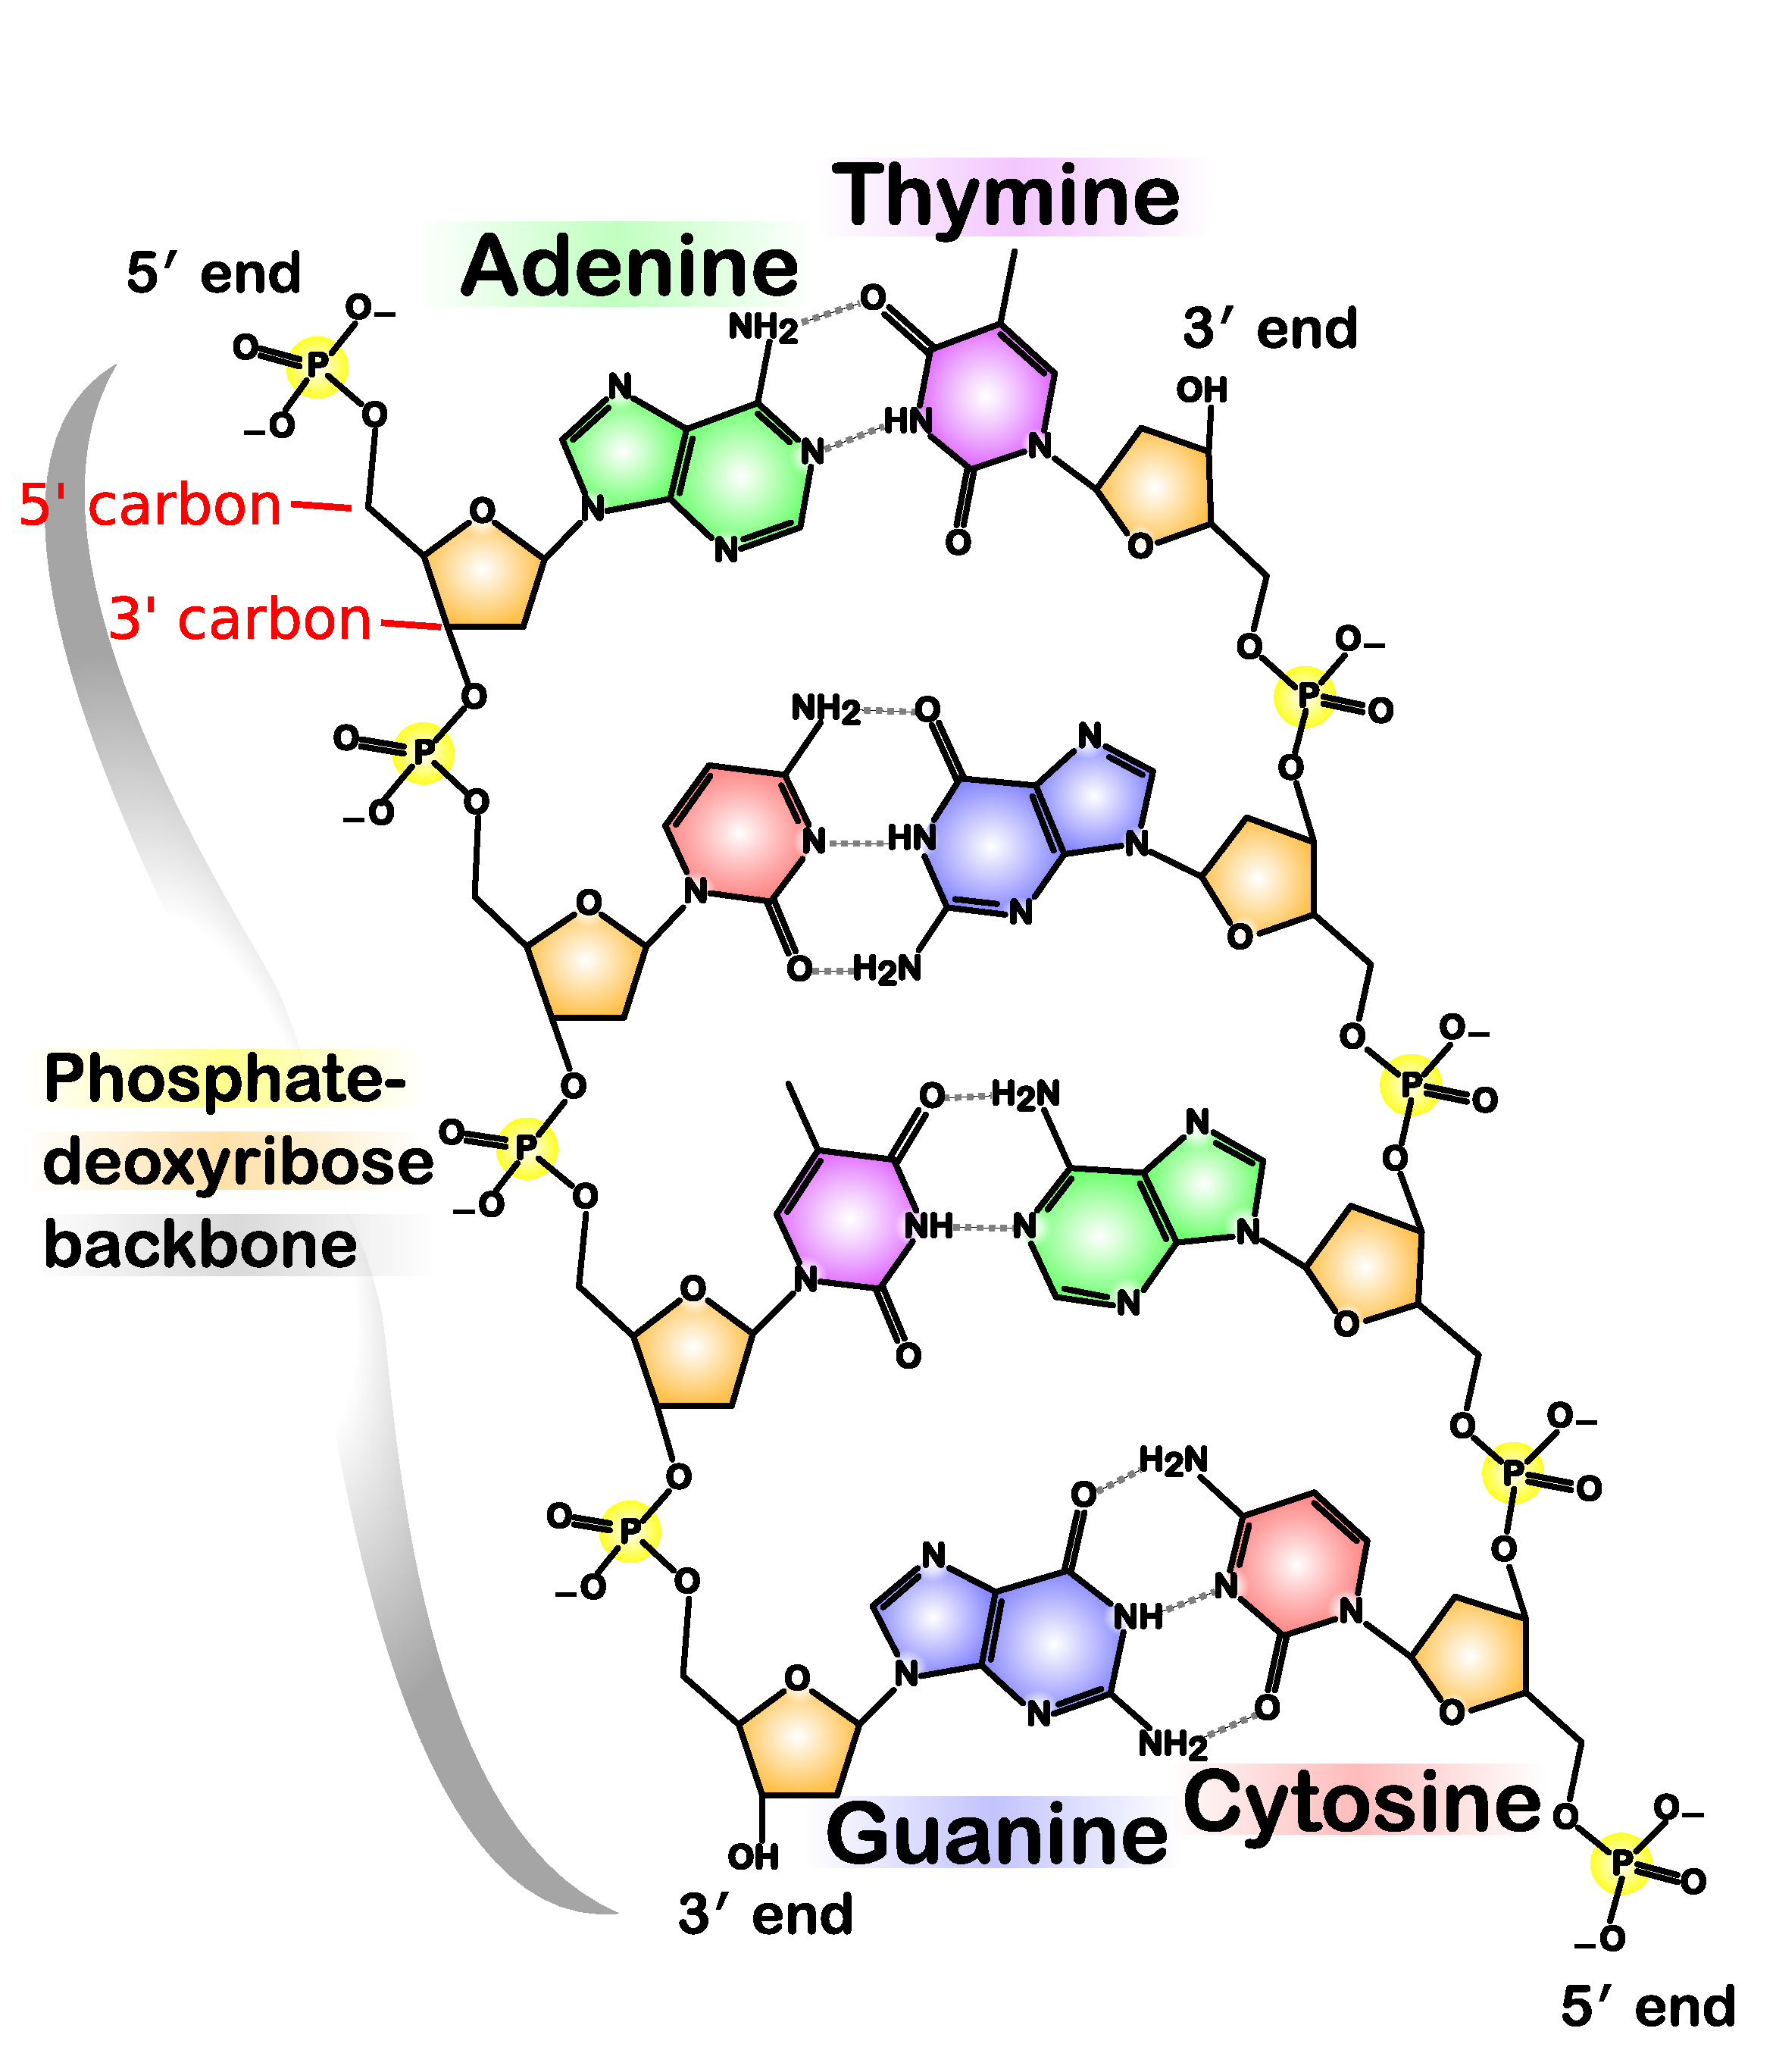
\includegraphics{figs/DNA_chemical_structure} 

}

\caption{Schematic of the structure of DNA. (Figure By Madprime (talk---contribs)  CC BY-SA 3.0, https://commons.wikimedia.org/w/index.php?curid=1848174)}\label{fig:dna-structure}
\end{figure}

The orange parts show the ribose molecules in the backbone, while the four remaining colors
denote the nucleotide bases of adenine (A), cytosine (C), guanine (G), and thymine (T). Each base
on one strand is associated with its \emph{complement} on the other strand. The hydrogen bonds between
complements is what holds the two strands of DNA together. A and T are complements, and
C and G are complements. (I remember this by noting that C and G and curvy and A and T are sharp and
angular, so the pairs go together\ldots{}).

Immediately this raises two challenges that must be resolved for making a simple,
text-based representation of DNA:

\begin{enumerate}
\def\labelenumi{\arabic{enumi}.}
\tightlist
\item
  When describing a sequence of DNA bases, which direction will we read it in?
\item
  Which strand will we read off of?
\end{enumerate}

We leave the second question until later. But note that the order in which DNA sequence
is read is, by convention, from the 5' to the 3' end of the molecule. The terms 3' and 5'
refer to different carbon atoms on the ribose backbone molecules. In the figure above,
each little ``kink'' in the ribose molecule ring (and in the attached lines) is a carbon molecule.
If you count clockwise from the oxygen in ribose, you see that the third carbon (the 3' carbon) is the
carbon atom that leads to a phosphate group, and through the phosphate, to an attachment with the
5' carbon atom of the next ribose. The 3' and 5' carbon atoms are labelled in red
on the top-left ribose molecule in Figure \ref{fig:dna-structure}.

Notice that when we speak of reading a DNA sequence, we are implicitly talking about
reading the sequence of one of the two strands of the double-stranded DNA molecule.
I'll say it again: a DNA sequence is always the sequence of one \emph{strand} of the molecule.
But, if that DNA were ``out living in the wild'' it would have been in double-stranded
form, and would have been paired with its complement sequence. For now, just note
that any DNA sequence always has a complement which is read in the reverse direction.
Thus, if we have a sequence like:

\begin{verbatim}
5'--ACTCGACCT--3'
\end{verbatim}

Then, paired with its complement it would look like:

\begin{verbatim}
5'--ACTCGACCT--3'
    |||||||||
3'--TGAGCTGGA--5'
\end{verbatim}

and, if you were to write its complement in standard 5' to 3' order,
you would have to reverse it like so:

\begin{verbatim}
5'--AGGTCGAGT--3'
\end{verbatim}

\hypertarget{dna-replication-with-dna-polymerase}{%
\subsection{DNA Replication with DNA Polymerase}\label{dna-replication-with-dna-polymerase}}

So, why do we read DNA sequence from 5' to 3'? Is it just because geneticists are wacky, backwards
folks and thought it would be fun to read in a direction that sounds, numerically, to be
backwards? No! It is because \(5'\longrightarrow 3'\) is the direction in
which a new strand of DNA is
synthesized during DNA replication.

When \citet{watsonMolecularStructureNucleic1953} published the first account of the double helical structure of DNA,
they noted that the double-helix (i.e., two-stranded) nature of the molecule immediately suggested
a copying mechanism (Figure \ref{fig:crickwat}).

\begin{figure}

{\centering 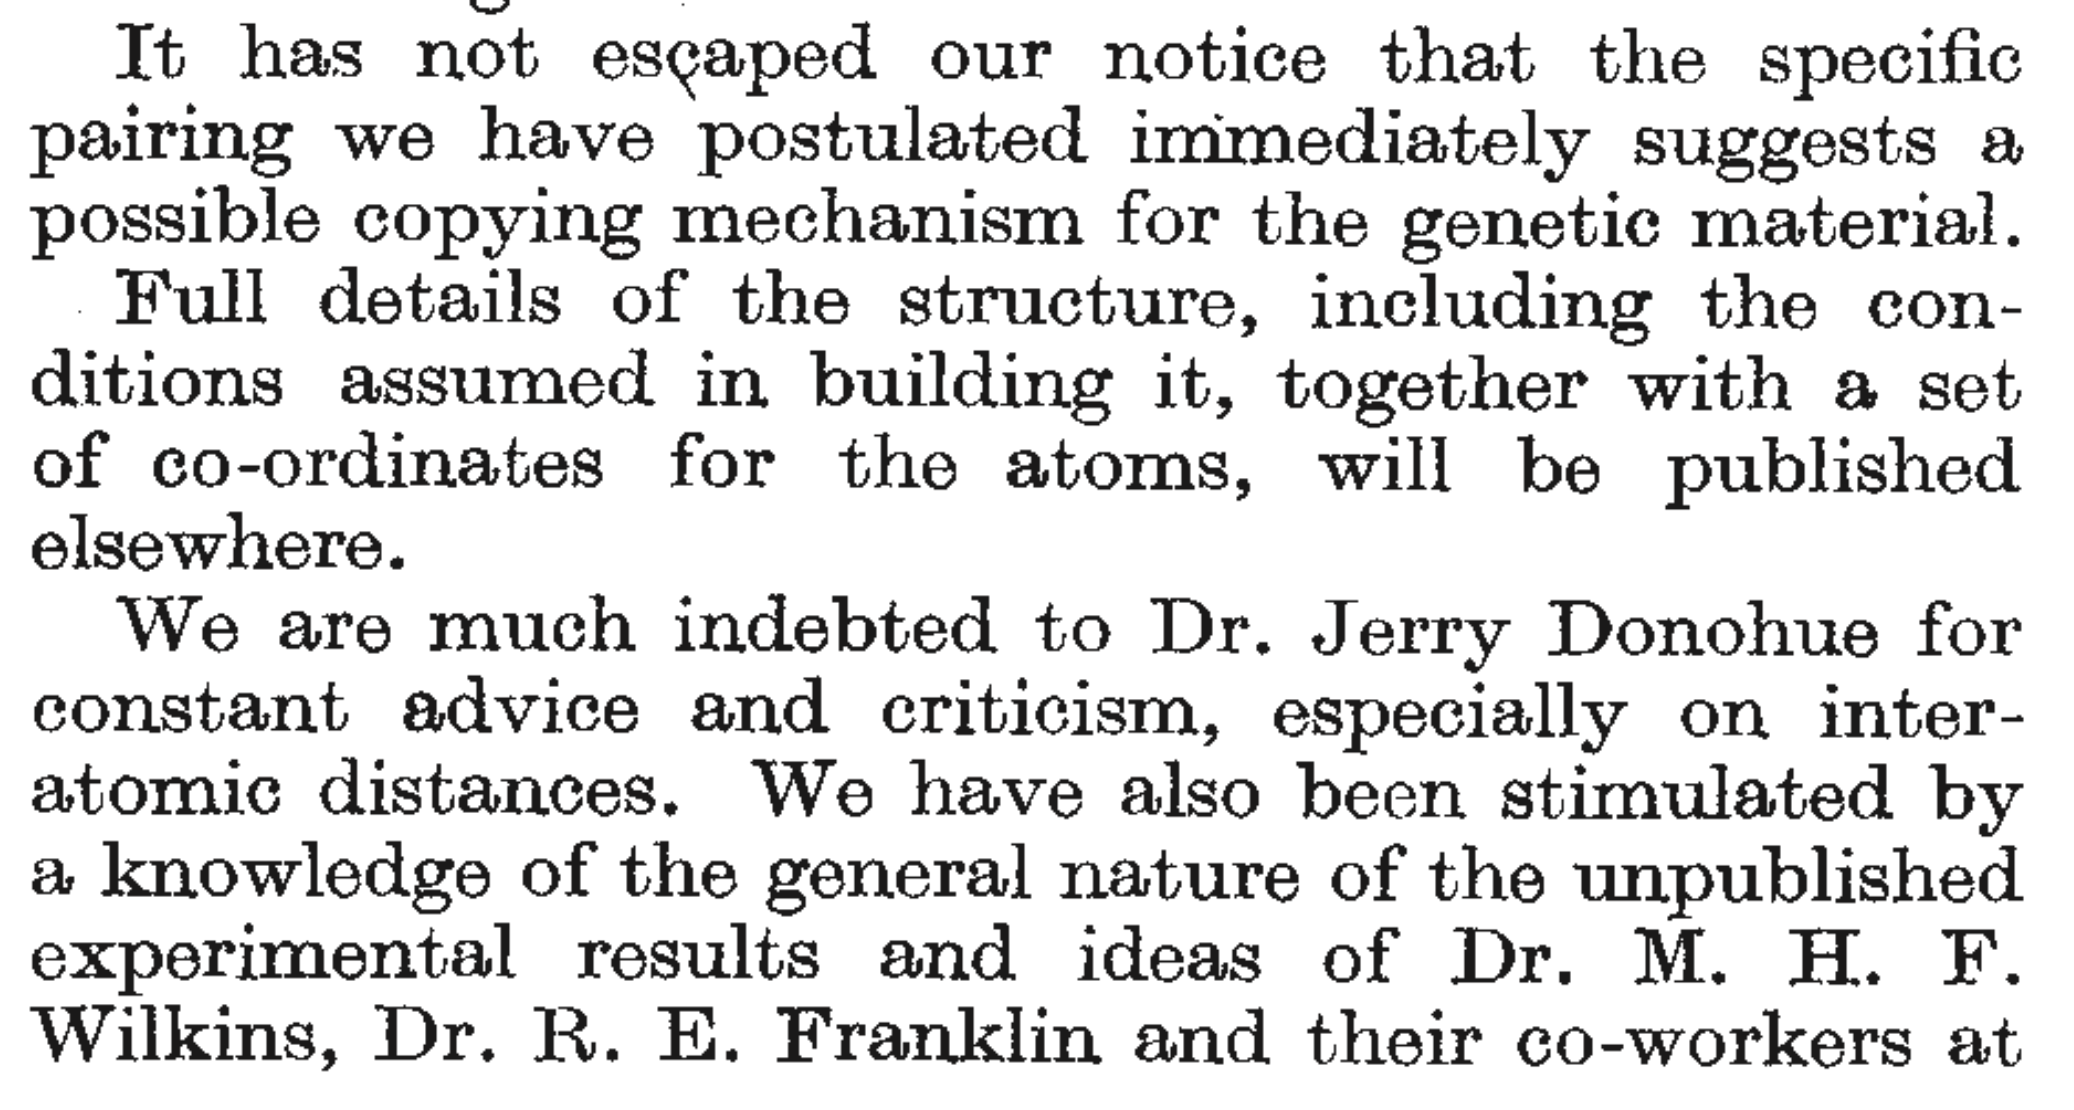
\includegraphics{figs/crick-and-watson} 

}

\caption{Excerpt from Crick and Watson (1953).}\label{fig:crickwat}
\end{figure}

(I've also included, in the excerpt, the inadequate acknowledgment
of the centrality of Rosalind Franklin's pioneering
X-ray crystallography results to Crick and Watson's conclusions---an issue in scientific history about
which much has been written, see, for example, this \href{https://www.theguardian.com/science/2015/jun/23/sexism-in-science-did-watson-and-crick-really-steal-rosalind-franklins-data}{article} in \emph{The Guardian}.)

Figure \ref{fig:dna-copying} shows a schematic of what DNA looks like during the replication process.

\begin{figure}

{\centering 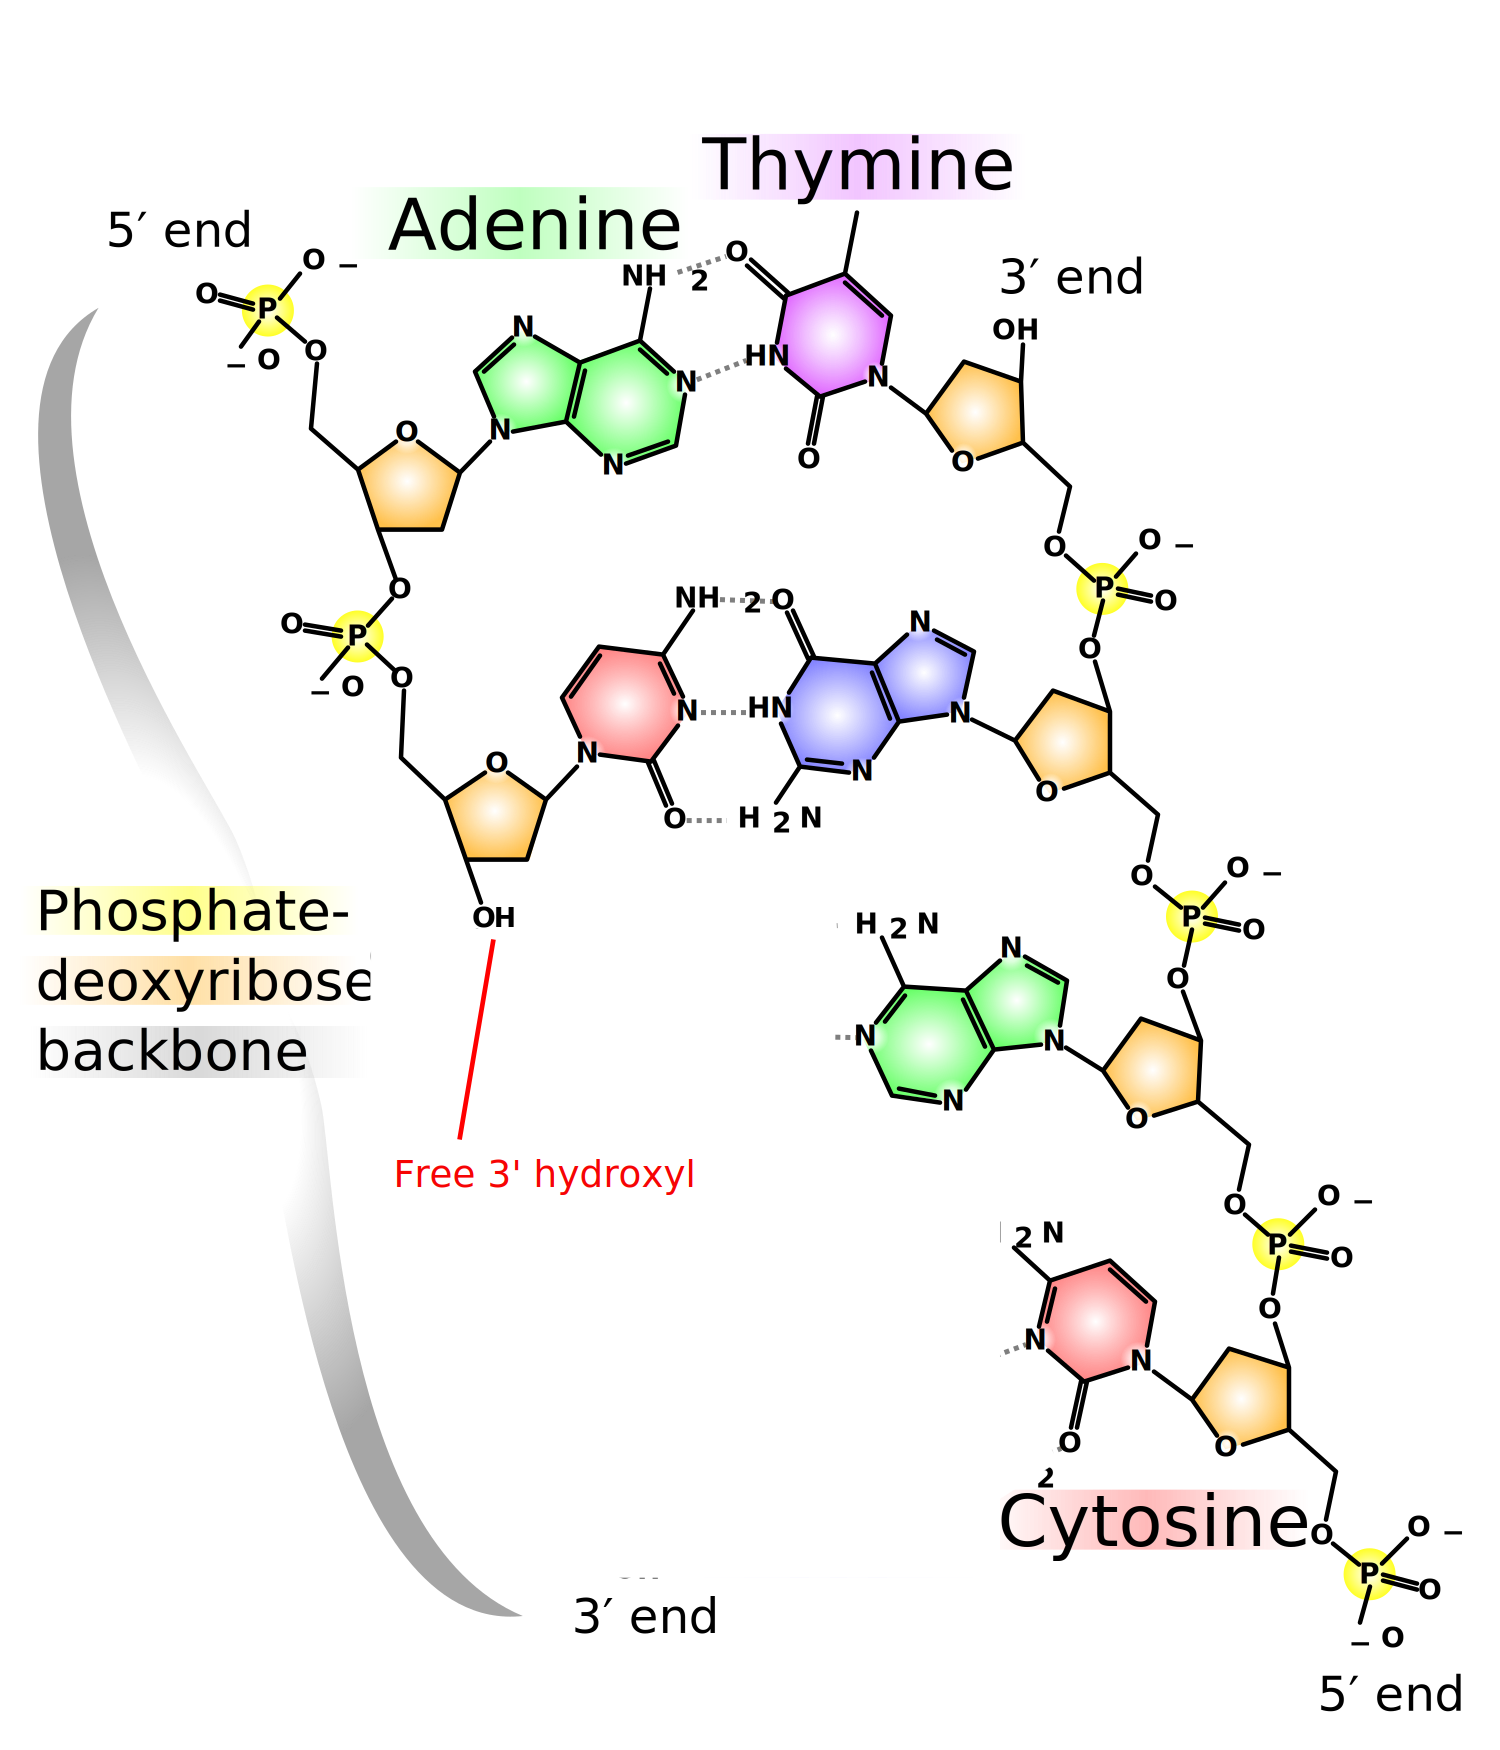
\includegraphics{figs/DNA_chemical_structure_2} 

}

\caption{DNA during replication. (Figure adapted from the one by Madprime (talk---contribs)  CC BY-SA 3.0, https://commons.wikimedia.org/w/index.php?curid=1848174)}\label{fig:dna-copying}
\end{figure}

Essentially, during DNA replication, a \emph{DNA polymerase} molecule finds nucleotide bases (attached
to three phoshpate groups) to build a new strand
that is complementary to the DNA \emph{template} strand, and it guides
those \emph{nucleotide triphosphates} to the appropriate
place in the complementary strand and helps them be incorporated into that growing,
complementary strand. The newly syntesized strand is a
\emph{reverse complement} of the template strand. However, DNA polymerase is not capable of
``setting up shop'' anywhere upon a template strand and simply stuffing complementary bases
in wherever it wants. In fact, DNA polymerase is only able to add new
bases to a growing strand if it can attach the new nucleotide triphosphate to a \emph{free 3' hydroxyl}
that is on the end of the growing strand (the 3' hydroxyl is just a hydroxyl
group attached to the 3' carbon). In Figure \ref{fig:dna-copying}, the template
strand is the strand on the right of the figure, and the growing complementary strand
is on the left side. There is a free 3' hydroxyl group on the ribose attached to the cytosine
base. That is what is needed for DNA polymerase to be able to place a
thymine triphosphate (complementary to adenine on
the template strand) in the currently vacant position. If that thymine comes with a free
3' hydroxyl group, then DNA polymerase will next place a guanine (complementary to the
cytosine on the template strand) on the growing chain. And so forth. Thus, we see
how the new strand of DNA is synthesized from the 5' to the 3' end \emph{of the growing chain}.

Of course, some people find it easier to think about a new strand of DNA being sythesized in
the 3' to 5' direction \emph{along the template strand}. This is equivalent. However, if you just remember
that ``free three'' rhymes, and that DNA polymerase needs a free 3' hydroxyl to add a new base
to the growing strand, you can always deduce that DNA must ``grow'' in a 5' to 3' direction.

\hypertarget{the-importance-of-the-3-hydroxyl}{%
\subsection{The importance of the 3' hydroxyl\ldots{}}\label{the-importance-of-the-3-hydroxyl}}

It would be hard to overstate the importance to molecular biology
of DNA polymerase's dependence upon
a free 3' hydroxyl group for new strand synthesis. This simple fact plays a central
role in:

\begin{enumerate}
\def\labelenumi{\arabic{enumi}.}
\tightlist
\item
  polymerase chain reaction (PCR)---the PCR primers are little oligonucleotides
  that attach to a template strand and provide a free 3' hydroxyl group for the initiation
  of synthesis.
\item
  a ddNTP is a nucleotide attached to a ribose molecule
  that lacks a hydroxyl group on its 3' carbon. Incorporation of
  such a ddNTP into a growing DNA strand terminates further DNA extension, and forms
  the basis for Sanger sequencing (we'll explore this below).
\item
  Some medications are designed to interfere with viral DNA replication. For example,
  AZT, or azino-thymine, is an anti-retroviral drug used to slow the progression of AIDS.
  It is a thymine nucleotide with an azino (\(\mathrm{N}_3\)) group (instead
  of a hydroxyl group) attached to the 3' carbon. Azino-thymine is used preferentially
  by reverse transcriptase when synthesizing DNA. Incorporation of it into a growing
  chain terminates DNA synthesis.
\end{enumerate}

The reversible inhibition of DNA extension also plays an important role in
sequencing by synthesis as used by Illumina platforms. We will discuss
this in a moment, but first we take a stroll down memory lane to refresh our
understanding of \emph{Sanger sequencing} so as to understand how radically different
\emph{next-generation sequencing} technologies are.

\hypertarget{sanger-sequencing}{%
\section{Sanger sequencing}\label{sanger-sequencing}}

It is hard to imagine that the first public human genome was sequenced almost
entirely by Sanger sequencing. We discuss the Sanger sequencing method
here so we can contrast it with what happens on, say, an Illumina machine
today.

To perform Sanger sequencing, first it was necessary to do PCR to
create numerous copies of a double stranded DNA fragment that was to be
sequenced. For example let's say that one wanted to sequence the
20-mer shown below, represented as double stranded DNA.

\begin{verbatim}
5'--AGGCTCAAGCTTCGACCGT--3'
3'--TCCGAGTTCGAAGCTGGCA--5'
\end{verbatim}

For Sanger sequencing, first, one would do PCR to create
bazillions of copies of that double-stranded DNA. Then four separate further PCR
reactions would be done, each one having been ``spiked'' with a little bit of
one of four different ddNTPs which, if incorporated into the
growing strand allow no further extension of it.

For example, if PCR were done as usual, but with the addition of ddATP,
then occasionally, when a ddATP (an A lacking a 3' hydroxyl group)
is incorporated into the growing strand that strand will grow no more.
Consequently, the products of that PCR (incorporating an appropriate
concentration of ddATPs), once filtered to retain only
the top strand from above, will include the fragments

\begin{verbatim}
## [1] "A*"               "AGGCTCA*"        
## [3] "AGGCTCAA*"        "AGGCTCAAGCTTCGA*"
\end{verbatim}

Where the \texttt{*} follows the sequence-terminating base.

Likewise, in a separate reaction, occasional incorporation of a ddCTP will yield products:

\begin{verbatim}
## [1] "AGGC*"              "AGGCTC*"           
## [3] "AGGCTCAAGC*"        "AGGCTCAAGCTTC*"    
## [5] "AGGCTCAAGCTTCGAC*"  "AGGCTCAAGCTTCGACC*"
\end{verbatim}

And in another reaction, occasional incorporation of ddGTP yields:

\begin{verbatim}
## [1] "AG*"                 "AGG*"               
## [3] "AGGCTCAAG*"          "AGGCTCAAGCTTCG*"    
## [5] "AGGCTCAAGCTTCGACCG*"
\end{verbatim}

And in a final, separate reaction, incorporation of ddTTP would give:

\begin{verbatim}
## [1] "AGGCT*"               "AGGCTCAAGCT*"        
## [3] "AGGCTCAAGCTT*"        "AGGCTCAAGCTTCGACCGT*"
\end{verbatim}

Each of these fragments is of a different length, so they can be
separated on an electrophoretic gel. The secret to Sanger sequencing is that
the products of all four separate reactions can be run side by side in
separate lanes of the gel (or, as was done later, in separate capillaries\ldots{}),
so that the gel, with small
fragments running faster than large fragments, from the top to the bottom
of the gel, would look like Figure \ref{fig:sanger}:
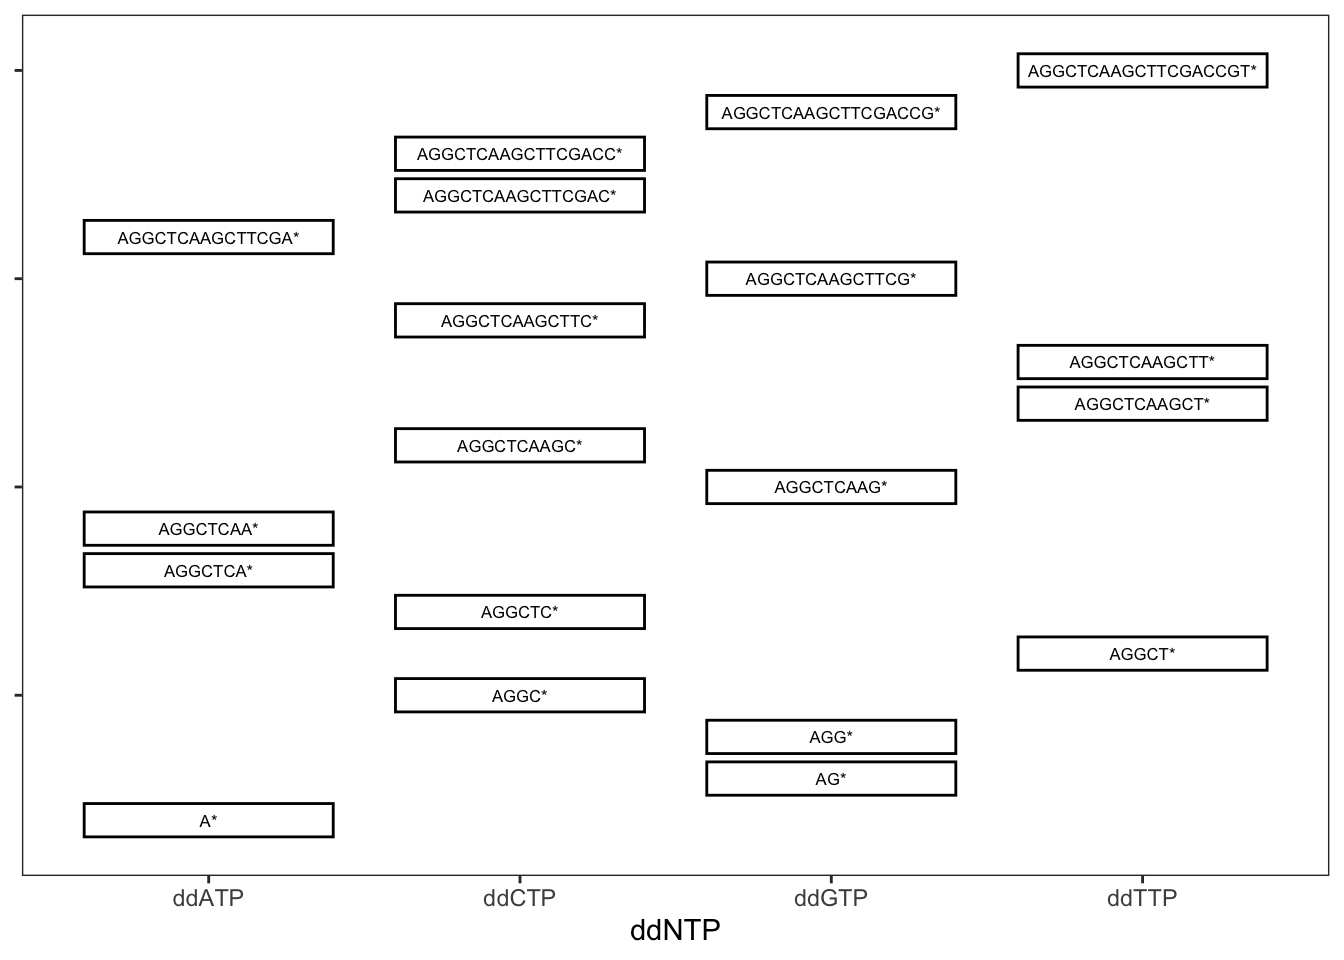
\includegraphics{eca-bioinf-handbook_files/figure-latex/sanger-1.pdf}

In reality, a gel like that in Figure \ref{fig:sanger}, won't bear the name of each
sequence fragment. In fact, it will look much more like what you see in Figure \ref{fig:sanger2}.
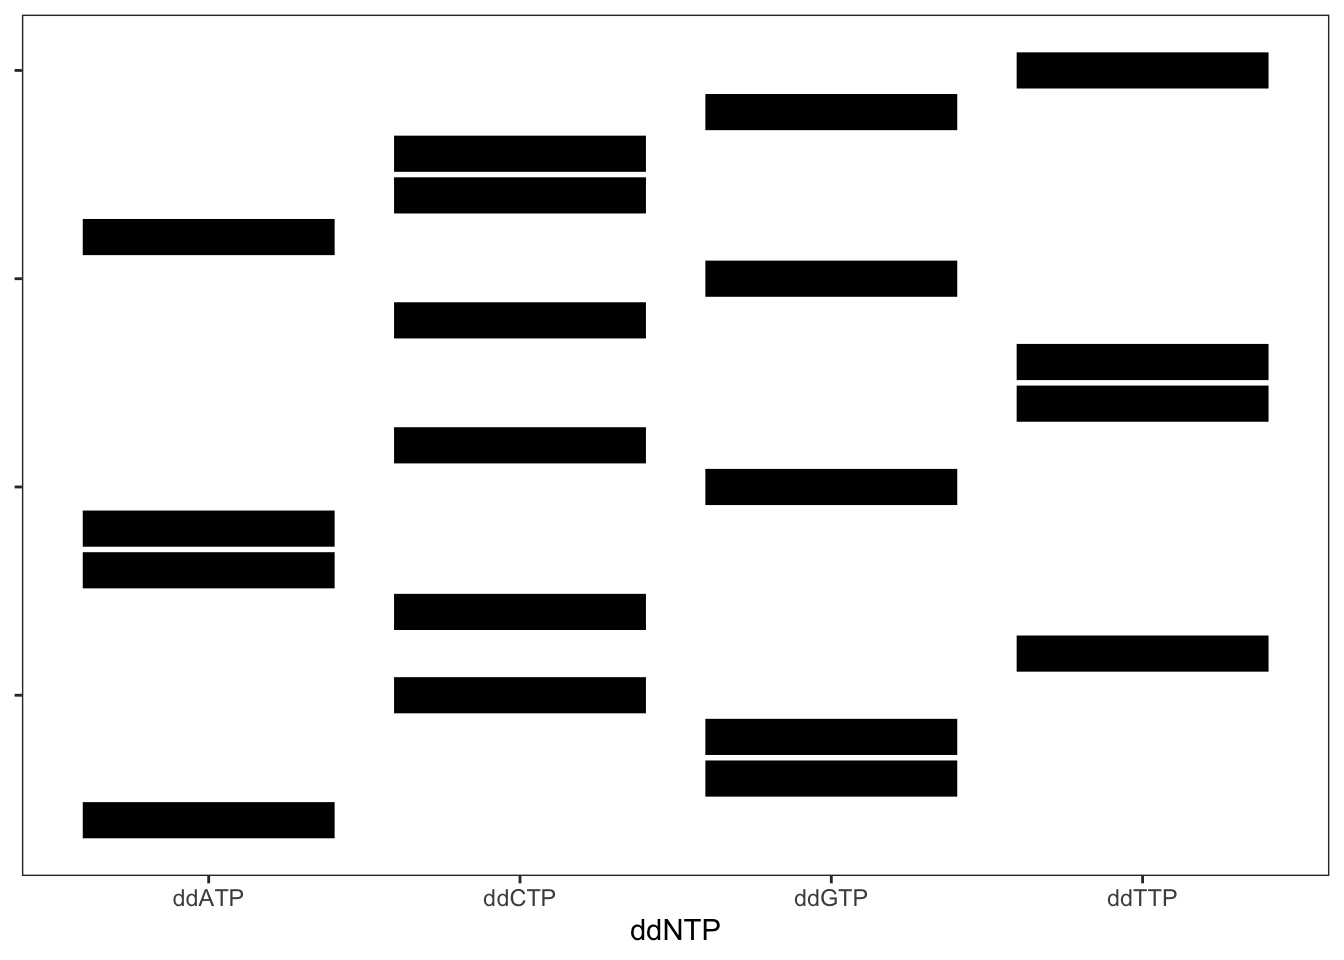
\includegraphics{eca-bioinf-handbook_files/figure-latex/sanger2-1.pdf}
However, even with the DNA fragemnt sequences obscured, their sequences can be
detemined by working from the bottom to the top and adding a different DNA base according to which column the band is in. Try it out.

Some very important points must be made about Sanger sequencing:

\begin{enumerate}
\def\labelenumi{\arabic{enumi}.}
\tightlist
\item
  The signal obtained from sequencing is, in a sense, a mixture of the starting templates. So, if you
  have DNA from an individual, you have two copies of each chromosome, and they might carry slightly
  different sequences. At heterozygous sites, it is impossible to tell which allele came from which
  chromosome.
\item
  To conduct this procedure, it was typical that specific PCR primers were used to sequence
  only a single fragment of interest. Extending the sequencing beyond that region often involved
  a laborious process of ``walking'' primers further out in either direction. Very tedious.
\item
  Each sequencing reaction was typically carried out for just a single individual at once.\\
\item
  Until a little over a decade ago, this is how sequencing was done in conservation genetics.
\end{enumerate}

\hypertarget{illumina-sequencing-by-synthesis}{%
\section{Illumina Sequencing by Synthesis}\label{illumina-sequencing-by-synthesis}}

Illumina paired-end sequencing is currently the leading technology in conservation
genomics.

They say that a picture is worth a thousand words, so a video may well be worth
ten thousand. Illumina has a very informative video about sequencing by synthesis.

I have used some code (I found on GitHub) to provide captions to the video. These captions
include comments, as well as questions that form part of this week's homework. (Yay!)\\
You can see the video at
\url{https://eriqande.github.io/erics-captioned-vids/vids/illumina-sbs/}

The main take-home messages I want everyone to get about Illumin sequencing is:

\begin{enumerate}
\def\labelenumi{\arabic{enumi}.}
\tightlist
\item
  The signal obtained from each cluster is the sequence of a single, \emph{single-stranded DNA fragment}
\item
  In paired-end sequencing, sequence from both ends of the fragment (but not necessarily
  the middle) is obtained.
\item
  The technique lends itself to sequencing millions of ``anonymous'' chunks of DNA.
\item
  The indexes, or ``barcodes'' allow DNA from multiple individuals to be sequenced in a single run.
\item
  This is how most high-throughput sequencing is done today.
\end{enumerate}

\hypertarget{library-prep-protocols}{%
\section{Library Prep Protocols}\label{library-prep-protocols}}

Gotta mention here about how barcodes work.

How you prepare your libraries dictates what type of data you get.

\hypertarget{wgs}{%
\subsection{WGS}\label{wgs}}

\hypertarget{rad-seq-methods}{%
\subsection{RAD-Seq methods}\label{rad-seq-methods}}

\hypertarget{amplicon-sequencing}{%
\subsection{Amplicon Sequencing}\label{amplicon-sequencing}}

\hypertarget{capture-arrays-rapture-etc.}{%
\subsection{Capture arrays, RAPTURE, etc.}\label{capture-arrays-rapture-etc.}}

\hypertarget{bioinformatic-file-formats}{%
\chapter{Bioinformatic file formats}\label{bioinformatic-file-formats}}

Almost all the high-throughput sequencing data you will deal with should
arrive in just a few different formats. There are some specialized formats
(like those output by the program TASSEL, etc.) but we will largely ignore
those, focusing instead on the formats used in production by the 1000 genomes
and 10K vertebrate genomes projects. In a sentence, the most important are:
FASTA, FASTQ, SAM, BAM, and VCF.

Plan: Go over these, and for each, pay special attention to compressed and indexed
forms and explain why that is so important. I think that we should probably
talk about the programs that are available for manipulating each of these, as well,
but I won't add that until we all have access to an HPC or other proper
Unix environment.

I was originally going to do tools for manipulating files in the different
formats, but I will do that in a separate chapter(s) later.

\hypertarget{sequences}{%
\section{Sequences}\label{sequences}}

\hypertarget{fastq}{%
\section{FASTQ}\label{fastq}}

The FASTQ format is the standard format for lightly-processed data
coming off an Illumina machine. If you are doing whole genome sequencing,
it is typical for the Illumina processing pipeline to have separated all
the reads with different barcodes into different, separate files. Typically
this means that all the reads from one library prep for one sample will
be in a single file. The barcodes and any associated additional adapter
sequence is typically also removed from the reads. If you are processing
RAD data, the reads may not be separated by barcode, because, due to the
vagaries of the RAD library prep, the barcodes might appear on different ends
of some reads than expected.

A typical file extension for FASTQ files is \texttt{.fq}.
Almost all FASTQ files you get from a sequencer should be gzipped to save space.
Thus, in order to view the file you will have to uncompress it. Since you would,
in most circumstances, want to visually inspect just a few lines, it is best
to do that with \texttt{gzcat} and pipe the output to \texttt{head}.

As we have seen, paired-end sequencing produces two separate reads of a DNA
fragment. Those two different reads are usually stored in two separate files named
in such a manner as to transparently denote whether it contains sequences obtained
from read 1 or read 2.
For example \texttt{bird\_08\_B03\_R1.fq.gz} and \texttt{bird\_08\_B03\_R2.fq.gz}. Read 1 and Read 2 from
a paired read must occupy the sames lines in their respective files, i.e., lines
10001-10004 in \texttt{bird\_08\_B03\_R1.fq.gz} and lines 10001-10004 in \texttt{bird\_08\_B03\_R2.fq.gz}
should both pertain to the same DNA fragment that was sequenced. That is what is
meant by ``paired-end'' sequencing: the sequences come in pairs from different
ends of the same fragment.

The FASTQ format is \emph{very} simple: information about each read occupies just four lines.
This means that the number of lines in a proper FASTQ file must always be a multiple of four.
Briefly, the four lines of information about each read are always in the same order as follows:

\begin{enumerate}
\def\labelenumi{\arabic{enumi}.}
\tightlist
\item
  An Identifier line
\item
  The DNA sequence as A's, C's, G's and T's.
\item
  A line that is almost always simply a \texttt{+} sign, but can optionally be followed
  by a repeat of the ID line.
\item
  An ASCII-encoded, Phred-scaled base quality score. This gives an estimated
  measure of certainty about each base call in the sequence.
\end{enumerate}

The code block below shows three reads worth (twelve lines) of
information from a FASTQ file.
Take a moment to identify the four different lines for each read.

\begin{verbatim}
@K00364:64:HTYYCBBXX:1:1108:4635:14133/1
TAGAATACGCCAGGTGTAAGAATAGTAGAATACGCCAGGTGTAAGAATAGTAGAACACGCCAGGTGTAAGAATAGTAGAA
+
AAAFFJJJJJFFJFJJJFJJFFJFJFJJJJJJJJFFJJJFJJJFJJAJJFJJFJJFJJJ7JJJF-<JAFJJ<F<AJAJJF
@K00364:64:HTYYCBBXX:1:1108:5081:25527/1
AAAACACCAAAAGAAAGATGCCCAGGGTCCCTGCTCATCTGCGTGAAAGTGACTTAGGCATGCTGCAAGGAGGCATGAGG
+
AAFFFJJJJJJJJJJJJJJJJJJJJJJJJJJJJJJJJJJJJJJJJJJJJJJJJJJJJJJJJJJJJJJJJJJJJJJJJJJJ
@K00364:64:HTYYCBBXX:1:1108:5852:47295/1
AGGTGGCTCTAGAAGGTTCTCGGACCGAGAAACAGCCTCGTACATTTGCAATGATTTCAATTCATTTTGACCATTACGAA
+
AAFFFJJJJJJJJJJJJJJJJJJJJJJJJJJJJJJJJJJJJJJJJJJJJJJJJJJJJJJJJJJJJJJJJJJJJJJJJJJJ
\end{verbatim}

Lines 2 and 3 are self-explanatory, but we will expound upon lines 1 and 4 below.

\hypertarget{illumina-ids}{%
\subsection{Line 1: Illumina identifier lines}\label{illumina-ids}}

The identifier line can be just about any string that starts with an \texttt{@}, but, from Illumina data, today,
you will typically see something like this:

\begin{verbatim}
@K00364:64:HTYYCBBXX:1:1108:4635:14133/1
\end{verbatim}

The colons (and the \texttt{/}) are field separators. The separate parts of the line
above are interpreted something along the lines as follows (keeping in mind that
Illumina occasionally changes the format and that there may be additional
optional fields):

\begin{verbatim}
@           : mandatory character that starts the ID line
K00364      : Unique sequencing machine ID 
64          : Run number on instrument
HTYYCBBXX   : Unique flow cell identifier
1           : Lane number
1108        : Tile number (section of the lane)
4635        : x-coordinate of the cluster within the tile
14133       : y-coordinate of the cluster within the tile
1           : Whether the sequence is from read 1 or read 2 
\end{verbatim}

Question: For paired reads, do you expect the x- and y-coordinates for read 1 and read 2 to
be the same?

\hypertarget{line-4-base-quality-scores}{%
\subsection{Line 4: Base quality scores}\label{line-4-base-quality-scores}}

The base quality scores give an estimate of the probability that the base call is incorrect.
This comes from data the sequencer collects on the brightness and compactness of the cluster
radiance, other factors, and Illumina's own models for base call accuracy. If we let \(p\)
be the probability that a base is called incorrectly, then \(Q\), the Phred-scaled base quality
score, is:

\[
Q = \lfloor-10\log_{10}p\rfloor,
\]
where \(\lfloor x \rfloor\) means "the largest integer smaller than \(x\).

To get the estimate of the probability that the base is called incorrectly from
the Phred scaled score, you invert the above equation:

\[
p = \frac{1}{10^{Q/10}}
\]
Base quality scores from Illumina range from 0 to 40.
The easiest values to use as guideposts are \(Q = 0, 10, 20, 30, 40\), which correspond to
error probabilites of 1, 1 in 10, 1 in 100, 1 in 1,000, and 1 in 10,000, respectively.

All this is fine and well, but when we look at the quality score line above we see
something like \texttt{7JJJF-\textless{}JAFJJ\textless{}F\textless{}AJAJJF}. What gives? Well, from a file storage and
parsing perspective, it makes sense to only use a single character to store the
quality score for every base. So, that is what has been done: each of those
single characters represents a quality score---a number between 0 and 40, inclusive.

The values that have been used are the \emph{decimal representations of ASCII text characters} minus 33.\\
The decimal representation or each character can be found in Figure \ref{fig:ascii}.

\begin{figure}

{\centering 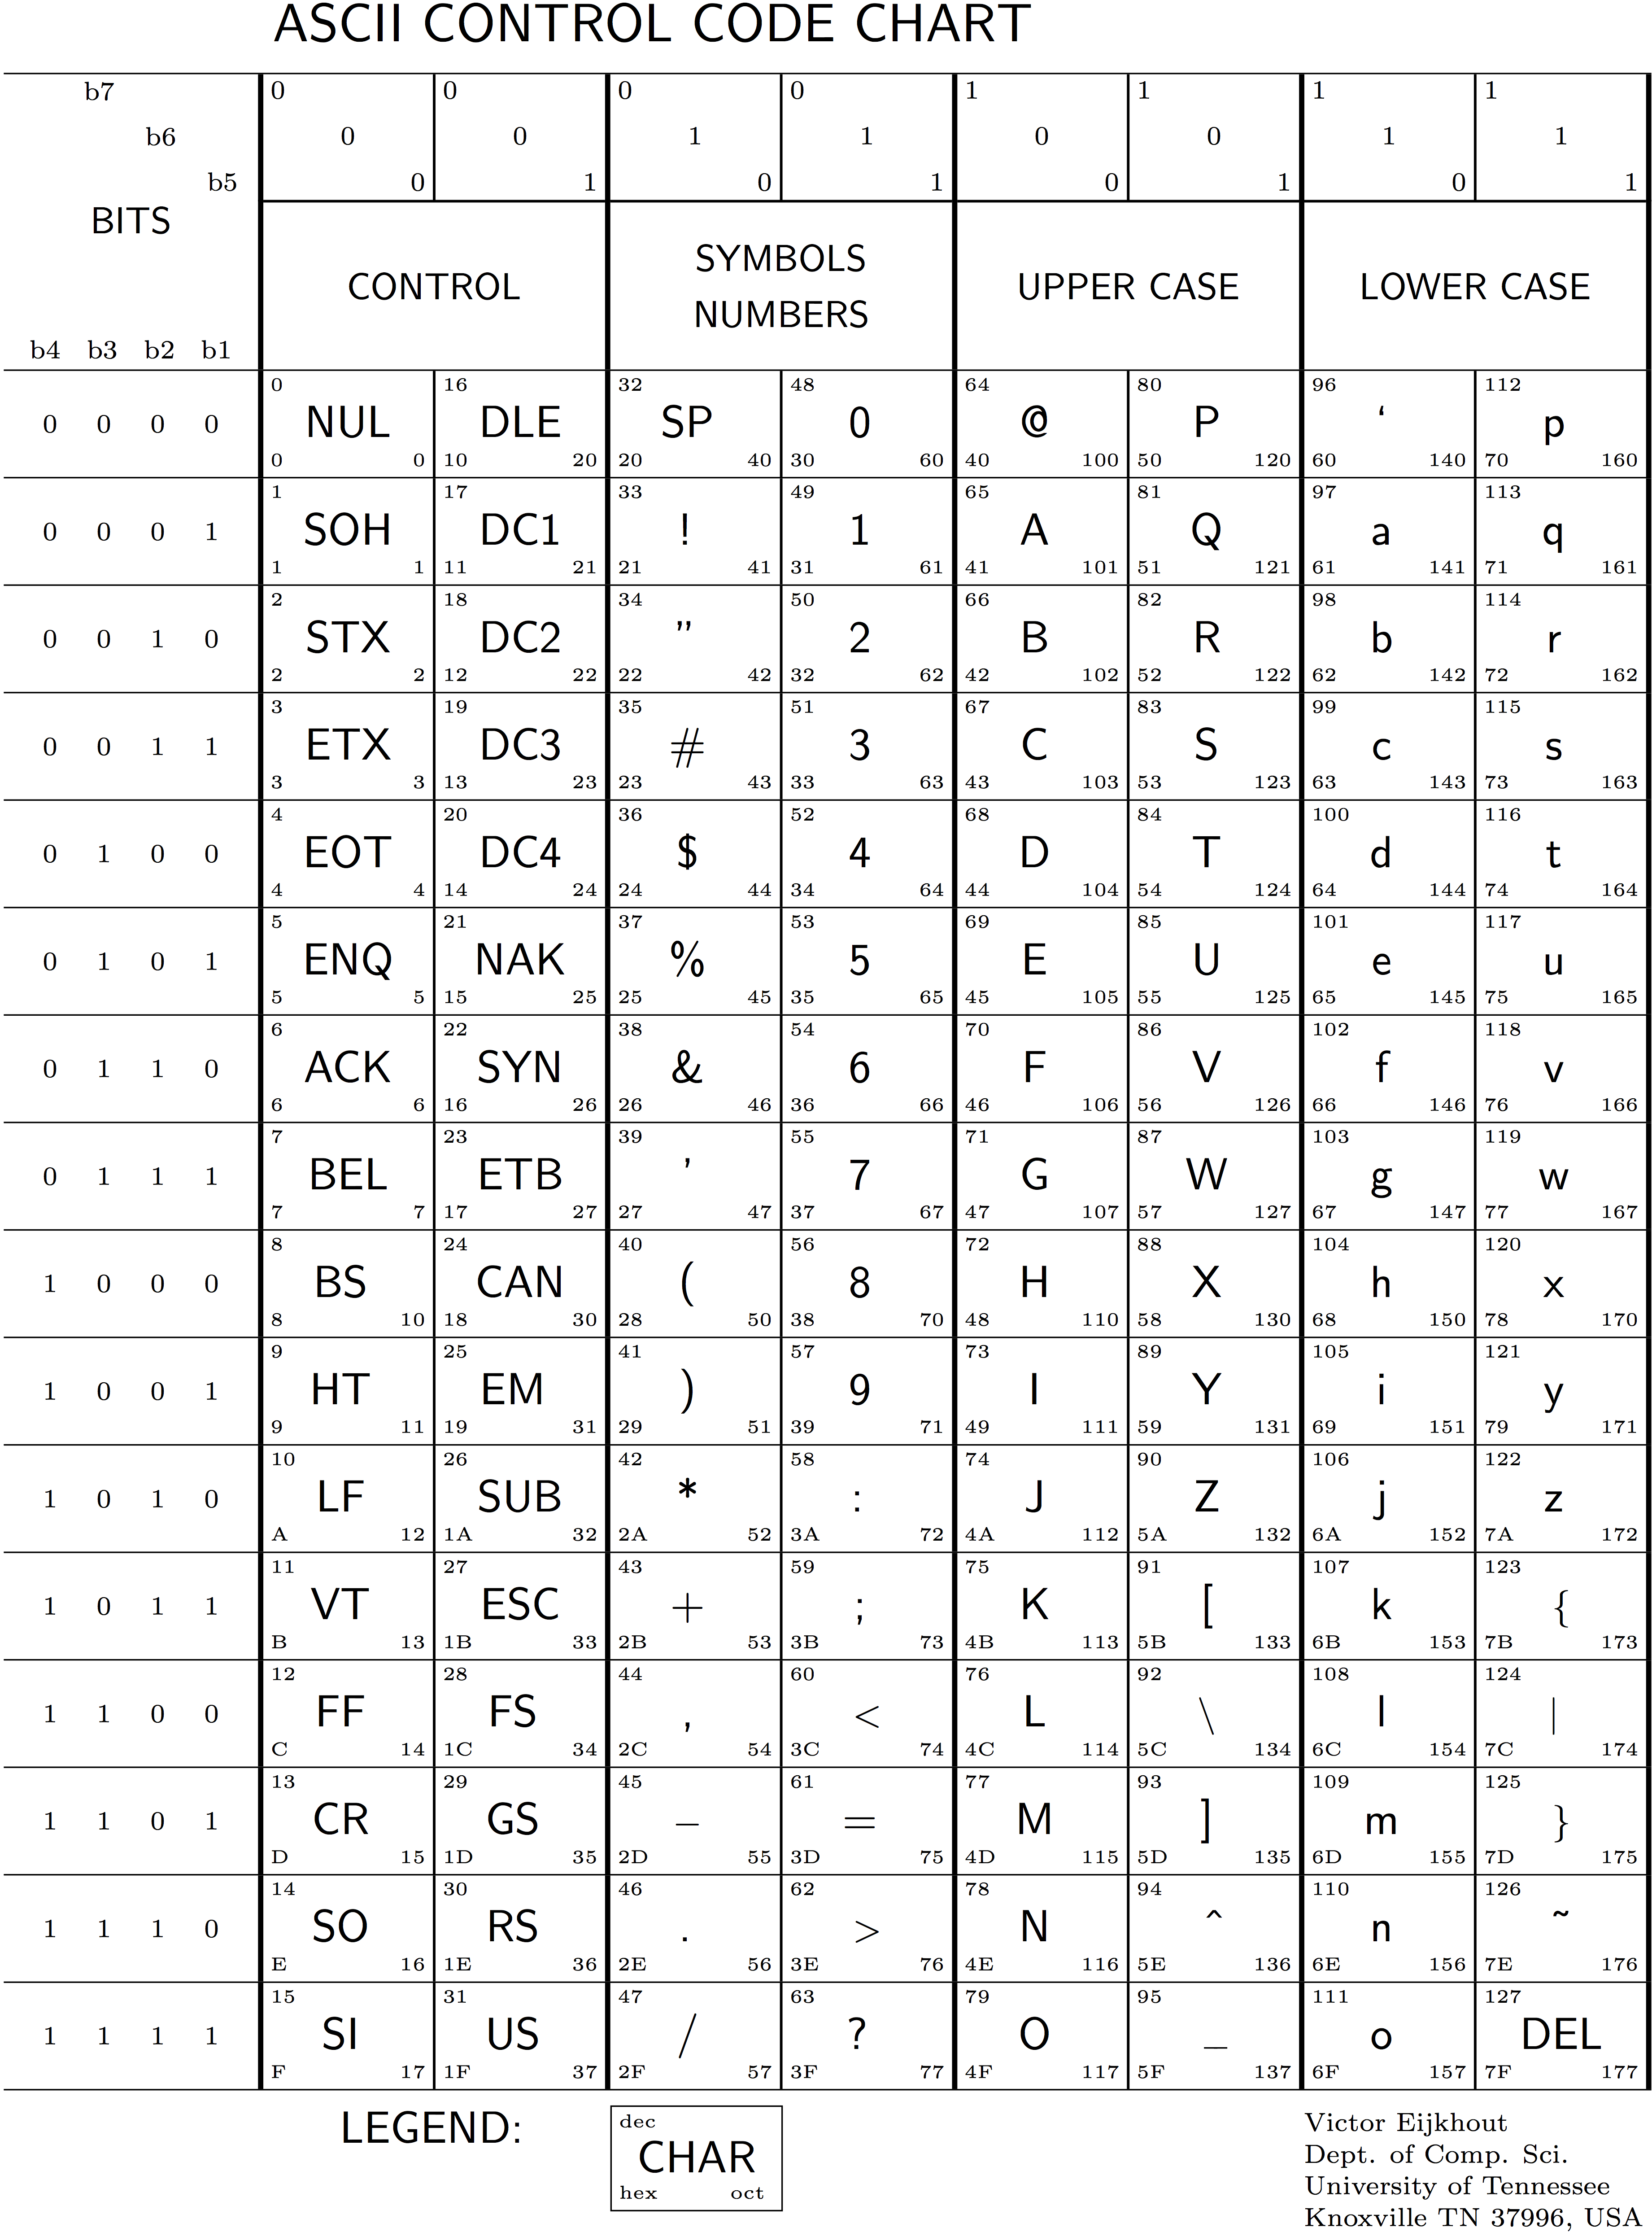
\includegraphics{figs/ascii-crop} 

}

\caption{This lovely ASCII table shows the binary, hexadecimal, octal and decimal representations of ASCII characters (in the corners of each square; see the legend rectangle at bottom.  Table produced from TeX code written and developed by Victor Eijkhout available at [https://ctan.math.illinois.edu/info/ascii-chart/ascii.tex](https://ctan.math.illinois.edu/info/ascii-chart/ascii.tex)}\label{fig:ascii}
\end{figure}

The decimal representation is in the upper left of each character's rectangle.

Find the characters corresponding to base quality scores of 0, 10, 20, 30, and 40. Remember that the
base quality score is the character's decimal representation \emph{minus 33}.

Here is another question: why do you think the scale starts with ASCII character 33?

\hypertarget{a-fastq-tidyverse-interlude}{%
\subsection{A FASTQ `tidyverse' Interlude}\label{a-fastq-tidyverse-interlude}}

Here we demonstrate some R code while exploring FASTQ files. First, in order to
do these exercises you will want to download and launch the RStudio project,
\texttt{big-fastq-play},
that has the data
in it. Please work within that RStudio project to do these exercises.
Here is a direct download link to it:
\url{https://docs.google.com/uc?export=download\&id=1iD8tz_KSOHDBpXvXssqo3noPZAm1Qsjp}

Note that this might stress out older laptops as it loads 100s of Mb of sequence
data into memory.

\hypertarget{reading-fastqs-with-read_lines}{%
\subsubsection{\texorpdfstring{Reading FASTQs with \texttt{read\_lines}}{Reading FASTQs with read\_lines}}\label{reading-fastqs-with-read_lines}}

Load packages:

\begin{Shaded}
\begin{Highlighting}[]
\KeywordTok{library}\NormalTok{(tidyverse)}

\CommentTok{# if you don't have this package, get it}
\CommentTok{# install.packages("viridis")}
\KeywordTok{library}\NormalTok{(viridis)}
\end{Highlighting}
\end{Shaded}

Read the FASTQ, make it a matrix, then make it a tibble

\begin{Shaded}
\begin{Highlighting}[]
\CommentTok{# use read_lines to read the R1 fastq file line by line;}
\CommentTok{# then make a 4 column matrix, filling by rows}
\CommentTok{# then drop column 3, which corresponds to the "+" line}
\NormalTok{R1 <-}\StringTok{ }\KeywordTok{read_lines}\NormalTok{(}\StringTok{"data/Battle_Creek_01_chinook_R1.fq.gz"}\NormalTok{) }\OperatorTok
\StringTok{  }\KeywordTok{matrix}\NormalTok{(}\DataTypeTok{ncol =} \DecValTok{4}\NormalTok{, }\DataTypeTok{byrow =} \OtherTok{TRUE}\NormalTok{) }\OperatorTok
\StringTok{  }\NormalTok{.[,}\OperatorTok{-}\DecValTok{3}\NormalTok{]}
  

\CommentTok{# add colnames}
\KeywordTok{colnames}\NormalTok{(R1) <-}\StringTok{ }\KeywordTok{c}\NormalTok{(}\StringTok{"ID"}\NormalTok{, }\StringTok{"seq"}\NormalTok{, }\StringTok{"qual"}\NormalTok{)}

\CommentTok{# now make a tibble out that.  We will assign}
\CommentTok{# it back to the variable R1, to note carry}
\CommentTok{# extra memory around}
\NormalTok{R1 <-}\StringTok{ }\KeywordTok{as_tibble}\NormalTok{(R1)}

\CommentTok{# Look at it:}
\NormalTok{R1}


\CommentTok{# OK, 1 million reads.}
\end{Highlighting}
\end{Shaded}

Look at the first ID line:

\begin{verbatim}
 @E00430:101:HKT7WCCXY:1:1101:6411:1204 1:N:0:NGATGT
\end{verbatim}

Aha! This is a slightly different format than the above. The part after the
space has colon-separated fields that are:

\begin{verbatim}
1        :  which read of the pair
N        :  has this been filtered (Y/N)
0        :  control number (always 0 on HiSeq and NextSeq)
NGATGT   :  barcode on the read
\end{verbatim}

OK, our mission is to actually look at the locations of these reads on different
tiles. To do that we will want to access the x and y coordinates and the
tiles, etc. In the tidyverse, this means giving each of those things its own
column.

\hypertarget{tidyrseparate}{%
\subsubsection{tidyr::separate()}\label{tidyrseparate}}

How do we break those colon-separated fields into columns? This is a job for
\texttt{tidyr::separate} which breaks a text string on user-defined separators into
columns in a tibble.

Here we can use it to break the ID into two parts split on the space, and then
break the first part of the ID into its constituent parts:

\begin{Shaded}
\begin{Highlighting}[]
\CommentTok{# first we break on the space,}
\CommentTok{# then we break the ID on the colons, but keep the original "id" for later}
\NormalTok{R1 }\OperatorTok
\StringTok{  }\KeywordTok{separate}\NormalTok{(ID, }\DataTypeTok{into =} \KeywordTok{c}\NormalTok{(}\StringTok{"id"}\NormalTok{, }\StringTok{"part2"}\NormalTok{), }\DataTypeTok{sep =} \StringTok{" "}\NormalTok{) }\OperatorTok
\StringTok{  }\KeywordTok{separate}\NormalTok{(}
\NormalTok{    id, }
    \DataTypeTok{into =} \KeywordTok{c}\NormalTok{(}\StringTok{"machine"}\NormalTok{, }\StringTok{"run"}\NormalTok{, }\StringTok{"flow_cell"}\NormalTok{, }\StringTok{"lane"}\NormalTok{, }\StringTok{"tile"}\NormalTok{, }\StringTok{"x"}\NormalTok{, }\StringTok{"y"}\NormalTok{), }
    \DataTypeTok{sep =} \StringTok{":"}\NormalTok{,}
    \DataTypeTok{remove =} \OtherTok{FALSE}
\NormalTok{    )}
\end{Highlighting}
\end{Shaded}

Wow! That was cool. Now, your mission is to pipe that (with \texttt{\%\textgreater{}\%})
into another \texttt{separate()} command that breaks part2 into
\texttt{read}, \texttt{filter}, \texttt{cnum}, and \texttt{barcode}, and save that into \texttt{R1\_sep}

Here is a starter:

\begin{Shaded}
\begin{Highlighting}[]
\NormalTok{R1_sep <-}\StringTok{ }\NormalTok{R1 }\OperatorTok
\StringTok{  }\KeywordTok{separate}\NormalTok{(ID, }\DataTypeTok{into =} \KeywordTok{c}\NormalTok{(}\StringTok{"id"}\NormalTok{, }\StringTok{"part2"}\NormalTok{), }\DataTypeTok{sep =} \StringTok{" "}\NormalTok{) }\OperatorTok
\StringTok{  }\KeywordTok{separate}\NormalTok{(}
\NormalTok{    id, }
    \DataTypeTok{into =} \KeywordTok{c}\NormalTok{(}\StringTok{"machine"}\NormalTok{, }\StringTok{"run"}\NormalTok{, }\StringTok{"flow_cell"}\NormalTok{, }\StringTok{"lane"}\NormalTok{, }\StringTok{"tile"}\NormalTok{, }\StringTok{"x"}\NormalTok{, }\StringTok{"y"}\NormalTok{), }
    \DataTypeTok{sep =} \StringTok{":"}\NormalTok{,}
    \DataTypeTok{remove =} \OtherTok{FALSE}
\NormalTok{    ) }\OperatorTok
\StringTok{    }\NormalTok{...your code here...}
    
\CommentTok{# when you are done with that, look at it}
\NormalTok{R1_sep}
    
\end{Highlighting}
\end{Shaded}

Doh! There is one thing to note. Look at the first few columns of that:

\begin{Shaded}
\begin{Highlighting}[]
\CommentTok{# A tibble: 1,000,000 x 11}
\NormalTok{   id          machine run   flow_cell lane  tile  x     y   }
   \OperatorTok{<}\NormalTok{chr}\OperatorTok{>}\StringTok{       }\ErrorTok{<}\NormalTok{chr}\OperatorTok{>}\StringTok{   }\ErrorTok{<}\NormalTok{chr}\OperatorTok{>}\StringTok{ }\ErrorTok{<}\NormalTok{chr}\OperatorTok{>}\StringTok{     }\ErrorTok{<}\NormalTok{chr}\OperatorTok{>}\StringTok{ }\ErrorTok{<}\NormalTok{chr}\OperatorTok{>}\StringTok{ }\ErrorTok{<}\NormalTok{chr}\OperatorTok{>}\StringTok{ }\ErrorTok{<}\NormalTok{chr}\OperatorTok{>}\StringTok{      }
\StringTok{ }\DecValTok{1} \OperatorTok{@}\NormalTok{E00430}\OperatorTok{:}\NormalTok{10… }\OperatorTok{@}\NormalTok{E00430 }\DecValTok{101}\NormalTok{   HKT7WCCXY }\DecValTok{1}     \DecValTok{1101}  \DecValTok{6411}  \DecValTok{1204}
 \DecValTok{2} \OperatorTok{@}\NormalTok{E00430}\OperatorTok{:}\NormalTok{10… }\OperatorTok{@}\NormalTok{E00430 }\DecValTok{101}\NormalTok{   HKT7WCCXY }\DecValTok{1}     \DecValTok{1101}  \DecValTok{7324}  \DecValTok{1204}
 \DecValTok{3} \OperatorTok{@}\NormalTok{E00430}\OperatorTok{:}\NormalTok{10… }\OperatorTok{@}\NormalTok{E00430 }\DecValTok{101}\NormalTok{   HKT7WCCXY }\DecValTok{1}     \DecValTok{1101}  \DecValTok{8582}  \DecValTok{1204}
 \DecValTok{4} \OperatorTok{@}\NormalTok{E00430}\OperatorTok{:}\NormalTok{10… }\OperatorTok{@}\NormalTok{E00430 }\DecValTok{101}\NormalTok{   HKT7WCCXY }\DecValTok{1}     \DecValTok{1101}  \DecValTok{9841}  \DecValTok{1204}
 \DecValTok{5} \OperatorTok{@}\NormalTok{E00430}\OperatorTok{:}\NormalTok{10… }\OperatorTok{@}\NormalTok{E00430 }\DecValTok{101}\NormalTok{   HKT7WCCXY }\DecValTok{1}     \DecValTok{1101}  \DecValTok{10186} \DecValTok{1204} 
\end{Highlighting}
\end{Shaded}

The x- and the y-coordinates are listed as characters (\texttt{\textless{}chr\textgreater{}}) but they should
be numeric. This shows the default behavior of \texttt{separate()}: it just breaks each
field into a column of strings. However, you can ask \texttt{separate()} to make a good-faith
guess of the type of each column and convert it to that. This works suitably in this
situation, so, let's repeat the last command, but convert types automatically:

\begin{Shaded}
\begin{Highlighting}[]
\NormalTok{R1_sep <-}\StringTok{ }\NormalTok{R1 }\OperatorTok
\StringTok{  }\KeywordTok{separate}\NormalTok{(ID, }\DataTypeTok{into =} \KeywordTok{c}\NormalTok{(}\StringTok{"id"}\NormalTok{, }\StringTok{"part2"}\NormalTok{), }\DataTypeTok{sep =} \StringTok{" "}\NormalTok{) }\OperatorTok
\StringTok{  }\KeywordTok{separate}\NormalTok{(}
\NormalTok{    id, }
    \DataTypeTok{into =} \KeywordTok{c}\NormalTok{(}\StringTok{"machine"}\NormalTok{, }\StringTok{"run"}\NormalTok{, }\StringTok{"flow_cell"}\NormalTok{, }\StringTok{"lane"}\NormalTok{, }\StringTok{"tile"}\NormalTok{, }\StringTok{"x"}\NormalTok{, }\StringTok{"y"}\NormalTok{), }
    \DataTypeTok{sep =} \StringTok{":"}\NormalTok{,}
    \DataTypeTok{remove =} \OtherTok{FALSE}\NormalTok{,}
    \DataTypeTok{convert =} \OtherTok{TRUE}
\NormalTok{  ) }\OperatorTok
\StringTok{  }\KeywordTok{separate}\NormalTok{(part2, }\DataTypeTok{into =} \KeywordTok{c}\NormalTok{(}\StringTok{"read"}\NormalTok{, }\StringTok{"filter"}\NormalTok{, }\StringTok{"cnum"}\NormalTok{, }\StringTok{"barcode"}\NormalTok{), }\DataTypeTok{sep =} \StringTok{":"}\NormalTok{, }\DataTypeTok{convert =} \OtherTok{TRUE}\NormalTok{)}
\end{Highlighting}
\end{Shaded}

\hypertarget{counting-tiles}{%
\subsubsection{Counting tiles}\label{counting-tiles}}

Let's see how many tiles these reads came from. Basically we just want to count the
number of rows with different values for tile. Read the documentation for
\texttt{dplyr::count} with

\begin{Shaded}
\begin{Highlighting}[]
\NormalTok{?count}
\end{Highlighting}
\end{Shaded}

and when you are done count up the number of reads in each tile:

\begin{Shaded}
\begin{Highlighting}[]
\NormalTok{R1_sep }\OperatorTok
\StringTok{  }\NormalTok{...your code here...}
\end{Highlighting}
\end{Shaded}

Turns out they are all from the same tile\ldots{}

\hypertarget{parsing-quality-scores}{%
\subsubsection{Parsing quality scores}\label{parsing-quality-scores}}

Now, we want to turn the quality-score ASCII-characters into Phred-scaled
qualities, ultimately taking the average over each sequence of those.

Check out this function:

\begin{Shaded}
\begin{Highlighting}[]
\KeywordTok{utf8ToInt}\NormalTok{(}\StringTok{"!*JGH"}\NormalTok{)}
\end{Highlighting}
\end{Shaded}

\begin{verbatim}
## [1] 33 42 74 71 72
\end{verbatim}

We can use that to get Phred-scaled values by subtracting 33 from the result. Let's check:

\begin{Shaded}
\begin{Highlighting}[]
\KeywordTok{utf8ToInt}\NormalTok{(}\StringTok{"!+5?IJ"}\NormalTok{) }\OperatorTok{-}\StringTok{ }\DecValTok{33}
\end{Highlighting}
\end{Shaded}

\begin{verbatim}
## [1]  0 10 20 30 40 41
\end{verbatim}

Note that \texttt{J} seems to be used for ``below 1 in 10,000'' as it is the highest I have ever seen.

So, what we want to do is make a new column called \texttt{mean\_qual} that gives the
mean of the Phred-scaled qualities. Any time you need to make a new column in a
tibble, where the result in each row depends only on the values in current columns
in that same row, that is a job for \texttt{mutate()}.

However, in this case, because the \texttt{utf8ToInt()} function doesn't take vector input,
computing the \texttt{mean\_qual} for every row requres using one of the \texttt{map()} family of functions.
It is a little beyond
what we want to delve into at the moment. But here is what it looks like:

\begin{Shaded}
\begin{Highlighting}[]
\NormalTok{R1_sepq <-}\StringTok{ }\NormalTok{R1_sep }\OperatorTok
\StringTok{  }\KeywordTok{mutate}\NormalTok{(}\DataTypeTok{mean_qual =} \KeywordTok{map_dbl}\NormalTok{(}\DataTypeTok{.x =}\NormalTok{ qual, }\DataTypeTok{.f =} \ControlFlowTok{function}\NormalTok{(x) }\KeywordTok{mean}\NormalTok{(}\KeywordTok{utf8ToInt}\NormalTok{(x) }\OperatorTok{-}\StringTok{ }\DecValTok{33}\NormalTok{))}
\end{Highlighting}
\end{Shaded}

Check out the distribution of those mean quality scores:

\begin{Shaded}
\begin{Highlighting}[]
\KeywordTok{ggplot}\NormalTok{(R1_sepq, }\KeywordTok{aes}\NormalTok{(}\DataTypeTok{x =}\NormalTok{ mean_qual)) }\OperatorTok{+}
\StringTok{  }\KeywordTok{geom_histogram}\NormalTok{(}\DataTypeTok{binwidth =} \DecValTok{1}\NormalTok{)}
\end{Highlighting}
\end{Shaded}

\hypertarget{investigating-the-spatial-distribution-of-reads-and-quality-scores}{%
\subsubsection{Investigating the spatial distribution of reads and quality scores}\label{investigating-the-spatial-distribution-of-reads-and-quality-scores}}

Now, use the above as a template to investigate the distribution of the
x-values:

\begin{Shaded}
\begin{Highlighting}[]
\KeywordTok{ggplot}\NormalTok{(R1_sepq, }\KeywordTok{aes}\NormalTok{(...your code here...)) }\OperatorTok{+}
\StringTok{  }\KeywordTok{geom_histogram}\NormalTok{(}\DataTypeTok{bins =} \DecValTok{500}\NormalTok{)}
\end{Highlighting}
\end{Shaded}

And, do the same for the y-values.

\begin{Shaded}
\begin{Highlighting}[]
\CommentTok{# Dsn of y}
\KeywordTok{ggplot}\NormalTok{(R1_sepq, }\KeywordTok{aes}\NormalTok{(}\DataTypeTok{x =}\NormalTok{ y)) }\OperatorTok{+}
\StringTok{  }\KeywordTok{geom_histogram}\NormalTok{(}\DataTypeTok{bins =} \DecValTok{500}\NormalTok{) }\OperatorTok{+}
\StringTok{  }\KeywordTok{coord_flip}\NormalTok{()}
\end{Highlighting}
\end{Shaded}

Hmm\ldots{} for fun, make a 2-D hex-bin plot

\begin{Shaded}
\begin{Highlighting}[]
\KeywordTok{ggplot}\NormalTok{(R1_sepq, }\KeywordTok{aes}\NormalTok{(}\DataTypeTok{x =}\NormalTok{ x, }\DataTypeTok{y =}\NormalTok{ y)) }\OperatorTok{+}
\StringTok{  }\KeywordTok{geom_hex}\NormalTok{(}\DataTypeTok{bins =} \DecValTok{100}\NormalTok{) }\OperatorTok{+}
\StringTok{  }\KeywordTok{scale_fill_viridis_c}\NormalTok{()}
\end{Highlighting}
\end{Shaded}

That is super interesting. It looks like the flowcell or camera must have a mild
issue where the smears are between y = 20,000 and 30,000.

It is natural to wonder if the quality scores of the reads that did actually get
recovered from those regions have lower quality scores. This makes a hexbin plot
of the mean quality scores:

\begin{Shaded}
\begin{Highlighting}[]
\CommentTok{# hexbin of the mean quality score}
\KeywordTok{ggplot}\NormalTok{(R1_sepq, }\KeywordTok{aes}\NormalTok{(}\DataTypeTok{x =}\NormalTok{ x, }\DataTypeTok{y =}\NormalTok{ y, }\DataTypeTok{z =}\NormalTok{ mean_qual)) }\OperatorTok{+}
\StringTok{  }\KeywordTok{stat_summary_hex}\NormalTok{(}\DataTypeTok{bins =} \DecValTok{100}\NormalTok{) }\OperatorTok{+}
\StringTok{  }\KeywordTok{scale_fill_viridis_c}\NormalTok{()}
\end{Highlighting}
\end{Shaded}

Cool.

\hypertarget{comparing-read-1-to-read-2}{%
\subsection{Comparing read 1 to read 2}\label{comparing-read-1-to-read-2}}

One question that came up in class is whether the quality of read 2 is typically lower
than that of read 1. We can totally answer that with the data we have. It would involve,

\begin{enumerate}
\def\labelenumi{\arabic{enumi}.}
\tightlist
\item
  reading in all the read 2 reads and separating columns.
\item
  computing the read 2 mean quality scores
\item
  joining (see \texttt{left\_join()}) on the \texttt{id} columns and then making a scatter plot.
\end{enumerate}

Go for it\ldots{}

\hypertarget{fasta}{%
\section{FASTA}\label{fasta}}

The FASTQ format, described above, is tailored for representing short DNA sequences---and their associated
quality scores---that have been generated from high-throughput sequencing machines.
A simpler, leaner format is used to represent longer DNA sequences that have typically
been established from a lot of sequencing, and which no longer travel with their
quality scores. This is the FASTA format, which you will typically see storing
the DNA sequence from \emph{reference genomes}. FASTA files typically use the file extensions \texttt{.fa}, \texttt{.fasta},
or \texttt{.fna}, the latter denoting it as a FASTA file of nucleotides.

In an ideal world, a reference genome
would contain a single, uninterrupted sequence of DNA for every chromosome. While the resources
for some well-studied species include ``chromosomal-level assemblies'' which have much
sequence organized into chromosomes in a FASTA file, even these genome assemblies often
include a large number of short fragments of sequence that are known to belong
to the species, but whose location and orientation in the genome remain unknown.

More often, in conservation genetics, the reference genome for an organism you are working
on might be the product of a recent, small-scale, assembly of a \emph{low-coverage genome}.
In this case, the genome may be represented by thousands, or tens of thousands, of \emph{scaffolds},
only a few of which might be longer than one or a few megabases. All of these scaffolds
go into the FASTA file of the reference genome.

Here are the first 10 lines of the FASTA holding a reference genome for
Chinook salmon:

\begin{verbatim}
>CM008994.1 Oncorhynchus tshawytscha isolate JC-2011-M1
AGTGTAGTAGTATCTTACCTATATAGGGGACAGTGTAGTAGTATCTTACTTATTTGGGGGACAATGCTCTAGTGTAGTAG
AATCTTACCTTTATAGGGGACAGTGCTGGAGTGCACTGGTATCTTACCTATATAGGGGACAGTGCTGGAGTGTAGTAGTG
TCTCGGCCCACAGCCGGCAGGCCTCAGTCTTAGTTAGACTCTCCACTCCATAAGAAAGCTGGTACTCCATCTTGGACAGG
ACATAGACAGGGACCACCTGCAGGACACACACGCAGGTTTACTAAGGGTTTACTCAACACAGTGAACAGCATATACCAGA
TGTGTGGTACATGTTTACAGAGAAGGAGtatattaaaaacagaaaactgTTTTGGttgaaatatttgtttttgtctgaAG
CCCGAAAAACACATGAAATTCAAAAGATAATTTGACCTACGCACTAACTAGGCTTTTCAGCAGCTCAACTACTGTCCGTT
TATTGATCTACTGTACTGCAACAACATATGTACTCACACAACAGACTATATTGGATTCAGACAGGACCTATAGGTTACCA
TGCTTCCTCTCTACAGGACCTATAGGTTACCATGCTTCCTCTCTACAAGGTCTATAGGTTACCATGCGTCCTCTCTACAG
GACCTATAGGTTACCATGCTTCCTCTCTACAGGGCCTATAGGTTACCATGCTTCCTCTCTACAGGACCTGTAGGTTACCA
\end{verbatim}

The format is straightforward: any line starting with \texttt{\textgreater{}} is interpreted as a
line holding the identifier of the following sequence. In this case, the identifier
is \texttt{CM008994.1}. The remainder of the line (following the first white space) are
further comments about the sequence, but will not typically be carried through
downstream analysis (such as aligment) pipelines. In this case \texttt{CM008994.1} is
the name of an assembled chromosome in this reference genome. The remaining lines give
the DNA sequence of that assembled chromosome.

It is convention with FASTA files that lines of DNA sequence should be less
than 80 characters, but this is inconsistently enforced by different analysis
programs. However, most of the FASTA files you will see will have lines that
are 80 characters long.

In the above fragment, we see DNA sequence that is either upper or lower case.
A common convention is that the lowercase bases are segments of DNA that
have been inferred (by, for example RepeatMasker) to include repetitive DNA.
It is worth noting this if you are trying to design assays from sequence
data! However, not all reference genomes have repeat-sequences denoted
in this fashion.

Most reference genomes contain gaps. Sometimes the length of these gaps
can be accurately known, in which case each missing base pair is replaced by
an \texttt{N}. Sometimes gaps of unknown length are represented by a string of \texttt{N}'s of
some fixed length (like 100).

Finally, it is worth reiterating that the sequence in a reference-genome FASTA file represents
the sequence only one strand of a double-stranded molecule. In chromosomal-scale assemblies
there is a convention to use the strand that has its 5' end at the telomere of the
short arm of the chromosome \citep{cartwrightMultiplePersonalitiesWatson2011}.
Obviously, such a convention cannot be enforced
in a low-coverage genome in thousands of pieces. In such a genome, different
scaffolds will represent sequence on different strands; however the sequence
in the FASTA file, whichever strand it is upon, is taken to be the reference,
and that sequence is referred to as the \emph{forward} strand of the reference genome.

\hypertarget{genomic-ranges}{%
\subsection{Genomic ranges}\label{genomic-ranges}}

Almost every aspect of genomics or bioinformatics involves talking about the
``address'' or ``location'' of a piece of DNA in the reference genome. These locations
within a reference genome can almost universally be described in terms of genomic range
with a format that looks like:

\begin{verbatim}
SegmentName:start-stop
\end{verbatim}

For example,

\begin{verbatim}
CM008994.1:1000001-1001000
\end{verbatim}

denotes the 1 Mb chunk of DNA starting from position 1000001 and proceeding
to (and including!) position 1001000.
Such nomenclature is often referred to as the \emph{genomic coordinates} of a
segment.

In most applications we will encounter, the first position in a chromosome
labeled 1. This is called a \emph{base 1 coordinate system}. In some genomic
applications, a \emph{base 0 coordinate system} is employed; however, for the most
part such a system is only employed internally in the guts of code of software that we
will use, while the user interface of the software consistently uses a
base 1 coordinate system.

\hypertarget{extracting-genomic-ranges-from-a-fasta-file}{%
\subsection{Extracting genomic ranges from a FASTA file}\label{extracting-genomic-ranges-from-a-fasta-file}}

Commonly (for example, when designing primers for assays) it is necessary
to pick out an precise genomic range from a reference genome. This
is something that you should \emph{never} try to do by hand. That is too
slow and too error prone. Rather the software package \texttt{samtools} (which
will be discussed in detail later) provides the \texttt{faidx} utility to \emph{index} a FASTA
file. It then uses that index to provide lightning fast access to
specific genomic coordinates, returning them in a new FASTA file with
identifiers giving the genomic ranges. Here is an example using \texttt{samtools\ faidx} to
extract four DNA sequences of length 150 from within the Chinook salmon genome
excerpted above:

\begin{Shaded}
\begin{Highlighting}[]
\CommentTok{# assume the working directory is where the fasta file resides}

\CommentTok{# create the index}
\ExtensionTok{samtools}\NormalTok{ faidx GCA_002831465.1_CHI06_genomic.fna}

\CommentTok{# that created the file: GCA_002831465.1_CHI06_genomic.fna.fai}
\CommentTok{# which holds four columns that constitute the index}

\CommentTok{# now we extract the four sequences:}
\ExtensionTok{samtools}\NormalTok{ faidx \textbackslash{}}
\NormalTok{    GCA_002831465.1_CHI06_genomic.fna \textbackslash{}}
\NormalTok{    CM009007.1:3913989-3914138 \textbackslash{}}
\NormalTok{    CM009011.1:2392339-2392488 \textbackslash{}}
\NormalTok{    CM009013.1:11855194-11855343 \textbackslash{}}
\NormalTok{    CM009019.1:1760297-1760446}
    
\CommentTok{# the output is like so:}
\OperatorTok{>}\ExtensionTok{CM009007.1}\NormalTok{:3913989-3914138}
\ExtensionTok{TTACCGAtggaacattttgaaaaacacaaCAATAAAGCCTTGTGTCCTATTGTTTGTATT}
\ExtensionTok{TGCTTCGTGCTGTTAATGGTAgttgcacttgattcagcagccgtAGCGCCGGGAAggcag}
\ExtensionTok{tgttcccattttgaaaaaTGTCATGTCTGA}
\OperatorTok{>}\ExtensionTok{CM009011.1}\NormalTok{:2392339-2392488}
\ExtensionTok{gatgcctctagcactgaggatgccttagaccgctgtgccactcgggaggccttcaGCCTA}
\ExtensionTok{ACTCTAACTGTAAGTAAATTGTGTGTATTTTTGGGTACATTTCGCTGGTCCCCACAAGGG}
\ExtensionTok{GAAAGggctattttaggtttagggttaagg}
\OperatorTok{>}\ExtensionTok{CM009013.1}\NormalTok{:11855194-11855343}
\ExtensionTok{TGAGGTTTCTGACTTCATTTTCATTCACAGCAGTTACTGTATGCCTCGGTCAAATTGAAA}
\ExtensionTok{GGAAAGTAAAGTAACCATGTGGAGCTGtatggtgtactgtactgtactgtattgtactgt}
\ExtensionTok{attgtgtgGGACGTGAGGCAGGTCCAGATA}
\OperatorTok{>}\ExtensionTok{CM009019.1}\NormalTok{:1760297-1760446}
\ExtensionTok{ttcccagaatctctatgttaaccaaggtgtttgcaaatgtaacatcagtaggggagagag}
\ExtensionTok{aggaaataaagggggaagaggtatttatgactgtcataaacctacccctcaggccaacgt}
\ExtensionTok{catgacactcccgttaatcacacagactGG}
\end{Highlighting}
\end{Shaded}

\hypertarget{downloading-reference-genomes-from-ncbi}{%
\subsection{Downloading reference genomes from NCBI}\label{downloading-reference-genomes-from-ncbi}}

Gotta write a blurb here about how much nicer it is to
use the ftp link: \url{ftp://ftp.ncbi.nlm.nih.gov/genomes/genbank/}. More on this, eventually\ldots{}

\hypertarget{alignments}{%
\section{Alignments}\label{alignments}}

A major task in bioinformatics is \emph{aligning} reads from a sequencing machine
to a reference genome. We will discuss the operational features of that task
in a later chapter, but here we treat the topic of the SAM, or
Sequence Alignment Map, file format which is widely used to represent the results of
sequence alignment. We attempt to motivate this topic by first considering a handful
of the intricacies that arise during sequence alignment, before proceeding
to a discussion of the various parts of the SAM file that are employed to handle
the many and complex ways in which DNA alignments can occur and be represented.
This will necessarily be an incomplete and relatively humane introduction to SAM files.
For the adventurous a more complete---albeit astonishingly terse---description of the
\href{https://samtools.github.io/hts-specs/SAMv1.pdf}{SAM format specification}
is maintained and regularly updated.

\hypertarget{how-might-i-align-to-thee-let-me-count-the-ways}{%
\subsection{How might I align to thee? Let me count the ways\ldots{}}\label{how-might-i-align-to-thee-let-me-count-the-ways}}

We are going to consider the alignment of very short (10 bp)
paired reads from the ends of a short (50 bp) fragment from
the fourth line of the FASTA file printed above. In other words,
those 80 bp of the reference genome are:

\begin{verbatim}
5'  ACATAGACAGGGACCACCTGCAGGACACACACGCAGGTTTACTAAGGGTTTACTCAACACAGTGAACAGCATATACCAGA  3'
\end{verbatim}

And we will be considering double-stranded DNA occupying the middle 50 base
pairs of that piece of reference genome. That piece of double stranded
DNA looks like:

\begin{verbatim}
5'  ACCTGCAGGACACACACGCAGGTTTACTAAGGGTTTACTCAACACAGTGA  3'
    ||||||||||||||||||||||||||||||||||||||||||||||||||
3'  TGGACGTCCTGTGTGTGCGTCCAAATGATTCCCAAATGAGTTGTGTCACT  5'
\end{verbatim}

If we print it alongside (underneath, really) our reference genome,
we can see where it lines up:

\begin{verbatim}
5'  ACATAGACAGGGACCACCTGCAGGACACACACGCAGGTTTACTAAGGGTTTACTCAACACAGTGAACAGCATATACCAGA  3'
               5'  ACCTGCAGGACACACACGCAGGTTTACTAAGGGTTTACTCAACACAGTGA  3'
                   ||||||||||||||||||||||||||||||||||||||||||||||||||
               3'  TGGACGTCCTGTGTGTGCGTCCAAATGATTCCCAAATGAGTTGTGTCACT  5'
\end{verbatim}

Now, remember that any template being sequenced on an Illumina machine is
going to be single-stranded, and we have no control over which strand, from
a double-stranded fragment of DNA, will get sequenced. Futhermore, recall that
for this tiny example, we are assuming that the reads are only 10 bp long.
Ergo, if everything has gone according to plan, we can expect to see two
different possible \emph{templates}, where I have denoted the base pairs
that do not get sequenced with \texttt{-}'s

\begin{verbatim}
either:
               5'  ACCTGCAGGA------------------------------AACACAGTGA  3'
or:
               3'  TGGACGTCCT------------------------------TTGTGTCACT  5'
\end{verbatim}

If we see the top situation, we have a situation in which the template that reached
the lawn on the Illumina machine comes from the strand that is represented
in the reference genome. This is called the \emph{forward strand}. On the other hand,
the bottom situation is one in which the template is from the reverse complement
of the strand represented by the reference. This is called the \emph{reverse strand}.

Now, things start to get a little more interesting, because we don't get to look at the
the entire template as one contiguous piece of DNA in the 5' to 3' direction.
Rather, we get to ``see'' one end of it by reading Read 1 in the 5' to 3' direction,
and then we ``see'' the other end of it by reading Read 2, also in the 5' to 3' direction,
\emph{but Read 2 is read off the complementary strand}.

So, if we take the template from the top situation:

\begin{verbatim}
the original template is:
               5'  ACCTGCAGGA------------------------------AACACAGTGA  3'
               
So the resulting reads are:

Read 1:        5'  ACCTGCAGGA  3'   --> from 5' to 3' on the template
Read 2:        5'  TCACTGTGTT  3'   --> the reverse complement of the
                                        read on the 3' end of the template
\end{verbatim}

And if we take the template from the bottom scenario:

\begin{verbatim}
the original template is:
               3'  TGGACGTCCT------------------------------TTGTGTCACT  5'
               
So the resulting reads are:

Read 1:        5'  TCACTGTGTT  3'   --> from 5' to 3' on the template
Read 2:        5'  ACCTGCAGGA  3'   --> the reverse complement of the
                                        read on the 3' end of the template
\end{verbatim}

Aha! Regardless of which strand of DNA the original template
comes from, sequences must be read off of it in a 5' to 3' direction
(as that is how the biochemistry works). So, there are only two
possible sequences you will see, and these correspond to reads from 5' to 3'
off of each strand. So, the only difference that happens when
the template is from the forward or the reverse strand (relative to the
reference), is whether Read 1 is from the forward strand and Read 2 is
from the reverse strand, or whether Read 1 is from the reverse strand
and Read 2 is from the forward strand. The actual pair of sequences
you will end up seeing is still the same.

So, to repeat, with a segment of DNA that is a faithful copy of the reference genome,
there are only two read sequences that you might see, and as we will show
below \emph{Read 1 and Read 2 must
align to opposite strands of the reference.}

What does a faithful segment from the reference genome look like
in alignment? Well, in the top case we have:

\begin{verbatim}
      Read 1:  5'  ACCTGCAGGA  3' 
5'  ACATAGACAGGGACCACCTGCAGGACACACACGCAGGTTTACTAAGGGTTTACTCAACACAGTGAACAGCATATACCAGA  3'
forward-strand
    ||||||||||||||||||||||||||||||||||||||||||||||||||||||||||||||||||||||||||||||||
reverse-strand
3'  TGTATCTGTCCCTGGTGGACGTCCTGTGTGTGCGTCCAAATGATTCCCAAATGAGTTGTGTCACTTGTCGTATATGGTCT  5'  
                                              Read 2:  3'  TTGTGTCACT  5'
\end{verbatim}

And in the bottom case we have:

\begin{verbatim}
      Read 2:  5'  ACCTGCAGGA  3' 
5'  ACATAGACAGGGACCACCTGCAGGACACACACGCAGGTTTACTAAGGGTTTACTCAACACAGTGAACAGCATATACCAGA  3'  
forward-strand
    ||||||||||||||||||||||||||||||||||||||||||||||||||||||||||||||||||||||||||||||||
reverse-strand
3'  TGTATCTGTCCCTGGTGGACGTCCTGTGTGTGCGTCCAAATGATTCCCAAATGAGTTGTGTCACTTGTCGTATATGGTCT  5'
                                              Read 1:  3'  TTGTGTCACT  5'
\end{verbatim}

Note that, although one of the reads always aligns to the reverse strand, the position
at which it is deemed to align is still read off of the position on the forward strand.
(Thank goodness for that! Just
think how atrocious it would be if we counted positions of fragments mapping to the reverse strand
by starting from the reverse strands's 5' end, on the other end of the chromosome, and counting
forward from there!!)

Note that the \emph{alignment position} is one of the most important pieces of information
about an alignment. It gets recorded in the \textbf{POS} column of an alignment. It is recorded as the
first position (counting from 1 on the 5' end of the forward reference strand) at which
the alignment starts. Of course, the name of the reference sequence the read maps to is
essential. In a SAM file this is called the \textbf{RNAME} or reference name.

Both of the last two alignments illustrated above involve paired end reads that align
``properly,'' because one read in the pair aligns to the forward strand and one read
aligns to the reverse strand of the reference genome. As we saw above, that is just what
we would expect if the template we were sequencing is a faithful copy (apart from a few SNPs
or indels) of either the forward or the reverse strand of the reference sequence. In alignment
parlance we say that each of the reads is ``mapped in a proper pair.'' This is obviously
an important piece of information about an alignment and it is recorded in a SAM file
in the so-called \textbf{FLAG} column for each alignment. (More on these flags later\ldots{})

How can a read pair not be properly mapped? There are a few possibilities:

\begin{enumerate}
\def\labelenumi{(\arabic{enumi})}
\tightlist
\item
  One read of the pair gets aligned, but the other does not. For example something
  that in our schematic would look like this:
\end{enumerate}

\begin{verbatim}
5'  ACATAGACAGGGACCACCTGCAGGACACACACGCAGGTTTACTAAGGGTTTACTCAACACAGTGAACAGCATATACCAGA  3'
               5'  ACCTGCAGGA  3'
\end{verbatim}

\begin{enumerate}
\def\labelenumi{(\arabic{enumi})}
\setcounter{enumi}{1}
\tightlist
\item
  Both reads of the pair map to the same strand. If our paired end reads looked like:
\end{enumerate}

\begin{verbatim}
Read 1:   5'  ACCTGCAGGA  3'
Read 2:   5'  AACACAGTGA  5'
\end{verbatim}

then they would both align nicely to just the forward strand of the reference genome:

\begin{verbatim}
5'  ACATAGACAGGGACCACCTGCAGGACACACACGCAGGTTTACTAAGGGTTTACTCAACACAGTGAACAGCATATACCAGA  3'
               5'  ACCTGCAGGA------------------------------AACACAGTGA  3'
\end{verbatim}

And, as we saw above, this would indicate the the template must not
conform to the reference genome in some way.
This may occur if there is a rearrangement (like an inversion, etc.) in the
genome being sequenced, relative to the reference genome.

\begin{enumerate}
\def\labelenumi{(\arabic{enumi})}
\setcounter{enumi}{2}
\tightlist
\item
  The two different reads of a pair get aligned to different chromosomes/scaffolds or
  they get aligned so far apart on the same chromosome/scaffold that the alignment program
  determines the pair to be aberrant. This evaluation requires that the program have
  a lot of other paired end reads from which to estimate the distribution, in the sequencing library,
  of the \emph{template length}---the length of the original template. The template length
  for each read pair is calculated from the mapping positions of the two reads and
  is stored in the \textbf{TLEN} column of the SAM file.
\end{enumerate}

What is another way I might align to thee? Well, one possbility is that a read pair
might align to many different places in the genome (this can happen if the reads are from
a repetitive element in the genome, for example). In such cases, there is typically
a ``best'' or ``most likely'' alignment, which is called the \emph{primary alignment}. The SAM
file output might record other ``less good'' alignments, which are called \emph{secondary alignments}
and whose status as such is recorded in the \textbf{FLAG} column. The aligner \texttt{bwa\ mem} has an
option to allow you to output all secondary alignments. Since you don't typically output and inspect
all secondary alignments (something that would be an unbearable task), most aligners
provide some measure of confidence about the alignment of a read pair. The aligner, \emph{bwa}, for example,
looks at all possible alignments and computes a score for each. Then it evaluates confidence
in the primary alignment by comparing its score to the sum of the scores of all the alignments.
This provides the \emph{mapping quality score} found in the
\textbf{MAPQ} column of a SAM file. It can be interpreted, roughly, as the probability that
the given alignment of the read pair is incorrect. These can be small probabilities,
and are represented as Phred scaled values (using integers, not characters!) in the
SAM file.

The last way that a read might align to a reference is by not perfectly matching
every base pair in the reference. Perhaps only the first part of the read matches
base pairs in the reference, or maybe the read contains an insertion or a deletion.
For example, if instead of appearing like \texttt{5\textquotesingle{}\ \ ACCTGCAGGA\ \ 3\textquotesingle{}}, one of our reads
had an insertion of AGA, giving: \texttt{5\textquotesingle{}\ \ ACCAGAGTGCAGGA\ \ 3\textquotesingle{}}, this fragment would
still align to the reference, at 10 bp, and we might record that alignment,
but would still want a compact way of denoting the position and length of the
insertion---a task handled by the \textbf{CIGAR} column.

To express all these different ways in which an alignment can occur,
each read occupies a single line in a SAM file. This row holds information about
the read's alignment to the reference genome in a number of TAB-delimited columns.
There are 11 required columns in each alignment row, after which different aligners
may provide additional columns of information.
Table \ref{tab:sam-cols} gives a brief description of the 11 required columns (intimations
of most of which occurred in \textbf{ALL CAPS BOLDFACE} in the preceding paragraphs. Some,
like \textbf{POS} are relatively self-explanatory. Others, like \textbf{FLAG} and \textbf{CIGAR}
benefit from further explanation as given in the subsections below.

\begin{longtable}[]{@{}llll@{}}
\caption{\label{tab:sam-cols} Brief description of the 11 required columns in a SAM file.}\tabularnewline
\toprule
\begin{minipage}[b]{0.11\columnwidth}\raggedright
Column\strut
\end{minipage} & \begin{minipage}[b]{0.10\columnwidth}\raggedright
Field\strut
\end{minipage} & \begin{minipage}[b]{0.15\columnwidth}\raggedright
Data Type\strut
\end{minipage} & \begin{minipage}[b]{0.41\columnwidth}\raggedright
Description\strut
\end{minipage}\tabularnewline
\midrule
\endfirsthead
\toprule
\begin{minipage}[b]{0.11\columnwidth}\raggedright
Column\strut
\end{minipage} & \begin{minipage}[b]{0.10\columnwidth}\raggedright
Field\strut
\end{minipage} & \begin{minipage}[b]{0.15\columnwidth}\raggedright
Data Type\strut
\end{minipage} & \begin{minipage}[b]{0.41\columnwidth}\raggedright
Description\strut
\end{minipage}\tabularnewline
\midrule
\endhead
\begin{minipage}[t]{0.11\columnwidth}\raggedright
1\strut
\end{minipage} & \begin{minipage}[t]{0.10\columnwidth}\raggedright
QNAME\strut
\end{minipage} & \begin{minipage}[t]{0.15\columnwidth}\raggedright
String\strut
\end{minipage} & \begin{minipage}[t]{0.41\columnwidth}\raggedright
Name/ID of the read (from
FASTQ file)\strut
\end{minipage}\tabularnewline
\begin{minipage}[t]{0.11\columnwidth}\raggedright
2\strut
\end{minipage} & \begin{minipage}[t]{0.10\columnwidth}\raggedright
FLAG\strut
\end{minipage} & \begin{minipage}[t]{0.15\columnwidth}\raggedright
Integer\strut
\end{minipage} & \begin{minipage}[t]{0.41\columnwidth}\raggedright
The SAM flag\strut
\end{minipage}\tabularnewline
\begin{minipage}[t]{0.11\columnwidth}\raggedright
3\strut
\end{minipage} & \begin{minipage}[t]{0.10\columnwidth}\raggedright
RNAME\strut
\end{minipage} & \begin{minipage}[t]{0.15\columnwidth}\raggedright
String\strut
\end{minipage} & \begin{minipage}[t]{0.41\columnwidth}\raggedright
Name of scaffold/chromosome
the read aligns to\strut
\end{minipage}\tabularnewline
\begin{minipage}[t]{0.11\columnwidth}\raggedright
4\strut
\end{minipage} & \begin{minipage}[t]{0.10\columnwidth}\raggedright
POS\strut
\end{minipage} & \begin{minipage}[t]{0.15\columnwidth}\raggedright
Integer\strut
\end{minipage} & \begin{minipage}[t]{0.41\columnwidth}\raggedright
1-based 5'-most alignment
position on reference forward
strand\strut
\end{minipage}\tabularnewline
\begin{minipage}[t]{0.11\columnwidth}\raggedright
5\strut
\end{minipage} & \begin{minipage}[t]{0.10\columnwidth}\raggedright
MAPQ\strut
\end{minipage} & \begin{minipage}[t]{0.15\columnwidth}\raggedright
Integer\strut
\end{minipage} & \begin{minipage}[t]{0.41\columnwidth}\raggedright
Phred-scaled mapping quality
score\strut
\end{minipage}\tabularnewline
\begin{minipage}[t]{0.11\columnwidth}\raggedright
6\strut
\end{minipage} & \begin{minipage}[t]{0.10\columnwidth}\raggedright
CIGAR\strut
\end{minipage} & \begin{minipage}[t]{0.15\columnwidth}\raggedright
String\strut
\end{minipage} & \begin{minipage}[t]{0.41\columnwidth}\raggedright
String indicating matches,
indels and clipping in
alignment\strut
\end{minipage}\tabularnewline
\begin{minipage}[t]{0.11\columnwidth}\raggedright
7\strut
\end{minipage} & \begin{minipage}[t]{0.10\columnwidth}\raggedright
RNEXT\strut
\end{minipage} & \begin{minipage}[t]{0.15\columnwidth}\raggedright
String\strut
\end{minipage} & \begin{minipage}[t]{0.41\columnwidth}\raggedright
Scaffold/chromosome that the
read's mate aligns to\strut
\end{minipage}\tabularnewline
\begin{minipage}[t]{0.11\columnwidth}\raggedright
8\strut
\end{minipage} & \begin{minipage}[t]{0.10\columnwidth}\raggedright
PNEXT\strut
\end{minipage} & \begin{minipage}[t]{0.15\columnwidth}\raggedright
Integer\strut
\end{minipage} & \begin{minipage}[t]{0.41\columnwidth}\raggedright
Alignment position of the
read's mate\strut
\end{minipage}\tabularnewline
\begin{minipage}[t]{0.11\columnwidth}\raggedright
9\strut
\end{minipage} & \begin{minipage}[t]{0.10\columnwidth}\raggedright
TLEN\strut
\end{minipage} & \begin{minipage}[t]{0.15\columnwidth}\raggedright
Integer\strut
\end{minipage} & \begin{minipage}[t]{0.41\columnwidth}\raggedright
Length of DNA template whose
ends were read (in paired-end
sequencing)\strut
\end{minipage}\tabularnewline
\begin{minipage}[t]{0.11\columnwidth}\raggedright
10\strut
\end{minipage} & \begin{minipage}[t]{0.10\columnwidth}\raggedright
SEQ\strut
\end{minipage} & \begin{minipage}[t]{0.15\columnwidth}\raggedright
String\strut
\end{minipage} & \begin{minipage}[t]{0.41\columnwidth}\raggedright
The sequence of the read,
represented in 5' to 3' on the
reference forward strand\strut
\end{minipage}\tabularnewline
\begin{minipage}[t]{0.11\columnwidth}\raggedright
11\strut
\end{minipage} & \begin{minipage}[t]{0.10\columnwidth}\raggedright
QUAL\strut
\end{minipage} & \begin{minipage}[t]{0.15\columnwidth}\raggedright
String\strut
\end{minipage} & \begin{minipage}[t]{0.41\columnwidth}\raggedright
Base quality scores, ordered
from 5' to 3' on the reference
forward strand\strut
\end{minipage}\tabularnewline
\bottomrule
\end{longtable}

\hypertarget{play-with-simple-alignments}{%
\subsection{Play with simple alignments}\label{play-with-simple-alignments}}

Now, everyone \textbf{who has a Mac} should clone the RStudio project repository on GitHub at \url{https://github.com/eriqande/alignment-play}
(by opening a new RStudio project with the ``From Version Control'' --\textgreater{} GitHub option, for example).

This has a notebook that will let us do simple alignments and familiarize
ourselves with the output in SAM format.

\hypertarget{sam-flags}{%
\subsection{SAM Flags}\label{sam-flags}}

The FLAG column expresses the status of
the alignment associated with a given read (and its \emph{mate} in paired-end
sequencing) in terms of a combination of
12 yes-or-no statements. The combination of all of these ``yesses'' and ``nos'' for a
given aligned read is
called its SAM \emph{flag}. The yes-or-no status of any single one of the twelve statements is called a ``bit'' because it can be
thought of as a single binary digit
whose value can be 0 (No/False) or 1 (Yes/True). Sometimes a picture can be helpful:
we can represent each statement as a circle which is shaded if it is true and open
if it is false. Thus, if all 12 statements are false you would see \({\circ}{\circ}{\circ}{\circ}~{\circ}{\circ}{\circ}{\circ}~{\circ}{\circ}{\circ}{\circ}\). However,
if statements 1, 2, 5, and 7 are true then you would see \({\circ}{\circ}{\circ}{\circ}~{\circ}{\bullet}{\circ}{\bullet}~{\circ}{\circ}{\bullet}{\bullet}\). In computer parlance
we would say that bits 1, 3, 5, and 7 are ``set'' if they indicate Yes/True. As these are bits
in a binary number, each bit is associated with a power of 2 as shown in Table \ref{tab:sam-flags},
which also lists the meaning of each bit.

\begin{longtable}[]{@{}llllll@{}}
\caption{\label{tab:sam-flags} SAM flag bits in a nutshell. The description of these in the SAM specification is more general, but if we restrict ourselves to paired-end Illumina data, each bit can be interpreted by the meanings shown here. The ``bit-grams'' show a visual representation of each bit with open circles meaning 0 or False and filled circles denoting 1 or True. The bit grams are broken into three groups of four, which show the values that correspond to different place-columns in the hexadecimal representation of the bit masks.}\tabularnewline
\toprule
\begin{minipage}[b]{0.09\columnwidth}\raggedright
bit-\#\strut
\end{minipage} & \begin{minipage}[b]{0.12\columnwidth}\raggedright
bit-gram\strut
\end{minipage} & \begin{minipage}[b]{0.12\columnwidth}\raggedright
\(2^x\)\strut
\end{minipage} & \begin{minipage}[b]{0.07\columnwidth}\raggedright
dec\strut
\end{minipage} & \begin{minipage}[b]{0.09\columnwidth}\raggedright
hex\strut
\end{minipage} & \begin{minipage}[b]{0.35\columnwidth}\raggedright
Meaning\strut
\end{minipage}\tabularnewline
\midrule
\endfirsthead
\toprule
\begin{minipage}[b]{0.09\columnwidth}\raggedright
bit-\#\strut
\end{minipage} & \begin{minipage}[b]{0.12\columnwidth}\raggedright
bit-gram\strut
\end{minipage} & \begin{minipage}[b]{0.12\columnwidth}\raggedright
\(2^x\)\strut
\end{minipage} & \begin{minipage}[b]{0.07\columnwidth}\raggedright
dec\strut
\end{minipage} & \begin{minipage}[b]{0.09\columnwidth}\raggedright
hex\strut
\end{minipage} & \begin{minipage}[b]{0.35\columnwidth}\raggedright
Meaning\strut
\end{minipage}\tabularnewline
\midrule
\endhead
\begin{minipage}[t]{0.09\columnwidth}\raggedright
1\strut
\end{minipage} & \begin{minipage}[t]{0.12\columnwidth}\raggedright
\({\circ}{\circ}{\circ}{\circ}~{\circ}{\circ}{\circ}{\circ}~{\circ}{\circ}{\circ}{\bullet}\)\strut
\end{minipage} & \begin{minipage}[t]{0.12\columnwidth}\raggedright
\(2^0\)\strut
\end{minipage} & \begin{minipage}[t]{0.07\columnwidth}\raggedright
1\strut
\end{minipage} & \begin{minipage}[t]{0.09\columnwidth}\raggedright
0x1\strut
\end{minipage} & \begin{minipage}[t]{0.35\columnwidth}\raggedright
the read is paired (i.e.~comes
from paired-end sequencing.)\strut
\end{minipage}\tabularnewline
\begin{minipage}[t]{0.09\columnwidth}\raggedright
2\strut
\end{minipage} & \begin{minipage}[t]{0.12\columnwidth}\raggedright
\({\circ}{\circ}{\circ}{\circ}~{\circ}{\circ}{\circ}{\circ}~{\circ}{\circ}{\bullet}{\circ}\)\strut
\end{minipage} & \begin{minipage}[t]{0.12\columnwidth}\raggedright
\(2^1\)\strut
\end{minipage} & \begin{minipage}[t]{0.07\columnwidth}\raggedright
2\strut
\end{minipage} & \begin{minipage}[t]{0.09\columnwidth}\raggedright
0x2\strut
\end{minipage} & \begin{minipage}[t]{0.35\columnwidth}\raggedright
the read is mapped in a proper
pair\strut
\end{minipage}\tabularnewline
\begin{minipage}[t]{0.09\columnwidth}\raggedright
3\strut
\end{minipage} & \begin{minipage}[t]{0.12\columnwidth}\raggedright
\({\circ}{\circ}{\circ}{\circ}~{\circ}{\circ}{\circ}{\circ}~{\circ}{\bullet}{\circ}{\circ}\)\strut
\end{minipage} & \begin{minipage}[t]{0.12\columnwidth}\raggedright
\(2^2\)\strut
\end{minipage} & \begin{minipage}[t]{0.07\columnwidth}\raggedright
4\strut
\end{minipage} & \begin{minipage}[t]{0.09\columnwidth}\raggedright
0x4\strut
\end{minipage} & \begin{minipage}[t]{0.35\columnwidth}\raggedright
the read is not mapped/aligned\strut
\end{minipage}\tabularnewline
\begin{minipage}[t]{0.09\columnwidth}\raggedright
4\strut
\end{minipage} & \begin{minipage}[t]{0.12\columnwidth}\raggedright
\({\circ}{\circ}{\circ}{\circ}~{\circ}{\circ}{\circ}{\circ}~{\bullet}{\circ}{\circ}{\circ}\)\strut
\end{minipage} & \begin{minipage}[t]{0.12\columnwidth}\raggedright
\(2^3\)\strut
\end{minipage} & \begin{minipage}[t]{0.07\columnwidth}\raggedright
8\strut
\end{minipage} & \begin{minipage}[t]{0.09\columnwidth}\raggedright
0x8\strut
\end{minipage} & \begin{minipage}[t]{0.35\columnwidth}\raggedright
the read's mate is not
mapped/aligned\strut
\end{minipage}\tabularnewline
\begin{minipage}[t]{0.09\columnwidth}\raggedright
5\strut
\end{minipage} & \begin{minipage}[t]{0.12\columnwidth}\raggedright
\({\circ}{\circ}{\circ}{\circ}~{\circ}{\circ}{\circ}{\bullet}~{\circ}{\circ}{\circ}{\circ}\)\strut
\end{minipage} & \begin{minipage}[t]{0.12\columnwidth}\raggedright
\(2^4\)\strut
\end{minipage} & \begin{minipage}[t]{0.07\columnwidth}\raggedright
16\strut
\end{minipage} & \begin{minipage}[t]{0.09\columnwidth}\raggedright
0x10\strut
\end{minipage} & \begin{minipage}[t]{0.35\columnwidth}\raggedright
the read maps to the reverse
strand\strut
\end{minipage}\tabularnewline
\begin{minipage}[t]{0.09\columnwidth}\raggedright
6\strut
\end{minipage} & \begin{minipage}[t]{0.12\columnwidth}\raggedright
\({\circ}{\circ}{\circ}{\circ}~{\circ}{\circ}{\bullet}{\circ}~{\circ}{\circ}{\circ}{\circ}\)\strut
\end{minipage} & \begin{minipage}[t]{0.12\columnwidth}\raggedright
\(2^5\)\strut
\end{minipage} & \begin{minipage}[t]{0.07\columnwidth}\raggedright
32\strut
\end{minipage} & \begin{minipage}[t]{0.09\columnwidth}\raggedright
0x20\strut
\end{minipage} & \begin{minipage}[t]{0.35\columnwidth}\raggedright
the read's mate maps to the
reverse strand\strut
\end{minipage}\tabularnewline
\begin{minipage}[t]{0.09\columnwidth}\raggedright
7\strut
\end{minipage} & \begin{minipage}[t]{0.12\columnwidth}\raggedright
\({\circ}{\circ}{\circ}{\circ}~{\circ}{\bullet}{\circ}{\circ}~{\circ}{\circ}{\circ}{\circ}\)\strut
\end{minipage} & \begin{minipage}[t]{0.12\columnwidth}\raggedright
\(2^6\)\strut
\end{minipage} & \begin{minipage}[t]{0.07\columnwidth}\raggedright
64\strut
\end{minipage} & \begin{minipage}[t]{0.09\columnwidth}\raggedright
0x40\strut
\end{minipage} & \begin{minipage}[t]{0.35\columnwidth}\raggedright
the read is read 1\strut
\end{minipage}\tabularnewline
\begin{minipage}[t]{0.09\columnwidth}\raggedright
8\strut
\end{minipage} & \begin{minipage}[t]{0.12\columnwidth}\raggedright
\({\circ}{\circ}{\circ}{\circ}~{\bullet}{\circ}{\circ}{\circ}~{\circ}{\circ}{\circ}{\circ}\)\strut
\end{minipage} & \begin{minipage}[t]{0.12\columnwidth}\raggedright
\(2^7\)\strut
\end{minipage} & \begin{minipage}[t]{0.07\columnwidth}\raggedright
128\strut
\end{minipage} & \begin{minipage}[t]{0.09\columnwidth}\raggedright
0x80\strut
\end{minipage} & \begin{minipage}[t]{0.35\columnwidth}\raggedright
the read is read 2\strut
\end{minipage}\tabularnewline
\begin{minipage}[t]{0.09\columnwidth}\raggedright
9\strut
\end{minipage} & \begin{minipage}[t]{0.12\columnwidth}\raggedright
\({\circ}{\circ}{\circ}{\bullet}~{\circ}{\circ}{\circ}{\circ}~{\circ}{\circ}{\circ}{\circ}\)\strut
\end{minipage} & \begin{minipage}[t]{0.12\columnwidth}\raggedright
\(2^8\)\strut
\end{minipage} & \begin{minipage}[t]{0.07\columnwidth}\raggedright
256\strut
\end{minipage} & \begin{minipage}[t]{0.09\columnwidth}\raggedright
0x100\strut
\end{minipage} & \begin{minipage}[t]{0.35\columnwidth}\raggedright
the alignment is not primary
(don't use it!)\strut
\end{minipage}\tabularnewline
\begin{minipage}[t]{0.09\columnwidth}\raggedright
10\strut
\end{minipage} & \begin{minipage}[t]{0.12\columnwidth}\raggedright
\({\circ}{\circ}{\bullet}{\circ}~{\circ}{\circ}{\circ}{\circ}~{\circ}{\circ}{\circ}{\circ}\)\strut
\end{minipage} & \begin{minipage}[t]{0.12\columnwidth}\raggedright
\(2^9\)\strut
\end{minipage} & \begin{minipage}[t]{0.07\columnwidth}\raggedright
512\strut
\end{minipage} & \begin{minipage}[t]{0.09\columnwidth}\raggedright
0x200\strut
\end{minipage} & \begin{minipage}[t]{0.35\columnwidth}\raggedright
the read did not pass platform
quality checks\strut
\end{minipage}\tabularnewline
\begin{minipage}[t]{0.09\columnwidth}\raggedright
11\strut
\end{minipage} & \begin{minipage}[t]{0.12\columnwidth}\raggedright
\({\circ}{\bullet}{\circ}{\circ}~{\circ}{\circ}{\circ}{\circ}~{\circ}{\circ}{\circ}{\circ}\)\strut
\end{minipage} & \begin{minipage}[t]{0.12\columnwidth}\raggedright
\(2^{10}\)\strut
\end{minipage} & \begin{minipage}[t]{0.07\columnwidth}\raggedright
1024\strut
\end{minipage} & \begin{minipage}[t]{0.09\columnwidth}\raggedright
0x400\strut
\end{minipage} & \begin{minipage}[t]{0.35\columnwidth}\raggedright
the read is a PCR (or optical)
duplicate\strut
\end{minipage}\tabularnewline
\begin{minipage}[t]{0.09\columnwidth}\raggedright
12\strut
\end{minipage} & \begin{minipage}[t]{0.12\columnwidth}\raggedright
\({\bullet}{\circ}{\circ}{\circ}~{\circ}{\circ}{\circ}{\circ}~{\circ}{\circ}{\circ}{\circ}\)\strut
\end{minipage} & \begin{minipage}[t]{0.12\columnwidth}\raggedright
\(2^{11}\)\strut
\end{minipage} & \begin{minipage}[t]{0.07\columnwidth}\raggedright
2048\strut
\end{minipage} & \begin{minipage}[t]{0.09\columnwidth}\raggedright
0x800\strut
\end{minipage} & \begin{minipage}[t]{0.35\columnwidth}\raggedright
the alignment is part of a
chimeric alignment\strut
\end{minipage}\tabularnewline
\bottomrule
\end{longtable}

If we think of the 12 bits as coming in three groups of four we can easily represent them as hexadecimal
numbers. Hexadecimal number are numbers in base-16. They are expressed with a leading ``0x'' but otherwise behave
like decimal numbers, except that instead of a 1's place, 10's place, and 100's place, and so on, we have
a 1's place, a 16's place, and 256's place, and so forth.
In the first group of four bits (reading from right to left) the bits correspond to
0x1, 0x2, 0x4, and 0x8, in hexadecimal. The next set of four bits correspond to 0x10, 0x20, 0x40, and 0x80,
and the last set of four bits correspond to 0x100, 0x200, 0x400, 0x800. It can be worthwhile becoming comfortable with
these hexadecimal names of each bit.

In the SAM format,
the \textbf{FLAG} field records the decimal (integer) equivalent of the binary number that represents
the yes-or-no answers to the 12 different statements. It is relatively easy to do arithmetic with
the hexadecimal flags to
find the decimal equivalent: add up the numbers in each of the three hexadecimal value places
(the 1's, 16's, and 256's places)
and multiply the result by 16 raised to the number of zeros right of the ``x'' in the hexadecimal number. For example if the
bits set on an alignment are 0x1 \& 0x2 \& 0x10 \& 0x40, then they sum column-wise to 0x3, and 0x50, so the
value listed in the FLAG field of a SAM file would be \(3 + 5 \cdot 16 = 83\).

While it is probably possible to get good at computing these 12-bit combinations
from hexadecimal in your
head, it is also quite convenient to use the Broad Institute's wonderful
\href{https://broadinstitute.github.io/picard/explain-flags.html}{SAM flag calculator}.

We will leave our discussion of the various SAM flag values by noting that the large SAM-flag bits
(0x100, 0x200, 0x400, and 0x800) all signify something ``not good'' about the alignment.
The same goes for 0x4 and 0x8. On the other hand, when you are dealing with paired-end
data, one of the reads has to be read 1 and the other read 2, and that is known from their
read names and the FASTQ file that they are in. So, we expect that 0x40 and 0x80 should always be set,
trivially. With paired-end data, we are always comforted to see bits 0x1 and 0x2 set, as departures from
that condition indicate that the pairing of the read alignments does not make sense given the
sequence in the reference genome. As
we saw in our discussion of how a template can properly map to a reference, you should be able to convince
yourself that, in a properly mapped alignment, exactly one of the two bits 0x10 and 0x20 should be set for
one read in the pair, and the other should be set for the other.
Therefore, in good, happy, properly paired reads, from a typical whole genome sequencing library
preparation, we should find either:

\begin{verbatim}
read 1 : 0x1 & 0x2 & 0x10 & 0x40 = 83
read 2 : 0x1 & 0x2 & 0x20 & 0x80 = 163
\end{verbatim}

or

\begin{verbatim}
read 1 : 0x1 & 0x2 & 0x20 & 0x40 = 99
read 2 : 0x1 & 0x2 & 0x10 & 0x80 = 147
\end{verbatim}

So, now that we know all about SAM flags and the values that they take,
what should we do with them? First, investigating the distribution of
SAM flags is an important way of assessing the nature and reliability of
the alignments you have made (this is what \emph{samtools flagstat} is for, as discussed
in a later chapter). Second, you might wonder if you should do some sort
of filtering of your alignments before you do variant calling. With most modern
variant callers, the answer to that is, ``No.'' Modern variant callers take account of
the information in the SAM flags to weight information from different alignments, so,
leaving bad alignments in your SAM file should not have a large effect on the final
results. Furthermore, filtering out your data might make it hard to follow up on interesting patterns in
your data, for example, the occurrence of improperly aligning reads can be used to
infer the presence of inversions. If all those improperly paired reads had been discarded,
they could not be used in such an endeavor.

\hypertarget{cigar}{%
\subsection{The CIGAR string}\label{cigar}}

\textbf{CIGAR} is an acronym for Compressed Idiosyncratic Gapped Alignment Report. It provides a
space-economical way of describing the manner in which a single read aligns to a reference
genome. It is particularly important for recording the presence of insertions or deletions within
the read, relative to the reference genome. This is done by counting up, along the alignment, the
number of base pairs that: \emph{match} (\texttt{M}) the reference; that are \emph{inserted} (\texttt{I}) into the read and
absent from the reference; and that are \emph{deleted} (\texttt{D}) from the read, but present in the reference.
To arrive at the syntax of the CIGAR string you catenate a series of Number-Letter pairs that describe the
sequence of matches, insertions and deletions that describe an alignment.

Some examples are in order. We return to our 80 base-pair reference from above and consider
the alignment to it of a 10 bp read that looks like \texttt{5\textquotesingle{}\ \ ACCTGCAGGA\ \ 3\textquotesingle{}}:

\begin{verbatim}
5'  ACATAGACAGGGACCACCTGCAGGACACACACGCAGGTTTACTAAGGGTTTACTCAACACAGTGAACAGCATATACCAGA  3'
               5'  ACCTGCAGGA  3'
\end{verbatim}

Such an alignment has no insertions or deletions, or other weird things, going on. So its
CIGAR string would be \texttt{10M}, signifying 10 matching base pairs. A \emph{very important} thing
to note about this is that the \texttt{M} refers to bases that match in \emph{position} in the alignment
\emph{even though they might not match the specific nucleotide types}. For example, even if
bases 3 and 5 in the read don't match the exact base nucleotides in the alignment, like this:

\begin{verbatim}
5'  ACATAGACAGGGACCACCTGCAGGACACACACGCAGGTTTACTAAGGGTTTACTCAACACAGTGAACAGCATATACCAGA  3'
               5'  ACTTACAGGA  3'
\end{verbatim}

its CIGAR string will typically still be \texttt{10M}. (The SAM format allows for an \texttt{X} to denote
mismatches in the base nucleotides between a reference and a read, but I have never seen
it used in practice.)

Now, on the other hand, if our read carried a deletion of bases 3 and 4. It would look
like \texttt{5\textquotesingle{}\ \ ACGCAGGA\ \ 3\textquotesingle{}} and we might represent it in an alignment like:

\begin{verbatim}
5'  ACATAGACAGGGACCACCTGCAGGACACACACGCAGGTTTACTAAGGGTTTACTCAACACAGTGAACAGCATATACCAGA  3'
               5'  AC--GCAGGA  3'
\end{verbatim}

where the \texttt{-}'s have replaced the two deleted bases. The CIGAR string for this
alignment would be \texttt{2M2D6M}.

Continuing to add onto this example, suppose that not only have bases 3 and 4 been deleted,
but also a four-base insertion of \texttt{ACGT} occurs in the read between positions 8 and 9 (of the original
read). That would appear like:

\begin{verbatim}
5'  ACATAGACAGGGACCACCTGCAG----GACACACACGCAGGTTTACTAAGGGTTTACTCAACACAGTGAACAGCATATACCAGA  3'
               5'  AC--GCAGACGTGA  3'
\end{verbatim}

where \texttt{-}'s have been added to the reference at the position of the insertion in the read.
The CIGAR string for this arrangement would be \texttt{2M2D4M4I2M} which can be hard to parse, visually,
if your eyes are getting as old as mine, but it translates to:

\begin{verbatim}
2 bp Match  
2 bp Deletion  
4 bp Match  
4 bp Insert   
2 bp Match   
\end{verbatim}

In addition to \texttt{M}, \texttt{D} and \texttt{I} (and \texttt{X}) there are also \texttt{S} and \texttt{H}, which are
typically seen with longer sequences. They refer to \emph{soft-} and \emph{hard-clipping},
respectively, which are situations in which a terminal piece of the read, from
either near the 3' or 5' end, does not align to the reference, but the central
part, or the other end of the read does. Hard clipping removes the clipped sequence
from the read as represented in the SEQ column, while soft clipping does not
remove the clipped sequence from the SEQ column representation.

One important thing to understand about CIGAR strings is that they always represent
the alignment as it appears in the 5' to 3' direction. As a consequence, it is the
same whether you are reading it off the read in the 5' to 3' direction \emph{or} if you are reading it
off from how the reverse complement of the read would align to the opposite strand of the reference.
Another picture is in order: if we saw a situation like the following,
with a deletion in Read 1 (which aligns to the reverse strand),
the CIGAR string would be, from 5' to 3' on Read 1, \texttt{6M2D2M},
which is just what we would have if we were to align the reverse
complement of Read 1, called \texttt{Comp\ R1} below to the forward strand
of the reference.

\begin{verbatim}
      Read 2:  5'  ACCTGCAGGA  3'            Comp R1:  5'  AA--CAGTGA  3'
5'  ACATAGACAGGGACCACCTGCAGGACACACACGCAGGTTTACTAAGGGTTTACTCAACACAGTGAACAGCATATACCAGA  3'  
forward-strand
    ||||||||||||||||||||||||||||||||||||||||||||||||||||||||||||||||||||||||||||||||
reverse-strand
3'  TGTATCTGTCCCTGGTGGACGTCCTGTGTGTGCGTCCAAATGATTCCCAAATGAGTTGTGTCACTTGTCGTATATGGTCT  5'
                                              Read 1:  3'  TT--GTCACT  5'
\end{verbatim}

For the most part, it is important to have an understanding of
CIGAR strings, though you will rarely end up parsing and using them
yourself. That job is best left for the specialized tools that process
SAM files and their compressed equivalents, BAM files. Nonetheless, it
is worth pointing out that if you want to identify the nucleotide values
(i.e.~alleles) at different variant positions upon single reads, it is necessary
to contend with CIGAR strings to do so. This is one of the things that gets
taken care of (with some Perl code) in the R package
\href{https://cran.r-project.org/web/packages/microhaplot/index.html}{microhaplot} for extracting
microhaplotypes from short read data (and then visualizing them).

\hypertarget{the-seq-and-qual-columns}{%
\subsection{The SEQ and QUAL columns}\label{the-seq-and-qual-columns}}

These columns hold the actual reads and quality scores that came off the
sequencing machine and were in the FASTQ files. (Note, if you thought that
after aligning your reads, the SAM or BAM files would end up taking up less space then the ridiculously
large, gzipped FASTQ files you just downloaded from the sequencing center,
guess again! SAM files actually have all the information present in a FASTQ, along with extra
information about the alignments.)

The only thing that is tricky about these columns is that, if the read aligns to the
reverse strand of the reference genome, the entry in the \textbf{SEQ} column is the
reverse complement of the read that actually appeared in the FASTQ file. Of course,
when you read off the letters of DNA from a reverse complement, going left to right
the way you read a book, the order in which you encounter the complement of each base
from the original sequence is reversed from the way you would read the bases
in the original sequence. Accordingly, the order of the base quality scores that
appear in the \textbf{QUAL} column will be in reverse order is the mapping was to the
reverse strand.

\hypertarget{sam-headers}{%
\subsection{SAM File Headers}\label{sam-headers}}

To this point, we have talked almost exclusively about the rows in a SAM file
which record the alignments of different reads. However, if you look at a SAM file
(with \texttt{cat} or \texttt{less}, or in a text editor) the first thing you will see is the
SAM file \emph{header}: a series of lines that all start with the \texttt{@} symbol followed by
two capital letters. Like \texttt{@SQ}.

These file header lines can appear daunting at first, and, when merging or dividing
SAM and BAM files can prove to the bain of your existence, so understanding both their
purpose and structure is paramount to avoiding some pain down the road.

In a nutshell, the lines in the header provide information to programs (and people)
that will be processing the data in a SAM (or BAM, see below) file. Some of the header
lines give information about the reference genome that was aligned to, others
provide an overview of the various samples (and other information) included in the file,
while still others give information about the program and data that produced the
SAM file.

If you have every looked at the SAM header for an alignment to a reference genome
that is in thousands of pieces, you were likely overwhelmed by thousands of
lines that started with \texttt{@SQ}. Each of these lines gives information about the
names and lengths (and optionally, some other information) of sequences that
were used as the reference for the alignment.

Each header line begins with an \texttt{@} followed by two capital letters, for example,
\texttt{@RG} or \texttt{@SQ}. The two-letter code indicates what kind of header line it is. There are only
five kinds of header lines:

\begin{itemize}
\tightlist
\item
  \texttt{@HD}: the ``main'' header line, which, if present, will be the first line of the
  file. It's purpose is to reveal the version of the SAM format in use, and also information
  about how the alignments in the file are sorted.
\item
  \texttt{@SQ}: typically the most abundant SAM header lines, each of these gives information about
  a sequence in the reference genome aligned to.
\item
  \texttt{@RG}: these indicate information about \emph{read groups}, which are collections of reads that,
  for the purposes of downstream analysis can all be assumed to be from the same individual and
  to have been treated the same way during the processes of library preparation and sequencing.
  We will discuss read groups more fully in the section on alignment.
\item
  \texttt{@PG}: a line that tells about the program that was used to produced the SAM file.
\item
  \texttt{@CO}: a line in which a comment can be placed.
\end{itemize}

Those first three characters signify that a line is a header line, but, within each
header line, how is information conveyed? In all cases (except for the comment lines
using \texttt{@CO}), information within a header line is provided in TAB-delimited, colon-separate
\emph{key-value} pairs. This means that the type or meaning or each piece of information is tagged
with a key, like \texttt{ID}, and its \emph{value} follows that key after a colon. For example, then line

\begin{verbatim}
@PG ID:bwa  PN:bwa  VN:0.7.9a-r786
\end{verbatim}

tells us that the ID of the program that produced the SAM file was \texttt{bwa}, and
its version number (VN) was 0.7.9a-r786.

The keys in the key-value pairs are always two uppercase letters. And different keys
are allowed (and in some case required) in the context of each of the five different
kinds of SAM header lines.

The most important keys for the different kinds of header lines are as follows:

\begin{itemize}
\tightlist
\item
  For \texttt{@HD}

  \begin{itemize}
  \tightlist
  \item
    \texttt{VN}: the version of the SAM specification in use. This is required.
  \item
    \texttt{SO}: the sort order of the file. The default value is be \texttt{unknown}.
    More commonly, when your SAM/BAM file is prepared for variant calling, it will have been sorted in the
    order of the reference genome, which is denoted as \texttt{SO:coordinate}. For other purposes, it is important
    to sort the file in the order of read names, or \texttt{SO:queryname}. It is important to note that
    setting these values in a SAM file does not sort it. Rather, when you have asked a program to sort
    a SAM/BAM file, that program will make a note in the header about how it is sorted.
  \end{itemize}
\item
  For \texttt{@SQ}

  \begin{itemize}
  \tightlist
  \item
    \texttt{SN} is the key for the sequence name and is required.\\
  \item
    \texttt{LN} is the key for the length (in nucleotide bases) of the sequence, and is also required.
  \end{itemize}
\item
  For \texttt{@RG}

  \begin{itemize}
  \tightlist
  \item
    \texttt{ID} is the only required key for \texttt{@RG} lines. Note that if multiple \texttt{@RG} lines occur in the file,
    each of their \texttt{ID} values must be different.
  \item
    \texttt{SM} is the key for the name of the sample from which the reads came from. This is the name
    used when recording genotypes of individuals when doing variant calling.
  \item
    \texttt{LB} denotes the particularly library in which the sample was prepared for sequencing.
  \item
    \texttt{PU} denotes the ``Platform Unit,'' of sequencing. Typically interpreted to mean the flow-cell and
    the lane upon which the sample was sequenced. We will talk much more about the contents of read-group
    header lines, and how to fill them.
  \item
    \texttt{PL} denotes the sequencing technology (PL is short for ``platform'') used. If the reads are from
    an Illumina sequencer, the value would be \texttt{ILLUMINA}.
  \end{itemize}
\item
  For \texttt{@PG}

  \begin{itemize}
  \tightlist
  \item
    \texttt{ID} is required and provides information about the program that produced the SAM output.
  \item
    \texttt{VN} as we saw before, this key lets you record the version of the program used to produce the
    SAM output.
  \end{itemize}
\end{itemize}

A complete accounting of the different possible SAM header lines and their contents is given
in the \href{https://samtools.github.io/hts-specs/SAMv1.pdf}{SAM specification}. It is given in a
terse table that is quite informative and is not terribly tough sledding. It is recommended that
you read the section on header lines.

\hypertarget{the-bam-format}{%
\subsection{The BAM format}\label{the-bam-format}}

As you might have inferred from the foregoing, SAM files can end up being enormous
text files. The two big problems with that are:

\begin{enumerate}
\def\labelenumi{\arabic{enumi}.}
\tightlist
\item
  They could take up a lot of hard drive space.
\item
  It would take you (or some program that was processing a SAM file)
  a lot of time to ``scroll'' through the file to find any particular alignment you (it)
  might be interested in.
\end{enumerate}

The originators of the SAM format dealt with this by also specifying and creating
a compressed \emph{binary} (meaning ``not composed of text'') format to store all the
information in a SAM file. This is called a BAM (Binary Alignment Map) file. In a
BAM file, each column of information is stored in its native data type (i.e., the way a
computer would reprensent it internally if it were working on it) and then the file holding all
of these ``rows'' is compressed into a series of small blocks in such a way that the file can be
indexed, allowing rapid
access (without ``scrolling'' through the whole file) to the alignments within
a desired genomic range. As we will see in a later chapter,
in order to index such a file for rapid
access to alignments in a particular genomic range, the alignments must be sorted
in the order of genomic coordinates in the reference sequence.

Since BAM files are smaller than SAM files, and access into them
is faster than for SAM files, you will almost always convert your SAM files to BAM
files to prepare for futher bioinformatic processing. The main tool
used for this purpose is the program \texttt{samtools}
(written by the creators of the SAM and BAM formats)
for that purpose. We will encounter \texttt{samtools} in a later chapter.

Finally, humans cannot directly read BAM files, or even decompress them with
standard Unix tools. If you want to view a BAM file, you can use
\texttt{samtools\ view} to read it in SAM format.

\hypertarget{quick-self-study}{%
\subsection{Quick self study}\label{quick-self-study}}

\begin{enumerate}
\def\labelenumi{\arabic{enumi}.}
\tightlist
\item
  Suppose a read is Read 2 from the FASTQ, it aligns to the reverse strand, and its mate does
  too. The alignment is a primary alignment, but it has been flagged as a PCR duplicate. Write
  down, in hexadecimal form, all the bits that will be set for this read's alignment, then
  combine them to compute the SAM FLAG for it.
\item
  Given the alignments shown below, what do you think the CIGAR strings for Read 1 and Read 2
  might look like?
\end{enumerate}

\begin{verbatim}
      Read 2:  5'  ACCT--AGGAGGACACACAC   3' 
5'  ACATAGACAGGGACCACCTGCAGGA---CACACACGCAGGTTTACTAAGGGTTTACTCAACACAGTGAACAGCATATACCAGA  3'  
forward-strand
    |||||||||||||||||||||||||---|||||||||||||||||||||||||||||||||||||||||||||||||||||||
reverse-strand
3'  TGTATCTGTCCCTGGTGGACGTCCT---GTGTGTGCGTCCAAATGATTCCCAAATGAGTTGTGTCACTTGTCGTATATGGTCT  5'
                                      Read 1:  3' AAAAAAAAAAAATTGTGTC-CT  5'
\end{verbatim}

\hypertarget{variants}{%
\section{Variants}\label{variants}}

In terms of the format/standard, is going to be well worth explaining the early
part of section 5 of the standard so that people know how insertions and deletions
are coded. I hadn't really digested that until just today. Basically, the position
in the VCF file correponds to the first character in either the REF or the ALT field.\\
When you remember that, it all falls into place.

VCF. I've mostly used vcftools until now, but I've gotta admit that the interface
is awful with all the --recode BS. Also, it is viciously slow. So, let's just
skip it all together and learn how to use bcftools. One nice thing about
bcftools is that it works a whole lot like samtools, syntactically.

Note that for a lot of the commands you need to have an indexed vcf.gz.

\hypertarget{segments}{%
\section{Segments}\label{segments}}

BED

\hypertarget{conversionextractions-between-different-formats}{%
\section{Conversion/Extractions between different formats}\label{conversionextractions-between-different-formats}}

\begin{itemize}
\tightlist
\item
  vcflib's vcf2fasta takes a phased VCF file and a fasta file and spits out sequence.
\end{itemize}

\hypertarget{visualization-of-genomic-data}{%
\section{Visualization of Genomic Data}\label{visualization-of-genomic-data}}

Many humans, by dint of our evolution, are exceptionally visual creatures.
Being able to create visual maps for different concepts is also central
facilitating understanding of those concepts and extending their utility
to other realms. The same is true for bioinformatic data: being able to
visualize bioinformatic data can help us understand it better and to see
connections between parts of our data sets that we did not, before.

The text-based bioinformatic formats we have discussed so far do not,
standing by themselves, offer a rich visual experience (have you ever watched
a million lines of a SAM file traverse your terminal, and gotten much
understanding from that?). However, sequence data, once it has been aligned
to a reference genome has an ``address'' or ``genomic coordinates'' that, by analogy
to street addresses and geographic coordinates suggests that aligned
sequence data might be visualized
like geographic data in beautiful and/or thought-provoking ``maps.''

There are a handful of programs that do just that: they make compelling, interactive pictures
of bioinformatic data. One of those programs (that I am partial to), called
IGV (for Integative Genomics Viewer), was
developed in the cross-platform language, Java, by researchers at the Broad Institute.
It is available for free download from
\url{https://software.broadinstitute.org/software/igv/}, and it should run on almost any operating system. It has been
well-optimized to portray genomics data at various scales and to render
an incredible amount of information in visual displays as well as text-based
``tool-tip'' reports that may be activated by mousing over different parts of the display.

There is extensive documentation that goes with IGV, but it is valuable
(and more fun!) to just crack open some genomic data and start playing with
it. To do so, there are just a few things that you need to know:

\begin{enumerate}
\def\labelenumi{\arabic{enumi}.}
\item
  The placement of all data relies on the reference genome as a sort of ``base map.''
  The reference genome serves the purpose of a latitude-longitude coordinate system
  that lets you make sense of spatial data on maps. Therefore, it is required for
  all forays with IGV. You must specify a reference genome by choosing one of the
  options from the ``Genomes'' menu. If you are working on a non-model organism of
  conservation concern it is likely that you will have the reference genome for that
  critter on your local computer, so you would ``Genomes-\textgreater{}Load Genome From File\ldots{}'',
  to show IGV where the FASTA file (cannot be compressed) of your genome is on your
  hard drive. Let's repeat that: if you are loading the FASTA for a reference genome into IGV,
  you \emph{must} use the ``Genomes'' menu option. If you use ``\textbf{File}-\textgreater{}Load From File\ldots{}'' to try to
  load the reference genome, it won't let you. Don't do it! Use ``\textbf{Genomes-\textgreater{}Load Genome From File}''
\item
  Once your reference genome is known to IGV, you can add data from the
  bioinformatic formats described in this chapter \emph{that include positions from a reference genome}.
  These include SAM or BAM files and VCF files (but note FASTQ files). To include
  data from these formats, choose ``File-\textgreater{}Load From File\ldots{}''. (Note, BAMs are best
  sorted and indexed). The data from each file that you ``Load'' in this manner
  appears in a separate \emph{track} of data in a horizontally tiled window that is
  keyed to the reference genome coordinates.
\item
  You can zoom in and out as appropriate (and in several different ways).
\item
  Right clicking within any track gives a set of options appropriate for the type
  of track it is. For example, if you are viewing a BAM file, you can choose whether the reads
  joined together with their mates (``View as pairs'') or not, or whether the alignments
  should be viewed at ``full scale'' (``Expanded''), somewhat mashed down (``Collapsed'') or
  completely squashed down and small (``Squished'').
\end{enumerate}

\hypertarget{sample-data}{%
\subsection{Sample Data}\label{sample-data}}

About 0.5 Gb of sample data can be downloaded from
\url{https://drive.google.com/file/d/1TMug-PjuL7FYrXRTpNikAgZ-ElrvVneH/view?usp=sharing}.

This download includes a zip-compressed folder called \texttt{tiny-genomic-data}. Within that
folder are two more folders:

\begin{itemize}
\tightlist
\item
  \texttt{chinook-wgs-3-Mb-on-chr-32}: FASTQs, BAMs, and VCFs from whole genome sequencing data
  along a 3 Mb span of Chinook salmon chromosome 32 (which in the reference is named
  \texttt{NC\_037124.1}). The genomic region from which the data comes from is
  \texttt{NC\_037124.1:4,000,000-7,000,000}.
  The BAM and VCF files can be viewed against the reference genome in IGV.
\item
  \texttt{mykiss-rad-and-wgs-3-Mb-chr-omy28} includes BAMs from RAD-seq data (sequenced
  in the study by \citep{princeEvolutionaryBasisPremature2017}) from multiple
  steelhead trout individuals
  merged together into two BAM files. The genomic region included in those
  BAM files is omy28:11,200,000-12,200,000. Also included is a VCF file from whole genome
  resequencing data from 125 steelhead and rainbow trout in the 3 Mb region from
  `omy28:10,150,000-13,150,000.
\end{itemize}

Both of the above directories include a \texttt{genome} directory that holds the FASTA
that you must point IGV to. Note that in neither case does the FASTA hold the complete
genome of the organism. I have merely included three chromosomes in each---the chromosome
upon which the BAM and VCF data are located, and the chromosome on either side of that
chromosome.

Explore these data and have fun. Some things to play with (remember to right-click
{[}cntrl-click on a Mac{]} each track for a menu) :

Start with the Chinook data:

\begin{enumerate}
\def\labelenumi{\arabic{enumi}.}
\tightlist
\item
  Load the FASTA for each data set first
\item
  Load a BAM file after that
\item
  Then load a VCF file.
\item
  You will likely have to zoom pretty far into a genomic region with data (see above!)
  before you see anything interesting.
\item
  Try zooming in as far as you can.
\item
  Toggle ``View as Pairs'' and see the result.
\item
  Play with ``Collapsed/Expanded/Squished''
\item
  Experiment with grouping/sorting/coloring alignments by different properties
\item
  Use coloring to quickly find alignments with

  \begin{itemize}
  \tightlist
  \item
    \texttt{F1R2} of \texttt{F2R1} orientation
  \item
    Insert size \textgreater{} 1000 bp
  \end{itemize}
\item
  Sort by mapping quality and find some reads with MAPQ \textless{} 60
\item
  Zoom out and use the VCF to find a region with a high variant density, then zoom back
  in and view the alignments there? What do you notice about the number of reads aligning
  to those areas?
\end{enumerate}

For the steelhead data additionally:

\begin{enumerate}
\def\labelenumi{\arabic{enumi}.}
\tightlist
\item
  Do you see where the RAD cutsite must have been and how paired-end sequencing
  works from either side of the cutsite?
\item
  What do you notice about the orientation of Read 1 and Read 2 on either side of the cutsite?
\item
  Why do we see the read depth patterns we see on either side of the cutsite? (i.e., in many
  cases it goes up as you move away from the cutsite, and then drops off again.)
\item
  Do you appreciate this visual representation of how sparse RAD data is compared to whole
  genome resequencing data?
\end{enumerate}

\hypertarget{genome-assembly}{%
\chapter{Genome Assembly}\label{genome-assembly}}

This is going to be a pretty light coverage of how it works. Maybe I could get Rachael
Bay or CH to write it.

\hypertarget{alignment-of-sequence-data-to-a-reference-genome-and-associated-steps}{%
\chapter{Alignment of sequence data to a reference genome (and associated steps)}\label{alignment-of-sequence-data-to-a-reference-genome-and-associated-steps}}

Upon receiving next generation sequencing data (and when already in possession
of a decent reference genome to which you can align those sequences), there are
effectively three main phases of bioinformatic analysis. The first phase (\emph{Alignment}) involves
\emph{aligning} or \emph{mapping} the reads to the reference genome. This tells you which precise
location in the
genome each base pair in each sequencing read comes from. The second phase (\emph{Variant Calling})
uses those mapped reads to identify genetic variation---and the genotypes of individuals---at
different locations in the genome. In the final phase (\emph{Analysis}) you bring the outputs of
the first two phases to bear upon the questions you want to answer about the organism
or system you are studying. The final phase is often the most interesting, and the one that
requires the most understanding of population genetics in order to be conducted well
and correctly. However, the first two phases are essential steps that must be undertaken
to get to the ``fun part.''

This chapter describes the tools used, and the steps taken, to produce aligned reads from raw
sequencing data. The computer commands used to simply map
reads to a reference are quite straightforward;
however, right at the beginning of this phase of analysis, it is prudent to attach to each
read some information about the journey that it took to finally arrive in your bioinformatics
workflow. Such extra information about each sequencing read is called \emph{read group} information.
Read group information is used, for example, to combine all the reads from
a single individual to call genotypes from that individual.
Read group information can
also be used to correct issues that occurred in the library preparation and
the sequencing steps. Though a good understanding and a faithful recording of read group
information is central to principled bioinformatic analysis, any cursory perusal of
bioinformatics help sites like \href{https://www.biostars.org/}{BioStars} indicates that
there is sustained and abiding confusion about the role and meaning of read groups.
The first section of this chapter attempts to provide some background that we hope
will alleviate such confusion for you.

Following that section, we cover the workings of \texttt{bwa}, a popular piece of software
for performing alignments. Subsequent sections detail the use of \texttt{samtools}, for
manipulating SAM and BAM files, and show ways to use \texttt{samtools} to prepare
BAM files for variant calling. Finally, we wrap up this chapter with
a description of the program \texttt{bedtools}, and how to use it to investigate the
depth of reads aligning to different portions of the reference genome.

\hypertarget{the-journey-of-each-dna-fragment-from-organism-to-sequencing-read}{%
\section{The Journey of each DNA Fragment from Organism to Sequencing Read}\label{the-journey-of-each-dna-fragment-from-organism-to-sequencing-read}}

In Section \ref{get-seqs} we discussed one solution for downloading gzipped FASTQ
files from a sequencing center. This turns out to be the last step in a very long
process of acquiring sequencing data from a collection of organisms that you
are studying. We could say that the DNA of each organism that you are studying
took an extraordinary journey to get to you. This journey included, 1) you (or a
colleague) sampling tissue or blood from that organism, 2) DNA being extracted from
that tissue or blood, 3) that DNA getting Illumina adapters (with sample-specific
barcodes) attached to it and then getting
PCR amplified some number of times in the \emph{library preparation stage}, 4) the
products of the library preparations are sequenced, sometimes on multiple flow
cells and often across multiple lanes, during the \emph{sequencing stage}, 5) the
sequencer processes the read data into FASTQ files, 6) finally, you download the
data.

Anyone who has ever been involved in research knows that at every stage
of the above process there are opportunities for errors or biases to occur
that could affect the final data (and inferences) produced. The effects of some
of the errors and biases that occur during the library prep stage and the
sequencing stage can be eliminated or lessened. Doing so requires that
we keep careful track of the route that each read took during those
those steps in its journey. This is the role of read groups, which
we discuss below.
For now, however, we will offer that the main errors/effects that can
be controlled for by careful accounting of reads into read groups are:
1) controlling for effects on the reported
base quality scores of the particular flowcell
or the particular lane on a flowcell that a read was sequenced on.
2) The identification of sequencing reads which are PCR duplicates of another
read in the data set; and Thus,
most of the focus on defining read groups is concerned with identifying
features of a read's journey that can be used to ameliorate those two
types of errors/biases.

The process of controlling for batch effects of flowcells and lanes on base quality scores
is called, unsurprisingly, Base Quality Score recalibration. This might be discussed
in a later section. It is a very important process when one is searching for \emph{de novo}
mutations, or otherwise attempting to very accurately identify variants that occur
at very low frequency. Doing base quality score recalibration is considered a ``best practice''
when using GATK (Section XX), but I have my doubts as to whether it will make appreciable differences
in analyses where the importance of rare variants is downweighted. Nonetheless, whether
you are going to do base quality score recalibration or not, you should certainly prepare
your data so that you can do it should you decide to. In order to do it, you must know
which flowcell and upon which lane each read was sequenced. That information can be found in the
FASTQ file as part of the name for each sequence, however, methods for doing base quality score
recalibration do not typically use the names of the reads to access that information. Rather it
must be stored in the read group information.

A PCR duplicate is a template sequence that happens to be a copy (made by PCR)
of another sequence that has also been sequenced. They are considered ``errors''
in bioinformatics, because many of the models for inferring genotypes from
next generation sequencing data assume a process of independent sampling of gene
copies (i.e.~the maternal and paternal copies of a choromosome) within a diploid
individual, and that model and the data are used to estimate how likely an individual
is a homozygote versus a heterozygote at each position. For example, if Individual X
produces one read covering position Y---a position known to be a variable SNP
with alleles \texttt{A} and \texttt{G} in the species---and the read carries an \texttt{A} at position Y,
then you would conclude that Individual X likely has genotype \texttt{AA} or \texttt{AG} at position
Y, and is less likely to have genotype \texttt{GG}, because our observed read with an \texttt{A} at that
position would have only occurred because of a sequencing error in that case.
If we saw 10 reads from individual X, and they all had the \texttt{A} base at position Y, however,
we could be quite confident that the genotype is \texttt{AA} rather than \texttt{AG}, because if the indvidual
had genotype \texttt{AG}, then each read should have a 50\% chance of carrying an \texttt{A}
and a 50\% chance of carrying a \texttt{G}, and it is very unlikely, in that case that
all 10 would carry the \texttt{A} allele. However, imagine how your conclusions would
change if someone were to tell you that 95\% of the reads were PCR duplicates of another one of
the reads. In that case, even if the individual has genotype \texttt{AG}, there is high probabaility
that only a single, true template carrying an \texttt{A} came from the individual, and the remaining
9 reads that carry an \texttt{A} are just PCR copies of that first original template.

PCR duplicates are copies of the same template fragments. Therefore in paired-end data
if a pair of reads maps to exactly the same location as another pair of reads, it is likely
that one of them is a PCR duplicate of the other.
Figure \ref{fig:pcr-duplicates} provides a simplified schematic (with merely
single-end data) describing a situation with high and
low numbers of PCR duplicates. The PCR duplicate fragments are denoted with gray-colored
flanking sequence. In the figure, note that the length of the fragments gives
information about which fragments are duplicated and which are not---if two fragments of the
same length are identified, then one of them is considered a PCR duplicate. It is worth
noting that it isn't (to my knowledge) really known which fragment is the
duplicate and which is the ``original,'' but one (or more of them) will be identified
as duplicates, and one of them will be identified as an ``original.''

\begin{figure}

{\centering 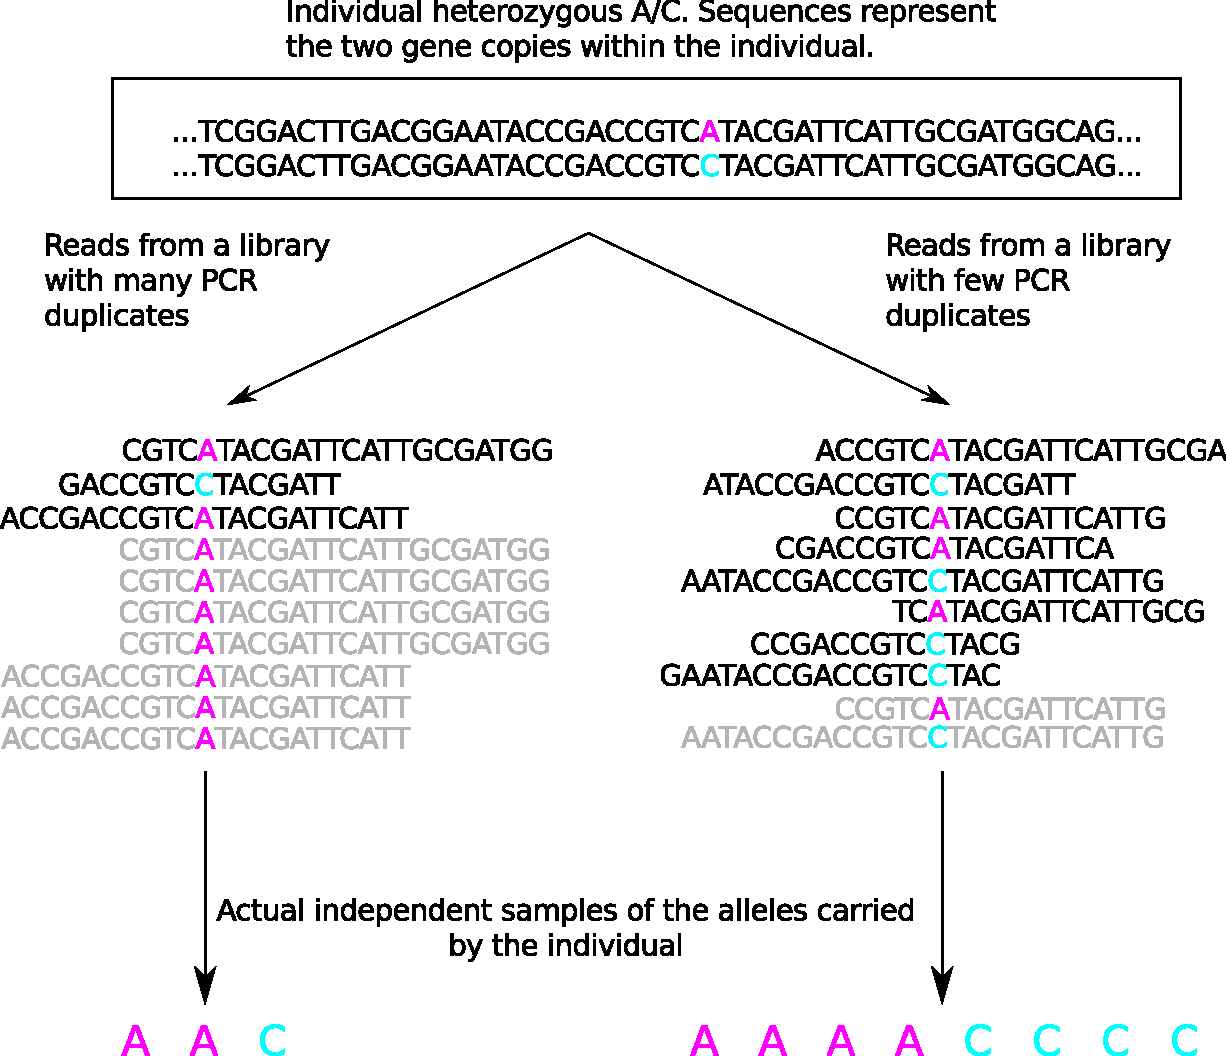
\includegraphics{figs/pcr-duplicates} 

}

\caption{An example of PCR duplicates.  Note that in paired end data, duplicates are identified by the lengths of both reads as well as the insert length.  This figure represents a simplified, "toy" situation, showing just single-end data.}\label{fig:pcr-duplicates}
\end{figure}

PCR duplicates occur during the library prep stage, and also are only possible for
fragments originating from the same individual sample. In other words, if you found
two different paired-end reads that mapped to the same location in the genome, but they
were from different individuals (i.e.~had different sample-specific DNA barcodes),
you would not suspect that they were PCR duplicates.
Likewise, DNA fragments from two different library preps, even if they came from the
same individuals (in the case that DNA from that individual had been prepared
in two separate libraries) would not be considered to be PCR duplicates.
(We should pause here to note what is considered a ``library prep.'' Basically,
if a batch of samples were all processed together in the same day with reagents
from the same kit, that is considered a single ``library prep.'')
Accordingly, when keeping track of read groups \emph{for the purposes of identifying PCR duplicates},
the most important information is which individuals the DNA came from
and which library preparation it was prepared in.

What we can conclude from this section is that, for downstream analyses,
we need a way to quickly (and efficiently, in terms of data storage space)
identify, for each read the:

\begin{itemize}
\tightlist
\item
  Sample it originated from
\item
  The library in which it was prepared for sequencing.
\item
  The flowcell that it was sequenced on.
\item
  The lane on that flowcell that it was sequenced on
\end{itemize}

This information can be strored in the alignment file using
read group information as described below.

\hypertarget{read-groups}{%
\section{Read Groups}\label{read-groups}}

We touched briefly on read groups in Section \ref{sam-headers}, where we
noted that the SAM file header can contain lines like this one:

\begin{verbatim}
@RG ID:HTYYCBBXX.1.CH_plate1_A01    SM:CH_plate1_A01    LB:Lib-1    PU:HTYYCBBXX.1.TCAATCCG+TTCGCAGT    PL:ILLUMINA
\end{verbatim}

The purpose of this line is to identify a read group that is named via the \texttt{ID} tag. In the above
case the read group is named \texttt{HTYYCBBXX.1.CH\_plate1\_A01}. The attributes of this read group are stored
using the remaining tags. Happily, those attributes mirror exactly what we might need to know to
identify PCR duplicates and to perform base quality score recalibration; namely:

\begin{itemize}
\tightlist
\item
  \texttt{SM} : give the name of the sample, \texttt{CH\_plate1\_A01}, the read is from,
\item
  \texttt{LB} : gives the name of the library prep, \texttt{Lib-1}, the read is from,
\item
  \texttt{PU} : gives the name of the flowcell, \texttt{HTYYCBBXX}, and the lane, \texttt{1}, the read is from.
\end{itemize}

It is important to note that this line in the SAM header is just a header line that gives
information about a particular read group that is found in the file. It is not, \emph{by itself}
giving you information about any particular read found in the alignment file. Read group information
about a particular read in the alignment file is given on the alignment line in a column (way off near the
end of the line typically) tagged with \texttt{RG:Z}. That column simply holds the \texttt{ID} of the read group
that the read belongs to. In this way, all the information that applies to the read--0i.e., the sample it
came from, (\texttt{SM}), the library prep it was in (\texttt{LB}), and information about the flowcell and lane (\texttt{PU})---can
be assigned to the read, \emph{without writing all of that information on every line in the alignment file}.
Accordingly, it should be obvious why the read group IDs must be unique across all the different
read groups (\texttt{@RG} tags) in a SAM/BAM file: the ID is used to identify all the other information
that goes along with that read, and is used to differentiate those different read groups!

You can download the first 100 lines (without the \texttt{@SQ} lines) of a SAM file that has 8 different
read groups in it \href{https://eriqande.github.io/eca-bioinf-handbook/downloads/CH_plate1_A01_mkdup-100-lines.sam}{here}.
Let's do that and have a look at it.

The way that read group information---particularly the platform unit, or \texttt{PU} information---is recorded
is dicated by which software will be used for downstream processing.
We describe the
conventions that are useful for
passing the aligned data to the Genome Analysis Toolkit (GATK), an extensive
and well-supported piece
of software developed by the Broad Institute. Currently, the convention for the
read group tags are these:

\begin{itemize}
\tightlist
\item
  \texttt{ID} : any string that uniquely identifies a read group. The user must make sure that
  these uniquely identify the read groups. If you have multiple samples, libraries, flowcells, and
  lanes, and easy way to ensure this is to just bung those all together in a format like
  \texttt{\{Sample\}.\{Library\}.\{Flowcell\}.\{Lane\}}, where the parts in curly braces should be replaced by the
  actual names of those items. As long as there is a \texttt{PU} field, however, you can make the ID
  anything you want, as long as it is unique for each read group.
\item
  \texttt{SM} : any string (no spaces please!) that serves as an identifier for the individual the sample
  was taken from. This is used to assign genotypes to indvididuals, so even if you have different
  ``samples'' from the same individual (i.e.~some blood and some tissue, prepped in different libraries;
  or an original extraction prepared in an earlier library and a later extraction prepared in a library
  for individuals that needed more sequening coverage after an initial sequencing run)
  you should still assign them \emph{all} the same \texttt{SM} tag because they are the same individual, and you will'
  want all of the DNA sequences from them to apply to calling genotypes for them.
\item
  \texttt{LB} : any string which gives the name of the library prep these reads were prepared in. If you prepped
  192 individuals in one day, they are all part of the same library.
\item
  \texttt{PU} : GATK expects this information to be given in a specific format. You can provide it as
  \texttt{\{Flowcell\}.\{Lane\}} (for example, \texttt{HTYYCBBXX.1}), but with later versions of the base quality score
  recalibration methods in GATK, it appears that it might be useful to also add information about
  the particular individual/library the read came from. It is suggested that this be done by
  including the barcode of reads, as \texttt{\{Flowcell\}.\{Lane\}.\{Barcode\}}, like
  \texttt{HTYYCBBXX.1.TCAATCCG+TTCGCAGT}.
\item
  \texttt{PL} : It is also important for base calibration to indicate what type of sequencer was used.
  Most of the time, currently, that will be \texttt{ILLUMINA}.
\end{itemize}

Usually, when you get data back from the sequencing center, it will be in a series
of different FASTQ files, each one containing reads from a single DNA sample well (on a plate
that you sent to them), that was sequenced on a certain lane on a given flow cell. The files
will often be named something like: \texttt{DPCh\_plate1\_C07\_S31\_L7\_R2.fq.gz} where the first part
gives a sample identifier, the part after the \texttt{L} gives the lane, and the part after the
\texttt{R} tells whether the file holds read 1 or read 2 of paired end reads. You can get the flowcell
name by looking at the sequence names inside the file (See Section \ref{illumina-ids}). You
will map the reads in each file separately, and when you do so, you will attach the read group
information to them (see below). Accordingly, it is a great idea to maintain a spreadsheet
that links the different files to the attributes and the read group information of the reads inside
them, like this:

\begin{verbatim}
index   file_prefix ID  PU  SM  PL  LB  Flowcell    Lane
1   DPCh_plate1_A01_S1_L1_R HTYYCBBXX.1.CH_plate1_A01   HTYYCBBXX.1.TCAATCCG+TTCGCAGT   CH_plate1_A01   ILLUMINA    Lib-1   HTYYCBBXX   1
2   DPCh_plate1_A01_S1_L2_R HTYYCBBXX.2.CH_plate1_A01   HTYYCBBXX.2.TCAATCCG+TTCGCAGT   CH_plate1_A01   ILLUMINA    Lib-1   HTYYCBBXX   2
3   DPCh_plate1_A01_S1_L3_R HTYYCBBXX.3.CH_plate1_A01   HTYYCBBXX.3.TCAATCCG+TTCGCAGT   CH_plate1_A01   ILLUMINA    Lib-1   HTYYCBBXX   3
4   DPCh_plate1_A01_S1_L4_R HTYYCBBXX.4.CH_plate1_A01   HTYYCBBXX.4.TCAATCCG+TTCGCAGT   CH_plate1_A01   ILLUMINA    Lib-1   HTYYCBBXX   4
5   DPCh_plate1_A01_S1_L5_R HTYYCBBXX.5.CH_plate1_A01   HTYYCBBXX.5.TCAATCCG+TTCGCAGT   CH_plate1_A01   ILLUMINA    Lib-1   HTYYCBBXX   5
6   DPCh_plate1_A01_S1_L6_R HTYYCBBXX.6.CH_plate1_A01   HTYYCBBXX.6.TCAATCCG+TTCGCAGT   CH_plate1_A01   ILLUMINA    Lib-1   HTYYCBBXX   6
7   DPCh_plate1_A01_S1_L7_R HTYYCBBXX.7.CH_plate1_A01   HTYYCBBXX.7.TCAATCCG+TTCGCAGT   CH_plate1_A01   ILLUMINA    Lib-1   HTYYCBBXX   7
8   DPCh_plate1_A01_S1_L8_R HTYYCBBXX.8.CH_plate1_A01   HTYYCBBXX.8.TCAATCCG+TTCGCAGT   CH_plate1_A01   ILLUMINA    Lib-1   HTYYCBBXX   8
9   DPCh_plate1_A02_S2_L1_R HTYYCBBXX.1.CH_plate1_A02   HTYYCBBXX.1.CGCTACAT+CGAGACTA   CH_plate1_A02   ILLUMINA    Lib-1   HTYYCBBXX   1
\end{verbatim}

In the exercise we will see how to use such a file to assign read groups when mapping.

\hypertarget{aligning-reads-with-bwa}{%
\section{\texorpdfstring{Aligning reads with \texttt{bwa}}{Aligning reads with bwa}}\label{aligning-reads-with-bwa}}

There are several programs for aligning reads to a reference genome. We focus on \texttt{bwa} which is
an industry standard aligner written by Heng Li and Richard Durbin \citep{liFastAccurateShort2009}. The name
stands for ``Burrows-Wheeler Aligner.'' We won't go deeply into the guts of this alignment algorithm, but we
will briefly state that nearly all alignment methods rely on pre-processing the reference genome into a
data-structure (like a suffix tree) that provides an \emph{index} which makes it fast to find the place in
a genome where a query sequence matches. Such indexes can take up a large amount of computer memory.
The Burrows-Wheeler Transform (BWT) provides a way of decreasing the size of such indexes. The BWT is an
operation that takes a sequence of characters (in this case DNA bases) and re-orders them so that similar
characters tend to appear together in long runs of the same character. Sequences with long runs of
the same character can be easily compressed to take up less space using \emph{run length encoding}, for example.
(We have already seen an example of run length encoding in the CIGAR string (Section \ref{cigar}), in which
runs of the same kind of alignment characteristic (Matches, Deletions, etc) where encoded by their type
and the length of the run.) The remarkable thing about the BWT is that it is \emph{invertible}: if someone gives
you a sequence and says that it is the result of applying the BWT to an original sequence, you can
actually recover the original sequence without any other information! The program \texttt{bwa} uses the BWT to
compress the index used for alignment so that it can easily fit into memory---even for very large genomes---on most any computer system, even a low-powered laptop produced in the last half decade.

\hypertarget{indexing-the-genome-for-alignment}{%
\subsection{Indexing the genome for alignment}\label{indexing-the-genome-for-alignment}}

As the foregoing discussion suggests, it is necessary to index a genome before aligning to it
with \texttt{bwa}. This is a step that only needs to be done once, since the process creates an index
that is stored on the hard drive alongside the genome. So, after you download a reference genome,
before you can start aligning sequences to it, you must index it using \texttt{bwa}. The syntax for this
is very straightforward:

\begin{Shaded}
\begin{Highlighting}[]
\ExtensionTok{bwa}\NormalTok{ index path-to-genome}
\end{Highlighting}
\end{Shaded}

For example:

\begin{Shaded}
\begin{Highlighting}[]
\ExtensionTok{bwa}\NormalTok{ index genome/GCA_002872995.1_Otsh_v1.0_genomic.fna.gz}
\end{Highlighting}
\end{Shaded}

The reference genome must be stored as a FASTA file (Section \ref{fasta}), which can
be compressed using \texttt{gzip}. (In the above example, the \texttt{.fna.gz} prefix means that the
file is a FASTA file of nucleotides (\texttt{.fna}) and has been gzipped (\texttt{.gz})).

This process may take several hours, depending upon the size of the reference
genome. When it is complete, several new files with names that are the
orginal reference genome file plus several extensions will have been produced
and saved in the same directory as the reference genome. In the above example,
after indexing, a long listing of the directory with the genome file in it
shows these files:

\begin{verbatim}
% ls -hl
total 3.8G
-rw-rw-r-- 1 eanderson eanderson 704M Mar  5 00:08 GCA_002872995.1_Otsh_v1.0_genomic.fna.gz
-rw-rw-r-- 1 eanderson eanderson 4.4M Mar  5 00:47 GCA_002872995.1_Otsh_v1.0_genomic.fna.gz.amb
-rw-rw-r-- 1 eanderson eanderson 2.1M Mar  5 00:47 GCA_002872995.1_Otsh_v1.0_genomic.fna.gz.ann
-rw-rw-r-- 1 eanderson eanderson 2.3G Mar  5 00:47 GCA_002872995.1_Otsh_v1.0_genomic.fna.gz.bwt
-rw-rw-r-- 1 eanderson eanderson 579M Mar  5 00:47 GCA_002872995.1_Otsh_v1.0_genomic.fna.gz.pac
-rw-rw-r-- 1 eanderson eanderson 1.2G Mar  5 00:58 GCA_002872995.1_Otsh_v1.0_genomic.fna.gz.sa
\end{verbatim}

The first file is the original gzipped compressed reference genome, and the remaining files
are all part of the index. Note that the index files occupy considerably more space than
the original reference file (but not so much as they would if the BWT were not used to
reduce the size of the index).

If you ever wonder whether you have indexed a certain reference genome with \texttt{bwa}, it is
a simple matter to go to the directory holding the reference genome and see what other files
are there. If you find files with the same name, but having the suffixes, \texttt{.amb}, \texttt{.ann}, \texttt{.bwt}, \texttt{.pac}
and \texttt{.sa}, that means that the reference genome \emph{has} already been indexed.

\hypertarget{mapping-reads-with-bwa-mem}{%
\subsection{\texorpdfstring{Mapping reads with \texttt{bwa\ mem}}{Mapping reads with bwa mem}}\label{mapping-reads-with-bwa-mem}}

Once the reference genome has been indexed, you are ready to align reads to
it. The program \texttt{bwa} includes several different alignment algorithms. For paired-end Illumina data,
the best available \texttt{bwa} algorithm, today, is the \texttt{mem} algorithm. The syntax is very simple. While there
are many options available to tune the parameters used for alignment, the default values
usually give good performance. Thus, at its
simplest, \texttt{bwa\ mem} simply takes three file arguments:

\begin{Shaded}
\begin{Highlighting}[]
\ExtensionTok{bwa}\NormalTok{ mem   path-to-reference-genome   path-to-read1-fastq-file   path-to-read2-fastq-file}
\end{Highlighting}
\end{Shaded}

An example might look like:

\begin{Shaded}
\begin{Highlighting}[]
\ExtensionTok{bwa}\NormalTok{ mem genome/GCA_002872995.1_Otsh_v1.0_genomic.fna.gz fastqs/DPCh_plate1_A01_S1_L1_R1.fq.gz fastqs/DPCh_plate1_A01_S1_L1_R2.fq.gz}
\end{Highlighting}
\end{Shaded}

\texttt{bwa\ mem} prints progress messages to \emph{stderr} and prints its output in SAM format to \emph{stdout}. The read alignments
come spewing out in the order they are listed in the FASTQ files, such that each read and its
paired-end mate appear in adjacent rows in the output. It's all super simple!

\hypertarget{hold-it-right-there-buddy-what-about-the-read-groups}{%
\subsection{Hold it Right There, Buddy! What about the Read Groups?}\label{hold-it-right-there-buddy-what-about-the-read-groups}}

Indeed! It is during the mapping with \texttt{bwa\ mem} that we must include
read group tags for our reads. This is straightforward if the pair of
FASTQ files contains reads that are all from a single read group, we
merely have to give the read group information that we want to see as the
argument to the \texttt{-R} option of \texttt{bwa\ mem}. This argument must be a single
token on the command line, so, if it does not include spaces or other whitespace
it can be supplied unquoted; however, it is usually safer to quote the argument on
the command line. The tabs that occur between read group tags are given as \texttt{\textbackslash{}t}
in the argument to the \texttt{-R} option.

Thus, in the \texttt{bwa\ mem} documentation, the example invocation of the \texttt{-R} option
shows it single quoted as \texttt{\textquotesingle{}@RG\textbackslash{}tID:foo\textbackslash{}tSM:bar\textquotesingle{}}. In other words, you pass it
the read group header line, complete with the \texttt{@RG} header tag, encoding the tabs
between identifiers with \texttt{\textbackslash{}t}. What this example does not make clear is that
you can also use \emph{double quotes} around that argument. Double quotes, you will recall,
allow variable substitution (Section \ref{quotes-and-var-subs}) to occur inside them.
So, in your own scripts, especially when cycling over very many different pairs of
FASTQ files, it is extremely useful to be able to define the values of the read group
tags, and then supply them on the command line. Coarsely this would look like:

\begin{Shaded}
\begin{Highlighting}[]
\VariableTok{ID=}\NormalTok{HTYYCBBXX.1.CH_plate1_A01}
\VariableTok{SM=}\NormalTok{CH_plate1_A01}
\VariableTok{LB=}\NormalTok{Lib-1}
\VariableTok{PU=}\NormalTok{HTYYCBBXX.1.TCAATCCG+TTCGCAGT}
\VariableTok{PL=}\NormalTok{ILLUMINA}

\ExtensionTok{bwa}\NormalTok{ mem -R }\StringTok{"@RG\textbackslash{}tID:}\VariableTok{$ID}\StringTok{\textbackslash{}tSM:}\VariableTok{$SM}\StringTok{\textbackslash{}tLB:}\VariableTok{$LB}\StringTok{\textbackslash{}tPU:}\VariableTok{$PU}\StringTok{\textbackslash{}tPL:}\VariableTok{$PL}\StringTok{"}\NormalTok{  genome.fasta  file_R1.fq file_R2.fq}
\end{Highlighting}
\end{Shaded}

However, you would probably want some way of assigning the values of the
shell variables \texttt{ID}, \texttt{SM}, etc., programmatically, perhaps from the spreadsheet
that holds all that information. The exercise this week shows one example of that
using \texttt{awk} and a TAB-delimited spreadsheet.

\hypertarget{processing-alignment-output-with-samtools}{%
\section{\texorpdfstring{Processing alignment output with \texttt{samtools}}{Processing alignment output with samtools}}\label{processing-alignment-output-with-samtools}}

Doing the alignment with \texttt{bwa\ mem} is only the first step of getting data ready to do
variant calling. Once the SAM format data comes out of \texttt{bwa\ mem}, a number of things
must happen to it before it can be used for variant calling:

\begin{enumerate}
\def\labelenumi{\arabic{enumi}.}
\tightlist
\item
  It must be converted to BAM format (the compressed binary companion format to SAM)
\item
  Additional information about mate pairs might need to be attached to sequences
\item
  You must sort the BAM files from the original ordering produced by \texttt{bwa\ mem} into a
  \emph{coordinate-ordered} format, in which the reads are sorted by where they appear within the
  reference genome.
\item
  If you started with multiple pairs of FASTQ files for a single individual (i.e.~from different lanes
  or from different sequencing runs or libraries) you might want to merge those all into a single BAM
  file.
\item
  You might want to mark PCR duplicates as such in the BAM file.
\item
  Finally when you have your BAM file all ready for variant calling, you typically
  will need to index it for rapid access by the variant caller program.
\end{enumerate}

Phew! That is a lot of steps! Fortunately, there is a single ``go-to'' program (one-stop shopping!)
that can manage all of that for you. It is the program \texttt{samtools}, brought to you by the
same people who developed the SAM/BAM formats \citep{liSequenceAlignmentMap2009} and the \texttt{bwa} aligner
(and \texttt{bcftools} for that matter). If you want to get anywhere in bioinformatics, it is
important to become good friends with \texttt{samtools}.

The program \texttt{samtools} includes a large number of different subcommands.
We will cover just a few of them, here, that are used in our typical paired-end workflow,
and in a somewhat cursory fashion, including only the most commonly used options.
All readers are encouraged to completely read the online \href{http://www.htslib.org/doc/samtools.html}{manual page}
for samtools for a complete account of its uses.

In the samtools manual. The usage patterns of the subcommands can broadly be categorized into
two groups:

\begin{enumerate}
\def\labelenumi{\arabic{enumi}.}
\item
  Subcommands that explicitly require an argument that gives the name of an output file.
  These subcommands are usually described like this:

\begin{Shaded}
\begin{Highlighting}[]
\ExtensionTok{samtools}\NormalTok{ subcommand [options] out.bam in.bam}
\end{Highlighting}
\end{Shaded}

  where an output file is explicitly called for. These commands
  \emph{do not write output to stdout}! They must be given an output file name. It is
  \emph{not possible} to pipe output from one of these subcommands to another program or utility.
\item
  Subcommands that don't explicitly require an argument giving an output file:

\begin{Shaded}
\begin{Highlighting}[]
\ExtensionTok{samtools}\NormalTok{ subcommand [options] in.bam}
\end{Highlighting}
\end{Shaded}

  These subcommands write their output to stdout, and that output can be piped into other programs or can
  be redirected into a file (some also provide a \texttt{-o\ file} option to write output to \texttt{file} rather than
  to stdout.)
\end{enumerate}

In short, if the syntax of the subcommand explicitly calls for an output file on the command line (not as part
of a \texttt{-o\ file} option), then that subcommand does not write its output to \emph{stdout} and you can't pipe it into
the next part of your pipeline.

On the other hand, if you can write output from samtools to \emph{stdout}, you might be interested in knowing
how you can pipe that into the input for another \texttt{samtools} subcommand. Rejoice! There is a syntactically
economical and lovely way to do that. Any subcommand which expects a single input file will be described
like:

\begin{Shaded}
\begin{Highlighting}[]
\ExtensionTok{samtools}\NormalTok{ subcommand [options]  in.bam}
\end{Highlighting}
\end{Shaded}

You would typically put the path to the input file in the place of \texttt{in.bam} there.
However, if you put \texttt{-} in place of \texttt{in.bam} then samtools will take input for
\texttt{in.bam} from \emph{stdin}.

So, for example, you can do something like this:

\begin{Shaded}
\begin{Highlighting}[]
\ExtensionTok{bwa}\NormalTok{ mem genome.fna R1.fq R2.fq }\KeywordTok{|}
  \ExtensionTok{samtools}\NormalTok{ view -b -  }\KeywordTok{|}\NormalTok{   # }\ExtensionTok{convert}\NormalTok{ the SAM output from bwa mem into BAM format}
  \ExtensionTok{samtools}\NormalTok{ fixmate -m - output_file  # take stdin as the input and write output to output_file}
\end{Highlighting}
\end{Shaded}

You can download an 11 Mb BAM file to play around with \href{https://eriqande.github.io/eca-bioinf-handbook/downloads/CH_plate1_A01_mkdup.bam}{here}.
If you are on your HPCC and want to download it, you can use:

\begin{Shaded}
\begin{Highlighting}[]
\FunctionTok{wget}\NormalTok{ https://eriqande.github.io/eca-bioinf-handbook/downloads/CH_plate1_A01_mkdup.bam}
\end{Highlighting}
\end{Shaded}

\hypertarget{samtools-subcommands}{%
\subsection{\texorpdfstring{\texttt{samtools} subcommands}{samtools subcommands}}\label{samtools-subcommands}}

\hypertarget{samtools-view}{%
\subsubsection{\texorpdfstring{\texttt{samtools\ view}}{samtools view}}\label{samtools-view}}

The major workhorse. Used for viewing BAM files (-h/-H) and also for converting
SAM files to BAM files (the latter being necessary, or, at least prudent, for all
downstream processing).

\hypertarget{samtools-fixmate}{%
\subsubsection{\texorpdfstring{\texttt{samtools\ fixmate}}{samtools fixmate}}\label{samtools-fixmate}}

Add information about mates needed to identify PCR duplicates. Mates must be adjacent to
one another in the output. Best to run this right after alignment.

\hypertarget{samtools-sort}{%
\subsubsection{\texorpdfstring{\texttt{samtools\ sort}}{samtools sort}}\label{samtools-sort}}

Put things in a BAM file in order of placement in the reference genome. This must be done for
most downstream operations. Especially for merging and for marking duplicates.

\hypertarget{samtools-merge}{%
\subsubsection{\texorpdfstring{\texttt{samtools\ merge}}{samtools merge}}\label{samtools-merge}}

Combine the contents of sorted BAM files.

\hypertarget{samtools-markdup}{%
\subsubsection{\texorpdfstring{\texttt{samtools\ markdup}}{samtools markdup}}\label{samtools-markdup}}

Mark PCR (or optical) duplicates.

\hypertarget{samtools-stats}{%
\subsubsection{\texorpdfstring{\texttt{samtools\ stats}}{samtools stats}}\label{samtools-stats}}

Summary information about the alignments.

\hypertarget{samtools-idxstats}{%
\subsubsection{\texorpdfstring{\texttt{samtools\ idxstats}}{samtools idxstats}}\label{samtools-idxstats}}

Summary information about the SAM flags of the alignments.

\hypertarget{samtools-bedcov}{%
\subsubsection{\texorpdfstring{\texttt{samtools\ bedcov}}{samtools bedcov}}\label{samtools-bedcov}}

Calculate coverage of different regions in the reference genome.

\hypertarget{boneyard-below-here}{%
\section{BONEYARD BELOW HERE}\label{boneyard-below-here}}

\hypertarget{preprocess}{%
\section{Preprocess ?}\label{preprocess}}

Will have a bit about sequence pre-processing (with WGS data it already
comes demultiplexed, so maybe we can hold off on this until we get to
RAD data). No, we need to talk about trimming and maybe slicing. Perhaps
put that in a separate chapter of ``preliminaries''

\hypertarget{quick-notes-to-self-on-chaining-things}{%
\section{Quick notes to self on chaining things:}\label{quick-notes-to-self-on-chaining-things}}

When using samtools markdup you can do like this:

\begin{Shaded}
\begin{Highlighting}[]
\CommentTok{# first step}
\ExtensionTok{bwa}\NormalTok{ mem chinook-play/chinook-genome-idx/GCA_002872995.1_Otsh_v1.0_genomic.fna.gz chr32-160-chinook/laned/DPCh_plate1_A01_S1_L1_R1.fq chr32-160-chinook/laned/DPCh_plate1_A01_S1_L1_R2.fq }\KeywordTok{|} \KeywordTok{\textbackslash{}}
    \ExtensionTok{samtools}\NormalTok{ view -b -1 - }\KeywordTok{|} \KeywordTok{\textbackslash{}}
    \ExtensionTok{samtools}\NormalTok{ fixmate -m -O BAM - fixed.bam}
    
\CommentTok{# unfortunately, fixmate can't write to stdout.}
\CommentTok{# then, after this, we have to sort it into coordinate order and}
\CommentTok{# markdup them.}
\ExtensionTok{samtools}\NormalTok{ sort fixed.bam }\KeywordTok{|} \ExtensionTok{samtools}\NormalTok{ markdup - marked.bam}

\CommentTok{# after that, fixed.bam could get tossed.}
\end{Highlighting}
\end{Shaded}

\hypertarget{merging-bam-files}{%
\section{Merging BAM files}\label{merging-bam-files}}

There is a lot of discussion on biostars about how samtools does not reconstruct the
\texttt{@RG} dictionary. But I think that this must be a problem with an older version. The
newer version works just fine. That said, Picard's MergeSamFiles seems to be just about
as fast (in fact, faster. For a comparably sized file it took 25 minutes, and gives informative
output telling you where it is at). And samtools merge is at well over 30 and only about
3/4 of the way through. Ultimately it took 37 minutes. Might have been on a slower machine\ldots{}

However, if you have sliced your fastqs and mapped each separately, then
samtools let's you not alter duplicate read group IDs, and so you can merge
those all together faithfully, as I did in the impute project. Cool.

\hypertarget{divide-and-conquer-strategies}{%
\section{Divide and Conquer Strategies}\label{divide-and-conquer-strategies}}

At the end of each of these chapters, I think I will
have a special section talking about ways that things can be divided
up so that you can do it quickly, or at least, within time limits
on your cluster.

\hypertarget{variant-calling-with-gatk}{%
\chapter{Variant calling with GATK}\label{variant-calling-with-gatk}}

Standard stuff here.

Big focus on parallelizing.

\hypertarget{bioinformatics-for-rad-seq-data-with-and-without-a-reference-genome}{%
\chapter{Bioinformatics for RAD seq data with and without a reference genome}\label{bioinformatics-for-rad-seq-data-with-and-without-a-reference-genome}}

We've gotta get our hands dirty with RAD and STACKS.

For some applications (like massive salamander genomes) this is the only
way forward, at the moment. Can be useful, but is also
fraught with peril.

Discuss all the problems, and strategies for dealing with them.

Note that stacks2 is a lot better than things were before. And, you can use
a reference genome with them.

Amanda Stahlke gave a nice practical example at ConGen. Found all the materials
on box through the link that Brian Hand gave me (in my email.)

That will be worth running through closely and carefully. Note that stacks2's denovo\_map.pl script
now takes all the tsv output and puts it into a series of bams.

\hypertarget{processing-amplicon-sequencing-data}{%
\chapter{Processing amplicon sequencing data}\label{processing-amplicon-sequencing-data}}

Super high read depths can cause problems for some pipelines.

I am going to mostly focus on short amplicons that are less than the
number of sequencing cycles, and how we create microhaps out of those, and
the great methods we have for visualizing and curating those.

\hypertarget{genome-annotation}{%
\chapter{Genome Annotation}\label{genome-annotation}}

I don't intend this to be a treatise on how to actually annotate a genome.
Presumably, that is a task that involves feeding a genome and a lot of mRNA
transcripts into a pipeline that then makes gene models, etc. I guess I could
talk a little about that process, 'cuz it would be fun to learn more about it.

However, I will be more interested in understanding what annotation data look like
(i.e.~in a GFF file) and how to associate it with SNP data (i.e.~using snpEff).

The GFF format is a distinctly hierarchical format, but it is still tabular,
it is not in XML, thank god! 'cuz it is much easier to parse in tabular format.

You can fiddle it with bedtools.

Here is an idea for a fun thing for me to do: Take a big chunk of chinook GFF
(and maybe a few other species), and then figure out who the parents are of each of the
rows, and then make a graph (with dot) showing all the different links (i.e.~gene -\textgreater{} mRNA -\textgreater{} exon -\textgreater{} CDS)
etc, and count up the number of occurrences of each, in order to get a sense of what
sorts of hierarchies a typical GFF file contains.

\hypertarget{whole-genome-alignment-strategies}{%
\chapter{Whole genome alignment strategies}\label{whole-genome-alignment-strategies}}

Basically want to talk about situations

\hypertarget{mapping-of-scaffolds-to-a-closely-related-genome}{%
\section{Mapping of scaffolds to a closely related genome}\label{mapping-of-scaffolds-to-a-closely-related-genome}}

I basically want to get my head fully around how SatsumaSynteny works.

After that, we might as well talk about how to get in and modify a VCF file to reflect the new positions and such. (It seems we could even add something to the INFO field that listed its position in the old scaffold system. awk + vcftools sort seems like it might be the hot ticket.)

\hypertarget{obtaining-ancestral-states-from-an-outgroup-genome}{%
\section{Obtaining Ancestral States from an Outgroup Genome}\label{obtaining-ancestral-states-from-an-outgroup-genome}}

For many analyses it is helpful (or even necessary) to have a guess at the ancestral
state of each DNA base in a sequence. These ancestral states are often guessed to be the
state of a closely related (but outgroup) species. The idea there is that it is rare for
the same nucleotide to experience a substitution (or mutation) in each species, so the
base carried by the outgroup is assumed to be the ancestral sequence.

So, that is pretty straightforward conceptually, but there is plenty of hardship
along the way to do this. There are two main problems:

\begin{enumerate}
\def\labelenumi{\arabic{enumi}.}
\item
  Aligning the outgroup genome (as a query) to the target genome. This typically
  produces a multiple alignment format (MAF) file. So, we have to understand that
  file format. (read about it \href{http://genome.ucsc.edu/FAQ/FAQformat\#format5}{here}, on the
  UCSC genome browser site.) A decent program to do this alignment exercise appears to
  be \href{http://www.bx.psu.edu/miller_lab/dist/README.lastz-1.02.00/README.lastz-1.02.00a.html}{LASTZ}
\item
  Then, you might have to convert the MAF file to a fasta file to feed into something
  like ANGSD. It seems that Dent Earl has some tools that might to do this \href{https://github.com/dentearl/mafTools}{hhttps://github.com/dentearl/mafTools}. Also, the ANGSD github site has a \href{https://github.com/ANGSD/maf2fasta}{maf2fasta} program, though no
  documentation to speak of. Or you might just go ahead and write an awk script to do it.
  Galaxy has a website that will do it: \url{http://mendel.gene.cwru.edu:8080/tool_runner?tool_id=MAF_To_Fasta1}, and there is an alignment too called mugsy
  that has a perl script associated with it that will do it: \url{ftp://188.44.46.157/mugsy_x86-64-v1r2.3/maf2fasta.pl}
  Note that the fasta file for ancestral sequence used by ANGSD just seems to have Ns in the places that don't have alignments.
\end{enumerate}

It will be good to introduce people to those ``dotplots'' that show alignments.

Definitely some discussion of seeding and gap extensions, etc. The LASTZ web page has a
really nice explanation of these things.

The main take home from my explorations here is that there is no way to just toss two
genomes into the blender with default setting and expect that you are going to get
something reasonable out of that. There is a lot of experimentation, it seems to me, and
you really need to know what all the options are (this might be true of just about
everything in NGS analysis, but in many cases people just use the defaults\ldots{}.)

\hypertarget{using-lastz-to-align-coho-to-the-chinook-genome}{%
\subsection{Using LASTZ to align coho to the chinook genome}\label{using-lastz-to-align-coho-to-the-chinook-genome}}

First, compile it:

\begin{Shaded}
\begin{Highlighting}[]
\CommentTok{# in: /Users/eriq/Documents/others_code/lastz-1.04.00}
\FunctionTok{make}
\FunctionTok{make}\NormalTok{ install}

\CommentTok{# then I linked those (in bin) to myaliases}
\end{Highlighting}
\end{Shaded}

Refreshingly, this has almost no dependencies, and the compilation is super easy.

Now, let's find the coho chromomsome that corresponds to omy28 on NCBI. We can get this
with curl:

\begin{Shaded}
\begin{Highlighting}[]
\CommentTok{# in: /tmp}
\ExtensionTok{curl}\NormalTok{ ftp://ftp.ncbi.nlm.nih.gov/genomes/all/GCA/002/021/735/GCA_002021735.1_Okis_V1/GCA_002021735.1_Okis_V1_assembly_structure/Primary_Assembly/assembled_chromosomes/FASTA/chrLG28.fna.gz -o coho-28.fna.gz}
\FunctionTok{gunzip}\NormalTok{ coho-28.fna.gz}
\end{Highlighting}
\end{Shaded}

Then, let's also pull that chromosome out of the chinook genome we have:

\begin{Shaded}
\begin{Highlighting}[]
\CommentTok{# in /tmp}
\ExtensionTok{samtools}\NormalTok{ faidx  ~/Documents/UnsyncedData/Otsh_v1.0/Otsh_v1.0_genomic.fna NC_037124.1 }\OperatorTok{>}\NormalTok{ chinook-28.fna }
\end{Highlighting}
\end{Shaded}

Cool, now we should be able to run that:

\begin{Shaded}
\begin{Highlighting}[]
\BuiltInTok{time}\NormalTok{ lastz chinook-28.fna coho-28.fna --notransition --step=20 --nogapped --ambiguous=iupac --format=maf }\OperatorTok{>}\NormalTok{ chin28_vs_coho28.maf}

\ExtensionTok{real}\NormalTok{    0m14.449s}
\ExtensionTok{user}\NormalTok{    0m14.198s}
\ExtensionTok{sys}\NormalTok{ 0m0.193s}
\end{Highlighting}
\end{Shaded}

OK, that is ridiculously fast. How about we make a file that we can plot in R?

\begin{Shaded}
\begin{Highlighting}[]
\BuiltInTok{time}\NormalTok{ lastz chinook-28.fna coho-28.fna --notransition --step=20 --nogapped --ambiguous=iupac --format=rdotplot }\OperatorTok{>}\NormalTok{ chin28_vs_coho28.rdp}
\end{Highlighting}
\end{Shaded}

I copied that to \texttt{inputs} so we can plot it:

\begin{Shaded}
\begin{Highlighting}[]
\NormalTok{dots <-}\StringTok{ }\NormalTok{readr}\OperatorTok{::}\KeywordTok{read_tsv}\NormalTok{(}\StringTok{"inputs/chin28_vs_coho28.rdp.gz"}\NormalTok{)}
\end{Highlighting}
\end{Shaded}

\begin{verbatim}
## Parsed with column specification:
## cols(
##   NC_037124.1 = col_double(),
##   CM007745.1 = col_double()
## )
\end{verbatim}

\begin{Shaded}
\begin{Highlighting}[]
\KeywordTok{plot}\NormalTok{(dots,}\DataTypeTok{type=}\StringTok{"l"}\NormalTok{)}
\end{Highlighting}
\end{Shaded}

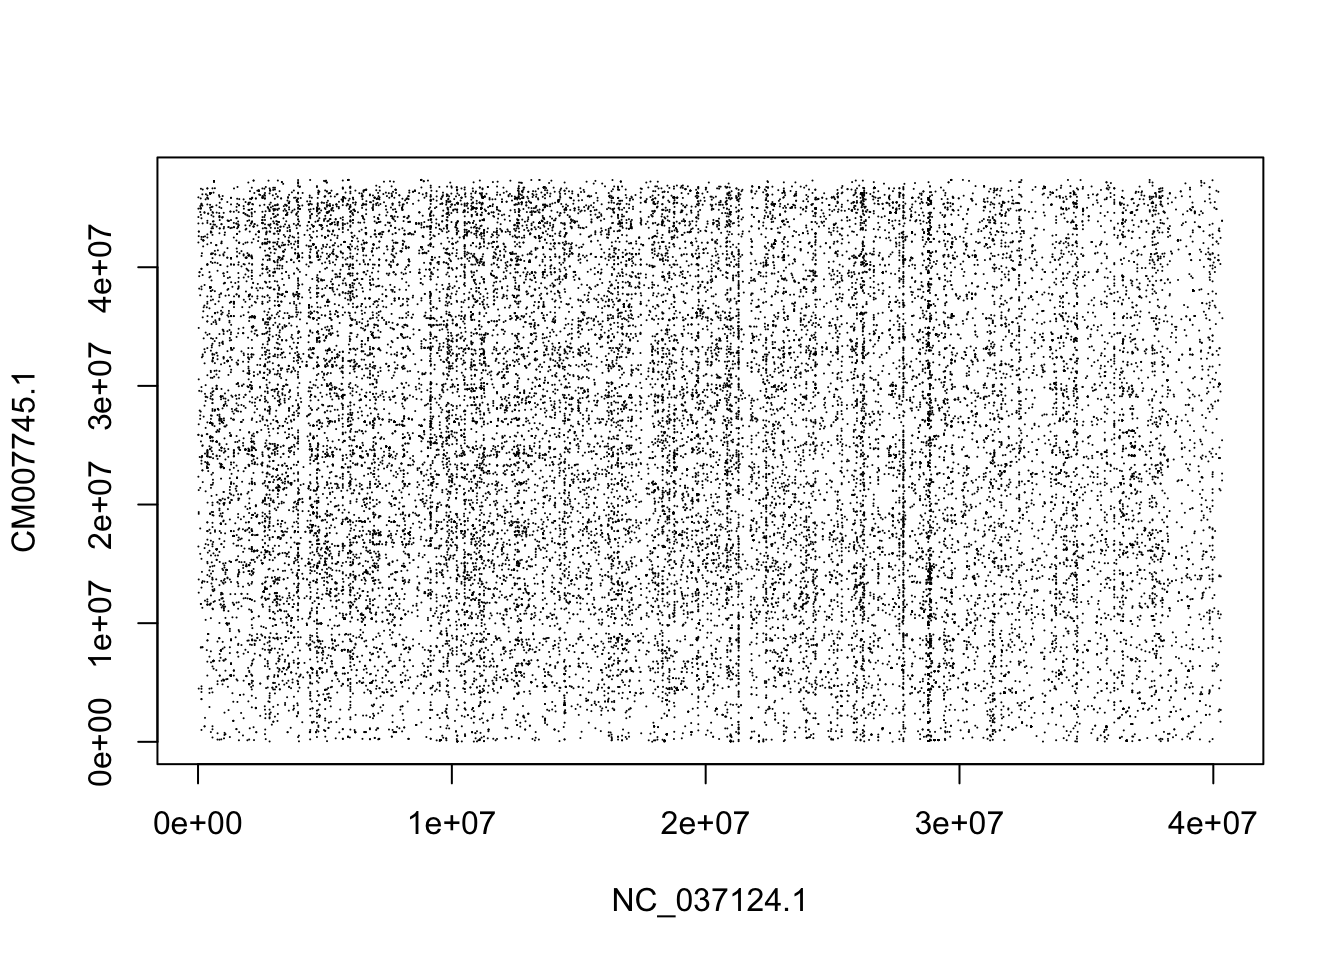
\includegraphics{eca-bioinf-handbook_files/figure-latex/unnamed-chunk-68-1.pdf}

OK, clearly what we have there is just a bunch of repetitive bits. I think we must not have the same chromosomes in the two species.

So, let's put LG28 in coho against the whole chinook genome. Note the use of the
bracketed ``multiple'' in there to let it know that there are multiple sequences in there
that should get catenated together.

\begin{Shaded}
\begin{Highlighting}[]
\BuiltInTok{time}\NormalTok{ lastz ~/Documents/UnsyncedData/Otsh_v1.0/Otsh_v1.0_genomic.fna[multiple]  coho-28.fna --notransition --step=20 --nogapped --ambiguous=iupac --format=maf }\OperatorTok{>}\NormalTok{ chin_vs_coho28.maf}

\ExtensionTok{FAILURE}\NormalTok{: in load_fasta_sequence for /Users/eriq/Documents/UnsyncedData/Otsh_v1.0/Otsh_v1.0_genomic.fna, sequence length 2,147,437,804+64,310 exceeds maximum (2,147,483,637)}
\end{Highlighting}
\end{Shaded}

No love there. But that chinook genome has a lot of short scaffolds in there too, I think.

Maybe we could just try LG1. Nope. How about we toss every coho LG against LG1 from chinook\ldots{}

\begin{Shaded}
\begin{Highlighting}[]
\CommentTok{# let's get the first 10 linkage groups from coho:}
\KeywordTok{for} \ExtensionTok{i}\NormalTok{ in }\DataTypeTok{\{1..10\}}\KeywordTok{;} \KeywordTok{do} \ExtensionTok{curl}\NormalTok{ ftp://ftp.ncbi.nlm.nih.gov/genomes/all/GCA/002/021/735/GCA_002021735.1_Okis_V1/GCA_002021735.1_Okis_V1_assembly_structure/Primary_Assembly/assembled_chromosomes/FASTA/chrLG}\VariableTok{$\{i\}}\NormalTok{.fna.gz -o coho-}\VariableTok{$\{i\}}\NormalTok{.fna.gz}\KeywordTok{;} \FunctionTok{gunzip}\NormalTok{ coho-}\VariableTok{$\{i\}}\NormalTok{.fna.gz}\KeywordTok{;} \BuiltInTok{echo} \VariableTok{$i}\KeywordTok{;} \KeywordTok{done} 

\CommentTok{# now lets try aligning those to the chinook}
\KeywordTok{for} \ExtensionTok{i}\NormalTok{ in }\DataTypeTok{\{1..10\}}\KeywordTok{;} \KeywordTok{do} \BuiltInTok{time}\NormalTok{ lastz chinook-1.fna coho-}\VariableTok{$\{i\}}\NormalTok{.fna --notransition --step=20 --nogapped --ambiguous=iupac --format=rdotplot }\OperatorTok{>}\NormalTok{ chinook1_vs_coho}\VariableTok{$\{i\}}\NormalTok{.rdp}\KeywordTok{;} \BuiltInTok{echo} \StringTok{"Done with }\VariableTok{$i}\StringTok{"}\KeywordTok{;} \KeywordTok{done}
\end{Highlighting}
\end{Shaded}

Nothing looked good until I got to coho LG10:

\begin{Shaded}
\begin{Highlighting}[]
\NormalTok{dots <-}\StringTok{ }\NormalTok{readr}\OperatorTok{::}\KeywordTok{read_tsv}\NormalTok{(}\StringTok{"inputs/chinook1_vs_coho10.rdp.gz"}\NormalTok{)}

\KeywordTok{plot}\NormalTok{(dots,}\DataTypeTok{type=}\StringTok{"l"}\NormalTok{)}
\end{Highlighting}
\end{Shaded}

There is clearly a big section that aligns there. But, we clearly are going to need to
clean up all the repetive crap, etc on these alignments.

\hypertarget{try-on-the-chinook-chromosomes}{%
\subsection{Try on the chinook chromosomes}\label{try-on-the-chinook-chromosomes}}

So, it crapped out on the full Chinook fasta. Note that I could modify the code (or compile it with a \texttt{-D}): check this out in sequences.h:

\begin{Shaded}
\begin{Highlighting}[]
\CommentTok{//  Sequence lengths are normally assumed to be small enough to fit into a}
\CommentTok{//  31-bit integer.  This gives a maximum length of about 2.1 billion bp, which}
\CommentTok{//  is half the length of a (hypothetical) monoploid human genome.  The}
\CommentTok{//  programmer can override this at compile time by defining max_sequence_index}
\CommentTok{//  as 32 or 63.}
\end{Highlighting}
\end{Shaded}

But, for now, I think I will just go for the assembled chromosomes only:

\begin{Shaded}
\begin{Highlighting}[]
\CommentTok{# just get the well assembled chromosomes (about 1.7 Gb)}
\CommentTok{# in /tmp}
\ExtensionTok{samtools}\NormalTok{ faidx ~/Documents/UnsyncedData/Otsh_v1.0/Otsh_v1.0_genomic.fna }\VariableTok{$(}\FunctionTok{awk} \StringTok{'/^NC/ \{printf("%s ", $1)\}'}\NormalTok{  ~/Documents/UnsyncedData/Otsh_v1.0/Otsh_v1.0_genomic.fna.fai}\VariableTok{)} \OperatorTok{>}\NormalTok{ chinook_nc_chroms.fna}

\CommentTok{# then try tossing coho 1 against that:}
\BuiltInTok{time}\NormalTok{ lastz chinook_nc_chroms.fna[multiple]  coho-1.fna --notransition --step=20 --nogapped --ambiguous=iupac --format=rdotplot }\OperatorTok{>}\NormalTok{ chin_nc_vs_coho1.rdp}

\CommentTok{# that took about 7 minutes}
\ExtensionTok{real}\NormalTok{    6m33.411s}
\ExtensionTok{user}\NormalTok{    6m28.391s}
\ExtensionTok{sys}\NormalTok{ 0m4.121s}
\end{Highlighting}
\end{Shaded}

Here is what the figure looks like. It is clear that the bulk of Chromosome 1
in coho aligns for long distances to two different chromosomes in Chinoook (likely
paralogs?). This is complex!

\begin{figure}
\centering
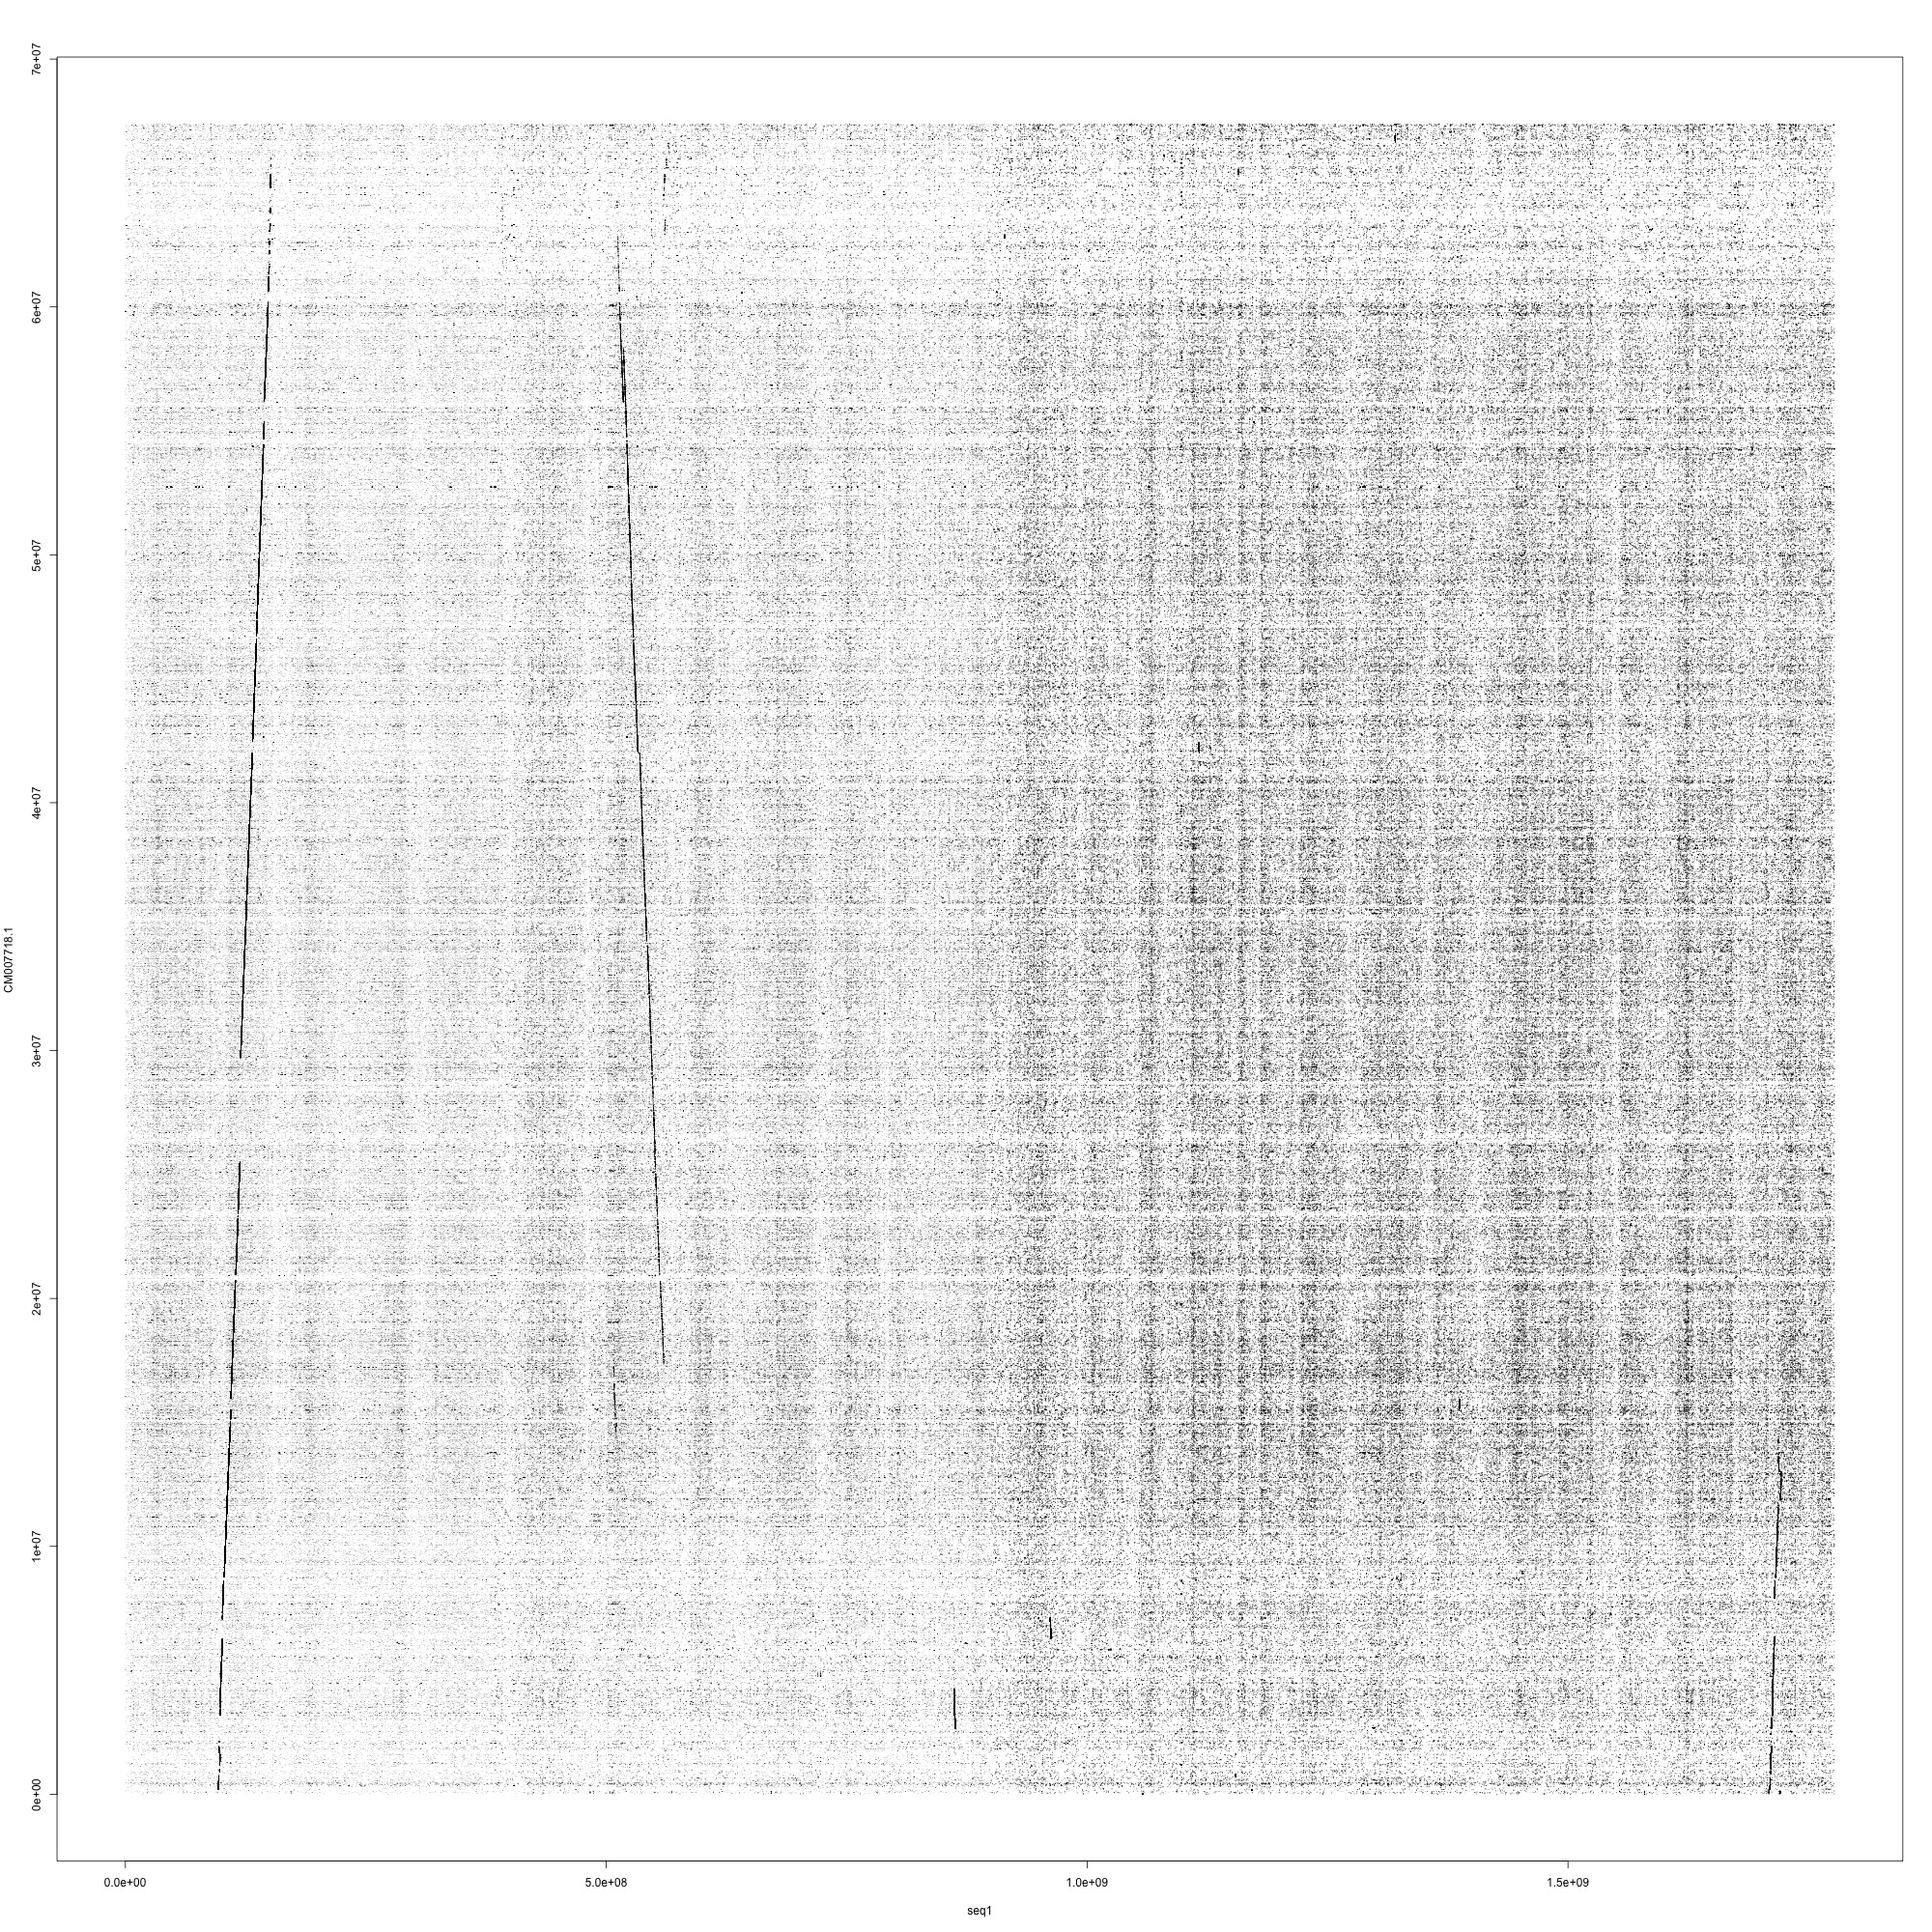
\includegraphics{figs/quickie.jpg}
\caption{Coho Chromo 1 on catenated chinook chromos}
\end{figure}

\hypertarget{explore-the-other-parameters-more}{%
\subsection{Explore the other parameters more}\label{explore-the-other-parameters-more}}

I am going to use the chinook chromosome 1 and coho 10 to explore things that will
clean up the results a little bit.

\begin{Shaded}
\begin{Highlighting}[]
\CommentTok{# in /tmp}
 \VariableTok{i=}\NormalTok{10; }\BuiltInTok{time}\NormalTok{ lastz chinook-1.fna coho-}\VariableTok{$\{i\}}\NormalTok{.fna --notransition --step=20 --nogapped --ambiguous=iupac --format=rdotplot }\OperatorTok{>}\NormalTok{ chinook1_vs_coho}\VariableTok{$\{i\}}\NormalTok{.rdp}\KeywordTok{;}
\ExtensionTok{real}\NormalTok{    0m29.055s}
\ExtensionTok{user}\NormalTok{    0m28.497s}
\ExtensionTok{sys}\NormalTok{ 0m0.413s}
\end{Highlighting}
\end{Shaded}

That is quick enough to explore a few things. Note that we are already doing gap-free extension, because
``By default seeds are extended to HSPs using x-drop extension, with entropy adjustment.'' However, by
default, chaining is not done, and that is the key step in which a path is found through the
high-scoring pairs (HSPs). That doesn't take much (any) extra time and totally cleans things up.

\begin{Shaded}
\begin{Highlighting}[]
\VariableTok{i=}\NormalTok{10; }\BuiltInTok{time}\NormalTok{ lastz chinook-1.fna coho-}\VariableTok{$\{i\}}\NormalTok{.fna --notransition --step=20 --nogapped --ambiguous=iupac --format=rdotplot --chain  }\OperatorTok{>}\NormalTok{ chinook1_vs_coho}\VariableTok{$\{i\}}\NormalTok{.rdp}\KeywordTok{;}

\ExtensionTok{real}\NormalTok{    0m28.704s}
\end{Highlighting}
\end{Shaded}

So, that is greatly improved:

\begin{Shaded}
\begin{Highlighting}[]
\NormalTok{dots <-}\StringTok{ }\NormalTok{readr}\OperatorTok{::}\KeywordTok{read_tsv}\NormalTok{(}\StringTok{"inputs/chain-chinook1_vs_coho10.rdp.gz"}\NormalTok{)}

\KeywordTok{plot}\NormalTok{(dots,}\DataTypeTok{type=}\StringTok{"l"}\NormalTok{)}
\end{Highlighting}
\end{Shaded}

So, it would be worth seeing if chaining also cleans up the multi-chrom alignment:

\begin{Shaded}
\begin{Highlighting}[]
\BuiltInTok{time}\NormalTok{ lastz chinook_nc_chroms.fna[multiple]  coho-1.fna --notransition --step=20 --nogapped --ambiguous=iupac --format=rdotplot --chain }\OperatorTok{>}\NormalTok{ chin_nc_vs_coho1.rdp}

\ExtensionTok{real}\NormalTok{    6m42.835s}
\ExtensionTok{user}\NormalTok{    6m35.042s}
\ExtensionTok{sys}\NormalTok{ 0m6.207s}
\end{Highlighting}
\end{Shaded}

\begin{Shaded}
\begin{Highlighting}[]
\NormalTok{dots <-}\StringTok{ }\NormalTok{readr}\OperatorTok{::}\KeywordTok{read_tsv}\NormalTok{(}\StringTok{"inputs/chin_nc_vs_coho1-chain.rdp.gz"}\NormalTok{)}

\KeywordTok{plot}\NormalTok{(dots,}\DataTypeTok{type=}\StringTok{"l"}\NormalTok{)}
\end{Highlighting}
\end{Shaded}

OK, that shows that it will find crappy chains if given the chance. But if you
zoom in on that stuff you see that some of the spots are pretty short, and some are super
robust. So, we will want some further filtering
to make this work. So, we need to check out the ``back-end filtering.'' that is possible.
Back-end filtering does not happen by default.

Let's say that we want 70 Kb alignment blocks. That is .001 of the total input sequence.

\begin{Shaded}
\begin{Highlighting}[]
\BuiltInTok{time}\NormalTok{ lastz chinook_nc_chroms.fna[multiple]  coho-1.fna --notransition --step=20 --nogapped --ambiguous=iupac --format=rdotplot --chain --coverage=0.1 }\OperatorTok{>}\NormalTok{ chin_nc_vs_coho1-cov-0.1.rdp}
\end{Highlighting}
\end{Shaded}

That took 6.5 minutes again. But, it also produced no output whatsoever. We probably
want to filter on identity first anyway. Because that takes so long, maybe we could
do it with our single chromosome first.

\begin{Shaded}
\begin{Highlighting}[]
\VariableTok{i=}\NormalTok{10; }\BuiltInTok{time}\NormalTok{ lastz chinook-1.fna coho-}\VariableTok{$\{i\}}\NormalTok{.fna --notransition --step=20 --nogapped --ambiguous=iupac --format=rdotplot --chain  }\OperatorTok{>}\NormalTok{ chinook1_vs_coho}\VariableTok{$\{i\}}\NormalTok{.rdp}\KeywordTok{;}
\end{Highlighting}
\end{Shaded}

\begin{Shaded}
\begin{Highlighting}[]
\NormalTok{dots <-}\StringTok{ }\NormalTok{readr}\OperatorTok{::}\KeywordTok{read_tsv}\NormalTok{(}\StringTok{"/tmp/chinook1_vs_coho10-ident95.rdp"}\NormalTok{)}

\KeywordTok{plot}\NormalTok{(dots,}\DataTypeTok{type=}\StringTok{"l"}\NormalTok{)}
\end{Highlighting}
\end{Shaded}

That keeps things very clean, but the alignment blocks are all pretty short (like 50 to 300
bp long). So perhaps we need to do gapped extension here to make these things better. This
turns out to take a good deal longer.

\begin{Shaded}
\begin{Highlighting}[]
\VariableTok{i=}\NormalTok{10; }\BuiltInTok{time}\NormalTok{ lastz chinook-1.fna coho-}\VariableTok{$\{i\}}\NormalTok{.fna --notransition --step=20 --gapped --ambiguous=iupac --format=maf --chain --identity=95  }\OperatorTok{>}\NormalTok{ chinook1_vs_coho}\VariableTok{$\{i\}}\NormalTok{-ident95-gapped.maf}\KeywordTok{;}

\ExtensionTok{real}\NormalTok{    3m15.575s}
\ExtensionTok{user}\NormalTok{    3m14.048s}
\ExtensionTok{sys}\NormalTok{ 0m0.936s}
\end{Highlighting}
\end{Shaded}

\begin{Shaded}
\begin{Highlighting}[]
\NormalTok{dots <-}\StringTok{ }\NormalTok{readr}\OperatorTok{::}\KeywordTok{read_tsv}\NormalTok{(}\StringTok{"/tmp/chinook1_vs_coho10-ident95-gapped.rdp"}\NormalTok{)}
\KeywordTok{plot}\NormalTok{(dots,}\DataTypeTok{type=}\StringTok{"l"}\NormalTok{)}
\end{Highlighting}
\end{Shaded}

That is pretty clean and slick.

Now, this has got me to thinking that maybe I \emph{can} do this on a chromosome by chromosome basis.

Check what 97\% identity looks like:

\begin{Shaded}
\begin{Highlighting}[]
\VariableTok{i=}\NormalTok{10; }\BuiltInTok{time}\NormalTok{ lastz chinook-1.fna coho-}\VariableTok{$\{i\}}\NormalTok{.fna --notransition --step=20 --gapped --ambiguous=iupac --format=rdotplot --chain --identity=97  }\OperatorTok{>}\NormalTok{ chinook1_vs_coho}\VariableTok{$\{i\}}\NormalTok{-ident97-gapped.rdp}\KeywordTok{;}
\end{Highlighting}
\end{Shaded}

\begin{Shaded}
\begin{Highlighting}[]
\NormalTok{dots <-}\StringTok{ }\NormalTok{readr}\OperatorTok{::}\KeywordTok{read_tsv}\NormalTok{(}\StringTok{"/tmp/chinook1_vs_coho10-ident97-gapped.rdp"}\NormalTok{)}
\KeywordTok{plot}\NormalTok{(dots,}\DataTypeTok{type=}\StringTok{"l"}\NormalTok{)}
\end{Highlighting}
\end{Shaded}

That looks to have a few more holes in it.

Final test. Let's see what happens when we chain it on a chromosome that doesn't have
any homology:

\begin{Shaded}
\begin{Highlighting}[]
\CommentTok{# first with no backend filtering}
\VariableTok{i=}\NormalTok{1; }\BuiltInTok{time}\NormalTok{ lastz chinook-1.fna coho-}\VariableTok{$\{i\}}\NormalTok{.fna --notransition --step=20 --gapped --ambiguous=iupac --format=rdotplot --chain  }\OperatorTok{>}\NormalTok{ chinook1_vs_coho}\VariableTok{$\{i\}}\NormalTok{-gapped.rdp}\KeywordTok{;}

\ExtensionTok{real}\NormalTok{    0m35.130s}
\ExtensionTok{user}\NormalTok{    0m34.642s}
\ExtensionTok{sys}\NormalTok{ 0m0.413s}

\CommentTok{# Hey! That is cool.  When there are no HSPs to chain, this doesn't take very long}
\VariableTok{i=}\NormalTok{1; }\BuiltInTok{time}\NormalTok{ lastz chinook-1.fna coho-}\VariableTok{$\{i\}}\NormalTok{.fna --notransition --step=20 --gapped --ambiguous=iupac --format=rdotplot --chain --identity=95 }\OperatorTok{>}\NormalTok{ chinook1_vs_coho}\VariableTok{$\{i\}}\NormalTok{-gapped-ident95.rdp}\KeywordTok{;}
\end{Highlighting}
\end{Shaded}

\begin{Shaded}
\begin{Highlighting}[]
\NormalTok{dots <-}\StringTok{ }\NormalTok{readr}\OperatorTok{::}\KeywordTok{read_tsv}\NormalTok{(}\StringTok{"/tmp/chinook1_vs_coho1-gapped.rdp"}\NormalTok{)}
\KeywordTok{plot}\NormalTok{(dots,}\DataTypeTok{type=}\StringTok{"l"}\NormalTok{)}
\end{Highlighting}
\end{Shaded}

OK, it finds something nice and crappy there.

What about if we require 95\% identity?

\begin{Shaded}
\begin{Highlighting}[]
\NormalTok{dots <-}\StringTok{ }\NormalTok{readr}\OperatorTok{::}\KeywordTok{read_tsv}\NormalTok{(}\StringTok{"/tmp/chinook1_vs_coho1-gapped-ident95.rdp"}\NormalTok{)}
\KeywordTok{plot}\NormalTok{(dots,}\DataTypeTok{type=}\StringTok{"l"}\NormalTok{)}
\end{Highlighting}
\end{Shaded}

That leaves us with very little.

Let's also try interpolation at the end to see how that does. Note that here we also produce the
rdotplot at the same time as the maf.

\begin{Shaded}
\begin{Highlighting}[]
\VariableTok{i=}\NormalTok{10; }\BuiltInTok{time}\NormalTok{ lastz chinook-1.fna coho-}\VariableTok{$\{i\}}\NormalTok{.fna --notransition --step=20 --gapped --ambiguous=iupac --format=maf --rdotplot=chinook1_vs_coho}\VariableTok{$\{i\}}\NormalTok{-ident95-gapped-inner1000.rdp --chain --identity=95 --inner=1000 }\OperatorTok{>}\NormalTok{ chinook1_vs_coho}\VariableTok{$\{i\}}\NormalTok{-ident95-gapped-inner1000.maf}\KeywordTok{;}

\ExtensionTok{real}\NormalTok{    4m25.625s}
\ExtensionTok{user}\NormalTok{    4m22.957s}
\ExtensionTok{sys}\NormalTok{ 0m1.478s}
\end{Highlighting}
\end{Shaded}

That took an extra minute, but was not so bad.

\begin{Shaded}
\begin{Highlighting}[]
\NormalTok{dots <-}\StringTok{ }\NormalTok{readr}\OperatorTok{::}\KeywordTok{read_tsv}\NormalTok{(}\StringTok{"/tmp/chinook1_vs_coho10-ident95-gapped-inner1000.rdp"}\NormalTok{)}
\KeywordTok{plot}\NormalTok{(dots,}\DataTypeTok{type=}\StringTok{"l"}\NormalTok{)}
\end{Highlighting}
\end{Shaded}

\hypertarget{repeat-masking-the-coho-genome}{%
\subsubsection{Repeat Masking the Coho genome}\label{repeat-masking-the-coho-genome}}

Turns out that NCBI site has the repeat masker output in GCF\_002021735.1\_Okis\_V1\_rm.out.gz.
I save that to a shorter name. Now I will make a bed file of the repeat regions. Then I use bedtools maskfasta to softmask that fasta file.

\begin{Shaded}
\begin{Highlighting}[]
\CommentTok{# in: /Users/eriq/Documents/UnsyncedData/Okis_v1}
\ExtensionTok{gzcat}\NormalTok{ Okis_V1_rm.out.gz }\KeywordTok{|} \FunctionTok{awk} \StringTok{'NR>3 \{printf("%s\textbackslash{}t%s\textbackslash{}t%s\textbackslash{}n", $5, $6, $7)\}'} \OperatorTok{>}\NormalTok{ repeat-regions.bed }

\ExtensionTok{bedtools}\NormalTok{ maskfasta -fi Okis_V1.fna -bed repeat-regions.bed  -fo Okis_V1-soft-masked.fna  -soft}
\end{Highlighting}
\end{Shaded}

That works great. But it turns out that the coho genome is already softmasked.

But, it is good to now that I can use a repeat mask output file to toss repeat
sites if I want to for ANGSD analyses, etc.

\hypertarget{multiz-maf2fasta}{%
\subsubsection{multiz maf2fasta}\label{multiz-maf2fasta}}

So, it looks like you can use single\_cov2 from multiz to retain only a single
alignment block covering each area. Then you can maf2fasta that and send it off in
fasta format. Line2 holds the reference (target) sequence, but it has dashes added where
the query has stuff not appearing in the target. So, what you have to do is run through that sequence and drop all the positions in the query that correspond to dashes in the
target. That will get us what we want.

But maybe I can just use megablast like Christensen and company. They have some of their
scripts, but it is not clear to me that it will be easy to get that back to a fasta
for later analysis in ANGSD.

Not only that, but then there is the whole paralog issue. I am exploring that a little
bit right now. It looks like when you crank the identity requirement up, the paralogs
get pretty spotty so they can be easily recognized. For example setting the identity
at 99.5 makes it clear which is the paralog:

\begin{Shaded}
\begin{Highlighting}[]
\BuiltInTok{time}\NormalTok{ lastz chinook_nc_chroms.fna[multiple]  coho-1.fna --notransition --step=20 --nogapped --ambiguous=iupac --format=rdotplot --chain --identity=99.5 }\OperatorTok{>}\NormalTok{ chin_nc_vs_coho1-chain-ident-99.5.rdp}
\CommentTok{# takes about 6 minutes}
\end{Highlighting}
\end{Shaded}

And the figure is here.

\begin{figure}
\centering
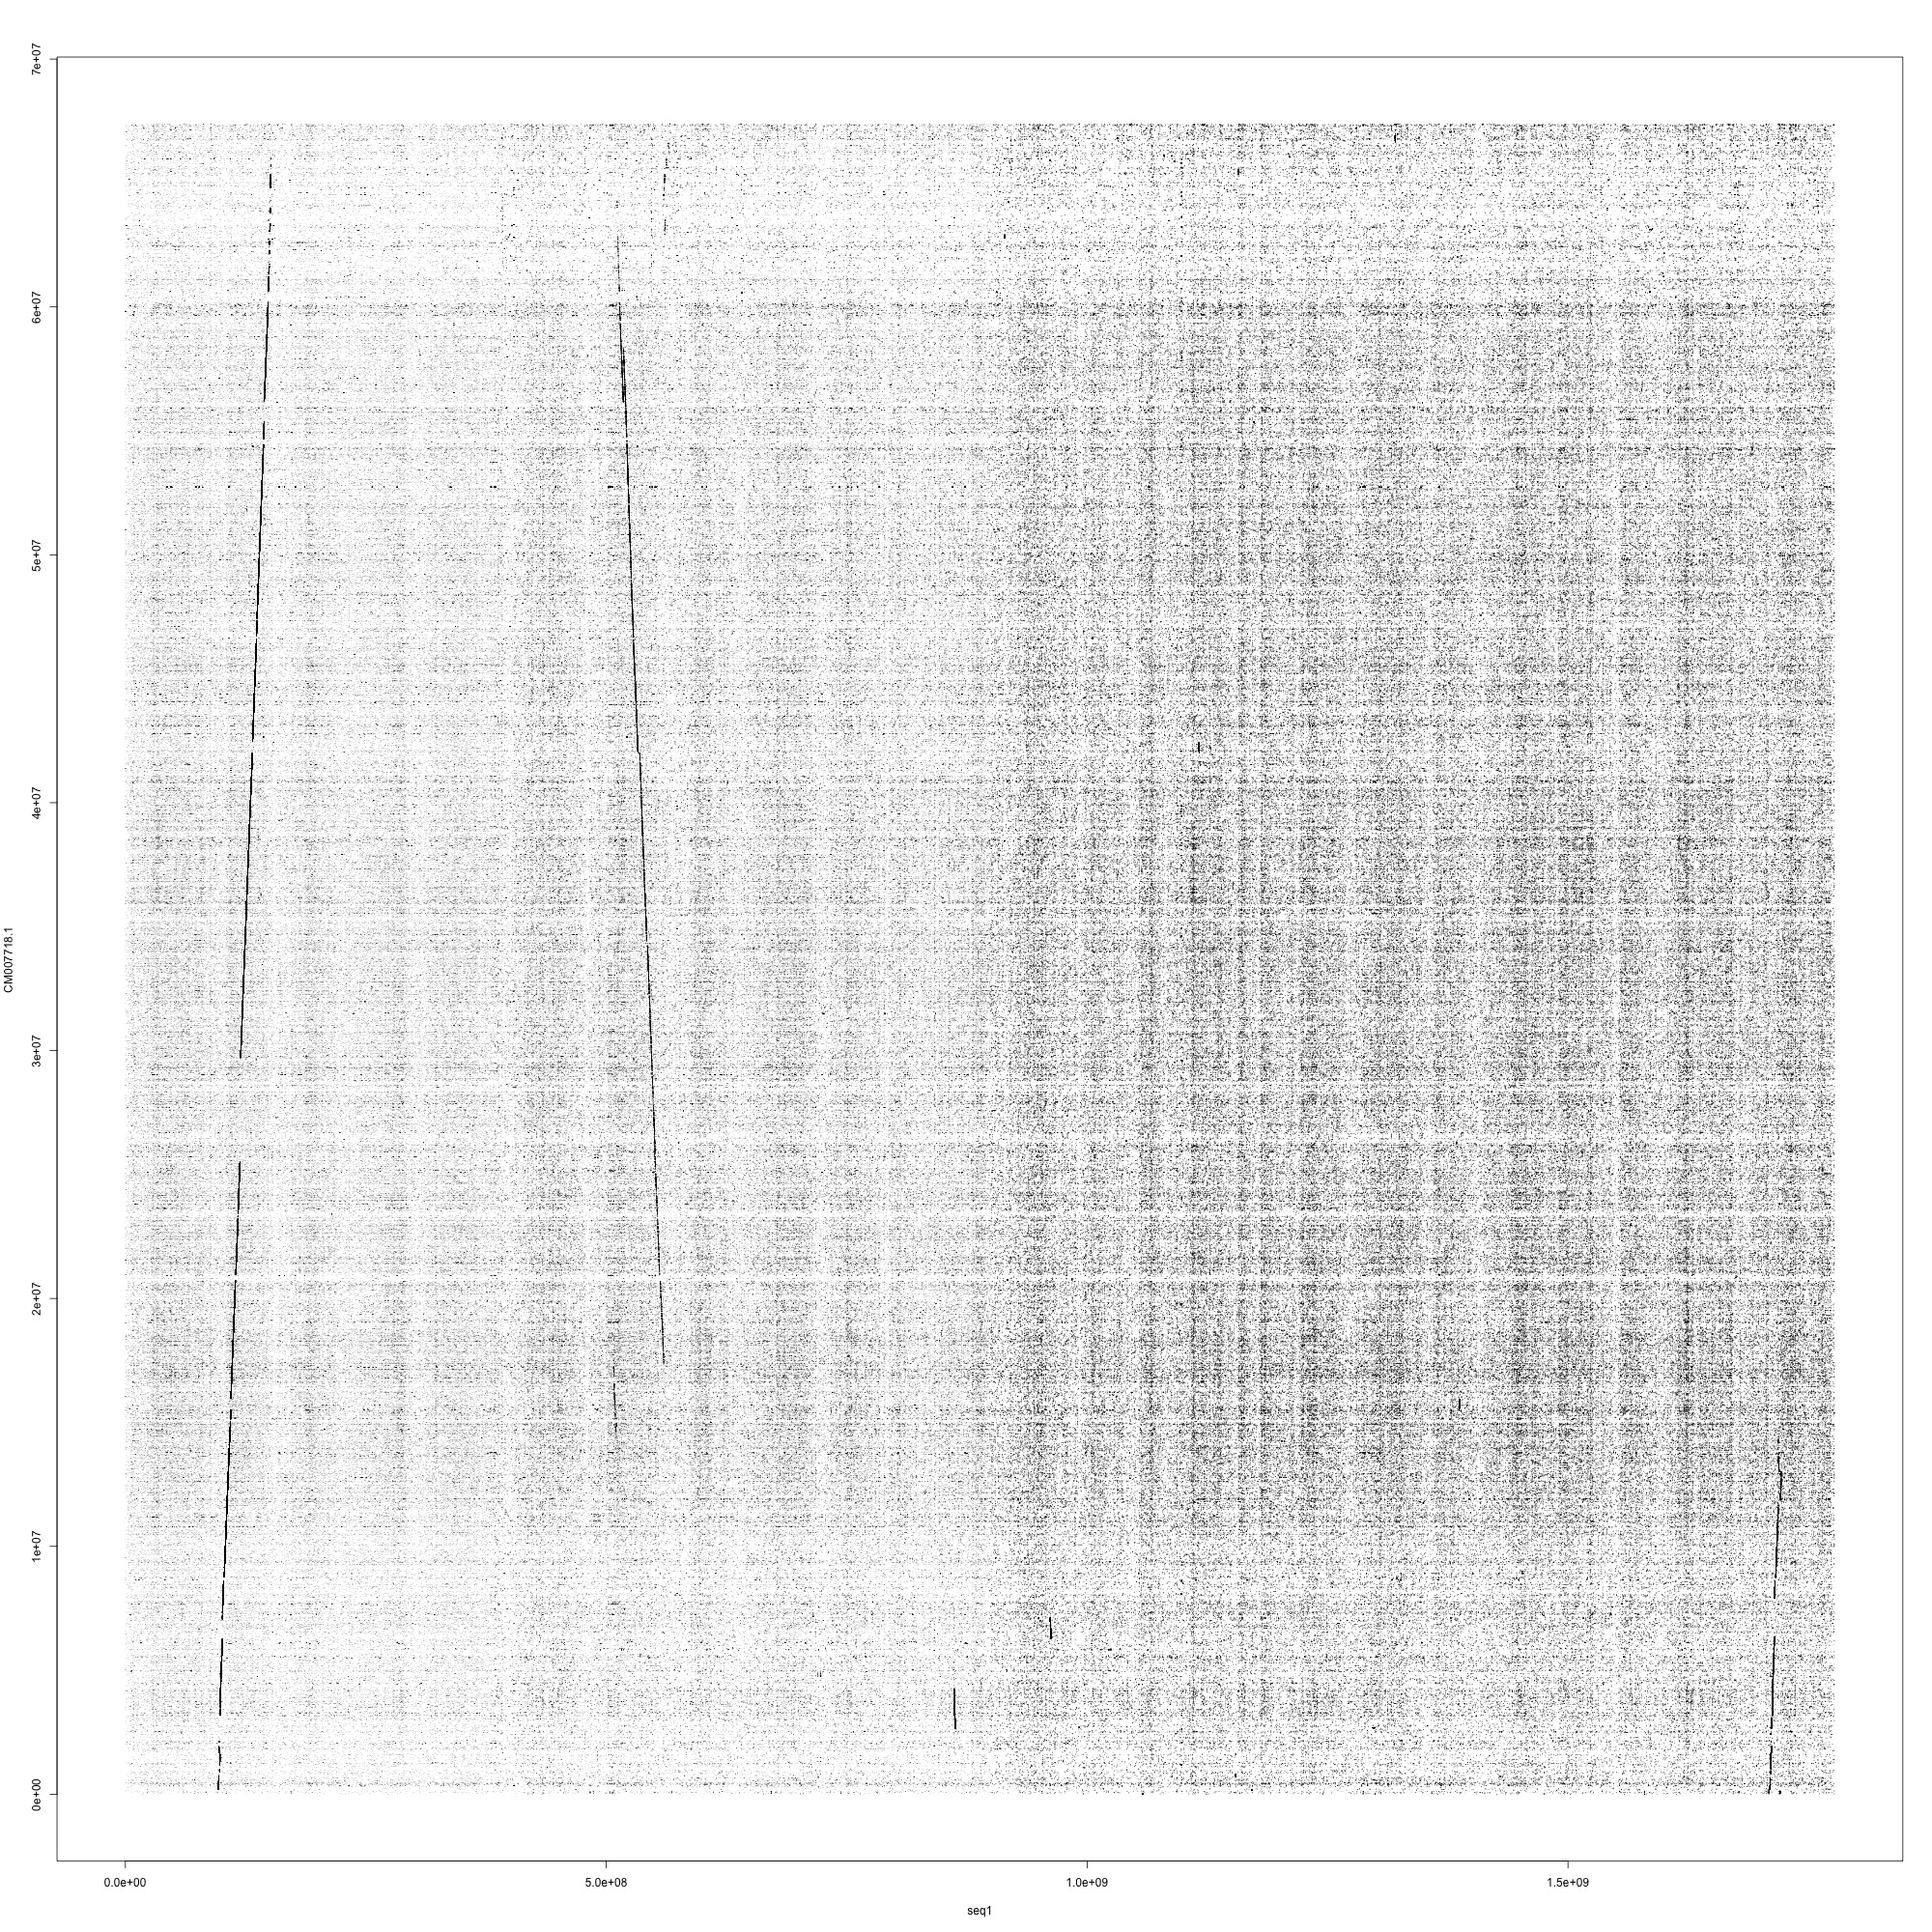
\includegraphics{figs/quickie.jpg}
\caption{Coho Chromo 1 on catenated chinook chromos. Ident=99.5}
\end{figure}

So, I think this is going to be a decent workflow:

\begin{enumerate}
\def\labelenumi{\arabic{enumi}.}
\tightlist
\item
  run lastz on each coho linkage group against each chinook chromosome separately. Do this at identity=92 and identity=95 and identity=99.9. For each run, produce a .maf file and
  at the same time a .rdotplot output.
\item
  Combine all the .rdotplot files together into something that can be faceted over
  chromosomes and make a massive facet grid showing the results for all chromosomes.
  Do this at different identity levels so that the paralogs can be distinguished.
\item
  Visually look up each columns of those plots and determine which coho chromosomes
  carry homologous material for each chinook chromosome. For each such chromosome pair,
  run single\_cov2 on them (maybe on the ident=92 version).
\item
  Then merge those MAFs. Probably can just cat them together, but there might be some
  sorting that needs to be done on them.
\item
  Run maf2fasta on those merged mafs to get a fasta for each chinook chromosome.
\item
  Write a C-program that uses uthash to efficiently read the fasta for each chinook
  chromosome and then write out a version in which the positions that are dashes in the
  chinook reference are removed from both the chinook reference and the aligned coho
  sequence. \_Actually, one can just pump each sequence out to a separate file in which
  each site occupies one line. Then paste those and do the comparison\ldots{}
\end{enumerate}

\begin{Shaded}
\begin{Highlighting}[]
\ExtensionTok{2018-10-18}\NormalTok{ 11:15 /tmp/--% time (awk }\StringTok{'NR==2'}\NormalTok{ splud }\KeywordTok{|} \ExtensionTok{fold}\NormalTok{ -w1 }\OperatorTok{>}\NormalTok{ spp1.text)}

\ExtensionTok{real}\NormalTok{    0m23.244s}
\ExtensionTok{user}\NormalTok{    0m22.537s}
\ExtensionTok{sys}\NormalTok{ 0m0.685s}

\CommentTok{# then you can use awk easily like this:}
\ExtensionTok{paste}\NormalTok{ spp1.text spp2.text }\KeywordTok{|} \FunctionTok{awk} \StringTok{'BEGIN \{SUBSEP = " "\} \{n[$1,$2]++\} END \{for(i in n) print i, n[i]\}'} 
\end{Highlighting}
\end{Shaded}

\begin{enumerate}
\def\labelenumi{\arabic{enumi}.}
\setcounter{enumi}{6}
\tightlist
\item
  The coho sequence thus obtained will have dashes anywhere there isn't coho aligned
  to the chinook. So, first, for each chromosome I can count the number of dashes, which
  will tell me the fraction of sites on the chinook genome that were aligned (sort of---there is an issue with N's in the coho genome.) Then those dashes can be converted to N's.
\item
  It would be good to count the number of sites that are not N's in chinook that are also
  not Ns in coho, to know how much of it we have aligned.
\end{enumerate}

Note, the last thing that really remains here is making sure that I can run two or more different query sequences against one chinook genome and then process that out correctly
into a fasta.

Note that Figure 1 in christensen actually gives me a lot to go on in terms of which
chromosomes in coho to map against which ones in chinook.

\hypertarget{part-part-iv-analysis-of-big-variant-data}{%
\part{Part IV: Analysis of Big Variant Data}\label{part-part-iv-analysis-of-big-variant-data}}

\hypertarget{bioinformatic-analysis-on-variant-data}{%
\chapter{Bioinformatic analysis on variant data}\label{bioinformatic-analysis-on-variant-data}}

Standard analyses like computing Fst and linkage disequilibrium, etc., from
data, typically in a VCF file.

Basically, we want to get comfortable with plink 2.0, bedtools, vcftools, etc.

The key in all of this is to motivate every single thing we do here in terms of an
application in conservation genomics. That is going to be key.

This Part IV will be about standard bioinformatic tools for doing things
with big variant data.

\begin{itemize}
\tightlist
\item
  Filtering
\item
  Imputation
\item
  LD, HWD, FST
\item
  Etc.
\end{itemize}

I will probably have a chapter on unix tools.

Maybe another on R/Bioconductor tools.

Gotta have a chapter about ``Look at your data!'' and Whoa! and diagnostics
using radiator.

\hypertarget{part-part-v-population-genomics}{%
\part{Part V: Population Genomics}\label{part-part-v-population-genomics}}

\hypertarget{topics-in-pop-gen}{%
\chapter{Topics in pop gen}\label{topics-in-pop-gen}}

This is just a bunch of ideas. But basically, I want to have some topics here that
everyone should know about. Slanted toward things that are relevant for inference
or simulation.

\hypertarget{coalescent}{%
\section{Coalescent}\label{coalescent}}

Gotta have a lecture on the coalescent. It would be nice to try to motivate
all the topics from this backward in time perspective.

Get far enough to discuss \(\pi\) and the expected site frequency spectrum.

\hypertarget{measures-of-genetic-diversity-and-such}{%
\section{Measures of genetic diversity and such}\label{measures-of-genetic-diversity-and-such}}

It would really be good for me to write a chapter / give a few lectures
on different measures like dxy and fst

From Ash's paper: However, population genomic analyses (outlined below) use FST only, as dxy was highly correlated to nucleotide diversity (for early stage diverging populations the correlation between dxy and \(\pi\) is \textgreater{} 0.91, Pearson correlation). As such variation in dxy across the genome reflects variation in diversity, not differentiation (Riesch et al., 2017).

Tajima's \(D\) and such. The influence of selection on such measures.

\hypertarget{demographic-inference-with-partial-a-partial-i-and-moments}{%
\section{\texorpdfstring{Demographic inference with \(\partial a \partial i\) and \emph{moments}}{Demographic inference with \textbackslash{}partial a \textbackslash{}partial i and moments}}\label{demographic-inference-with-partial-a-partial-i-and-moments}}

\hypertarget{balls-in-boxes}{%
\section{Balls in Boxes}\label{balls-in-boxes}}

Would be worthwhile to have a review of all these sorts of variants of
population assignment, structure, admixture, etc.

Population structure and PCAs.

finestructure and fineRADstructure.

Might want to insert \citet{BradburdInferringContinuousDiscrete2018}.

Might also want to discuss \citet{PickrellInferencePopulationSplits2012}.

Also: \citet{PritchardInferencePopulationStructure2000}

What if we go and try to put the same one in? Like Pritch 2000 again: \citep{PritchardInferencePopulationStructure2000}

\hypertarget{some-landscape-genetics}{%
\section{Some landscape genetics}\label{some-landscape-genetics}}

After talking with Amanda about her dissertation I realized it would be good
to talk about some landscape genetics stuff. For sure I want to talk about
EEMS and maybe CircuitScape, just so I know well what is going on with the
latter.

\hypertarget{relationship-inference}{%
\section{Relationship Inference}\label{relationship-inference}}

Maybe do a lecture on this\ldots{}

\hypertarget{tests-for-selection}{%
\section{Tests for Selection}\label{tests-for-selection}}

A look at a selection of the methods that are out there. FST outliers, \emph{Bayescan}, \emph{Lositan}, \emph{PCAdapt}, and friends. It would be good to get a nice succinct explanation/understanding of all of these.

\hypertarget{multivariate-associations-gea-etc.}{%
\section{Multivariate Associations, GEA, etc.}\label{multivariate-associations-gea-etc.}}

It really is time for me to wrap my head around this stuff.

\hypertarget{estimating-heritability-in-the-wild}{%
\section{Estimating heritability in the wild}\label{estimating-heritability-in-the-wild}}

Another from Amanda. It would be good to do some light Quant Genet so that
we all understand how we might be able to use NGS data to estimate heritability
in wild populations.

\bibliography{references.bib,book.bib}

\backmatter
\printindex

\end{document}
